% This is the Reed College LaTeX thesis template. Most of the work
% for the document class was done by Sam Noble (SN), as well as this
% template. Later comments etc. by Ben Salzberg (BTS). Additional
% restructuring and APA support by Jess Youngberg (JY).
% Your comments and suggestions are more than welcome; please email
% them to cus@reed.edu
%
% See https://www.reed.edu/cis/help/LaTeX/index.html for help. There are a
% great bunch of help pages there, with notes on
% getting started, bibtex, etc. Go there and read it if you're not
% already familiar with LaTeX.
%
% Any line that starts with a percent symbol is a comment.
% They won't show up in the document, and are useful for notes
% to yourself and explaining commands.
% Commenting also removes a line from the document;
% very handy for troubleshooting problems. -BTS

% As far as I know, this follows the requirements laid out in
% the 2002-2003 Senior Handbook. Ask a librarian to check the
% document before binding. -SN

%%
%% Preamble
%%
% \documentclass{<something>} must begin each LaTeX document
\documentclass[12pt,oneside]{reedthesis}
% Packages are extensions to the basic LaTeX functions. Whatever you
% want to typeset, there is probably a package out there for it.
% Chemistry (chemtex), screenplays, you name it.
% Check out CTAN to see: https://www.ctan.org/
%%
\usepackage{graphicx,latexsym}
\usepackage{amsmath}
\usepackage{amssymb,amsthm}
\usepackage{longtable,booktabs,setspace}
\usepackage{chemarr} %% Useful for one reaction arrow, useless if you're not a chem major
\usepackage[hyphens]{url}
% Added by CII
\usepackage{hyperref}
\usepackage{lmodern}
\usepackage{float}
\floatplacement{figure}{H}
% Thanks, @Xyv
\usepackage{calc}
% End of CII addition
\usepackage{rotating}

% Next line commented out by CII
%%% \usepackage{natbib}
% Comment out the natbib line above and uncomment the following two lines to use the new
% biblatex-chicago style, for Chicago A. Also make some changes at the end where the
% bibliography is included.
%\usepackage{biblatex-chicago}
%\bibliography{thesis}
% \ifxetex
%   \usepackage{polyglossia}
%   \setmainlanguage{spanish}
%   % Tabla en lugar de cuadro
%   \gappto\captionsspanish{\renewcommand{\tablename}{Tabla}
%           \renewcommand{\listtablename}{Índice de tablas}}
% \else
%   \usepackage[spanish,es-tabla]{babel}
% \fi

% Added by CII (Thanks, Hadley!)
% Use ref for internal links
\renewcommand{\hyperref}[2][???]{\autoref{#1}}
\def\chapterautorefname{chapter}
\def\sectionautorefname{section}
\def\subsectionautorefname{subsection}
% End of CII addition

% Added by CII
\usepackage{caption}
\captionsetup{width=5in}
% End of CII addition

% \usepackage{times} % other fonts are available like times, bookman, charter, palatino

% Syntax highlighting #22

% To pass between YAML and LaTeX the dollar signs are added by CII
\title{Utilización de datos satelitales para la evaluación y mejora de los pronósticos numéricos en alta resolución a muy corto plazo}
\author{Lic. Paola Corrales}
% The month and year that you submit your FINAL draft TO THE LIBRARY (May or December)
\date{BUENOS AIRES, 2023}
\division{Facultad de Ciencias Exactas y Naturales}
\advisor{Vito Galligani}
\institution{Universidad de Buenos Aires}
\degree{Tesis presentada para optar al título de Doctora de la Universidad de Buenos Aires en el Área de Ciencias de la Atmósfera y los Océanos}
%If you have two advisors for some reason, you can use the following
% Uncommented out by CII
\altadvisor{Juan Ruiz}
\consejera{Celeste Saulo}
\place{Centro de Investigaciones del Mar y la Atmósfera. CONICET-UBA}
% End of CII addition

%%% Remember to use the correct department!
\department{Departamento de Ciencias de la Atmósfera y los Océanos}
% if you're writing a thesis in an interdisciplinary major,
% uncomment the line below and change the text as appropriate.
% check the Senior Handbook if unsure.
%\thedivisionof{The Established Interdisciplinary Committee for}
% if you want the approval page to say "Approved for the Committee",
% uncomment the next line
%\approvedforthe{Committee}

% Added by CII
%%% Copied from knitr
%% maxwidth is the original width if it's less than linewidth
%% otherwise use linewidth (to make sure the graphics do not exceed the margin)
\makeatletter
\def\maxwidth{ %
  \ifdim\Gin@nat@width>\linewidth
    \linewidth
  \else
    \Gin@nat@width
  \fi
}
\makeatother

\makeatletter
\renewcommand{\@chapapp}{Capítulo}
\makeatother

% From {rticles}

\renewcommand{\contentsname}{Índice}
% End of CII addition

\setlength{\parskip}{0pt}

% Added by CII

\providecommand{\tightlist}{%
  \setlength{\itemsep}{0pt}\setlength{\parskip}{0pt}}

\Acknowledgements{
I want to thank a few people.
}

\Dedication{

}

\Preface{

}

\Abstract{
\hypertarget{use-of-satellite-data-for-the-evaluation-and-improvement-of-short-term-high-resolution-numerical-forecasts}{%
\section*{Use of satellite data for the evaluation and improvement of short-term high-resolution numerical forecasts}\label{use-of-satellite-data-for-the-evaluation-and-improvement-of-short-term-high-resolution-numerical-forecasts}}
\addcontentsline{toc}{section}{Use of satellite data for the evaluation and improvement of short-term high-resolution numerical forecasts}

In Argentina, extreme weather events cause considerable human and material losses. Many of these phenomena, such as tornadoes, intense gusts, extreme rainfall in short periods, large hail, and electrical activity, are associated with deep convection. It is, therefore, necessary to advance in the knowledge of these phenomena and in the ability to forecast their occurrence. The forecasting of severe phenomena is a very complex scientific and technological challenge due to the limited predictability at the mesoscale and the difficulty of knowing or diagnosing the state of the atmosphere at small spatial scales and short times (for example, from 1 to 10 km and in the order of minutes). Data assimilation (DA) at the mesoscale is an approach that can provide suitable initial conditions for generating high-resolution numerical forecasts and is therefore an evolving area of study.

For data assimilation methods to be successful, observational networks with a sufficient temporal and spatial resolution capable of capturing mesoscale variability must be used. The relative scarcity of conventional observations in South America poses an important challenge that can be solved with the use of other sources of observations such as automatic surface stations, winds derived from satellite observations, and radiances from polar and geostationary satellites in clear sky. In this context, this thesis work sought to quantify and compare the impact of each of the data sets in a mesoscale assimilation system.

The study of radiance assimilation at the regional level is even more important in South America since no previous studies have been carried out. For this reason, special emphasis is placed on direct radiance assimilation and the quality controls necessary to work with these observations. First, the impact of the assimilation of polar satellite observations with sensors sensitive to the infrared and microwave spectrum is studied. Secondly, we study the implementation of the assimilation of observations from the GOES-16 geostationary satellite and the impact of assimilating observations at high spatial and temporal resolution in a regional context.

To achieve the objectives of this thesis, different data assimilation experiments were performed for a case study of an MCS that developed over southern South America during November 22-23, 2018 during the intense observing period of the RELAMPAGO field campaign. The WRF-GSI-LETFK system was used for the generation of frequently update ensemble-based experiments. While the WRF model is one of the most used and in constant advance, with important antecedents in Argentina, the GSI assimilation system, and in particular its LETKF version, has not been tested in Argentina and is one of the original contributions of this thesis.

The results obtained show that the assimilation of observations with high temporal and spatial frequency generates an important impact on the planetary boundary layer correcting the warm and dry bias present in the model and generating a better development of deep convection and precipitation for the case study. The assimilation of the radiance observations produced a better development of convection leading to an increase in accumulated precipitation. The ensemble forecast initialized from each experiment also showed improvements in the precipitation representation. Finally, the implementation of GOES-16 observation assimilation was shown to be good producing precipitation forecasts closer to the observed. In particular, the sensitivity experiments generated to analyze the impact of assimilating observations from the three water vapor channels showed that channel 10, associated with water vapor content at low levels, is the one that provides the most information, particularly when the observations are assimilated using a spatial resolution similar to that of the model (10 km).

\textbf{Key words:} Data assimilation, Mesoescale, Convencional observations, Satellite observations, Forecasts
}

	\usepackage{setspace}\onehalfspacing
\usepackage[spanish,es-tabla]{babel}
	\usepackage{booktabs}
\usepackage{longtable}
\usepackage{array}
\usepackage{multirow}
\usepackage{wrapfig}
\usepackage{float}
\usepackage{colortbl}
\usepackage{pdflscape}
\usepackage{tabu}
\usepackage{threeparttable}
\usepackage{threeparttablex}
\usepackage[normalem]{ulem}
\usepackage{makecell}
\usepackage{xcolor}
% End of CII addition
%%
%% End Preamble
%%
%
\begin{document}

% Everything below added by CII
  \maketitle

\frontmatter % this stuff will be roman-numbered
\pagestyle{empty} % this removes page numbers from the frontmatter
  \begin{resumen}
    \hypertarget{utilizaciuxf3n-de-datos-satelitales-para-la-evaluaciuxf3n-y-mejora-de-los-pronuxf3sticos-numuxe9ricos-en-alta-resoluciuxf3n-a-muy-corto-plazo}{%
    \section*{Utilización de datos satelitales para la evaluación y mejora de los pronósticos numéricos en alta resolución a muy corto plazo}\label{utilizaciuxf3n-de-datos-satelitales-para-la-evaluaciuxf3n-y-mejora-de-los-pronuxf3sticos-numuxe9ricos-en-alta-resoluciuxf3n-a-muy-corto-plazo}}
    \addcontentsline{toc}{section}{Utilización de datos satelitales para la evaluación y mejora de los pronósticos numéricos en alta resolución a muy corto plazo}
    
    En la Argentina, los fenómenos meteorológicos extremos producen cuantiosas pérdidas humanas y materiales. Muchos de estos fenómenos, por ejemplo tornados, ráfagas intensas, precipitaciones extremas en cortos períodos de tiempo, granizo de gran tamaño y actividad eléctrica, están asociados a la ocurrencia de convección profunda. Es por tal motivo necesario avanzar en el conocimiento de estos fenómenos y en la capacidad de pronosticar la ocurrencia de los mismos. El pronóstico de los fenómenos severos es un desafío científico y tecnológico muy complejo debido a la predictibilidad limitada en la mesoescala y a la dificultad de conocer o diagnosticar el estado de la atmósfera en escalas espaciales pequeñas y tiempos cortos (por ejemplo de 1 a 10 km y del orden de los minutos). La asimilación de datos (AD) en la mesoescala es un enfoque que puede proporcionar condiciones iniciales adecuadas para generar pronósticos numéricos de alta resolución y, por tanto, es un área de estudio en constante evolución.
    
    Para que los métodos de asimilación de datos tengan éxito, deben utilizarse redes de observación con suficiente resolución temporal y espacial capaces de captar la variabilidad de la mesoescala. La relativa escasez de observaciones convencionales en Sudamérica supone un importante desafío que puede ser resuelto con el uso de otras fuentes de observaciones como estaciones de superficie automáticas, vientos derivados de observaciones satelitales y radiancias de satélites polares y geoestacionarios en cielo claro. En este contexto, este trabajo de tésis buscó cuantificar y comparar el impacto de cada uno de los conjuntos de datos en un sistema de asimilación de mesoescala.
    
    El estudio de la asimilación de radiancias a nivel regional cobra aún mayor importancia en Sudamérica ya que no se conocen estudios realizados previamente. Por esta razón, en este trabajo se hace especial énfasis en la asimilación directa de radiancias y los controles de calidad necesarios para trabajar con estas observaciones. En primer lugar se estudia el impacto de la asimilación de observaciones de satélites polares con sensores sensibles al espectro infrarrojo y microondas. Y en segundo lugar, se estudia la implementación de la asimilación de observaciones del satélite geoestacionario GOES-16 y el impacto de asimilar observaciones en alta resolución espacial y temporal en un contexto regional.
    
    Para alcanzar los objetivos de esta tésis, se realizaron distintos experimentos de asimilación de datos aplicados a un estudio de caso de un SCM que se desarrolló sobre el sur de Sudamérica durante el 22 y 23 de noviembre de 2018 durante el período de observación intensa de la campaña de campo RELAMPAGO. Se utilizó el sistema WRF-GSI-LETFK para la generación de los experimentos de actualización frecuente y basados en ensambles. Mientras que el modelo WRF es uno de los más utilizados y en constante avance, con importantes antecedentes en Argentina, el sistema de asimilación GSI y en particular su versión de LETKF, no ha sido probado en Argentina y es uno de los aportes originales de esta tesis.
    
    Los resultados obtenidos muestran que la asimilación de observaciones con alta frecuencia temporal y espacial genera un importante impacto en la capa límite planetaria corrigiendo el bias cálido y seco presente en el modelo generando un mejor desarrollo de la convección profunda y la precipitación para el caso de estudio. La asimilación de las observaciones de radiancia produjo un mejor desarrollo de la convección conduciendo a un aumento de la precipitación acumulada. El pronóstico por ensambles inicializado a partir de cada experimento también mostró mejoras en la representación de la precipitación. Finalmente la implementación de la asimilación de observaciones de GOES-16 mostró ser adecuada produciendo pronósticos de precipitación más cercanos a lo observado. En particular los experimentos de sensibilidad generados para analisis el impacto de asimilar observaciones de los tres canales de vapor de agua mostraron que el canal 10, asociado al contenido de vapor de agua en niveles bajos, es el que aporta mayor información, particularmente cuando las observaciones son asimiladas utilizando una resolución espacial similar a la del modelo (10 km).
    
    \textbf{Palabras claves:} Asimilación de datos, Mesoescala, Observaciones convencionales, Observaciones de satélite, Pronósticos
  \end{resumen}
  \begin{abstract}
    \hypertarget{use-of-satellite-data-for-the-evaluation-and-improvement-of-short-term-high-resolution-numerical-forecasts}{%
    \section*{Use of satellite data for the evaluation and improvement of short-term high-resolution numerical forecasts}\label{use-of-satellite-data-for-the-evaluation-and-improvement-of-short-term-high-resolution-numerical-forecasts}}
    \addcontentsline{toc}{section}{Use of satellite data for the evaluation and improvement of short-term high-resolution numerical forecasts}
    
    In Argentina, extreme weather events cause considerable human and material losses. Many of these phenomena, such as tornadoes, intense gusts, extreme rainfall in short periods, large hail, and electrical activity, are associated with deep convection. It is, therefore, necessary to advance in the knowledge of these phenomena and in the ability to forecast their occurrence. The forecasting of severe phenomena is a very complex scientific and technological challenge due to the limited predictability at the mesoscale and the difficulty of knowing or diagnosing the state of the atmosphere at small spatial scales and short times (for example, from 1 to 10 km and in the order of minutes). Data assimilation (DA) at the mesoscale is an approach that can provide suitable initial conditions for generating high-resolution numerical forecasts and is therefore an evolving area of study.
    
    For data assimilation methods to be successful, observational networks with a sufficient temporal and spatial resolution capable of capturing mesoscale variability must be used. The relative scarcity of conventional observations in South America poses an important challenge that can be solved with the use of other sources of observations such as automatic surface stations, winds derived from satellite observations, and radiances from polar and geostationary satellites in clear sky. In this context, this thesis work sought to quantify and compare the impact of each of the data sets in a mesoscale assimilation system.
    
    The study of radiance assimilation at the regional level is even more important in South America since no previous studies have been carried out. For this reason, special emphasis is placed on direct radiance assimilation and the quality controls necessary to work with these observations. First, the impact of the assimilation of polar satellite observations with sensors sensitive to the infrared and microwave spectrum is studied. Secondly, we study the implementation of the assimilation of observations from the GOES-16 geostationary satellite and the impact of assimilating observations at high spatial and temporal resolution in a regional context.
    
    To achieve the objectives of this thesis, different data assimilation experiments were performed for a case study of an MCS that developed over southern South America during November 22-23, 2018 during the intense observing period of the RELAMPAGO field campaign. The WRF-GSI-LETFK system was used for the generation of frequently update ensemble-based experiments. While the WRF model is one of the most used and in constant advance, with important antecedents in Argentina, the GSI assimilation system, and in particular its LETKF version, has not been tested in Argentina and is one of the original contributions of this thesis.
    
    The results obtained show that the assimilation of observations with high temporal and spatial frequency generates an important impact on the planetary boundary layer correcting the warm and dry bias present in the model and generating a better development of deep convection and precipitation for the case study. The assimilation of the radiance observations produced a better development of convection leading to an increase in accumulated precipitation. The ensemble forecast initialized from each experiment also showed improvements in the precipitation representation. Finally, the implementation of GOES-16 observation assimilation was shown to be good producing precipitation forecasts closer to the observed. In particular, the sensitivity experiments generated to analyze the impact of assimilating observations from the three water vapor channels showed that channel 10, associated with water vapor content at low levels, is the one that provides the most information, particularly when the observations are assimilated using a spatial resolution similar to that of the model (10 km).
    
    \textbf{Key words:} Data assimilation, Mesoescale, Convencional observations, Satellite observations, Forecasts
  \end{abstract}

  \begin{acknowledgements}
    I want to thank a few people.
  \end{acknowledgements}
  \hypersetup{linkcolor=black}
  \setcounter{secnumdepth}{2}
  \setcounter{tocdepth}{2}
  \tableofcontents

  \listoftables

  \listoffigures

\mainmatter % here the regular arabic numbering starts
\pagestyle{fancyplain} % turns page numbering back on

\hypertarget{introducciuxf3n}{%
\chapter{Introducción}\label{introducciuxf3n}}

\hypertarget{pronostico-de-eventos-severos}{%
\section{Pronostico de eventos severos}\label{pronostico-de-eventos-severos}}

La predicción de fenómenos meteorológicos extremos es de particular importancia ya que pueden producir cuantiosas pérdidas humanas y materiales. En Argentina, una gran cantidad de estos fenómenos están asociados a la ocurrencia de convección profunda entre los que se cuentan tornados, ráfagas intensas, precipitaciones extremas en cortos períodos de tiempo, granizo de gran tamaño y actividad eléctrica. Es por tal motivo necesario avanzar en el conocimiento de estos procesos y la dinamica de la convección y en la capacidad de pronosticar la ocurrencia de los mismos.

La simulación numérica de la atmósfera, es decir, la integración de las ecuaciones que rigen la evolución del sistema atmósferico es la base para el pronostico numerico del tiempo en diversas escalas temporales desde horas a semanas.

El pronostico meteorologico es un problema de condiciones iniciales y de borde. Si se cuenta con condiciones de borde apropiadas, es decir, una correcta representación de las características de la superficie terrestre y el tope de la atmósfera, la generación de pronósticos de calidad dependerá entonces, de la capacidad del modelo para representar los procesos atmosféricos y y el conocimiento del estado inicial de la atmosfera (Kalnay, 2002).

El pronóstico de fenomenos extremos asociados a conveccion profunda es a su vez un desafío científico y tecnológico muy complejo debido a la predictibilidad limitada en la mesoescala. En particular, en la mesoescala la conveccion humeda esta dentro de los fenemos mas impredecibles debido a que se asocia a inestabilidad con tasas de crecimiento de las perturbaciones muy altas particularmente ante la ausencia de forzantes como la topografía (Hohenegger and Schar, 2007). A lo anterior se suma la dificultad de conocer o diagnosticar el estado de la atmósfera en escalas espaciales pequeñas y tiempos cortos (por ejemplo de 1 a 10 km y del orden de los minutos).

Uno de los métodos que pueden utilizarse para el pronóstico de fenómenos meteorológicos severos es la utilización de modelos numéricos de la atmósfera que resuelvan explícitamente la convección profunda. Diversos estudios han comprobado que estos modelos agregan valor al pronóstico a corto plazo y que en muchos casos proveen información sobre el modo de organización de las celdas convectivas y su intensidad (Aksoy et al., 2010; Stensrud et al., 2013). Diferentes tecnicas de nowcasting que se utilizan para generar pronosticos a muy corto plazo han demostrado que es posible generar pronósticos de eventos convectivos muy precisos en escalas temporales cortas y espaciales pequeñas, sin embargo estos pronósticos pierden calidad rápidamente (Sun et al., 2014). No obstante la técnica utilizada, la capacidad de los modelos numéricos en anticipar la ubicación y tiempo de ocurrencia de eventos extremos asociados a convección es muy limitada si no se cuenta con una detallada información sobre el estado de la atmósfera en la escala de las tormentas en el momento en el que se inicializan los pronósticos numéricos (Clark et al., 2009).

\hypertarget{asimilaciuxf3n-de-datos-para-estimar-condiciones-iniciales}{%
\section{Asimilación de datos para estimar condiciones iniciales}\label{asimilaciuxf3n-de-datos-para-estimar-condiciones-iniciales}}

Ante la necesidad de contar con condiciones iniciales de calidad para inicializar pronósticos númericos, la asimilación de datos es una metodología usada ampliamente en los centros de pronósticos mundiales para generar la mejor estimación de las condiciones iniciales necesarias para integrar un modelo numérico. En este sentido Gustafsson et al. (2018) demuestra que los pronósticos inicializados a partir de condiciones iniciales generadas usando asimilación de datos son de mejor calidad que aquellos generados escalando pronósticos globales de baja resolución.

La asimilación de datos en la mesoescala es particularmente desafiante ya que los procesos que se quieren representar tienen una componente no lineal muy importante. En consecuencia el crecimiento de los errores de los modelos es rápido alejándose de las hipótesis de linealidad usadas en los métodos de asimilación actuales. Por otro lado la inciación y desarrollo de convección profunda involucra procesos en distintas escalas por lo que es un desafío muy importante incorporar observaciones que representen procesos adecuadamente.

Por lo tanto, para que los métodos de asimilación de datos tengan éxito, deben utilizarse redes de observación con suficiente resolución temporal y espacial capaces de captar la variabilidad en las escalas que se quieren resolver. En la mesoescala, y en particular a la hora de representar fenómenos de convección húmeda, será necesario contar con observaciones con una frecuencia temporal del orden de horas y una escala espacial entre 10 y 100 km para incorporar información en esas escalas. En este sentido la asimilación observaciones de superficie con alta frecuencia temporal y observaciones satelitales tienen en general un impacto positivo en los pronósticos.

Por ejemplo, Wheatley and Stensrud (2010) investigó el impacto de la asimilación de datos de presión de superficie en un sistema de asimilación de datos basado en conjuntos de mesoescala, pero encontró un impacto limitado en dos estudios de caso relacionados con sistemas convectivos de mesoescala. Ha and Snyder (2014) demostraron que la asimilación de la temperatura y la temperatura del punto de rocío de las redes de estaciones meteorológicas de superficie de alta resolución mejoraba sistemáticamente la estructura de la capa límite planetaria simulada y mejoraba los pronósticos de precipitaciones a 12 hs sobre los Estados Unidos. Chang et al. (2017), Bae and Min (2022) y Chen et al. (2016) informaron sobre los efectos beneficiosos de la asimilación de observaciones de estaciones meteorológicas de superficie en un sistema de asimilación de datos de alta resolución utilizando las metodologías de asimilación de datos variacionales y filtro de Kalman encontrando impactos positivos en el pronóstico de la temperatura y la humedad en la capa límite planetaria y en la localización de los sistemas de precipitación. Sobash and Stensrud (2015) demostraron en un sistema de asimilación de datos de mesoescala que el impacto sobre la iniciación de la convección y el pronóstico de la precipitación de corto alcance es positivo si los datos se asimilan con frecuencia (en el orden de minutos, en lugar de en el orden de horas). Maejima et al. (2019) investigaron el impacto de la asimilación con frecuencia de 1 minuto de observaciones sintéticas en un caso de precipitación intensa, encontrando que la asimilación de observaciones de alta frecuencia y espacialmente densas conducen a una mejor representación de la circulación de mesoescala aunque el número de observaciones proporcionadas por las estaciones de superficie es mucho menor que el proporcionado por los radares meteorológicos. Gasperoni et al. (2018) realizó un estudio de caso para evaluar el impacto de la asimilación de las observaciones producidas por estaciones meteorológicas privadas que no se incorporan a los análisis operativos globales. Encontró un efecto positivo al asimilar estas observaciones sobre el inicio de la convección húmeda profunda a lo largo de una línea seca.

Se ha investigado el impacto de otros tipos de observaciones de resolución espacial y temporal relativamente alta, como observaciones de satélites, en el contexto de la asimilación de datos de mesoescala. Estas observaciones incluyen radianzas y productos derivados como perfiles de temperatura y humedad y vientos derivados de satélite, Wu et al. (2014), Cherubini et al. (2006) y Sawada et al. (2019) observaron un impacto positivo de la asimilación de viento derivado de información satelital de alta frecuencia en un estudio de caso de un ciclón tropical utilizando un sistema de asimilación de datos basado en el filtro de Kalman. Por otro lado, Gao et al. (2015) observaron un impacto positivo en pronósticos a corto plazo gracias a la asimilación de viento estimado a partir de las observaciones de satélites geoestacionarios sobre Estados Unidos. Si bien la asimilación de radianzas de manera directa es rutinario a nivel global en centros de pronóstico como la NOAA o el \emph{European Centre for Medium-Range Weather Forecasts} (ECMWF), su asimilación en escalas regionales es un problema complejo y trae desafíos tecnológicos y científicos que se describiran en la sección \ref{asim-rad}.

\hypertarget{asimilaciuxf3n-de-datos-en-sudamuxe9rica}{%
\section{Asimilación de datos en Sudamérica}\label{asimilaciuxf3n-de-datos-en-sudamuxe9rica}}

La historia de la asimilación de datos en Sudamérca y en particular en Argentina es relativamente corta. A principios de la decada del 90 Vera (1992) en su tesis doctoral desarrolló un Sistema de Asimilación de Datos Intermitente que utilizaba la interpolación optima en un modelo cuasigeostrófico en la región sur de Sudamérica. Algunos años después, en 1997, el Servicio Meteorológico Nacional (SMN) se implementó un
análisis utilizando el método de Correcciones Sucesivas en el cual el cam po preliminar
es corregido en sucesivas iteraciones por las observaciones, en un modelo de 10 niveles verticales (García Skabar, 1997).

Por otro lado el Centro de Pronóstico del Tiempo y Estudios Climáticos (CPTEC) de Brazil desarrolló un sistema de asimilación de datos global que utiliza el sistema Gridpoint Statistical Interpolation (GSI) en conjunto con su modelo global BAM (por nombre ne e inglés, Brazillian global Atmospheric Model) y posteriormente aplicaciones regionales utlizando el modelo \emph{Weather Research \& Forecasting Model} (WRF, Skamarock et al. (2008)) en conjunto con el sistema de asimilación GSI. En particular, Goncalves de Goncalves et al. (2015) mostró experimentos realizados en el CPTEC usando el sistema de asimilación de datos regional para simulaciones de 12, 10 y 3 kilometros durante un mes. Ferreira et al. (2017), Bauce Machado et al. (2017), Toshio Inouye et al. (2017) y Ferreira et al. (2020) tambien mostraron resultados positivos al asimilar observaciones de radar, y observaciones convencionales de superficie y altura en aplicaciones regionales sobre Brasil con resoluciones de entre 1 y 10 km.

En los últimos años, se documentaron importantes avances asociados a la asimilación de datos en Argentina. Por ejemplo Saucedo (2015) realizó un estudio teórico de asimilación de datos utilizando la metodología \emph{local ensemble transform Kalman filter} (LETKF, Hunt et al. (2007)) acoplado al modelo WRF donde estudio tecnicas para la representacion de diferentes fuentes de incertidumbre incluyendo los errores en las condiciones de borde y los errores de modelo. Posteriormente Dillon (2017) avanzó en su tesis de doctorado en el desarrollo de un sistema de asimilación de datos reales y concluyó que la asimilación de de perfiles de temperatura y humedad estimados con observaciones satelitales en la asimilación tienen un impacto positivo en los análisis y pronósticos. Por otro lado Maldonado et al. (2021) avanzó en la asimilación frecuente de observaciones de radar para casos de convección humeda profunda observando impactos positivos tanto en el análisis como en los pronósticos a muy corto plazo generados usando esta condiciones iniciales mejoradas. Más recientemente, el SMN en conjunto con el Centro de Investigaciones del Mar y la Atmósfera (CIMA) desarrollaron y probaron el sistema de asimilación de actualización rápida LETKF-WRF de manera operativa durante la campaña de campo \emph{Remote sensing of Electrification, Lightning, And Mesoscale/microscale Processes with Adaptive Ground Observations} (RELAMPAGO) (Nesbitt et al., 2021). El sistemá incorporó con una frecuencia horaria observaciones convencionales de estaciones meteorológicas automáticas de redes privadas, productos derivados de satélites multiespectrales y viento derivado de observaciones satelitales, y observaciones de radar de manera horaria y generó pronósticos a 36 hs cada 3 hs. Dillon et al. (2021) mostraron que el pronóstico inicializado a partir de los análisis muestra un rendimiento general similar al de los pronósticos inicializados a partir del sistema GFS, e incluso un impacto positivo en algunos casos. Este resultado es especialmente importante para regiones con pocos datos, como el sur de Sudamérica, donde las redes operativas no son lo suficientemente densas como para captar los detalles de la mesoescala. Actualmente el SMN está probando un sistema de asimilación similar al implementado en Dillon et al. (2021) para utlizarlo en la generación de pronósticos de manera operativa.

La asimilación directa de radianzas cobra particular importancia en este contexto ya que estas observaciones con alta resolución espacial y frecuencia temporal podrían aportar información sobre los procesos asociados a convección humeda profunda en Sudamérica donde la red de observaciones convencionales no es muy extensa. Sin embargo y a pesar de la extensa historia de la asimilación de estas observaciones a escala global (que se describe a continuación), no se conocen antesendentes de asimilación directa de radiancias en la mesoescala en esta región

\hypertarget{asim-rad}{%
\section{Asimilación de radianzas de satélites}\label{asim-rad}}

Los primeros satélites en proveer información meteorológica fueron desarrollados en las décadas de los 60 y 70. Estos estaban ubicados en órbitas polares, es decir, con cierta inclinación respecto del Ecuador, pasando cerca o sobre los polos. Incluian sensores infrarrojos y de microondas para monitorear la temperatura y humedad. Hacia finales de la década de los 70, Estados Unidos, Europa y Japón ya habían lazando los primeros satélites geoestacionarios. Pocos años despues este tipo de observaciones se incorporaban al Sistema de Observación Global (Global Observing System en inglés).

El primer conjunto de satélites compuesto por los sensores High-resolution Infrared Radiation Sounder (HIRS), Microwave Sounding Units (MSU) y Stratospheric Sounder Unit (SSU) o sistema TOVS (por su nombre en inglés, TIROS Operational Vertical Sounder) podían cubrir el globo completo cada 12 hs. Si bien cada uno de estos sensores generaba información complementaria en la tropósfera y baja estratósfera, la resolución horizontal y vertical era limitada. En particular el primer HIRS, un sensor infrarrojo tenía una resolución horizontal de 40 km, mientras que actualmente HIRS4 tiene una resolución horizontal de 10 km. MSU, sensor sensible en las microondas, tenía una resolución de 110 km mientras que el sensor que lo reemplazó, Advanced Microwave Sounding Unit-A (AMSU-A) cuenta con una resoluciónde 50 km. En la vertical, el ancho la capa de la atmósfera donde cada canal es más sensible ronda entre los 5 y 10 km y aún en los casos donde los canales se solapan, la resolución apenas alcanza los 3 km.

Las primeras pruebas de asimilacion de observaciones satelitales utilizaron datos derivados de satelites, es decir perfiles de temperatura y humedad, y fueron desarrolladas principalmente en Australia, motivadas particulamente por la escases de observaciones en el hemisferio sur. Kelly et al. (1978) mostró una importante mejora en pronósticos a 24 horas de altura geopotencial entre 1000 y 200 hPa cuando se asimilaban de manera continua perfiles de temperatura derivados del satélite Nimbus-6. A nivel global Ohring (1979) resume los avances de la década indicando que los impactos son positivos aunque pequeños y que la mayor mejora se observa en los pronósticos en el hemisferio sur. Al mismo tiempo Ohring (1979) señala algunos de los posibles problemas asociados, por ejemplo la baja resolución vertical de los perfiles de temperatura y humedad y problemas en la generación de los mismos.

A principios de los 80 los centros de pronóstico mundiales continuaron estudiando la posibilidad de asimilar perfiles de temperatura y humedad estimados a partir de observaciones satelitales encontrando una disminución en el error de pronósticos a 6 horas principalmente en regiones donde hay poca disponibilidad de otras observaciones (Eyre et al., 2020). En particular el ECMWF Seminar on Data Assimilation Systems and Observing System Experiments concluye que la asimilación de estas observaciones cumple un rol importante en el análisis de sistemas meteorológicos de larga escala en latitudes medias y altas, y en particular en el Hemisferio Sur. Sin embargo, hacia finales de los 80, los modelos de pronóstico habían mejorado sustancialmente haciendo que el potencial impacto de observaciones erroneas u observaciones asimiladas de manera incorrecta degradaran sustancialmente el pronóstico particularmente en el Hemisferio Norte. Andersson et al. (1991) mostró que los incrementos en el análisis presentaba patrones con importante sesgo cuando se asimilaba retrievals de TOVS.

Eyre et al. (2020) explica que la principal razón por la que los resultados obtenidos no fueran positivos era que se trataba a los retrievals como ``sondeos de baja calidad'' sin tener en cuenta las características particulares de las observaciones de satélite como la resolución horizontal y vertical.

En la decada de los 90, luego de que los centros de asimilación comenzaran a utilizar técnicas avanzadas de asimilación de datos como 3D-Var, se dieron las condiciones necesarias para asimilar radianzas observadas de manera directa. Esto implica transformar las variables del modelo en las variables de las observaciones para poder hacer la comparación de manera directa sin necesidad de generar perfiles de temperatura y humedad derivados las observaciones satelitales. Es por esto que fue clave en la asimilación de estas observaciones fue el desarrollo de modelos de transferencia radiativa que pudieran transformar el campo preliminar en radianzas comparables con las observaciones en tiempos razonables para ser usados de manera operativa. Sin embargo, la correcta asimilación de estas observaciones depende de 3 factores, que las observaciones no tengan sesgo o \emph{bias}, que sus errores tengan una distribución Gaussiana y que el problema no sea afectado fuertemente por procesos no lineales (Eyre et al., 2022).

A su vez, Bauer et al. (2010) indican que mas de un 75\% de las observaciones satelitales eran descartadas en los modelos globales cuando no se asimilaban observaciones contaminadas por nubes. Las observaciones nubosas presentan numerosas complicaciones desde el punto de vista de las parametrizaciones de microfisica en los modelos pero tambien en los modelos de transferencia radiativa. Estas observaciones introducen no linearidades y los errores observacionales son difíciles de estimar. Fue necesario entonces, el desarrollo de técnicas de detección de nubes que permitan filtrar las regiones afectadas por nubosidad. Finalmente, el desarrollo de métodos de corrección del bias de radianzas aplicados directamente en el proceso de asimilación fue determinante para la asimilación directa de este tipo de obvservaciones (Eyre et al., 2022).

Una parte importante del desarrollo de la asimilación de datos en los últimos 20 años tiene que ver con el avance de los modelos de transferica radiativa en relacion a la emisividad del suelo y la caracterizacion de las propiedades dispersivas de la precipitacion y las nubes, tanto en el infrarojo como en el microondas. Inicialmente solo se asimilaron observaciones sobre agua y condiciones de cielos despejados. Sin embargo mejoras en los modelos de transferencia radiativa respecto del tratamiento de los distintos tipos de superficie y la representación y tratamiendo de las nubes permiten en la actualidad incorporar observaciones que usualmente no podrían asimilarse.

Junto al desarrollo de la asimilación de radianzas, tambien continuó el desarrollo de nuevos sensores, como la serie AMSU-A y AMSU-B y el sistema ATOVS (Advance TOVS) que cuenta con mayor cantidad de canales y por lo tanto una mayor resolución horizontal y vertical. Posteriormente el desarrollo de los sensores multiespectrales como IASI y AIRS permitieron obtener información con mayor resolución vertical al contar con más de 3000 canales en la región infrarroja del espectro electromagnético.

Mientras que la asimilación directa de radianzas en modelos globales está establecida y estudiada (Eyre et al., 2022), las aplicaciones en modelos regionales, sin embargo, siguen siendo un desafío por la escasa cobertura de las observaciones debido a la orbita de los satélites polares, la corrección del sesgo y el tope de la atmósfera bajos usados en modelos regionales. Bao et al. (2015) estudió el impacto de la asimilación de datos de radiancia de microondas e infrarrojo en el pronóstico de temperatura y humedad en el oeste de EE.UU. y encontró una reducción del sesgo de la temperatura en niveles bajos y medios como resultado de las observaciones de microondas, pero un efecto opuesto cuando se asimilaban radianzas en el infrarrojo. Más recientemente, Zhu et al. (2019) estudió el impacto de la asimilación frecuente de radiancias de satélites para un sistema regional y mostró una mejora para todas las variables, en particular para la humedad relativa en los niveles superiores. Wang and Randriamampianina (2021) estudiaron el impacto de la asimilación de observaciones en el infrarrojo en el Reanálisis Regional Europeo Copernicus de alta resolución e informaron que las observaciones de radiancia de satélite tuvieron un impacto neutro en los análisis de la altura geopotencial en la tropósfera baja, mientras que el impacto fue ligeramente negativo para la tropósfera superior y estratosfera. También observaron resultados similares para pronósticos a 3 hs inicializados a partir del análisis, pero un impacto positivo en las previsiones de mediano plazo (12 y 24 hs).

La asimilación directa de radianzas de satelítes polares en aplicaciones regionales es también un área de estudio activa que cobra aún más importancia con el desarrollo y puesta en orbita de satélites de última generación como GOES-16. Usando radianzas simuladas del canal 9 GOES-16 (asociado al vapor de agua en niveles medios) Jones et al. (2013) mostraron una mejora en la representación de la humedad en niveles medios y altos de la tropósfora, resultados que mejoraban al incluir también observaciones de radar. Lee et al. (2019) mostraron que con los controles de calidad apropiados, la asimilación de observaciones los canales asociados al vapor de agua de GOES-16 mejora los pronósticos de dos huracanes durante 2017. Por otro lado Jones et al. (2014) estudiaron el impacto de asimilar radianzas tanto de cielos despejados como nubosos y encontraron que mejoran los pronósticos de iniciación de la convección en muchos casos.

\hypertarget{motivaciuxf3n-y-objetivos}{%
\section{Motivación y objetivos}\label{motivaciuxf3n-y-objetivos}}

En base a los imporantes avances en la asimilación de datos en general y en las aplicaciones regionales en Argentina y Sudamérica, el objetivo principal de este trabajo es contribuir a la cuantificación y comparación del impacto de diversas fuentes de datos que aportan informacion en escalas espacio-temporales dentro de la mesoescala alfa-beta (Orlanski, 1975). La hipótesis principal de este trabajo, es entonces, que observaciones con alta resolución espacial y frecuencia temporal, que no son asimiladas a nivel regional, contribuiran a mejorar la representación del entorno previo al desarrollo de eventos de convección húmera profunda y por lo tanto a su pronóstico en el rango de horas a 1 día.

Este trabajo estudiará el impacto de la asimilación de observaciones tanto en el analisis como en pronósticos por ensambles a corto plazo en el contexto de los eventos de sistemas convectivos de mesoescala (SCM) debido a la importancia de este tipo de eventos en la región centro y norte de Argentina. Las observaciones utilizadas provienen de estaciones meteorológicas de alta resolución, observaciones de viento derivadas de satélite y radiancias satelitales polares y geoestacionarios en cielo claro. En particular uno de los objetivos será evaluar el aporte de cada una de las fuentes de datos en una región donde la red de observación convencional es bastante escasa y donde las contribuciones potenciales de sistemas de observación como redes de estaciones automáticas y observaciones de satélite son mayores.

El estudio de la asimilación de radianzas a nivel regional cobra aún mayor importancia en Sudamérica ya que no se conocen estudios realizados previamente. Por esta razón, el segundo objetivo de este trabajo será el estudio de la asimilación de radianzas y los controles de calidad necesarios para trabajar con estas observaciones. En primer lugar se estudiará el impacto de la asimilación de observaciones de satelites polares con sensores sensibles al espectro infrarrojo y microondas. Y en segundo lugar, se estudiará la implementación de la asimilación de observaciones del satelite geoestacionario GOES-16 y el impacto de asimilar observaciones en alta resolución espacial y temporal en un contexto regional. Finalmente, como tercer objetivo, se buscará evaluar el impacto de de asimilar observaciones GOES-16, disponibles con una gran resolución espacial y frecuencia temporal, en comparación con radianzas de satélites polares.

Para alcanzar los objetivos de este trabajo, se realizaron distintos experimentos de asimilación de datos de actualización frecuente y basado en emsables aplicados a un estudio de caso de un SCM que se desarrolló sobre el sur de Sudamérica durante el 22 y 23 de noviembre de 2018 durante el período de observación intensa de la campaña de campo RELAMPAGO. Se utilizará el sistema WRF-GSI-LETFK para la generación de los experimentos de asimilación. Mientras que el modelo WRF es uno de los más utilizados y en constante avance, con importantes antecedentes en Argentina (por ejemplo Dillon et al. (2021)), el sistema de asmilación \emph{Gridpoint Statistical Interpolation system} (GSI, Shao et al. (2016)) y en particular su versión de LETKF, no ha sido probado en Argentina y es uno de los aportes originales de esta tesis junto con la implementación de la asimilación de observaciones de GOES-16.

\hypertarget{metodologuxeda-y-datos}{%
\chapter{Metodología y datos}\label{metodologuxeda-y-datos}}

\hypertarget{caso-de-estudio}{%
\section{Caso de estudio}\label{caso-de-estudio}}

El caso de estudio utilizado en este trabajo corresponde a un SCM que se inicio y alcanzo su madurez durante el 22 de noviembre de 2018 en el centro y norte de Argentina. Previo al desarrollo de este SCM, el centro y norte de Argentina se encontraba inmerso en una masa de aire cálido y húmedo con altos valores de energía potencial disponible convectiva (CAPE), como lo muestra ERA 5 (Hersbach et al., 2018) en la Figura \ref{fig:caso}a. El 22 de noviembre de 2018 un frente frío cruzó el centro de Argentina (Figura \ref{fig:caso}b). Este frente frío desencadenó el desarrollo de células convectivas aisladas que rápidamente crecieron hasta convertirse en un SCM excepcionalmente grande que puede observarse en las imágenes de temperatura de brillo del canal 13 de GOES-16 (Figura \ref{fig:caso}d,e). Durante ese día, varias estaciones de superficie observaron actividad eléctrica, fuertes ráfagas de viento y lluvias intensas. Al norte de la región, el entorno cálido y húmedo contribuyó al desarrollo de convección aislada que finalmente creció y se fusionó con el SCM (Figura \ref{fig:caso}f). El SCM recorrió aproximadamente 2500 km de sur a norte, disipándose sobre Paraguay y el sur de Brasil después de 42 horas desde el inicio de su desarrollo. Este caso estudio es de particular interes por desarrollarse durante la campaña RELAMPAGO donde se generaron observaciones extraordinarias que serán utilizadas en la verificación de los experimentos desarrollados.


\begin{figure}

{\centering 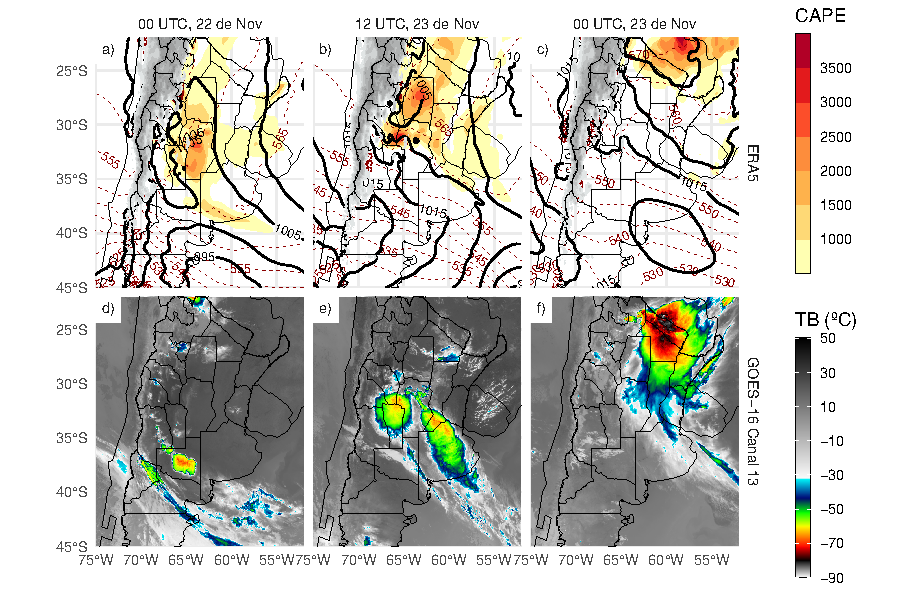
\includegraphics{thesis_files/figure-latex/caso-1} 

}

\caption{Presión a nivel del mar (hPa, contornos negros), espesor 1000-500 hPa (contornos rojos discontinuos) y energía potencial convectiva disponible (sombreada) según ERA5 y temperatura de brillo del canal 13 de GOES-16 para a,d) 00 y b,e) 12 UTC, 22 de Nov y c,f) 00 UTC, 23 de Nov.~}\label{fig:caso}
\end{figure}
\hypertarget{observaciones}{%
\section{Observaciones}\label{observaciones}}

Durante el periodo de estudio se realizaron diferentes experimentos para evaluar el impacto de diferentes fuentes de observaciones, entre los que se incluyen datos convecionales oficiales de superficie y altura, redes privadas de estaciones meteorológicas automáticas de superficie, vientos derivados de satelite, y radianzas en cielo claro. También se utilizaron observaciones para cuantificar la calidad de los análisis y pronósticos.

\hypertarget{conjuntos-de-observaciones-asimiladas}{%
\subsection{Conjuntos de observaciones asimiladas}\label{conjuntos-de-observaciones-asimiladas}}

\hypertarget{convencionales}{%
\subsubsection{Convencionales}\label{convencionales}}

Las observaciones convencionales (EMC) utilizadas forman parte del flujo de datos del Sistema Global de Asimilación de Datos (GDAS). Se asimilarán las observaciones convencionales incluidas en los archivos Binary Universal Form for Representation of Meteorological Data (PREPBUFR) generados por NCEP. Los archivos PREPBUFR incluyen observaciones de superficie procedentes de 117 estaciones meteorológicas de superficie (EMS), barcos, y observaciones de altura procedentes de 13 sitios de lanzamiento de radiosondeos y aviones dentro del área en estudio. Los triángulos naranjas de la Figura \ref{fig:dominio}a indican la ubicación de las estaciones de superficie incluidas en este experimento. La frecuencia de estas observaciones varia entre 1 hora para las estaciones de superficie y 12/24 horas para las radiosondas. Las observaciones del viento en superficie sobre los océanos (ASCATW) proceden de los dispersómetros y también se incluyen en los archivos PREPBUFR.

La tabla \ref{tab:tabla-obs} enumera todos los tipos de observación (presión en superficie, temperatura, humedad específica y viento) disponibles para cada fuente de observación, junto con el error asociado para cada una definidos de acuerdo a la configuración por defecto del sistema de asimilación usado en este trabajo. En algunos casos, el error varía con la altura y depende de la plataforma específica (avión y viento derivado del satélite). En cuanto al control de calidad aplicado a las observaciones convencionales, el sistema de asimilación realiza una primera comparación entre la innovación (la diferencia entre la observación y la observación simulada por el modelo para el campo preliminar) y un umbral predefinido que depende del error de observación (también incluido en la Tabla \ref{tab:tabla-obs}).

\hypertarget{ema}{%
\subsubsection{Red de Estaciones Meteorológicas Automáticas}\label{ema}}

También se asimilaron observaciones de 866 Estaciones Meteorológicas Automáticas (EMA) que forman parte de 17 redes de superficie públicas y privadas en la región. El conjunto de datos utilizado en este estudio fue obtenido del repositorio de datos de RELAMPAGO (Garcia et al., 2019). Estas estaciones se indican como cuadrados verdes en la Figura \ref{fig:dominio}a. Tienen mayor cobertura espacial que las EMC y una frecuencia de muestreo de 10 minutos en la mayoría de los casos. Todas las estaciones miden temperatura, pero sólo 395 estaciones proporcionan humedad, 422 la presión y 605 el viento.
Los errores de observación utilizados para asimilar estas observaciones son los mismos que para las observaciones de EMC (véase la tabla \ref{tab:tabla-obs}).

\hypertarget{vientos-estimados-por-satuxe9lite}{%
\subsubsection{Vientos estimados por satélite}\label{vientos-estimados-por-satuxe9lite}}

Las observaciones de viento derivadas de los satélites también se incluyen en los archivos PREPBUFR disponibles cada 6 hs, y consisten en estimaciones de GOES-16 (utilizando los canales visible, infrarrojo y de vapor de agua) y METEOSAT 8 y 11 (utilizando los canales visible y de vapor de agua). Estos satélites son geoestacionarios y tienen una frecuencia de escaneo de 15 minutos, por lo que, ante la presencia de nubosidad para estimar el viento, generarán estimaciones que estarán diponibles en cada ciclo de asimilación. Las observaciones de viento derivadas de los satélites METEOSAT tienen una resolución de 3 km mientras que las de GOES-16 tienen una resolución de 10 km. Debido al dominio elegido y la cobertura de estos satélites, GOES-16 es la principal fuente de observaciones de vientos derivados de los satélites (99 \% de las observaciones). Los errores de observación utilizados para asimilar estas observaciones siguen la configuración por defecto del GSI y se indican en la Tabla \ref{tab:tabla-obs}.
\begin{table}

\caption{\label{tab:tabla-obs}Características de las observaciones asimiladas: El código de cada tipo de observación y su fuente, las variables disponibles, el error de observación y los umbrales de control de calidad utilizados.}
\centering
\fontsize{9}{11}\selectfont
\begin{tabular}[t]{>{\raggedright\arraybackslash}p{4.5em}>{\raggedright\arraybackslash}p{5.5em}>{\raggedright\arraybackslash}p{6em}>{\raggedright\arraybackslash}p{8em}>{\raggedright\arraybackslash}p{8em}}
\toprule
Código & Plataforma & Variable & Error & Umbral de error\\
\midrule
 &  & Pressure & 1-1.6 $hPa^*$ & 3.6 $hPa$\\

 &  & Temperature & 1.5 $K$ & 7 $K$\\

 &  & Specific humidity & 20 \% & 8 $gKg^{-1}$\\

\multirow{-4}{4.5em}{\raggedright\arraybackslash CSWS   AWS} & \multirow{-4}{5.5em}{\raggedright\arraybackslash Surface weather stations} & Wind & 2.2 $ms^{-1}$ & 6 $ms^{-1}$\\
\cmidrule{1-5}
 &  & Pressure & 1.1-1.2 $hPa^{**}$ & 4 $hPa$\\

 &  & Temperature & 0.8-1.5 $K^*$ & 8 $K$\\

 &  & Specific humidity & 20 \% & 8 $gKg^{-1}$\\

\multirow{-4}{4.5em}{\raggedright\arraybackslash ADPUPA} & \multirow{-4}{5.5em}{\raggedright\arraybackslash Radiosondes} & Wind & 1.4-3 $ms^{-1}$* & 8 $ms^{-1}$\\
\cmidrule{1-5}
 &  & Temperature & 1.47-2.5 $K^+$ & 7 $K$\\

\multirow{-2}{4.5em}{\raggedright\arraybackslash AIRCFT} & \multirow{-2}{5.5em}{\raggedright\arraybackslash Aircrafts} & Wind & 2.4-3.6 $ms^{-1+}$ & 6.5-7.5 $ms^{-1+}$\\
\cmidrule{1-5}
ASCATW & Advanced Scatterometers & Wind & 1.5 $ms^{-1}$ & 5 $ms^{-1}$\\
\cmidrule{1-5}
 &  & Pressure & 1.3 $hPa$ & 4 $hPa$\\

 &  & Temperature & 2.5 $K$ & 7 $K$\\

 &  & Specific humidity & 20 \% & 8 $gKg^{-1}$\\

\multirow{-4}{4.5em}{\raggedright\arraybackslash SFCSHP} & \multirow{-4}{5.5em}{\raggedright\arraybackslash Ships and Buoys} & Wind & 2.5 $ms^{-1}$ & 5 $ms^{-1}$\\
\cmidrule{1-5}
SATWND & Satellite-derived winds & Wind & 3.8-8 $ms^{-1*+}$ & 1.3-2.5 $ms^{-1+}$\\
\bottomrule
\multicolumn{5}{l}{\rule{0pt}{1em}\textsuperscript{*} El error de la observación varía con la altura.}\\
\multicolumn{5}{l}{\rule{0pt}{1em}\textsuperscript{**} Observationes por encima de 600 hPa son rechazadas.}\\
\multicolumn{5}{l}{\rule{0pt}{1em}\textsuperscript{+} El error de la observación depende del tipo de reporte.}\\
\end{tabular}
\end{table}
\hypertarget{radiancias-de-satuxe9lite}{%
\subsubsection{Radiancias de satélite}\label{radiancias-de-satuxe9lite}}

En este trabajo se utilizaron radiancias de satélites disponibles a través del flujo de datos del GDAS, que incluye observaciones en el espectro infrarrojo y microondas. Dado que el dominio regional que se utilizará en este trabajo se encuentra en latitudes medias y que la mayoría de los satélites de interés están en órbitas polares, cada sensor escanea la zona sólo dos veces al día con una cobertura espacial que depende de la franja de cobertura satélite. Por esta razón, el número de observaciones de los satélites polares varía significativamente en cada ciclo de asimilación. En particular, los sensores multiespectrales proporcionaron entre 100 y 1000 observaciones por cada escaneo cada 12 horas, contribuyendo al 88 \% de la cantidad total de radiancias asimiladas (Tabla \ref{tab:table-rad}) en los experimentos descriptos en la sección \ref{config}. También se utilizó el satélite geoestacionario GOES-16 que tienen una frecuencia temporal de 15 y una resolución espacial de 2 kilómetros. En particular se utilizaron observaciones del sensor \emph{Advanced Baseline Imager} (ABI) que aporta más observaciones que el conjunto de satélites polares utilizados.
\begin{table}

\caption{\label{tab:table-rad}Lista de los sensores disponibles cada plataforma, el número de canales aceptados para su asimilación y el porcentaje de observaciones asimiladas calculado sobre todas las observaciones de radiancias y todos los ciclos de asimilación correspondientes al experimento RAD.}
\centering
\fontsize{9}{11}\selectfont
\begin{tabu} to \linewidth {>{\raggedright}X>{\raggedright}X>{\raggedleft}X>{\raggedright}X}
\toprule
Sensor & Plataforma & Canales asimilados & Porcentaje sobre el total\\
\midrule
AIRS & AQUA & 52 & 31.63 \%\\
\cmidrule{1-4}
 & NOAA15 & 2 & 3.31 \%\\
\cmidrule{2-4}
 & NOAA18 & 2 & 4.45 \%\\
\cmidrule{2-4}
\multirow[t]{-3}{*}{\raggedright\arraybackslash AMSUA} & METOP-A & 2 & 2.08 \%\\
\cmidrule{1-4}
 & METOP-A & 66 & 52.72 \%\\
\cmidrule{2-4}
\multirow[t]{-2}{*}{\raggedright\arraybackslash IASI} & METOP-B & 68 & 3.47 \%\\
\cmidrule{1-4}
 & NOAA19 & 2 & 0.68 \%\\
\cmidrule{2-4}
 & METOP-A & 3 & 0.8 \%\\
\cmidrule{2-4}
\multirow[t]{-3}{*}{\raggedright\arraybackslash MHS} & METOP-B & 3 & 0.85 \%\\
\bottomrule
\end{tabu}
\end{table}
Los sensores microondas disponibles para ser asimilados en el periodo de interés son el \emph{Advanced Microwave Sounding Unit - A} (AMSU-A) a bordo de las plataformas NOAA-15, NOAA-18 y METOP-A, y el \emph{Microwave Humidity Sounder} (MHS) a bordo de las plataformas NOAA-19, METOP-A y METOP-B.

AMSU-A ({\textbf{???}}) es un radiómetro de microondas que cuenta con 15 canales de observación diferentes entre 23.8 - 89 GHz y ha demostrado ser un importante sensor para el sondeo de la temperatura atmosférica (English et al., 2000). Cada canal detecta la radiación de microondas procedente de capas discretas de la atmósfera terrestre, la cual se describe mediante la función de peso, que corresponde la derivada de la transmitancia con respecto a la altura. El AMSU-A es conocido como un ``sensor de temperatura'' ya que sus canales fueron seleccionados para detectar la radiación emitida por capas sucesivas de la atmósfera. La Figura \ref{fig:wf}a muestra las funciones de peso en cielo claro para aquellos canales del AMSU-A que tienen sensibilidad en la tropósfera. No se incluyen en la asimilación de observaciones los dos primeros canales ubicados en 23.8 y 31.4 GHz ya que estos son sensibles a la fase líquida de las nubes y a la emisividad de la superficie, aunque si aportan información para el control de calidad de las observaciones de otros canales.


\begin{figure}

{\centering 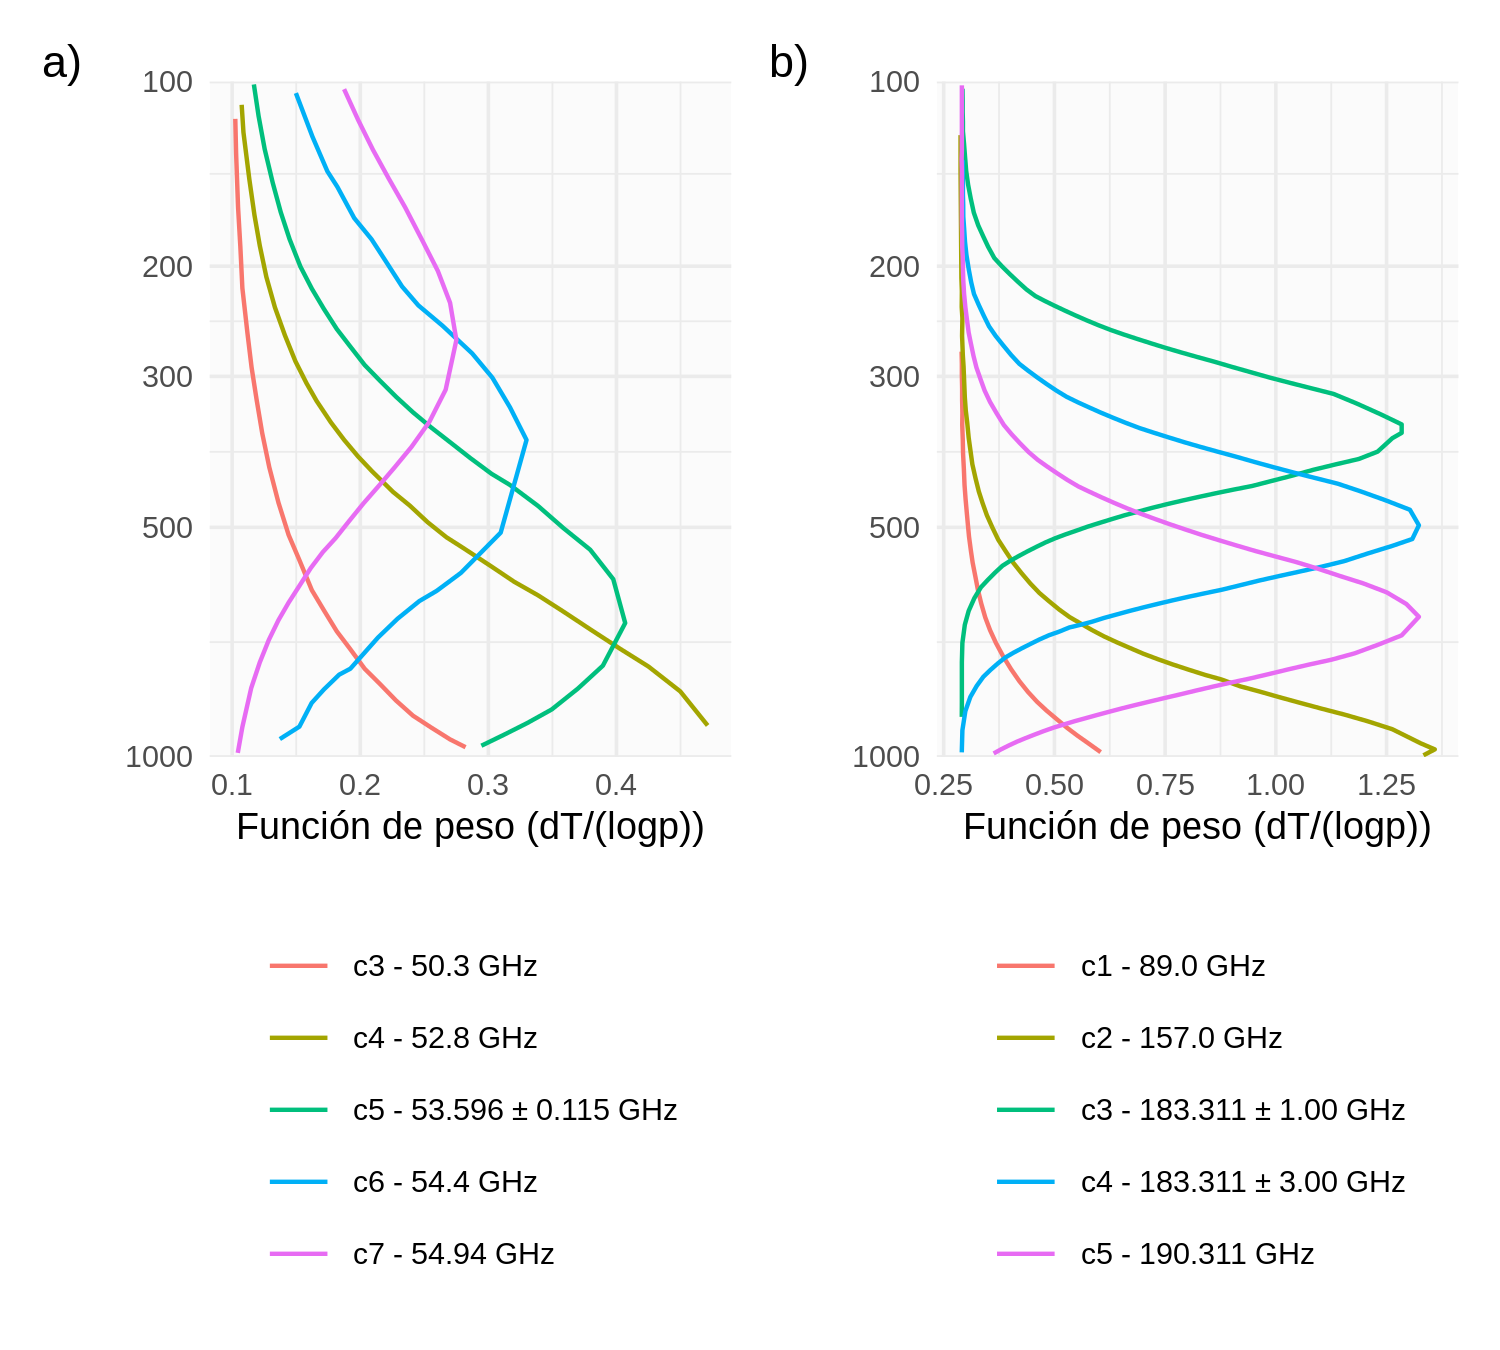
\includegraphics{thesis_files/figure-latex/wf-1} 

}

\caption{Funciones de peso calculada sobre cielo claro para distintos censores. a) AMSU-A, canal 3 - 50.3 GHz, canal 4 - 52.8 GHz, canal 5 - 53.596 \(\pm\) 0.115 GHz, canal 6 - 54.4 GHz, canal 7 - 54.94 GHz; MHS, canal 1 - 89.0 GHz, canal 2 - 157.0 GHz, canal 3 - 183.311 \(\pm\) 1.00 GHz, canal 4 - 183.311 \(\pm\) 3.00 GHz, canal 5 - 190.311 GHz; ABI, canal 8 - 6.2 \(\mu m\), canal 9 - 6.9 \(\mu m\), canal 10 - 7.3 \(\mu m\).}\label{fig:wf}
\end{figure}
Por ejemplo, la función de peso del canal 7 (54.94 GHz) muestra que la contribución máxima a la radiación de microondas detectada por el instrumento AMSU-A proviene de aproximadamente un altura de 10 km por encima de la superficie. Como indica la Tabla \ref{tab:table-rad} solo entre 2 y 4 canales del sensor AMSU-A se asimilaron en este trabajo. Esta selección de canales resulta de incluir sólo aquellos canales cuyo máximo en la función de peso se encuentra por debajo del tope del modelo utilizado (50 hPa) y que no son sensibles a la superficie terrestre y las nubes. Entre los canales asimilados se encuentran los canales 5 a 8 (53.596, 54.4, 54.94 y 55.5 GHz respectivamente).

De manera similar, el sensor microondas MHS es conocido por ser un ``sensor de humedad''. Este sensor tiene dos canales sensibles a la superficie y la presencia de nubes (canales 1 y 2: 89 y 157 GHz), y tres canales mayoritariamente sensibles al vapor de agua (canales 3, 4 y 5: 183.3 \(\pm\) 1.0, \(pm\) 3 y 190 GHz). Como indican las funciones de peso (Figura \ref{fig:wf}b), todos los canales del MHS se encuentran por debajo del tope del modelo, sin embargo, como se puede ver en la Tabla \ref{tab:table-rad}, entre 2 y 3 canales se asimilan en los experimentos llevados a cabo en esta tesis. Esto se debe a que en algunas situaciones el canal 5 se ve afectado por la presencia de nubes.

En cuanto a los sensores multiespectrales, se asimilaron dos: el \emph{Atmospheric Infrared Sounder} (AIRS) y el \emph{Infrared Atmospheric Sounding Interferometer} (IASI) ubicados en distintas plataformas (ver Tabla \ref{tab:table-rad}). IASI mide la radiación emitida por la Tierra en 8461 canales que cubren el intervalo espectral del infrarrojo térmico entre 645 y 2760 \(cm^{-1}\) (3.62 - 15.5 \(\mu m\)). De manera similar, AIRS tiene canales en 3 rangos del espectro electromagnético: 645 y 1136 \(cm^{-1}\), 1265 y 1629 \(cm^{-1}\), y 2169 y 2674 \(cm^{-1}\). Asimilar la totalidad de estos canales no es recomendable ya que tanto las observaciones como sus errores se encuentran muy correlacionados entre si, es por ello que numerosos estudios que se han enfocado en definir un conjunto de canales adecuado en el contexto de los pronósticos numéricos globales para su asimilación (por ejemplo, Collard (2007), Rabier et al. (2002)). Realizar un estudio de sensibilidad de los canales para la región de interés esta fuera del alcance de los objetivos de este trabajo, por lo que se decidió utilizar la configuración regional del sistema GSI en la cual se asimilan entre 52 y 68 canales distintos (ver Tabla \ref{tab:table-rad}).

Finalmente, en el caso de ABI, se asimilaron los canales sensibles al vapor de agua en distintos niveles, información que puede ser clave a la hora de pronosticar el desarrollo de convección húmeda profunda:
\begin{itemize}
\tightlist
\item
  Canal 8 (6.2 \(\mu m\)): vapor de agua en niveles altos
\item
  Canal 9 (6.9 \(\mu m\)): vapor de agua en niveles medios
\item
  Canal 10 (7.3 \(\mu m\)): vapor de agua en niveles bajos
\end{itemize}
La Figura \ref{fig:wf}c muestra las funciones de peso teóricas para una atmósfera estandar en latitudes medias para cada uno de estos canales. Si bien hay un solapamiento en las funciones de peso, el canal 8 es más sensible al vapor de agua alrededor de los 350 hPa, el canal 9 alrededor de 450 hPa y el canal 10 alrededor de los 600 hPa aproximadamente. En la sección \ref{canales} se analizará que combinación de canales da mejores resultados en el contexto de este caso de estudio.

\hypertarget{conjuntos-de-observaciones-para-verificaciuxf3n}{%
\subsection{Conjuntos de observaciones para verificación}\label{conjuntos-de-observaciones-para-verificaciuxf3n}}

Para evaluar el desempeño del sistema de asimilación de datos presentado en esta tesis, utilizamos los siguientes conjuntos de observaciones:
\begin{itemize}
\item
  \textbf{Datos horarios en niveles de presión de ERA5 (Hersbach et al., 2018):} Las variables de interés (temperatura del aire, humedad y viento) fueron interpoladas desde la reticula del reanalisis que tiene una resolución de 0.25\(^{\circ}\) a la retícula del modelo para compararlas con el análisis de cada experimento.
\item
  \textbf{Multi-Network Composite Highest Resolution Radiosonde Data (Earth Observing Laboratory, 2020):} radiosondeos en alta resolución lanzados desde varias ubicaciones durante el periodo de la campaña de campo RELAMPAGO en conjunto con las radiosondeos operativos del SMN. Sólo se utilizaron para la validación los sondeos que no ingresaron en el sistema de asimilación y que corresponden a los sitios de observación de la campaña. El periodo del experimento abarca las misiones \emph{Intensive Observation Period} (IOP) 7 (21/11/2018) y 8 (22/11/2018), durante las cuales se lanzaron 74 radiosondos en una pequeña zona cercana al centro del dominio experimental (Figura \ref{fig:dominio}b). Estas observaciones son de particular importancia ya que si bien corresponden a una región acotada del dominio, aportar información de alta resolución vertical y temporal ya que operacionalmente se lanzan sondeos una o dos veces al día.
\item
  \textbf{IMERG Final Run (Huffman et al., 2018):} estimación de la precipitación a partir de datos de la constelación de satelites GPM (por su nombre en inglés Global Precipitation Measurement) con una resolución espacial de 0,01\(^{\circ}\) y una resolución temporal de 30 minutos para validar la habilidad de los pronósticos de 1 hora para representar la precipitación sobre el dominio. La estimación de la precipitación se realiza combinando observaciones de sensores de microondas activos y pasivos que se complementa con estimaciones provenientes de sensores infrarojos a bordo de satélites polares.
\item
  \textbf{Datos del Sistema Nacional de Radares Meteorológicos (SINARAME):} Se utilizaron observaciones de radar para realizar una evaluación cualitativa y visual de la ubicacion e intensidad de la actividad convectiva. Los datos provienen de 9 radares ubicados en el dominio y son provistos por la red de radares Doppler de doble polarización en banda C (de Elía et al., 2017) con una frecuencia temporal de 10 minutos. Para este trabajo se utilizó únicamente la máxima reflectividad de la columna (COLMAX) más cercana al momento de análisis.
\item
  \textbf{Observaciones de las redes de estaciones meteorógicas automáticas:} Las observaciones de EMA descriptas en la sección \ref{ema} fueron utilizadas en la verificación de pronósticos inicializados a partir de los ánalisis generados. Estos pronósticos no incluyen asimilación de datos y por lo tanto estas observaciones son independientes y permiten evaluar calidad de los pronósticos en niveles bajos. s
\end{itemize}
\hypertarget{la-asimilaciuxf3n-de-datos}{%
\section{La asimilación de datos}\label{la-asimilaciuxf3n-de-datos}}

La asimilación de datos combina de manera optima un pronóstico numérico o campo preliminar en un tiempo \(t\) con las observaciones disponibles para ese mismo tiempo, generando un análisis (Carrassi et al., 2018). Esta combinación optima toma en cuenta el error asociado al modelo meteorológico (errores de pronóstico) y el error de las observaciones (que resulta de los errores instrumentales y los errores de representatividad) y su error será menor a los errores originales. Por esta razón el análisis es considerado desde un punto de vista estadistico y bajo ciertas hipotesis, como la \emph{mejor aproximación} disponible del estado real de la atmósfera.


\begin{figure}

{\centering 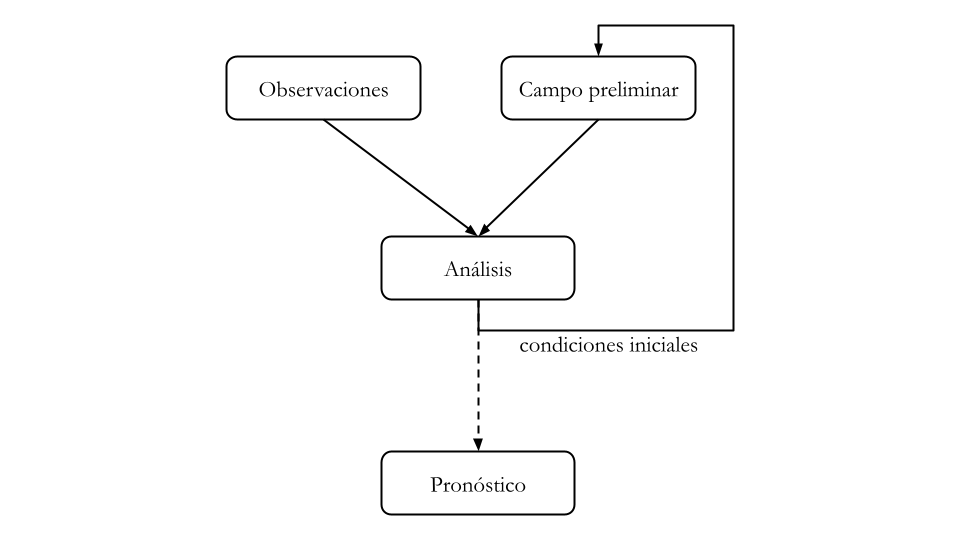
\includegraphics[width=1\linewidth,]{/home/paola.corrales/tesis_doctorado/figure/ciclo_asimilacion_teorico} 

}

\caption{Esquema de un ciclo de asimilación típico. El tiempo de las observaciones y el campo preliminar deberá coincidir.}\label{fig:ciclo-asimilacion-teorico}
\end{figure}
Un ciclo de asimilación de datos típico se muestra en la Figura \ref{fig:ciclo-asimilacion-teorico}. En un tiempo dado se comparan las observaciones disponibles con el campo preliminar para ese mismo tiempo, generando así el análisis que se utilizará como condición inicial para un futuro pronóstico o campo preliminar. En el caso de modelos globales, típicamente cada ciclo de asimilación de 6 horas utiliza el campo preliminar previo, es decir el pronóstico a 6 horas inicializado a partir del análisis anterior y las observaciones disponibles para las 6 horas previas o en un periodo similar centrado en la hora del análisis.

En este sentido tanto el modelo como las observaciones cumplen un rol fundamental en la asimilación. Por un lado las observaciones permiten incorporar información continua para corregir los pronósticos. Por el otro, el modelo permite \emph{transportar} información de regiones donde existe mucha información disponible (por ejemplo, los continentes) a regiones donde las observaciones son escasas (zonas oceánicas) manteniendo los balances físicos que rigen los procesos atmosféricos.

Existen distintas técnicas de asimilación de datos, cada una con sus ventajas y desventajas que fueron descriptas por Dillon (2017) en su tesis doctoral. En este trabajo, al igual que en trabajos previos en Argentina, se utilizará la técnica \emph{local ensemble transform Kalman filter} (LETKF, Hunt et al. (2007)) que forma parte de un conjunto de técnicas basadas en Filtros de Kalman por ensambles (Evensen, 2009). Los Filtros de Kalman utilizan el ensamble, un conjunto de pronósticos ligeramente diferentes que se resuelven simultaneamente para incluir los posibles estados de la atmósfera y provee información dependiente de la dinámica durante la ventana de asimilación y estimar el error del modelo a lo largo del tiempo.

En el contexto de los Filtros de Kalman, el análisis o \(x_a\) será el estado más probable de la atmósfera teniendo en cuenta las \(m\) observaciones \(y_o\) disponibles en un tiempo \(t\). Para poder comparar y combinar el campo preliminar con las observaciones, este es interpolado a la ubicación de las observaciones. En determinados casos, por ejemplo cuando se trabaja con observaciones de satélite o radar, será necesario transformar las variables del modelo (ej. temperatura y humedad) para obtener las variables observadas (ej. temperatura de brillo). En la siguiente ecuación \(H\) es el operador de las observaciones no lineal que se encarga de las interpolaciones y transformaciones necesarias sobre el campo preliminar \(x_f\), representado como un vector de dimensión \(n\).
\begin{equation}
x_a = x_f + K[y_o - H(x_b )]
\label{eq:eq1}
\end{equation}
La diferencia entre las observaciones \(y_o\) y el campo preliminar se denomina innovación. El análisis \(x_a\) se obtiene aplicando las innovaciones al campo preliminar pesadas por una matriz \(K\) o Ganancia de Kalman. Esta matriz de dimensión \(n\) x \(m\) que incluye información sobre los errores del pronóstico y de las observaciones como se observa en la ecuación \eqref{eq:eq3},
\begin{equation}
K = BH^T (HBH^T + R^{-1})^{-1}
\label{eq:eq3}
\end{equation}
donde \(B\) es la matriz de covarianza de los errores del pronóstico y \(R\) corresponde a la matriz de covarianza de los errores de las observaciones. La implementación de los los métodos de asimilación de datos suelen ser computacionalmente muy costosos, en parte debido a la estimación de la matriz \(B\).
\begin{equation}
\mathrm{ B \approx \frac{1}{m-1} \sum_{k=1}^{m}(x_{f}^{k}-\overline{x}_f)(x_{f}^{k}-\overline{x}_f)^T}
\label{eq:eq5}
\end{equation}
donde \(k \; \epsilon \; [1,m]\) es el miembro \emph{k-ésimo} del ensamble. Los métodos de Filtro de Kalman por Ensambles tienen la ventaja de estimar la matriz \(B\) a partir de ensamble y actualizarla en cada ciclo de asimilación para incluir los errores dependientes de la dinámica del sistema.
Esta estimación será buena si el ensamble logra capturar los posibles estados futuros o en otras palabras si la dispersión es sufiente para acompañar los cambios en la incertidumbre de los pronosticos a lo largo de los ciclos de asimilación. El ensamble debe, a su vez, ser capaz de capturar la inestabilidad en el sistema cuyos errores tienen tasas de crecimiento muy rápidas. Si esto ocurre la estimación de \(B\) será buena.

El método LETKF es una técnica eficiente ya que resuelve la ecuación \eqref{eq:eq1} en un espacio de dimensión reducida definido por los miembros del ensamble. Por lo tanto la matriz \(K\) no se resuelve explicitamente eliminando la necesidad de computar inversa de matrices. Cómo en el resto de los métodos que usan filtro de Kalman, se localiza o restringe el área de influencia de las observaciones a un determinado radio de localización reduciendo el costo computacional necesario. La localización tiene además otra ventajas. Por un lado, y desde el punto de vista dinámico las inestabilidades en la atmósfera son de naturaleza local y por lo tanto el tamaño del ensamble necesario para representar estas inestabilidades será menor que si miramos el problema globalmente (Patil et al., 2001). Por otro lado la localización evita la generación de covarianzas espureas entre observaciones que están alejadas entre si y son independientes reduciendo el ruido estádistico en la estimación del análisis. Además, este método calcula el análisis para cada punto de retícula individualmente, incorporando todas las observaciones que puedan tener influencia en ese punto al mismo tiempo permitiendo paralelizar los cálculos. De esta manera este método es hasta un orden de magnitud más rápido comparado con otros métodos desarrollados previamente (Whitaker et al., 2008).

\hypertarget{el-sistema-de-asimilaciuxf3n-gsi}{%
\subsection{El sistema de asimilación GSI}\label{el-sistema-de-asimilaciuxf3n-gsi}}

GSI por su nombre en inglés Gridpoint Statistical Interpolation, es un sistema de asimilación de datos de última generación, desarrollado inicialmente por el Environmental Modeling Center (EMC) del NCEP. Se diseñó como un sistema 3DVAR tradicional aplicado en el espacio de puntos de retícula de los modelos para facilitar la implementación de covarianzas anisotrópicas no homogéneas (Wu et al., 2002; Purser et al., 2003b, 2003a).
Está diseñado para funcionar en varias plataformas computacionales, crear análisis para diferentes modelos numéricos de pronóstico, y seguir siendo lo suficientemente flexible como para poder manejar futuros desarrollos científicos, como el uso de nuevos tipos de observación, una mejor selección de datos y nuevas variables de estado (Kleist et al., 2009).

Este sistema 3DVAR sustituyó al sistema de análisis operativo regional de punto de retícula del NCEP por el Sistema de Predicción de Mesoescala de América del Norte (NAM) en 2006 y al sistema de análisis global Spectral Statistical Interpolation (SSI) usado para generar las condiciones iniciales del Global Forecast System (GFS) en 2007 (Kleist et al., 2009).
En los últimos años, GSI ha evolucionado para incluir varias técnicas de asimilación de datos para múltiples aplicaciones operativas, incluyendo 2DVAR (por ejemplo, el sistema Real-Time Mesoscale Analysis (RTMA); Pondeca et al. (2011)), la técnica híbrida EnVar (por ejemplo los sistemas de asimilación de datos para el GFS, el Rapid Refresh system (RAP), el NAM, el HWRF, etc.), y 4DVAR (por ejemplo, el sistema de asimilación de datos para el Sistema Goddard de Observación de la Tierra, versión 5 (GEOS-5) de la NASA; Zhu and Gelaro (2008)).
GSI también incluye un enfoque híbrido 4D-EnVar que actualmente se utiliza para la generación del GFS.

Además del desarrollo de técnias híbridas, GSI permite el uso métodos de asimilación por ensambles. Para lograr esto, utiliza el mismo operador de las observaciones que los métodos variacionales para comparar el campo preliminar con las observaciones.
De esta manera los exaustivos controles de calidad desarrollados para los métodos variacionales también son aplicados en la asimilación por ensambles.
El código EnKF fue desarrollado por el Earth System Research Lab (ESRL) de la National Oceanic and Atmospheric Administration (NOAA) en colaboración con la comunidad científica.
Contiene dos algoritmos distintos para calcular el incremento del analisis, el serial Ensemble Square Root Filter (EnSRF, Whitaker and Hamill (2002)) y el Local Ensemble Kalman Filter (LETKF, Hunt et al. (2007)) aportado por Yoichiro Ota de la Agencia Meteorológica Japonesa (JMA).

Para reducir el impacto de covarianzas espurias en el incremento que se aplica al análisis, los sistemas por ensamble aplican una localización a la matriz de covarianza de los errores de las observaciones \(R\) tanto en la dirección horizontal como vertical.
GSI usa un polinomio de orden 5 para reducir el impacto de cada observación de manera gradual hasta llegar a una distancia límite a partir de la cual el impacto es cero. La escala de localización vertical se define en términos del logarítmo de la presión y la escala horizontal usualmente se define en kilómetros.
Estos parámetros son importantes a la hora de obtener un buen análisis y dependen de factores como el tamaño del ensamble y la resolución del modelo. La configuración utilizada para los experimentos de esta tesis se describe en la sección \ref{configmodelo}.

A su vez utiliza el Community Radiative Transfer Model (CRTM, Han et al. (2006)) como operador de las observaciones de radiancias que calcula la temperatura de brillo simulada por el modelo para poder compararlo con las observaciones de sensores satelitales.
GSI, además implementa un algoritmo de corrección de bias de las observaciones de radiancias de satélites.
La estimación hecha por el campo preliminar obtenida con el CRMT se compara con las observaciones de radiancia para obtener la innovación.
Esta innovación a su vez se utiliza para actualizar los coeficientes que permiten estimar el bias de las observaciones que se utilizá para obtener una innovación actualizada. Este proceso puede repetirse varias veces hasta que la innovación y los coeficientes de corrección de bias converjan.
Este algoritmo se describe en mayor detalle en la Sección \ref{sat}.

\hypertarget{el-modelo-de-transferencia-radiativa-crtm}{%
\subsubsection{El modelo de transferencia radiativa CRTM}\label{el-modelo-de-transferencia-radiativa-crtm}}

El Community Radiative Transfer Model (CRTM, Liu et al. (2008)) es un modelo de transferencia radiativa rápido que fue desarrollado conjuntamente por el NOAA Center for Satellite Applications and Research y el Joint Center for Satellite Data Assimilation (JCSDA). Es un modelo utilizado ampliamente por la comunidad de sensoramiento remoto ya que esdees de código abierto y se encuentra disponible para su uso públicamente. Se utiliza para la calibracion de instrumentos satelitales (Weng et al., 2013; Iacovazzi et al., 2020; Crews et al., 2021), y a su vez para generar retrievals a partir de observaciones satelites (Boukabara et al., 2011; Hu et al., 2019; Hu and Han, 2021). De especial importancia para este trabajo, es utilizado como operador de observaciones en la asimilacion de radianzas satelitales {[}Tong et al. (2020); barton2021{]}.

El CRTM es capaz de simular radiancias de microondas, infrarrojas y visibles utilizando perfiles atmosféricos de presión, temperatura, humedad y otras especies como el ozono. Recientemente Cutraro et al. (2021) evaluaron su despeño en la region con buenos resultados en la simulación de observaciones de GOES-16.

El CRTM es un modelo de transferencia radiativa \emph{``sensor-based''}, es decir que contiene parameterizaciones y tablas de coefficientes precalculadas especificamente para los sensores operativos. El CRTM se utiliza ampliamente para la asimilación de datos satelitales tanto microondas e infrarrojos. Incluye módulos que calculan la radiación térmica medida por satélite a partir de la absorción gaseosa, la absorción y dispersión de la radiación por aerosoles y nubes, y la emisión y reflexión de la radiación por la superficie terrestre. La entrada al CRTM incluye variables de estado atmosférico -por ejemplo, temperatura, vapor de agua, presión y concentración de ozono en capas definidas por el usuario, y variables y parámetros de estado de la superficie, incluyendo la emisividad, la temperatura de la superficie y el viento.

El modelo forward del CRTM permite simular observaciones satelitales de radiancias a partir del estado de la atmósfera. Esto es necesario para la asimilación de radiancias pero también es utilizado para verificar la precisión y los errores de estas observaciones.

El cálculo de las observaciones simuladas tiene un costo computacional muy alto ya que requiere transporner un matriz de grandes dimensiones y la minimización de una función de costo. Esta matriz K se construye a partir de las derivadas parciales de las radiancias con respecto a parámetros geofísicos. CRTM permite hacer estos cálculos de manera rápida para que pueda usarse en contextos operacionales.

Para obtener resultados rápidos, CRTM aplica ciertas simplificaciones y aproximaciones a la hora de resolver la ecuación de transferencia radiativa. En primer lugar asume que la atmósfera terrestre está formada por capas plano-paralelas y homogeneas en equilibrio termodinámico y donde los efectos tridimensionales y de polarización pueden ser ignorados.

En contextos de cielos despejados, además se asume que no existe dispersión y solo se considera la absorción de los gases en la atmósfera. En cielos nubosos y canales en el infrarrojo también se asume que no existe dispersión. Sin embargo, en el caso de canales de microondas la dispersión generada por las nubes es incluida. En este caso la ecuación de transferencia radiativa no se puede resolver anaíticamente y se recurre a modelos numéricos.

\hypertarget{sat}{%
\subsubsection{Asimilación de radiancias en GSI}\label{sat}}

El preprocesamiento y control de calidad de los datos es un paso esencial en la asimilación de radiancias y depende de cada sensor y canal. Esto incluye principalemnte un \emph{thinning} especial, la correcion del bias, y en particular en este estudio la deteccion de observaciones de cielos nubosos. Primero se aplicó un thinning espacial. Durante el proceso de thinning las observaciones que se van a asimilar se eligen en función de su distancia a los puntos de la retícula del modelo, la calidad de la observación (basada en la información disponible sobre la calidad de los datos) y el número de canales disponibles (para el mismo píxel y sensor) que han pasado el control de calidad. Además, el algoritmo de thnning prefiere las observaciones sobre el mar a las de la tierra o nieve (Hu et al., 2018). El objetivo al aplicar thinning es evitar incorporar información de procesos de escalas menores a las que puede representar el modelo.

Luego del thinning, se aplica la corrección de bias. La metodología de corrección de bias implementada en GSI tiene una componente dependiente de características termodinámicas del aire y otro dependiente del ángulo de escaneo (Zhu et al., 2014) y se calcula como una polinomio lineal de N predictores \(p_i(x)\), con coeficientes asociados \(\beta_i\). Por lo tanto, la temperatura de brillo corregida por bias (\(BT_{cb}\)) puede obtenerse como
\begin{equation}
\mathrm{\mathit{BT_{cb}} =\mathit{ BT} + \sum_{i = 0}^{N} \beta_i p_i (x)}
\label{eq:eq12}
\end{equation}
GSI tiene un término de corrección de bias constante (\(p_0 = 1\)) mientras que los términos restantes y sus predictores son el contenido de agua líquida de las nubes (CLW), la tasa de cambio de temperatura con la presión, el cuadrado de la tasa de y la sensibilidad de la emisividad de la superficie. El bias dependiente del ángulo de escaneo se modela como un polinomio de 4\(^\circ\) orden (Zhu et al., 2014).

En el sistema GSI, los coeficientes \(\beta_i\) se entrenan utilizando un método de estimación variacional que genera los \(\beta_i\) que proporciona el mejor ajuste entre la simulación y las observaciones.

La metodología detección de pixeles nubosos depende de la longitud de onda de las observaciones. Para las radiancias de microondas, las observaciones potencialmente contaminadas por nubes se detectan utilizando los índices de dispersión y del Liquid Water Path (LWP) calculados a partir de diferencias entre distintos canales de cada sensor (Zhu et al., 2016; Weston et al., 2019). Para los canales infrarrojos, las observaciones contaminadas por nubes se detectan utilizando el perfil de transmitancia calculado por el modelo CRTM. Además, GSI comprueba la diferencia entre las observaciones y la temperatura de brillo simulada para detectar los píxeles nublados. Un caso particular son las las observaciones de ABI ya que se utiliza la mascara de nubes que se genera como producto de nivel 2 y que está disponible con la misma resolución que las observaciones. Esta máscara de nubes se genera combinando información de 8 canales del sensor ABI desde el punto de vista espacial y temporal.

Por otro lado, el control de calidad de GSI filtra aquellas observaciones de canales cercanos al rango visible sobre superficies de agua con un ángulo cenital mayor a 60\(^{\circ}\) para rechazar aquellas observaciones que pudieran estar contaminadas por reflexión. Para las observaciones en el infrarrojos y microondas también realiza una chequeo de la emisividad para detectar observaciones contaminadas por efecto de la superficie.

Finalmente se aplica un \emph{gross check}, es decir, se compara la diferencia entre la observación y la observación simulada por el modelo y un umbral predefinido que depende del error de observación para rechazar observaciones erroneas. La ubicación vertical de cada observación de radiancia se estimó como el nivel del modelo en el que se maximizaba su función de peso calculada por el CRTM. La función de peso de cada canal corresponde al cambio en la transmitancia con la altura y su máximo describe la capa de la atmósfera desde donde la radiación captada por el canal fue emitida. Los sensores multiespectrales tienen una buena cobertura vertical y son capaces de captar desde la baja troposfera hasta la baja estratosfera. Los canales elegidos para la asimilación y sus errores asociados se definieron teniendo en cuenta la configuración que GSI para generar los análisis y pronósticos de GFS, el tope del modelo elegido en este trabajo (50 hPa) y la posible influencia de la superficie.

\hypertarget{configmodelo}{%
\section{Configuración del sistema de asimilación}\label{configmodelo}}

Las simulaciones numéricas que conforman los experimentos que se discuten en este trabajo se realizan utilizando la versión 3.9.1 de modelo WRF (Skamarock et al., 2008).
Se utilizó una resolución horizontal de 10 km y 37 niveles en la vertical con el tope del modelo en 50 hPa.
Las condiciones iniciales y de contorno surgen del análisis del Global Forecast System (GFS, resolución horizontal de 0,25\(^{\circ}\) y resolución temporal de 6 horas; National Centers for Environmental Prediction, National Weather Service, NOAA, U.S. Department of Commerce (2015)).
El dominio de 150 x 200 puntos de retícula cubre la zona indicada en la Figura \ref{fig:dominio} para capturar el desarrollo del SCM durante el periodo simulado.

Los análisis se generaron utilizando la implementación LETKF (V1.3, Hunt et al. (2007)) que forma parte del sistema de análisis Gridpoint Statistical Interpolation (GSI V3.8; Shao et al. (2016)).
Se utilizó un enfoque de actualización rápida con análisis horario y una ventana de asimilación centrada, lo que significa que se asimilaron todas las observaciones dentro de \(\pm\) 30 minutos del tiempo de análisis.
Además, las observaciones se asimilaron usando un enfoque 4D, es decir, comparándolas con el first guess más cercano disponible con una frecuencia de 10 minutos.
Para las observaciones de satelite, se utilizó el Community Radiative Transfer Model versión 2.3 (CRTM; Han et al. (2006)) como operador de observaciones para calcular las temperaturas de brillo simuladas por el modelo.

Utilizamos un conjunto de 60 miembros, cuya media al principio del ciclo de AD se inicializa utilizando el análisis deterministico del GFS al que se le suman perturbaciones aleatorias para generar el ensamble incial. Las perturbaciones se generaron como diferencias escaladas entre dos estados atmosféricos aleatorios obtenidos a partir de los datos del Reanálisis del Sistema de Predicción del Clima (CFSR) con una resolución horizontal de 0,5\(^{\circ}\) que tiene una evolución temporal suave (Necker et al., 2020; Maldonado et al., 2021). De este modo, preservamos el equilibrio casi hidrostático y geostrófico de las escalas mayores. Este método ayuda a evitar una subestimación del spread del ensamble (Ouaraini et al., 2015). Las perturbaciones también se aplicaron en los bordes laterales para mantener niveles adecuados de spread dentro del dominio del ensamble.

Además de las perturbaciones aleatorias en los bordes laterales, se utilizó un esquema de multifísicas para representar mejor la incertidumbre en el modelo dentro del sistema de AD. Utilizamos 9 configuraciones diferentes que consisten en la combinación de 3 esquemas de convección húmeda (Kain-Fritsch, Kain (2004); Grell-Freitas, Grell and Freitas (2013); y Betts-Miller-Janjic, Janjić (1994)) y 3 esquemas de capa límite planetaria (Esquema de la Universidad de Yonsei, Hong, Kim, et al. (2006); Esquema Mellor-Yamada-Janjic, Janjić (1994); y Mellor-Yamada Nakanishi Niino, Nakanishi and Niino (2009)). La distribución de estas parametrizaciones entre los 60 miembros del ensamble se muestra en la Tabla \ref{tab:miembros-desc}. Todos los miembros del ensamble utilizan las mismas parametrizaciones del modelo de superficie terrestre (Noah-MP, Chen and Dudhia (2001)), de microfísica (esquema de un solo momento de 6 clases del WRF, Hong, Noh, et al. (2006)) y de procesos radiativos (esquema de onda corta y onda larga del RRTMG, Iacono et al. (2008)).
\begin{table}

\caption{\label{tab:miembros-desc}Generación de los 60 miembros del ensamble multifísica como combinación de parametrizaciones de Cumulus y PBL}
\centering
\fontsize{9}{11}\selectfont
\begin{tabular}[t]{c>{\centering\arraybackslash}p{8em}>{\centering\arraybackslash}p{8em}>{\centering\arraybackslash}p{8em}}
\toprule
\multicolumn{1}{c}{ } & \multicolumn{3}{c}{PBL} \\
\cmidrule(l{3pt}r{3pt}){2-4}
Cumulus & MYJ & MYNN2 & YSU\\
\midrule
BMJ & 5, 14, 23, 32, 41, 50, 59 & 8, 17, 26, 35, 44, 53 & 2, 11, 20, 29, 38, 47, 56\\
GF & 6, 15, 24, 33, 42, 51, 60 & 9, 18, 27, 36, 45, 54 & 3, 12, 21, 30, 39, 48, 57\\
KF & 4, 13, 22, 31, 40, 49, 58 & 7, 16, 25, 34, 43, 52 & 1, 10, 19, 28, 37, 46, 55\\
\bottomrule
\end{tabular}
\end{table}
Para reducir el efecto de las correlaciones espurias en la estimación de las covarianzas de los errores de las observaciones, utilizamos un radio de localización horizontal de 180 km y un radio de localización vertical de 0,4 (en coordenadas del logaritmo de la presion ) como en Dillon et al. (2021) para todos los tipos de observaciones.
Se aplicó con un parámetro de inflación \(\alpha=0,9\) para mitigar el impacto de los errores de muestreo y para considerar los errores del modelo que no se tienen en cuenta en el enfoque mutifísica del ensamble (Whitaker and Hamill, 2012).


\begin{figure}

{\centering 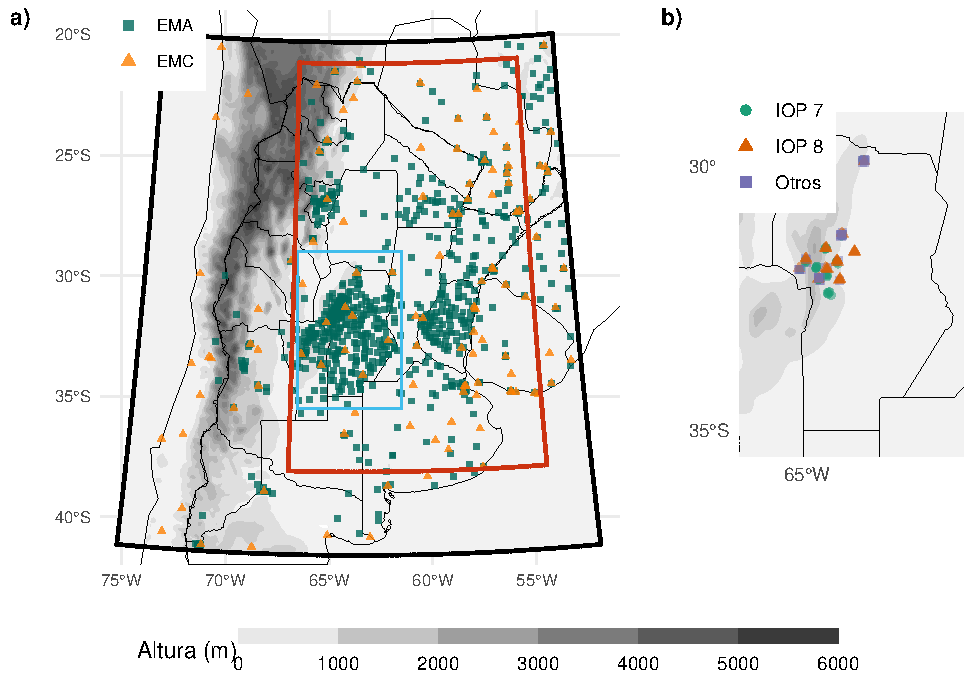
\includegraphics[width=0.8\linewidth,]{thesis_files/figure-latex/dominio-1} 

}

\caption{a) Dominio utilizado para las simulaciones (recuadro negro), dominio interior utilizado para la comparación entre experimentos (recuadro rojo), la región mostrada en b) (recuadro azul claro), y la ubicación de las Estaciones Meteorológicas Automáticas (EMA, cuadrados verdes) y las Estaciones Meteorológicas Convencionales (EMC, triángulos naranjas). b) Ubicación de los lanzamientos de radiosondeos durante RELAMPAGO. Los puntos verdes corresponden a los radiosondeos lanzados durante el IOP 7, los triángulos naranjas son radiosondeos lanzados durante el IOP 8, y los cuadrados morados son radiosondeos lanzados fuera de los periodos de medición intensiva. También se muestra la topografía en metros (sombreada).}\label{fig:dominio}
\end{figure}
Los errores de las observaciones utilizados fueron definidos de acuerdo a las tablas de errores disponibles como parte del sistema GSI. Para las observaciones de radiancias polares se aplicó un thinning con una retícula de 60 km siguiendo Singh et al. (2016), Jones et al. (2013) y Lin et al. (2017) ya utilizan configuraciones de modelo similares a la usada en este trabajo. Para las observaciones de GOES-16 se realizaron pruebas de sensibilidad para determinar la resolución de thinning más apropiada para este tipo de observaciones que se describen en la sección \ref{thinning}.

Los coeficientes de corrección de bias para las observaciones de satélites polares se inicializaron a las 18 UTC del 18 de noviembre de 2018 a partir los coeficientes generados para la misma hora por el sistema GFS. El sistema de asimilación se configuró para utilizar una varianza de error de los coeficientes constante de 0,01 para evitar grandes ajustes en los coeficientes estimados en cada momento. Por razones que se describen en la seccion \ref{asim-goes} se decidió no aplicar corrección de bias a las observaciones de GOES-16.

\hypertarget{muxe9todos-de-verificaciuxf3n}{%
\section{Métodos de verificación}\label{muxe9todos-de-verificaciuxf3n}}

Se seleccionaron un conjunto de métricas para evaluar diferentes aspectos del análisis obtenido para cada experimento y los pronósticos inicializados a partir de ellos. Estas métricas incluyen una validación de cómo se cuantifica la incertidumbre en el first guess y en el análisis, y cómo los diferentes experimentos se ajustan a un conjunto independiente de observaciones que no se asimilan.

Para evaluar la consistencia de la estimación de la incertidumbre en el first guess y en el análisis utilizamos la Reduced Centered Random Variable o RCRV (Candille et al. (2007)) que se define como:
\begin{equation}
\mathrm{RCRV} = \frac{m - x_o}{\sqrt{\sigma_o^2 + \sigma^2}}
\label{eq:eq6}
\end{equation}
donde \(x_o\) es la observación asimilada y su error \(\sigma_o\), \(m\) la media ensamble del análisis en el espacio de las observaciones, y la desviación estándar \(\sigma\) del ensamble
La media de \(RCRV\) calculada sobre todas las realizaciones representa el sesgo de la media del conjunto con respecto a las observaciones normalizadas por la incertidumbre estimada:
\begin{equation}
\mathrm{\mathit{mean RCRV} = E[RCRV]}
\label{eq:eq7}
\end{equation}
La desviación estándar de la \(RCRV\) o \(sd RCRV\) mide la concordancia de la dispersión del ensamble y el error de observación con respecto a la distancia entre la media del ensamble y las observaciones, y por lo tanto, la sobre o subdispersión sistemática del ensamble:
\begin{equation}
\mathit{sd RCRV} = \sqrt{\frac{1}{M -1}\sum_{i=1}^{M}(RCRV_i - \mathit{mean RCRV})^2}
\label{eq:eq8}
\end{equation}
donde \(M\) es el tamaño del ensamble. Suponiendo que el error de observación fue estimado con precisión, un \(sd RCRV > 1\) indica que el ensamble es subdispersivo (es decir, la distancia entre las observaciones y los pronósticos es mayor de lo esperado), y un \(sd RCRV < 1\) indica que el conjunto es sobredispersivo (es decir, la distancia entre las observaciones y los pronósticos es menor de lo esperado). Un sistema consistente no tendrá sesgo (\(media RCRV = 0\)) y una desviación estándar igual a 1 (\(sd RCRV = 1\)).

Para analizar el ajuste del first guess y el análisis a un conjunto de observaciones independientes se calculó la raiz del error cuadrático medio (RMSE) y el BIAS:
\begin{equation}
\mathit{RMSE} = \sqrt{\frac{1}{N}\sum_{i = 1}^{N} (X_i - O_i)^{2}}
\label{eq:eq9}
\end{equation}
\begin{equation}
\mathit{BIAS} = \frac{1}{N}\sum_{i = 1}^{N} (X_i - O_i)
\label{eq:eq10}
\end{equation}
donde \(X\) representa el modelo interpolado al espacio de la observaciones, \(O\) las observaciones independientes, y N es el tamaño de la muestra.

Para comparar la precipitación pronosticada por el first-guess con las estimaciones de precipitación de IMERG, calculamos el Fractions Skill Score (FSS, Roberts (2008)) para diferentes radios de influencia y umbrales de precipitación:
\begin{equation}
\mathrm{\mathit{FSS} = 1-\frac{\sum_{i=1}^{N} ({P_x}_i-{P_o}_i)^{2}}{\sum_{i=1}^{N} ({P_x}_i)^{2}+\sum_{i=1}^{N} ({P_o}_i)^{2}}}
\label{eq:eq11}
\end{equation}
donde \(P_{oi}\) es la proporción de puntos de reticula en el subdominio \(i-th\), definido por el radio de influencia, donde la que la precipitación acumulada observada es mayor que un umbral especificado. Siguiendo a Roberts et al. (2020), \(P_{xi}\) se calcula sobre el ensamble completo y cuantifica de la probabilidad de que la precipitación sea mayor al mismo umbral en cada punto de cuadrícula, y luego promediando sobre el subdominio \(i-th\).

Para los pronósticos por ensambles se calculó la probabilidad de precipitación por encima de determinados umbrales en cada punto de retícula como la proporción de miembros del ensamble que pronósticaron precipitación por encima de cada umbral. Además se generaron gráficos de confiabilidad (Wilks, 2011) con intervalos de probabilidades pronósticadas de 10\% para analizar la calibración de los pronósticos inicializados a partir de los análisis de cada experimento.

\hypertarget{recursos-computacionales}{%
\section{Recursos computacionales}\label{recursos-computacionales}}

Todos los experimentos corrieron en la supercomputadora Cheyenne del Centro Nacional de Investigación Atmosférica (NCAR) (Computational and Information Systems Laboratory, 2019). El posprocesamineto y análisis se realizó en {[}CIMA{]}. El análisis de datos se generó utilizando el lenguaje de programación R (R Core Team, 2020), utilizando los paquetes data.table (Dowle and Srinivasan, 2020) y metR (Campitelli, 2020), entre otros.
Todos los gráficos se han realizado con ggplot2 (Wickham, 2009) y la versión final de la tesis se generó con knitr, rmarkdown (Xie, 2015; Allaire et al., 2019) y tesisdown (Ismay and Solomon, 2022).

\hypertarget{ch1}{%
\chapter{Asimilacion de observaciones de estaciones meteorológicas automáticas, vientos derivados de satélite y radianzas de satelites polares}\label{ch1}}

Este capítulo busca contribuir a la cuantificación y comparación del impacto de asimilar observaciones de las estaciones meteorológicas automáticas de alta resolución, viento estimando por satélite y radiancias de cielo claro de satélites polares a la hora de aplicar la asimilación de datos para mejorar los pronósticos numéricos de eventos severos sobre Sudamérica, donde la red de observación convencional es bastante escasa y otras fuentes de información podrían potencialmente cubrir las áreas menos observadas y aportar información en las escalas más pequeñas.

\hypertarget{metodologuxeda}{%
\section{Metodología}\label{metodologuxeda}}

\hypertarget{config}{%
\subsection{Configuracion de los experimentos}\label{config}}

Para investigar el impacto de las diferentes observaciones en el análisis, se realizaron cuatro experimentos de asimilación de datos utilizando diferentes conjuntos de observaciones (Tabla \ref{tab:table-exp}). El experimento CONV utiliza únicamente las observaciones convencionales de PREPBUFR. En un segundo experimento, denominado AWS, se asimilan todas las observaciones incluidas en CONV más las observaciones de EMA con 10 minutos de frecuencia. En el tercer experimento, denominado SATWND, se asimilan las observaciones del experimento AWS junto con los vientos estimados por satélite. Por último, un cuarto experimento, denominado RAD, asimila todas las observaciones mencionadas previamente más las radiancias en cielo claro procedentes de los sensores a bordo de los satélites de órbita polar, como se describe en la sección \ref{sat}.
\begin{table}

\caption{\label{tab:table-exp}Tipos de observaciones asimiladas en cada experimento.}
\centering
\begin{tabu} to \linewidth {>{\raggedright\arraybackslash}p{8em}>{\centering\arraybackslash}m{2.5em}>{\centering\arraybackslash}m{2.5em}>{\centering\arraybackslash}m{3em}>{\centering\arraybackslash}m{3em}}
\toprule
Obs type & CONV & AWS & SATWND & RAD\\
\midrule
Convencional (PREPBUFR) & x & x & x & x\\
Convencional (EMA) &  & x & x & x\\
Viento estimado por satélite &  &  & x & x\\
Radiancias &  &  &  & x\\
\bottomrule
\end{tabu}
\end{table}

\begin{figure}
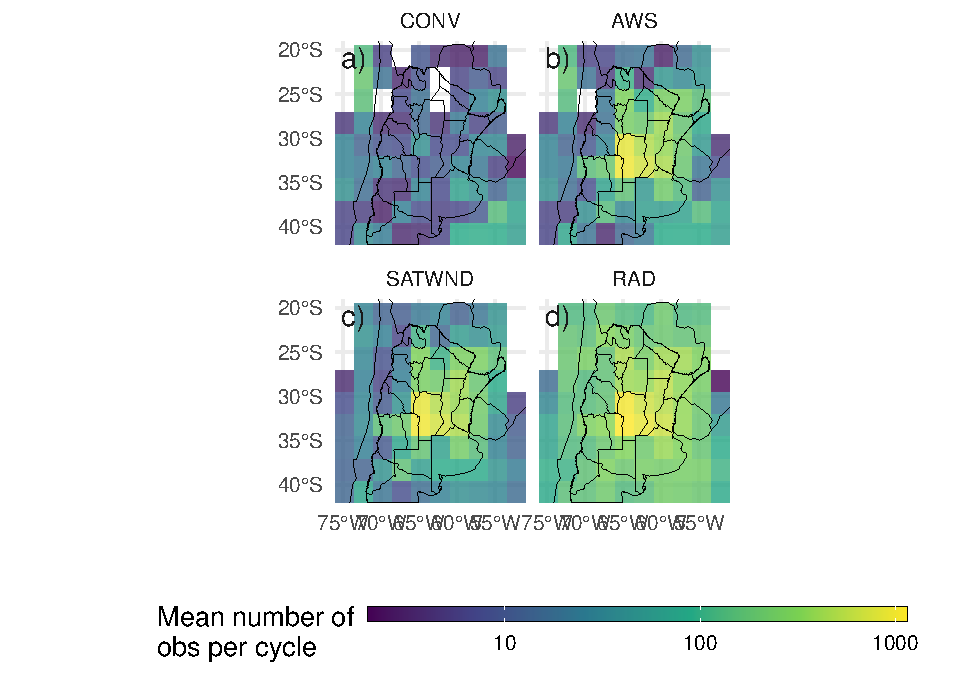
\includegraphics{thesis_files/figure-latex/obs-horizontal-1} \caption{Distribución espacial horizontal media de las observaciones disponibles en cada ciclo de asmilación para los experimentos a) CONV, b) AWS, c) SATWND y d) RAD calculados sobre cajas de 2,5\(^{\circ}\).}\label{fig:obs-horizontal}
\end{figure}

\begin{figure}
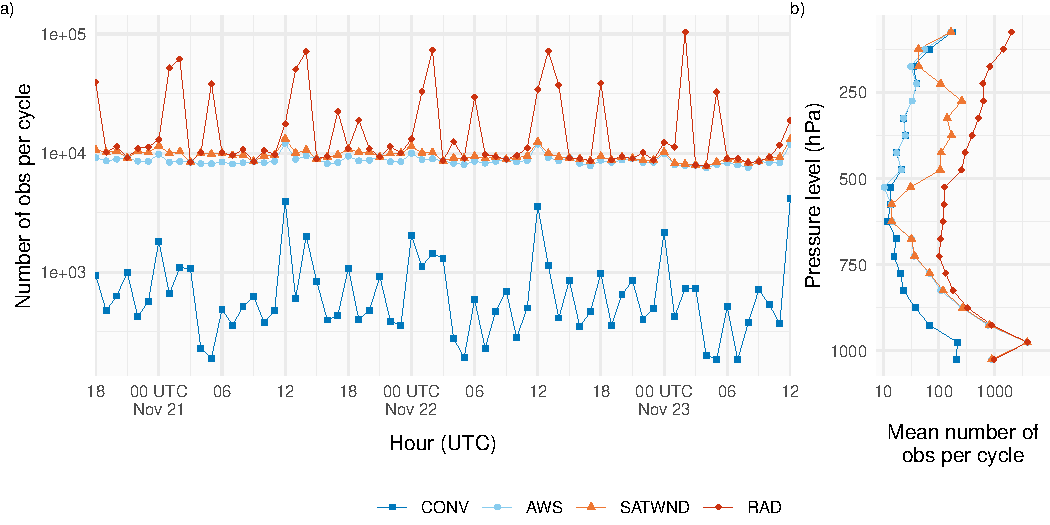
\includegraphics{thesis_files/figure-latex/obs-cycle-1} \caption{a) Número de observaciones asimiladas por ciclo y b) número medio de observaciones asimiladas por ciclo dividido en capas verticales de 50 hPa de espesor para los experimentos CONV (cuadrados azules), AWS (puntos celestes), SATWND (triángulos naranjas) y RAD (diamantes rojos).}\label{fig:obs-cycle}
\end{figure}
La distribución horizontal del promedio de observaciones asimiladas en cada ciclo de asimilación de cada experimento se muestra en la Figura \ref{fig:obs-horizontal}. El mayor número de observaciones asimiladas sobre el centro y el este del dominio corresponde a las observaciones de EMA. En la Figura \ref{fig:obs-cycle}a se muestra el número de observaciones asimiladas a lo largo del tiempo. Los máximos locales a las 12 y a las 00 UTC encontrados principalmente en CONV corresponden a las observaciones obtenidas con los sondeos operativos. La fuerte variabilidad en el número de observaciones de radiancias por ciclo es también notable y depende de la cobertura de cada satélite. Los máximos a las 13-14 y 01-02 UTC en RAD corresponden a la contribución de los sensores multiespectrales. La distribución vertical del número medio de observaciones por ciclo (Figura \ref{fig:obs-cycle}b) muestra un máximo en niveles bajos debido a las observaciones de EMA. Los vientos estimados por satélite tienen un máximo en la troposfera alta (entre 500-250 hPa). Por encima de 850 hPa, la mayoría de las observaciones corresponden a radiancias.

Todos los experimentos de asimilación comienzan a las 18 UTC del 20 de noviembre de 2018 y continúan hasta las 12 UTC del 23 de noviembre (un total de 67 horas/ciclos de asimilación). El ensamble inicial de 60 miembros se genera según se explica en la sección \ref{configmodelo} y todos los experimentos se inician con un periodo de spin up sin asimilación de observaciones entre las 12 UTC y las 18 UTC de Nov, 20 (Figura \ref{fig:cycle}).


\begin{figure}
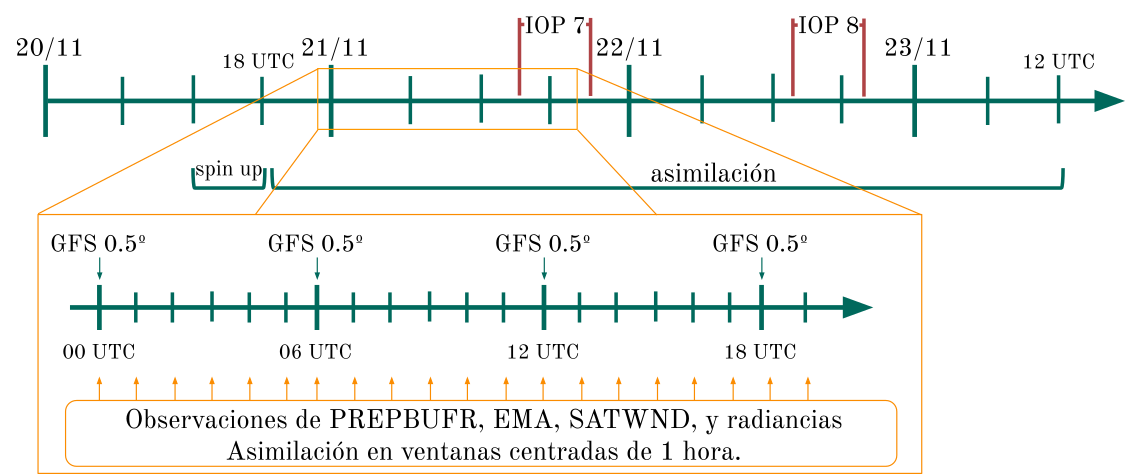
\includegraphics[width=1\linewidth,]{/home/paola.corrales/tesis_doctorado/figure/analisis} \caption{Diagrama de los ciclos de asimilación entre las 18 UTC del 20 de noviembre y las 12 UTC del 23 de noviembre más el periodo de spin up de 6 horas. La sección ampliada muestra la asimilación horaria que se realiza dentro de una ventana centrada de una hora y la incorporación de condiciones de borde del GFS cada 6 horas. Se muestran las dos misiones IOP de la campaña RELAMPAGO.}\label{fig:cycle}
\end{figure}
\hypertarget{resultados}{%
\section{Resultados}\label{resultados}}

\hypertarget{consistencia-del-ensamble}{%
\subsection{Consistencia del ensamble}\label{consistencia-del-ensamble}}

Para investigar la capacidad de la media del ensamble del first-guess para ajustarse a las observaciones teniendo en cuenta las incertidumbres del pronóstico y de las observaciones, se calcularo el \(meanRCRV\) y el \(sdRCRV\) para el experimento RAD. Como este experimento asimila todos los tipos de observaciones utilizados en este trabajo, es posible analizar la coherencia del ensamble comparándolo con cada tipo de observación. La figura \ref{fig:rcrv-sfc} muestra el \(sdRCRV\) para las observaciones de superficie promediadas en una retícula de 2,5°. El \(sdRCRV\) para las observaciones del viento (Figura \ref{fig:rcrv-sfc}a) es cercano a 1, lo que sugiere una buena concordancia entre la dispersión del ensamble, el error de pronóstico y el error de observación. Para la temperatura (Figura \ref{fig:rcrv-sfc}b), los resultados son similares, salvo que para algunas zonas del oeste del dominio donde el \(sdRCRV\) puede llegar a ser de 4,5. Estos valores más altos de \(sdRCRV\) pueden estar asociados a errores sistemáticos derivados de las diferencias entre la topografía del modelo y al altura a la que están ubicadas las observaciones. La circulación de pequeña escala asociada al terreno complejo podría no estar bien resuelta por el modelo podría contribuir a aumentar la distancia entre el pronóstico y las observaciones. Estos aspectos no suelen ser captados por la dispersión del ensamble, a menos que se utilice un esquema de inflación dependiente del espacio bien ajustado, lo que conduce a mayores valores de \(sdRCRV\).

La figura \ref{fig:rcrv-profile} muestra la media y el desvío estándar del RCRV para las observaciones de altura. Las figuras \ref{fig:rcrv-profile}a-b muestran las estadísticas de RCRV para los sondeos (ADPUPA) y aviones (AIRCAR y AIRCFT). Tanto ADPUPA como AIRCFT muestran, en general, un buen acuerdo entre la dispersión del ensamble y el error de observación. Como las observaciones de sondeo y sus errores asociados son considerados de buena calidad, este resultado indica que el ensamble tiene una dispersión adecuada. AIRCAR presenta un perfil irregular con valores \(sdRCRV\) que sugieren que el error de este tipo de observación está sobreestimado. ADPUPA y AIRCAR presentan un perfil de \(meanRCRV\) cercano a cero en los niveles medios y altos. En niveles bajos, el perfil \(meanRCRV\) es positivo, mostrando un bias cálido presente en el modelo, característica ya estudiada en Ruiz et al. (2010) y Dillon et al. (2021).

Las observaciones de vientos estimadas por satélites varían en número dependiendo del satélite y del nivel. En la Figura \ref{fig:rcrv-profile}c sólo se incluye el \(RCRV\) calculado con al menos 100 observaciones disponibles para cada sensor y nivel. En niveles bajos, donde no hay muchas observaciones disponibles, los perfiles de \(meanRCRV\) y \(sdRCRV\) muestran una mayor desviación del comportamiento esperado con un bias negativo, y una posible sobreestimación del error de observación. Las estimaciones del viento derivadas de los canales de vapor de agua son abundantes por encima de 500 hPa, donde su bias es cercano a cero. La única excepción son las observaciones de EUMETSAT que contribuyen muy poco en la región.

Los perfiles de \(meanRCRV\) calculados a partir de las observaciones de radiancias (Figura \ref{fig:rcrv-profile}d) no muestran casi ningún bias y lo mismo ocurre si se calcula el \(mean RCRV\) sobre cada canal de cada sensor (no incluido en el trabajo). Esto indica que el algoritmo de corrección del bias funciona como se esperaba. Los valores de \(sd RCRV\) son inferiores a 1 para todos los sensores, posiblemente debido a una sobreestimación de los errores de observación para reducir la influencia de las observaciones potencialmente erróneas.

En general, estos resultados indican que la dispersión del ensamble es coherente con el error de pronóstico a corto plazo y que los errores sistemáticos son relativamente pequeños para la mayoría de los tipos de observación utilizados en este trabajo. Además, estos resultados sugieren que el parámetro de inflación \(\alpha = 0,9\) es adecuado para el sistema.


\begin{figure}
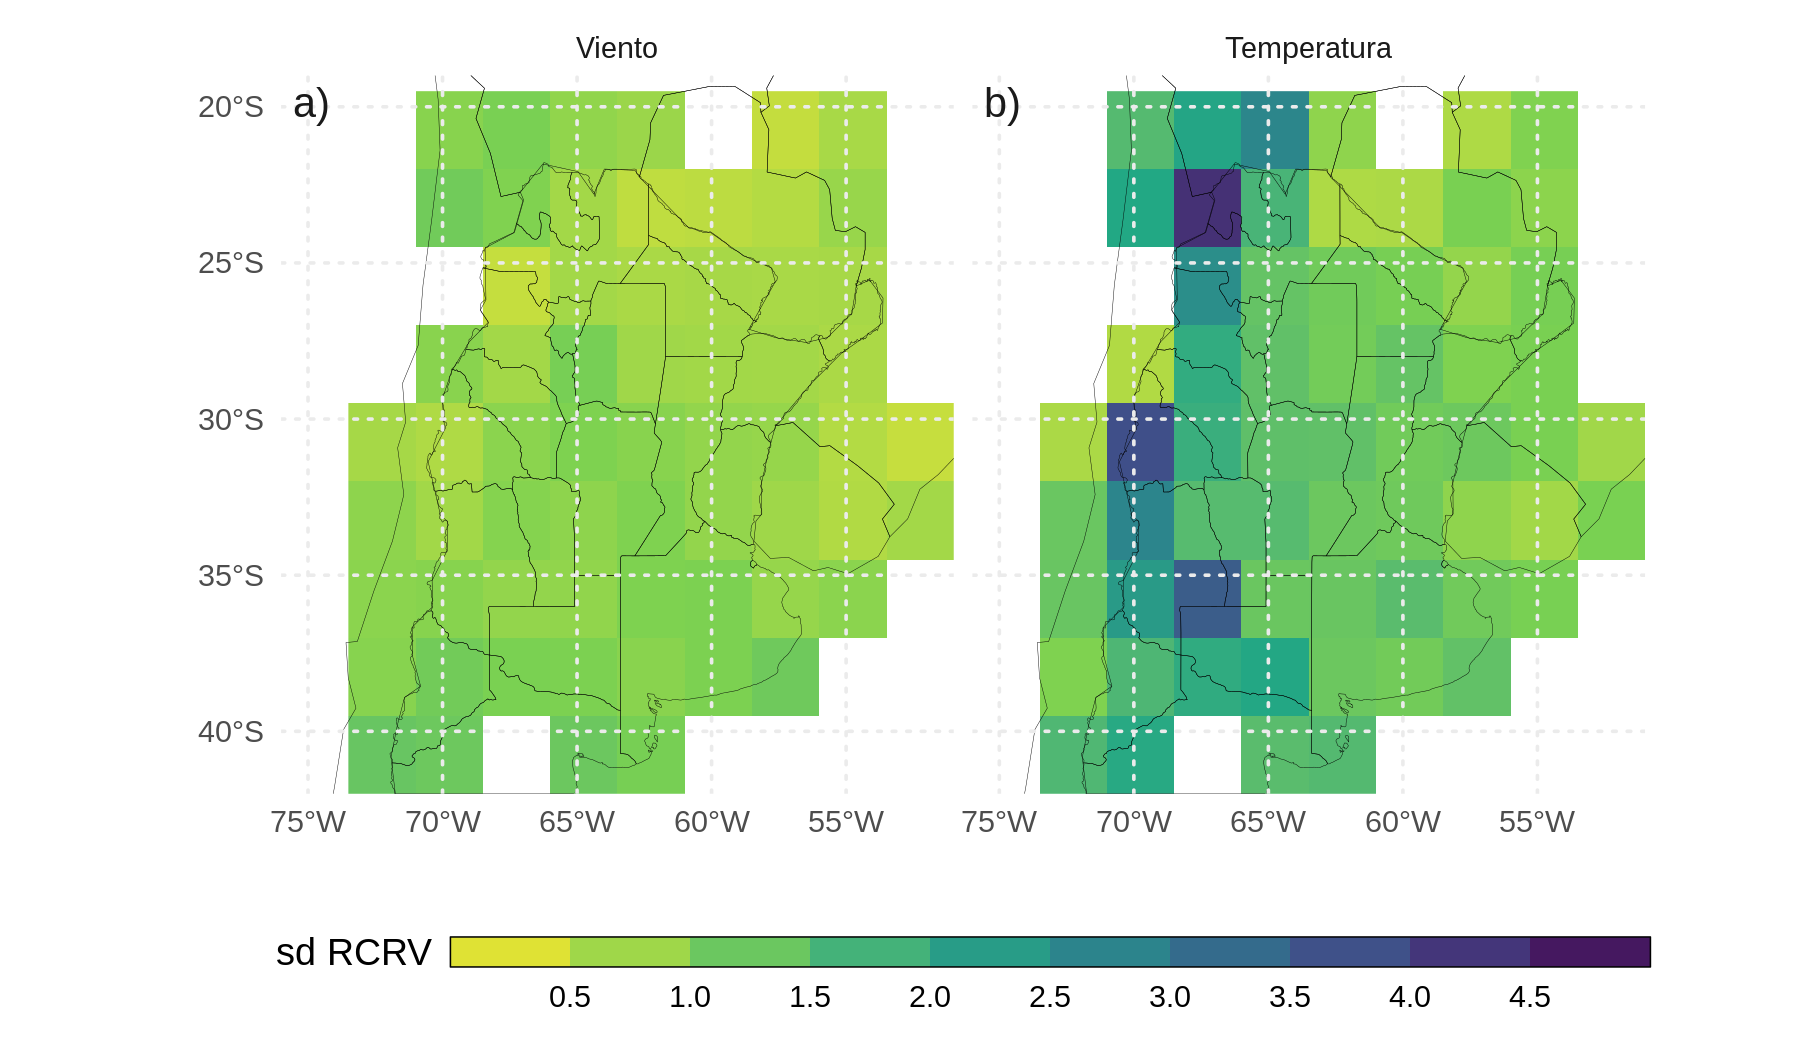
\includegraphics{thesis_files/figure-latex/rcrv-sfc-1} \caption{\(sd RCRV\) calculado para observaciones de superficie (de PREPBUFR y EMA) de a) viento, y b) temperatura promediados en cajas de 2.5º para el experimento RAD. Se usaron las observaciones agregadas de cada ciclo de asimilación horario paa todo el periodo del experimento.}\label{fig:rcrv-sfc}
\end{figure}

\begin{figure}
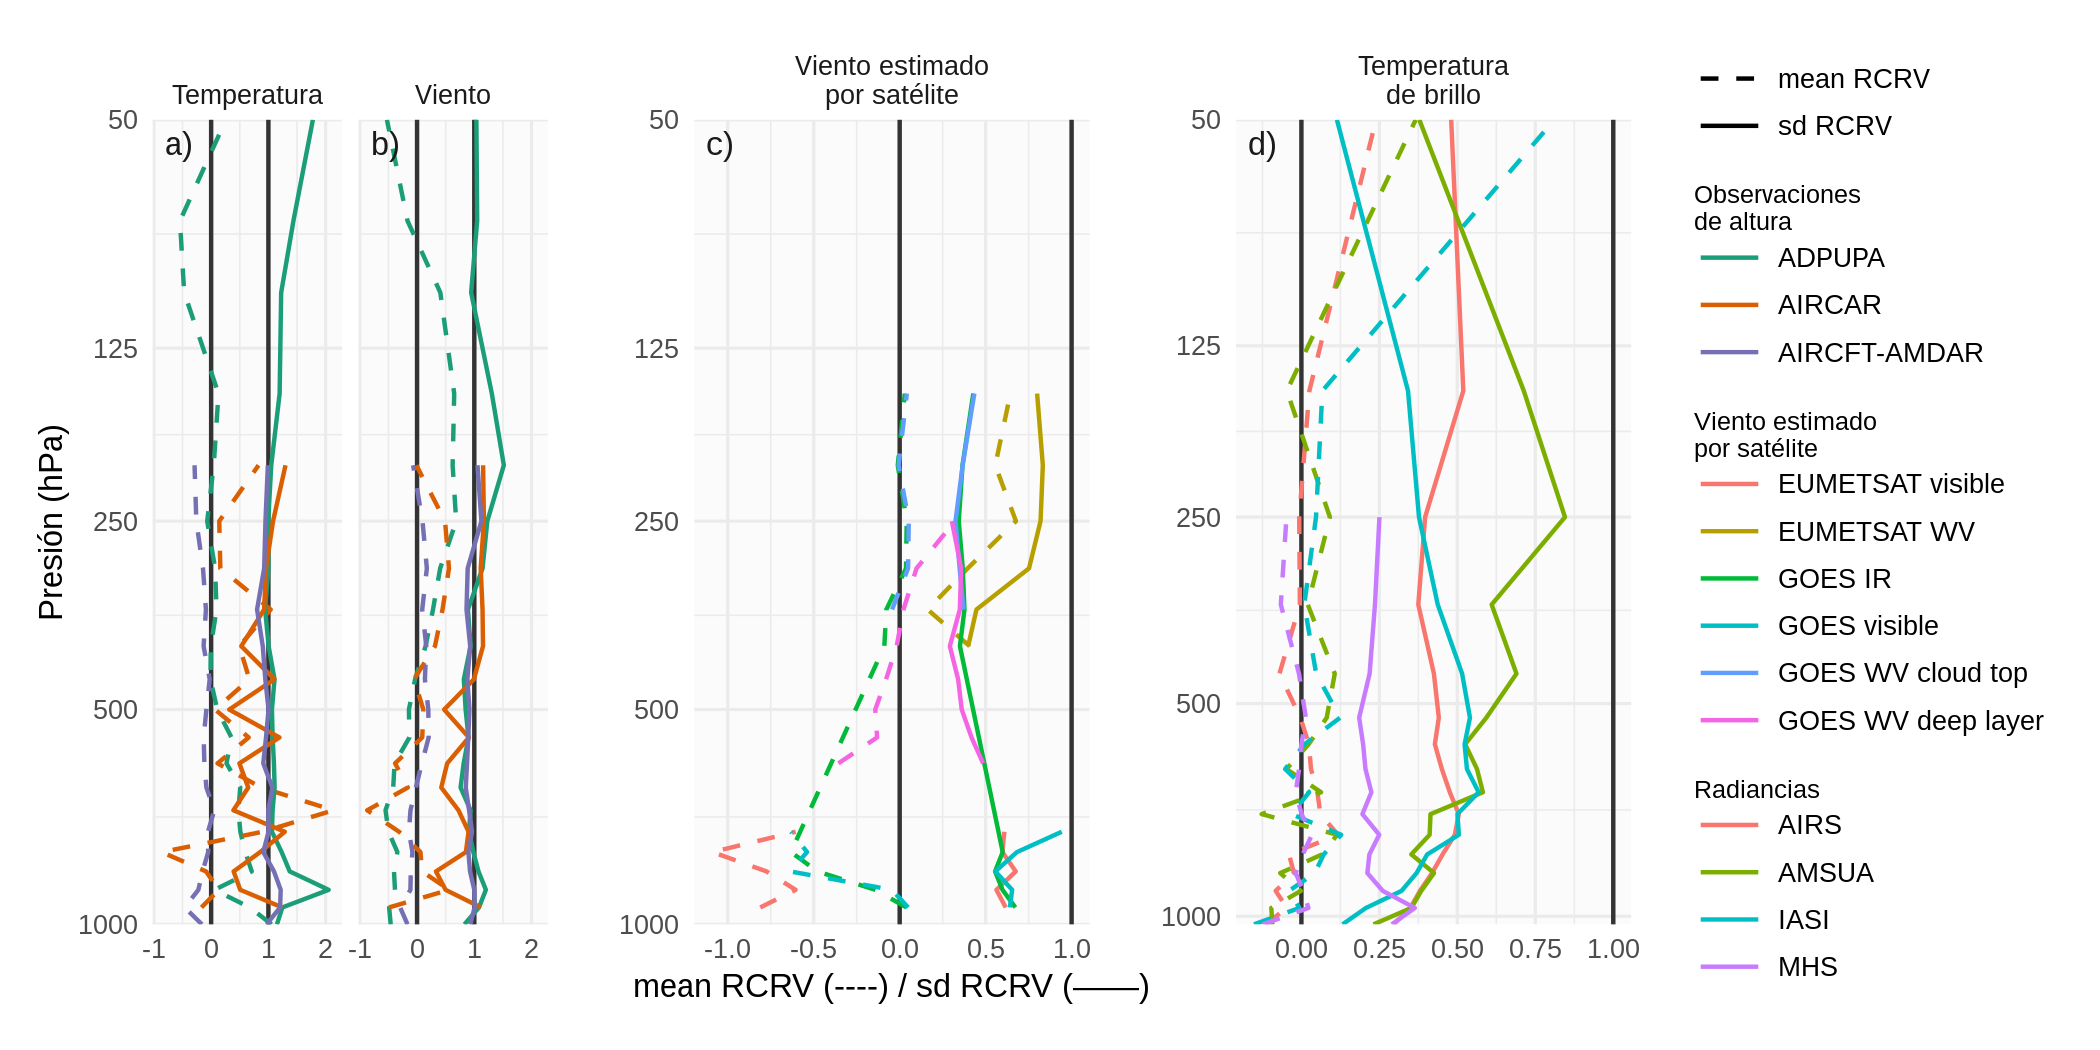
\includegraphics{thesis_files/figure-latex/rcrv-profile-1} \caption{Perfiles verticales de \(mean RCRV\) (línea punteada) y \(sd RCRV\) (línea sólida) para observaciones de a) temperatura y b) viento de sondeos y aviones, c) viento estimado por satélites, y d) temperatura de brillo para el experimento RAD. Se usaron las observaciones agregadas de cada ciclo de asimilación horario para todo el periodo del experimento.}\label{fig:rcrv-profile}
\end{figure}
\hypertarget{impacto-analisis}{%
\subsection{Impacto de la asimilación de las distintas observaciones}\label{impacto-analisis}}

Esta sección presenta el impacto de la asimilación de diferentes tipos de observación sobre algunas variables que son particularmente relevantes para el desarrollo de convección húmeda profunda. El análisis se realiza sobre un dominio más pequeño (recuadro rojo en la Figura \ref{fig:dominio}a) que corresponde a la región directamente afectada por el SCM. Las figuras \ref{fig:TQ-diff}a-c muestran la diferencia entre el perfil vertical de temperatura promediado espacialmente para el análisis de los experimentos. Al promediar las diferencias entre dos experimentos se puede aislar el impacto sistemático producido por los diferentes sistemas de observación sobre la situación analizada. Durante el primer día, la asimilación de las observaciones de EMA da como resultado el desarrollo de una PBL más fría. Este efecto de enfriamiento tiene un claro ciclo diurno, siendo más fuerte durante la noche (Figura \ref{fig:TQ-diff}a). Durante el segundo día del experimento, el impacto de las observaciones de EMA se extiende a la troposfera media y alta, coincidiendo con la fase madura del SCM. La diferencia positiva que se observa en AWS-CONV entre 500 y 200 hPa se produce por el desarrollo de convección más intensa en AWS en comparación con CONV. Este es un buen ejemplo de cómo la información en niveles bajos de la atmósfera proporcionada por las estaciones meteorológicas de superficie puede extenderse rápidamente a la troposfera en presencia de convección húmeda profunda. Aunque la circulación media y alta puede tener un impacto importante en la organización y evolución del SCM sobre la región, los vientos estimados por satélite no tuvieron un impacto apreciable en la temperatura y humedad media (Figura \ref{fig:TQ-diff}b-e), posiblemente debido a alto valor del error de estas observaciones utilizados para la asimilación.
Durante el primer día del experimento, la asimilación de las radiancias produce un efecto de calentamiento en la PBL que compensa parcialmente el efecto de enfriamiento de las observaciones de EMA (Figura \ref{fig:TQ-diff}c). No se encuentra un impacto sistemático claro por encima de la PBL durante este periodo para estas variables. Durante el segundo día, el impacto de las observaciones de radiancia se observa en toda la troposfera con una distribución que es similar al impacto encontrado en el experimento AWS pero con signo opuesto.

Comparando la representación de la humedad específica en los experimentos (Figuras \ref{fig:TQ-diff}d-f), el impacto de la asimilación de EMA, que tienen una resolución espacial y temporal mayor, es muy importante en niveles bajos (Figura \ref{fig:TQ-diff}d). La PBL en el experimento AWS es sistemáticamente más húmeda que en el experimento CONV, especialmente durante la noche. El aumento de la humedad en niveles bajos gracias a la asimilación de observaciones de una red de superficie más densa corrige el bias seco reportado previamente en el modelo WRF sobre la región (Ruiz et al., 2010; Matsudo et al., 2021; Casaretto et al., 2022). El humedecimiento de la PBL es impulsado principalmente por la covarianza entre la temperatura y la humedad específica dentro de la PBL. En el experimento y sobre el centro del dominio, esta covarianza se mantiene negativa, generando un aumento de la humedad en niveles bajos a medida que las observaciones introducen correcciones negativas de temperatura. Como en el caso de la temperatura, el impacto sistemático de los vientos estimados por satélite sobre la humedad es pequeño (Figura \ref{fig:TQ-diff}e). La figura \ref{fig:TQ-diff}f muestra que las radiancias reducen la humedad en niveles medios y bajos durante el primer día del experimento. El efecto de secamiento se extiende a niveles medios y bajos durante el segundo día del experimento, coincidiendo con el desarrollo del SCM entre las 00 y las 12 UTC del 22 de noviembre.


\begin{figure}

{\centering 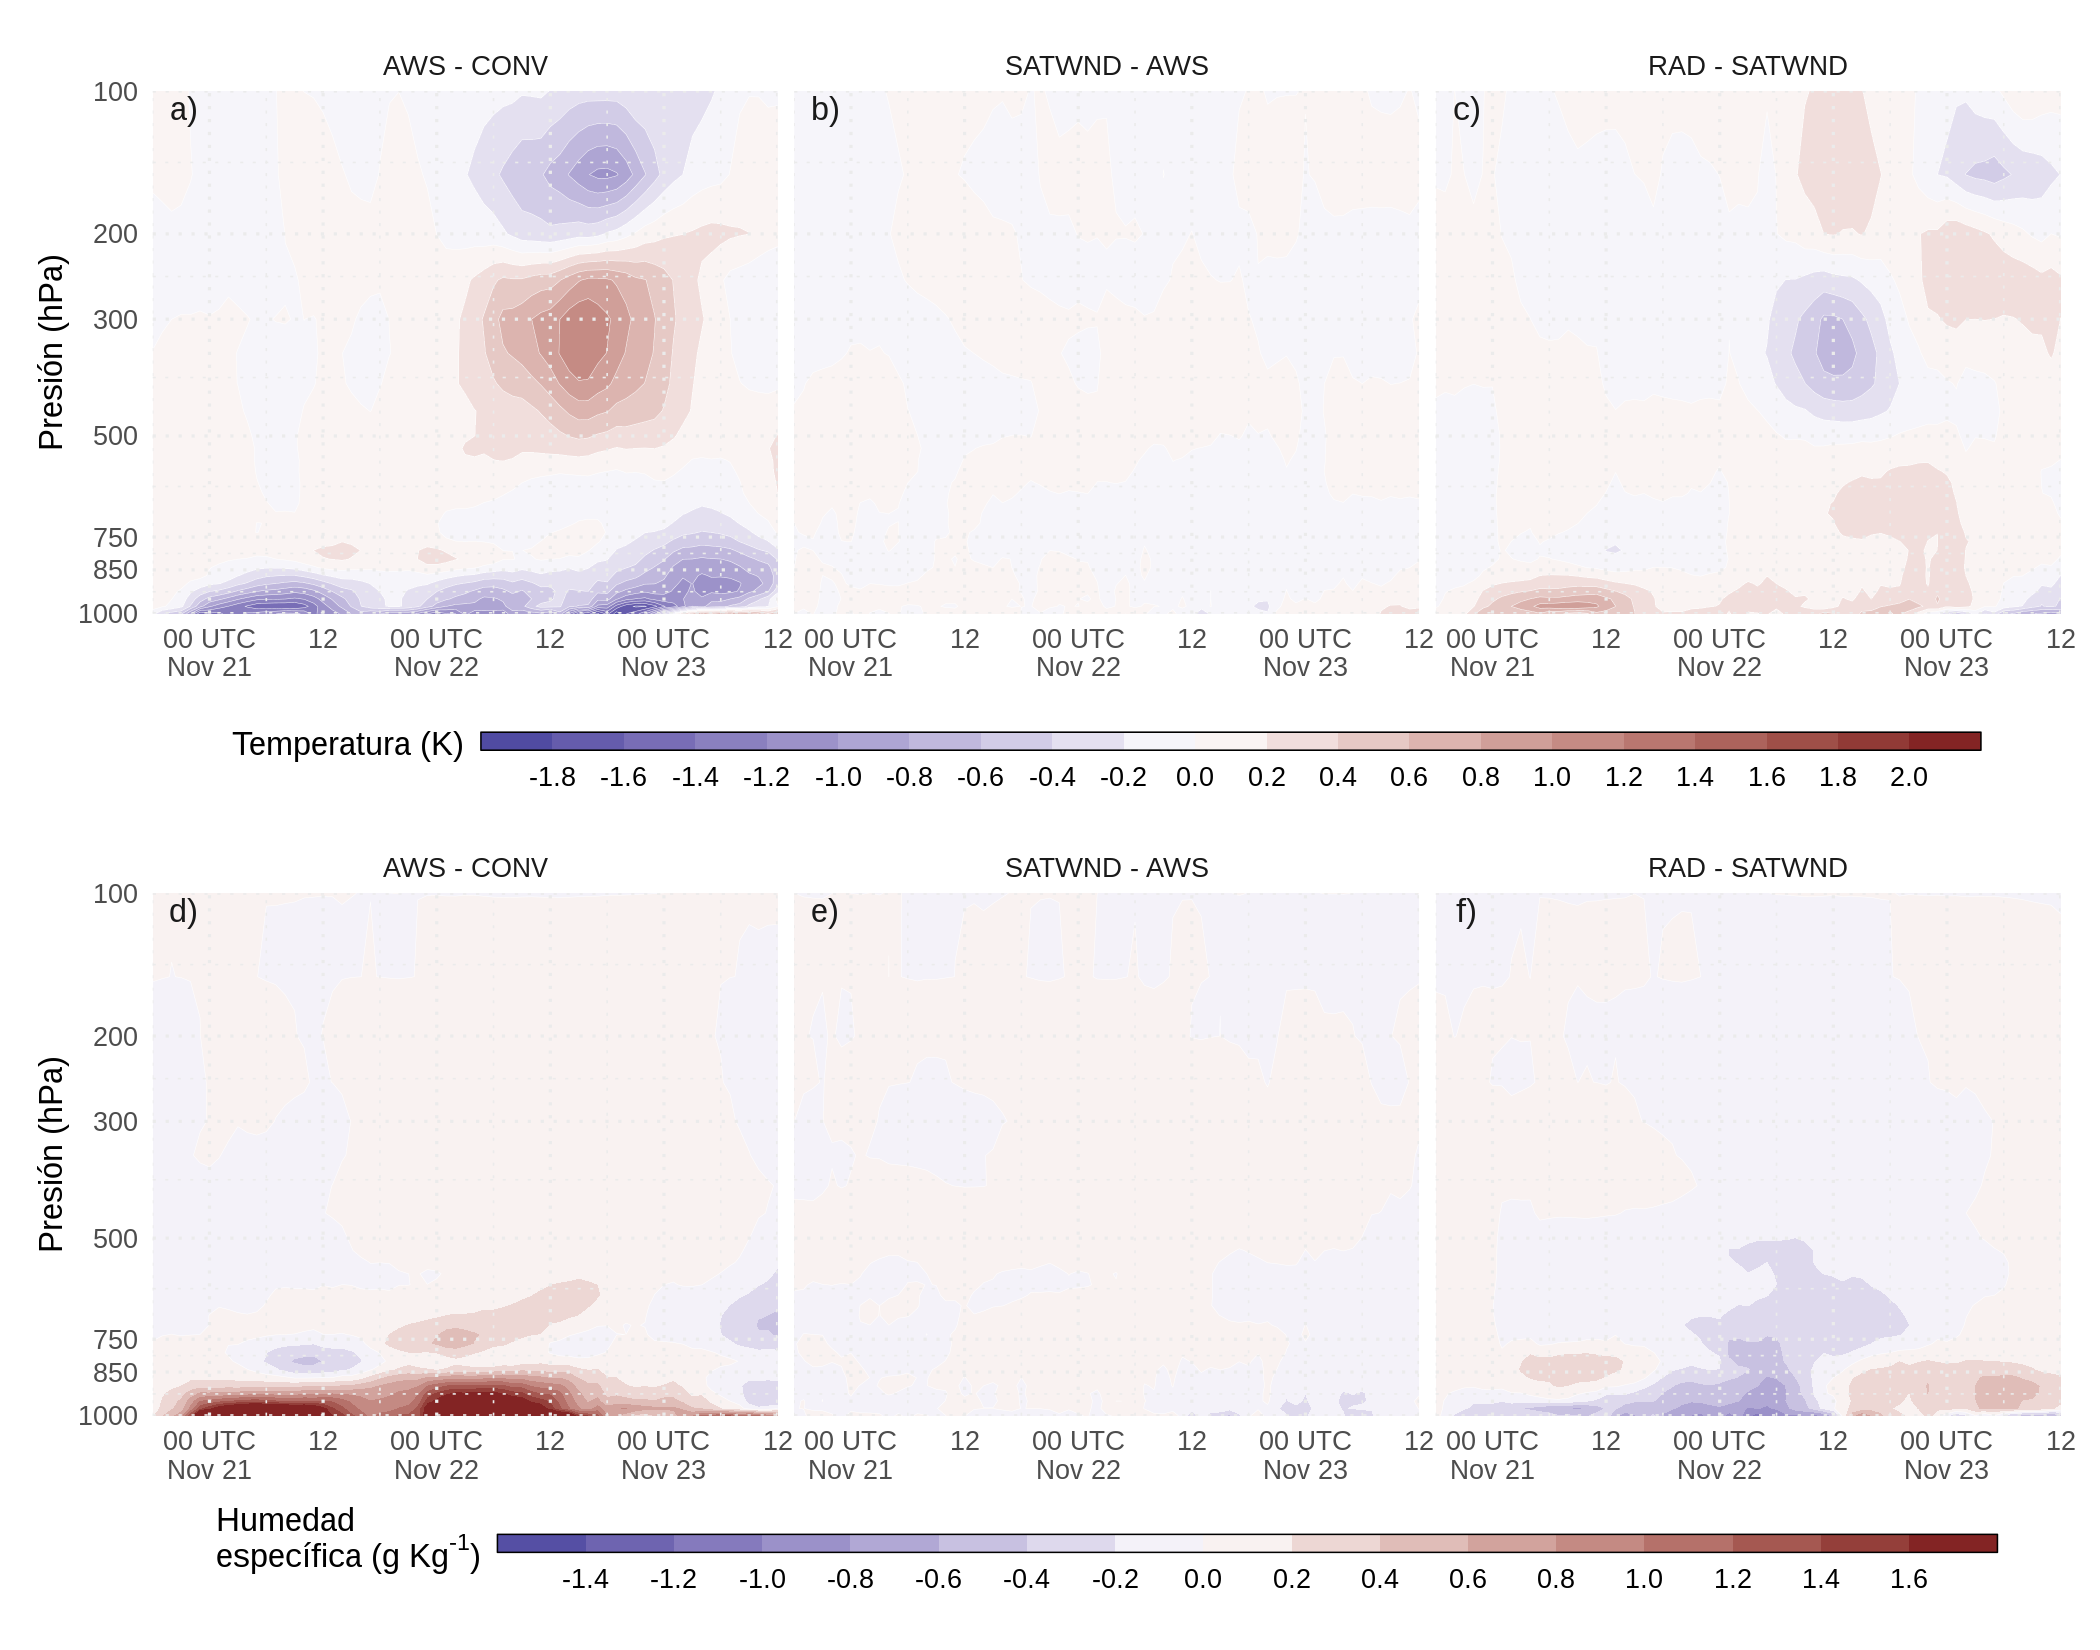
\includegraphics{thesis_files/figure-latex/TQ-diff-1} 

}

\caption{Diferencia entre la media del ensamble de los análisis a) y d) AWS-CONV, b) y e) SATWND-AWS, y c) y f) RAD-SATWND para los perfiles verticales espacialmente promediados de la temperatura (a, b y c, en \(K\)) y la humedad específica (d, e y f en \(g\ kg^{-1}\)) calculados sobre el dominio interior (recuadro rojo en la Figura \ref{fig:dominio}a) para cada ciclo de análisis.}\label{fig:TQ-diff}
\end{figure}
El impacto que genera la asimilación de las observaciones de EMA se puede observar con mayor detalle en las Figuras \ref{fig:ana-guess} donde se muestran perfiles verticales medios a lo largo del tiempo para la diferencia entre el análisis y el campo preliminar o \emph{actualización}. Las observaciones convencionales y en particular los sondeos operativos generan un calentamiento de la PBL en CONV, particularmente previo al derarrollo de la convección (Figura \ref{fig:ana-guess}a). Por otro lado las observaciones de EMA disminuyen la temperatura en niveles bajos durante la noche y la aumentan durante el día, lo que podría indicar que el modelo genera una PBL con menos variabilidad de temperatura. Luego del desarrollo de la convección, el impacto de las observaciones de EMA está asociado a un enfriamiento de la capa límite que podrían estar corrigiendo un frente frío débil generado por el modelo (Figura \ref{fig:ana-guess}b). En las Figuras \ref{fig:ana-guess}c-d se observa nuevamente un aumento de la humedad en niveles bajos gracias a la asimilación de observaciones de EMA particularmente durante la noche disminuyendo el bias seco presente en el modelo.


\begin{figure}

{\centering 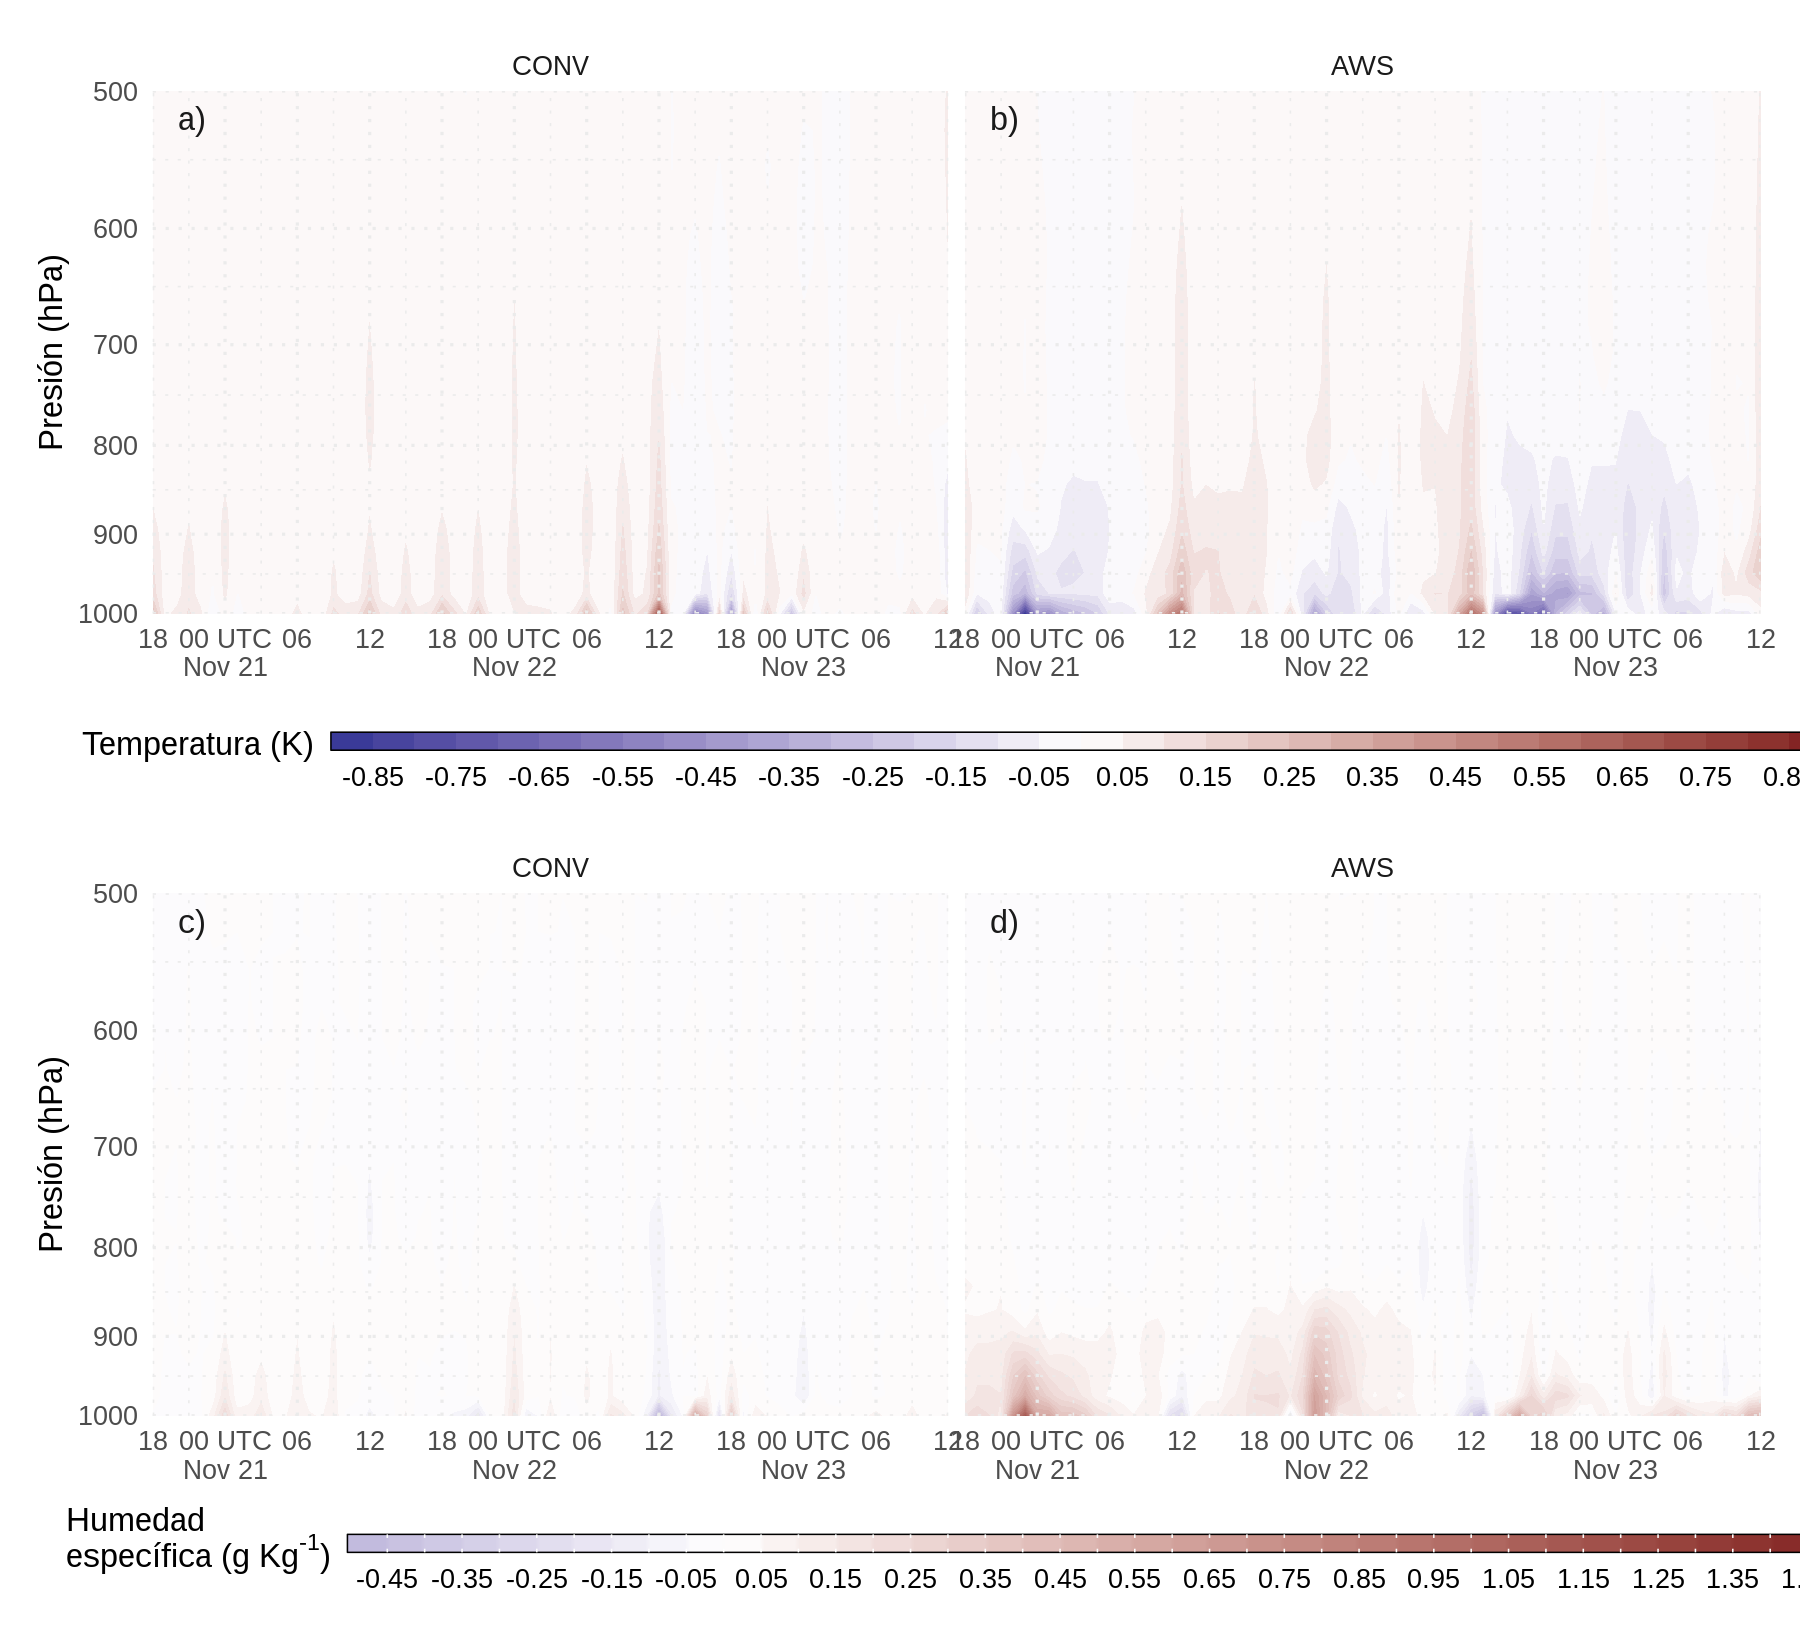
\includegraphics{thesis_files/figure-latex/ana-guess-1} 

}

\caption{Perfiles verticales medios de la diferencia entre el análisis y el campo preliminar para a) y d) CONV, b) y b) y d) AWS para los perfiles verticales espacialmente promediados de la temperatura (a y b en \(K\)) y la humedad específica (d y c en \(g\ kg^{-1}\)) calculados sobre el dominio interior (recuadro rojo en la Figura \ref{fig:dominio}a) para cada ciclo de análisis.}\label{fig:ana-guess}
\end{figure}
El impacto en las componentes del viento se muestran en la Figura \ref{fig:UV-diff}, junto con la correspondiente componente del viento promediada en el experimento con el mayor número de observaciones asimiladas (por ejemplo, la Figura \ref{fig:UV-diff}a muestra la diferencia de viento zonal entre AWS y CONV y el viento zonal para AWS). La asimilación de EMA produce un viento más del este y menos del norte en niveles bajos durante los dos primeros días de análisis (Figuras \ref{fig:UV-diff}a,b). Existe un ciclo diurno asociado al impacto de las estaciones meteorológicas automáticas sobre el viento meridional (Figura \ref{fig:UV-diff}d) con una mayor reducción del viento del norte durante las horas nocturnas. Esto indica que las observaciones en superficie están reduciendo la intensidad del jet de capas bajas presente en el entorno preconvectivo. Después de las 18 UTC del 22 de noviembre, se observa el efecto contrario cuando el SCM se desplaza por el dominio hacia el noreste. Tras el inicio de las celdas convectivas, el impacto sistemático en el campo de viento es mayor en los niveles medios y altos (Figuras \ref{fig:UV-diff}d, f). Durante los días 22 y 23 de noviembre el impacto de asimilar EMA produce un aumento del viento del norte en los niveles superiores de la tropósfera. Esto podría ser una consecuencia de un SCM más intenso que produce un aumento del flujo de salida del lado polar de la tormenta. Aunque las observaciones de viento estimada por satélites producen el mayor impacto en niveles medios y altos, donde el número de observaciones es mayor, el impacto sistemático es en general menor que el producido por la asimilación de datos de EMA (Figuras \ref{fig:UV-diff}b, e). La razón del pequeño impacto observado en SATWND podría estar asociada al valor del error de observación utilizado para la asimilación de estas observaciones.

La asimilación de las radiancias produce una reducción del viento del oeste con respecto a SATWND en niveles bajos y altos (Figura \ref{fig:UV-diff}c). Para el viento meridional, estas observaciones producen un aumento 1 \(ms^{-1}\) en el flujo del norte en niveles bajos, opuesto al generado por la asimilación de las observaciones de EMA durante la noche, entre las 03 y las 12 UTC, previas al desarrollo del SCM (Figura \ref{fig:UV-diff}f). En niveles superiores y durante los días 22 y 23 de noviembre, el impacto medio de la asimilación de radiancias es una disminución de la velocidad del viento. El campo de viento meridional a 200 hPa en diferentes momentos muestra que el flujo de salida del SCM es aún más intenso que en los otros experimentos, mientras que el viento sur por delante del SCM también aumenta produciendo una reducción media del viento del norte (Figura \ref{fig:UV-diff}f).


\begin{figure}

{\centering 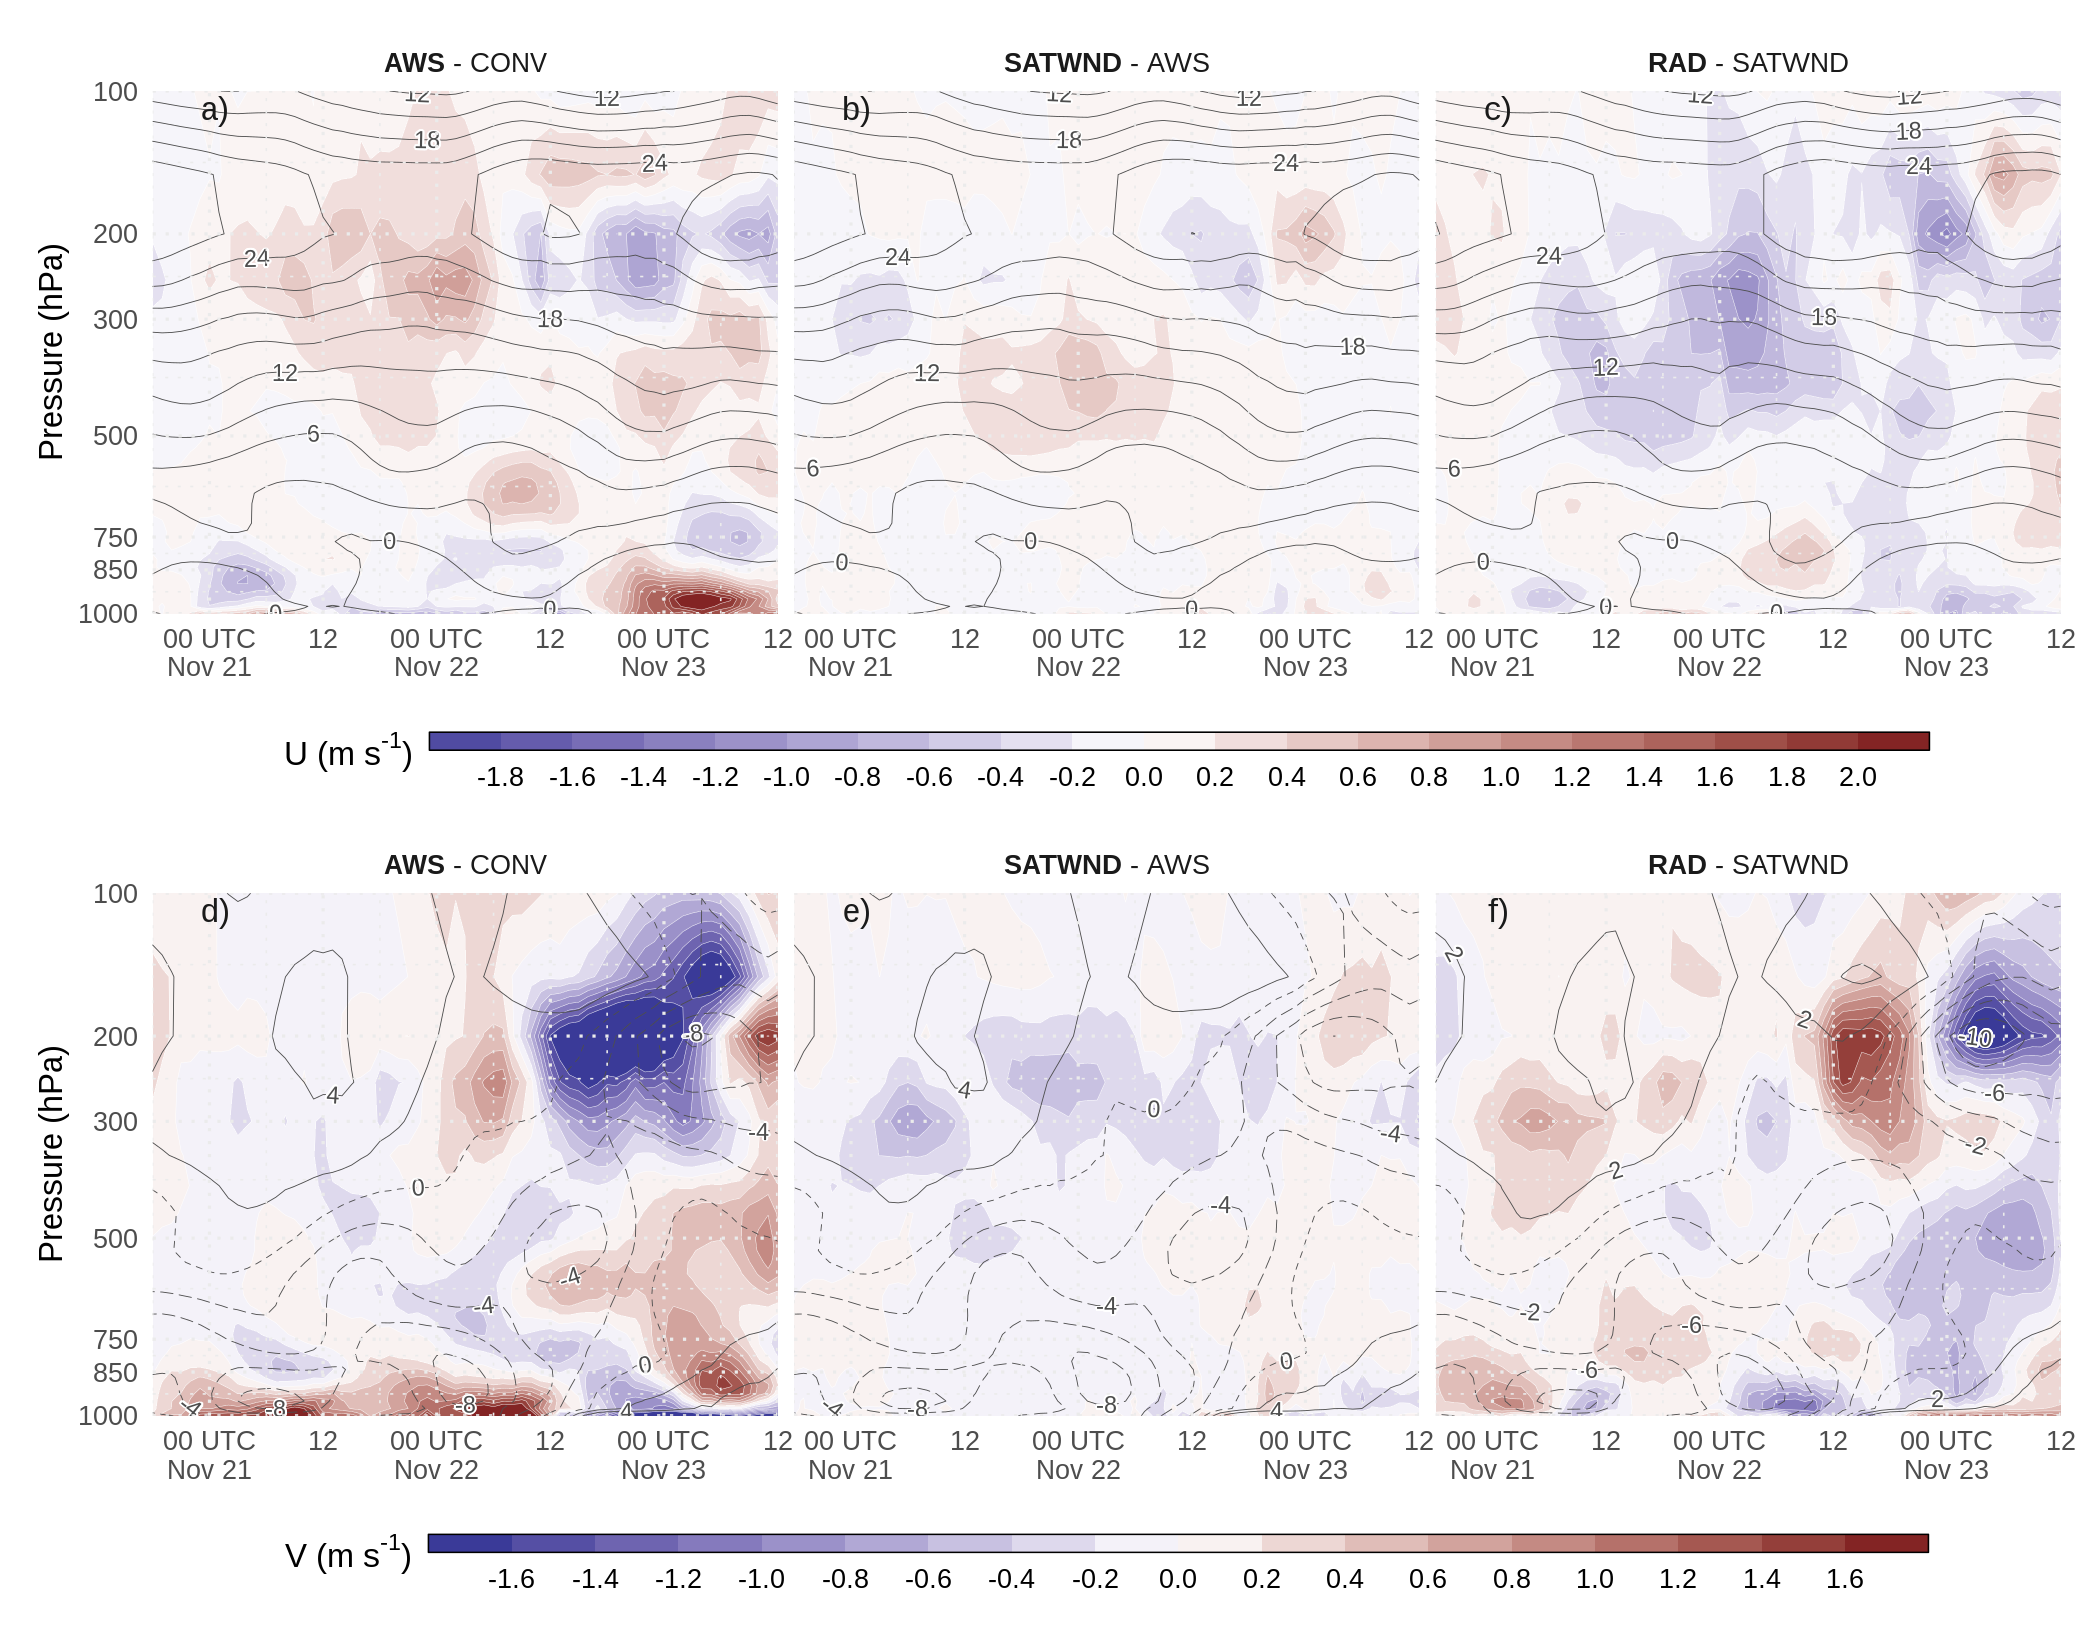
\includegraphics{thesis_files/figure-latex/UV-diff-1} 

}

\caption{Diferencia entre la media del ensamble de los análisis a) y d) AWS-CONV, b) y e) SATWND-AWS, y c) y f) RAD-SATWND para los perfiles verticales espacialmente promediados del viento zonal (a, b y c, en \(K\)) y viento meridional (d, e y f en \(g\ kg^{-1}\)) calculados sobre el dominio interior (recuadro rojo en la Figura \ref{fig:dominio}a) para cada ciclo de análisis. Los contornos negros corresponden al viento zonal y meridional para (a,d) AWS, (b,e) SATWND, y (c,f) RAD ya que son los experimentos tienen más observaciones asimiladas en cada panel.}\label{fig:UV-diff}
\end{figure}
La diferencia entre ERA5 (Hersbach et al., 2018) y la media del ensamble del análisis para cada experimento se compara en la Figura \ref{fig:era5}, apoyando los resultados observados en las Figuras \ref{fig:TQ-diff} y \ref{fig:UV-diff}. En concreto, la Figura \ref{fig:era5}a muestra un bias cálido en los niveles bajos (es decir, CONV es más cálido que ERA5) que disminuye en la Figura \ref{fig:era5}b cuando se asimilan las observaciones de EMA. En la misma dirección, la Figura \ref{fig:TQ-diff}a muestra una diferencia negativa entre AWS y CONV, lo que significa que las observaciones de EMA están enfriando los niveles bajos de la atmósfera. Comparando ERA5-RAD (Figura \ref{fig:era5}d), hay un pequeño aumento del bias cálido, asociado al calentamiento producido por la asimilación de las observaciones de radiancia, como se muestra en la Figura \ref{fig:TQ-diff}c.~Un efecto similar puede observarse en la humedad específica, las observaciones de EMA corrigen parcialmente el bias seco presente en la Figura \ref{fig:era5}e y la asimilación de las observaciones de radiancia reduce el impacto positivo de EMA. El impacto sobre las componentes del viento es menor, por lo que sólo se incluye el viento meridional en las figuras \ref{fig:era5}i-l, que muestran que las observaciones de radiancia son las principales responsables del impacto positivo observado en el análisis al reducir la distancia ERA5-RAD, en particular durante la fase madura del MCS. En general, los ajustes asociados a la asimilación de las observaciones de radiancia y de EMA conducen a un análisis más cercano a los reanálisis ERA5.


\begin{figure}

{\centering 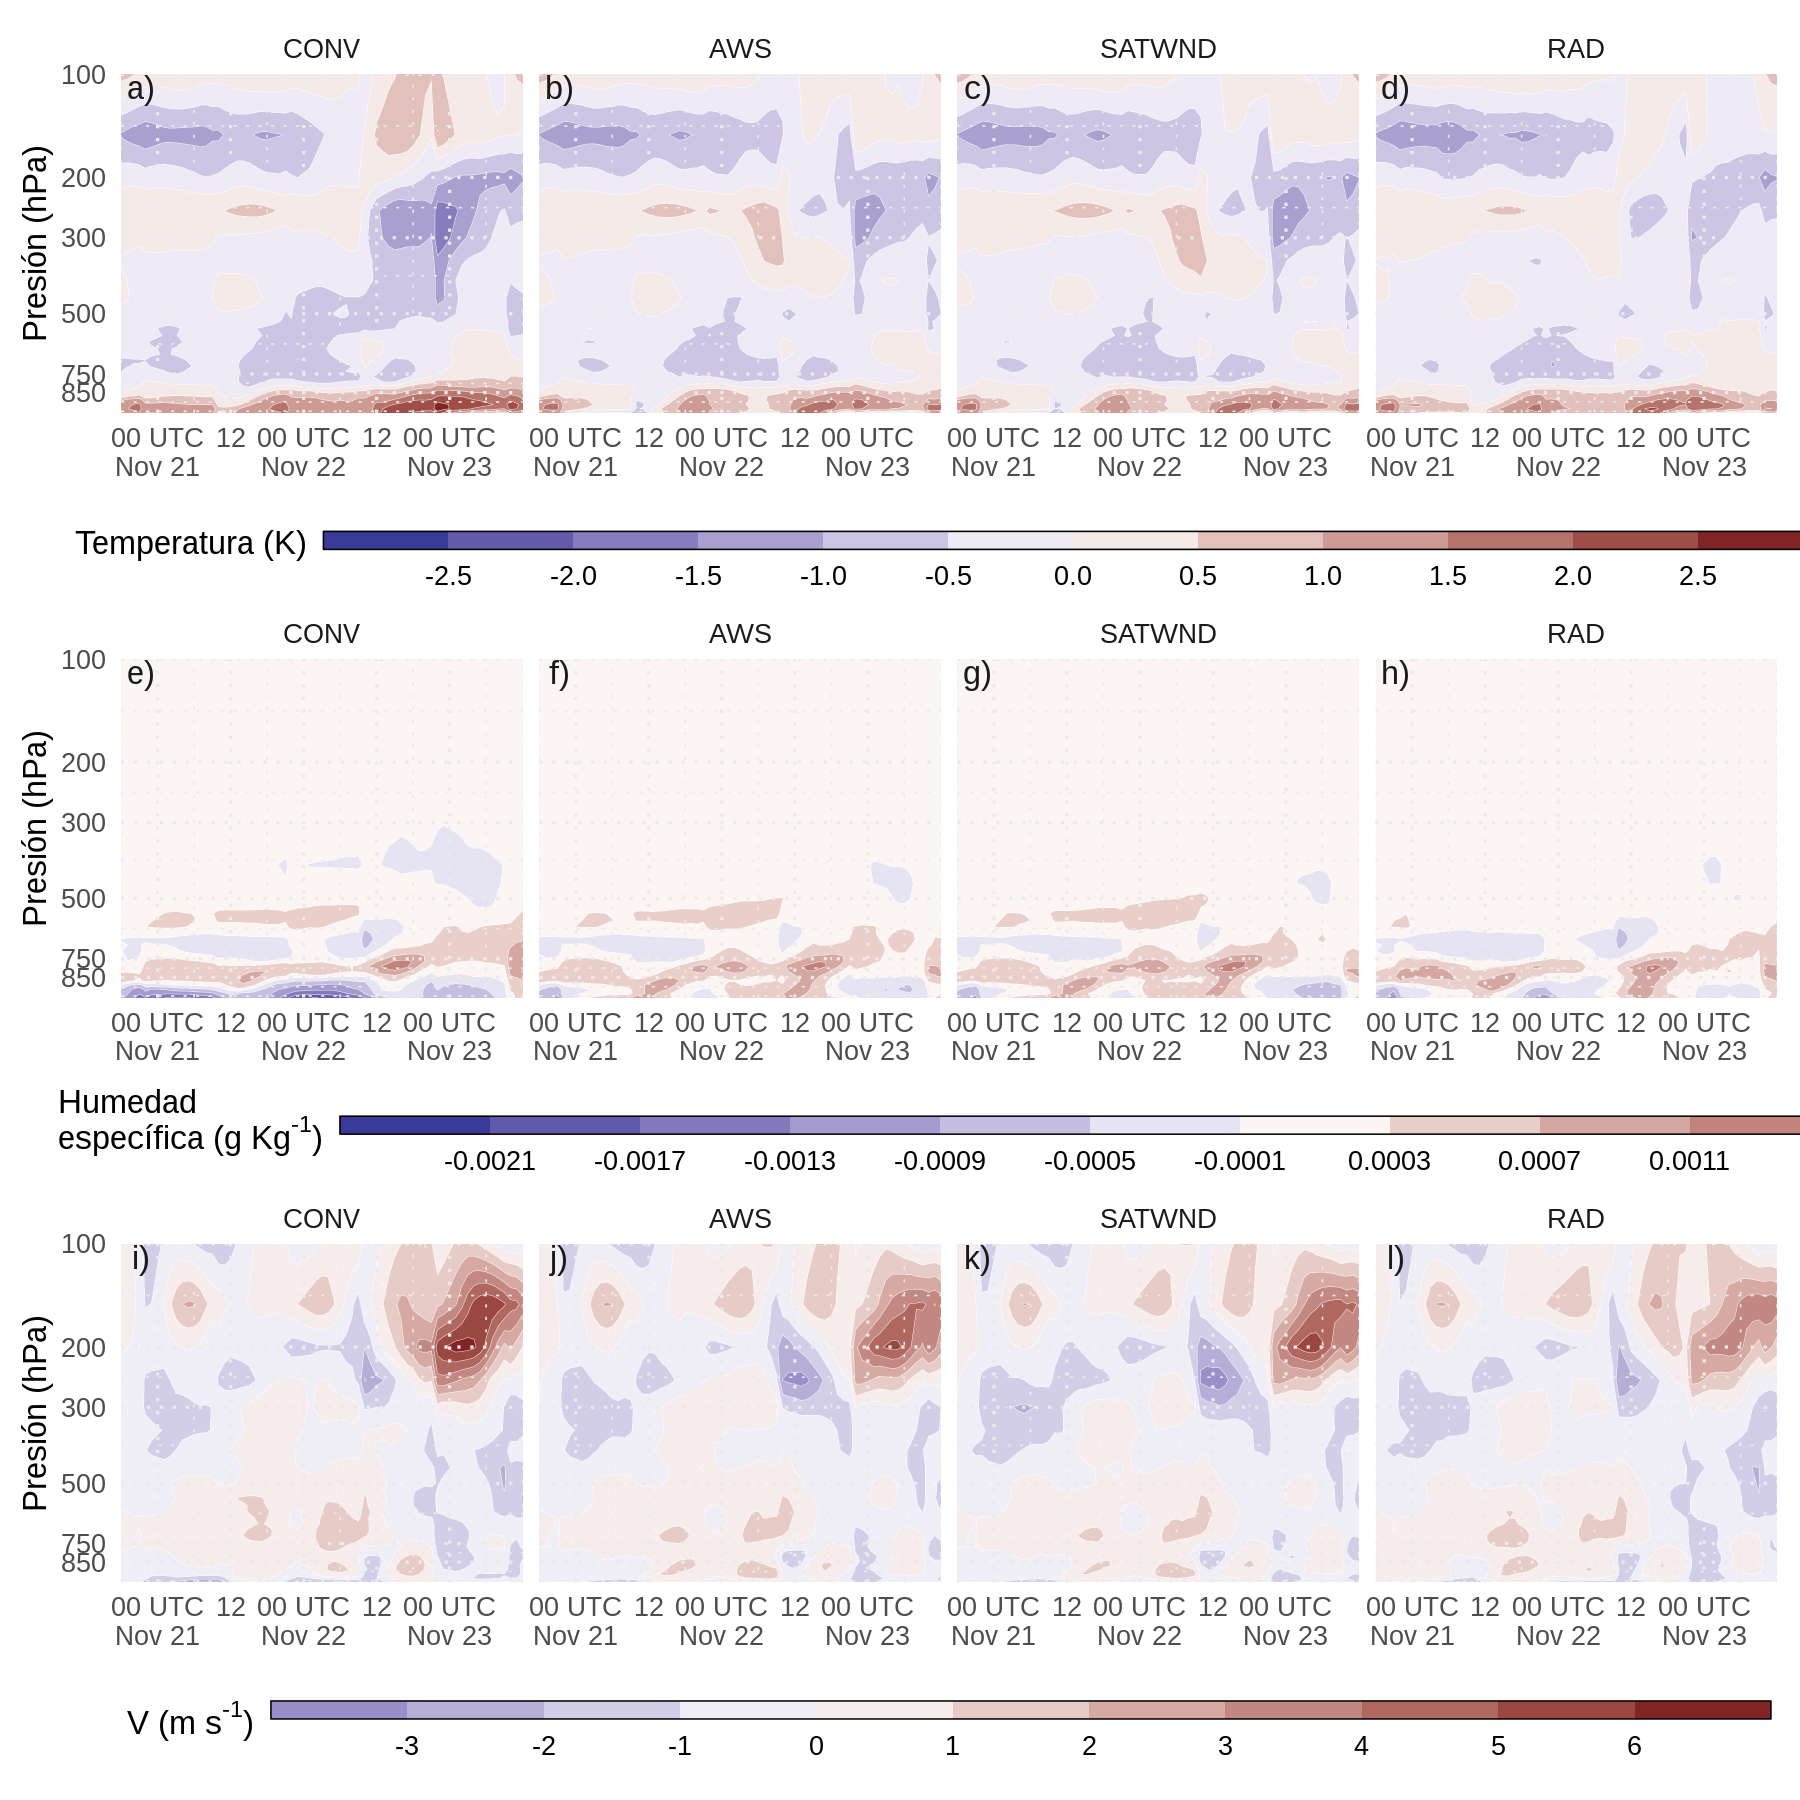
\includegraphics{thesis_files/figure-latex/era5-1} 

}

\caption{Diferencia entre la media del ensamble del análisis de cada experimento y el ERA5 para los perfiles verticales espacialmente promediados de la temperatura del aire (K, a--d), la humedad específica (\(g\ Kg^{-1}\), e--h) y el viento meridional (\(m\ s^{-1}\), i--l) calculados sobre el dominio interior (recuadro rojo en la Figura \ref{fig:dominio}a) para cada ciclo de análisis.}\label{fig:era5}
\end{figure}
Para investigar cómo los cambios en la PBL pueden modificar el entorno preconvectivo, se compara la distribución horizontal media de análisis del viento meridional del norte (para los primeros 7 niveles sigma), el agua precipitable, la temperatura en niveles bajos y el CAPE. A las 00 UTC del 22 de noviembre (después de 30 ciclos de asimilación) las primeras células convectivas se estaban desarrollando sobre la región sur del dominio a lo largo del frente frío. La figura \ref{fig:summary-fields}a muestra el agua precipitable (sombreada) y la componente de viento meridional en niveles bajos promediada verticalmente (contornos). La figura muestra que la región húmeda que se extiende en la zona norte del dominio se ve reforzada por la asimilación de las observaciones de superficie de EMA. El aumento de la humedad es particularmente intenso en el extremo sur de esta región, justo por delante del frente frío donde se produce la iniciación de la convección. Los experimentos AWS y SATWND son muy similares, con valores de agua precipitable superiores a 55 \(kgm^{-2}\) al norte de 30\(^{\circ}\)S y una distribución vertical similar de la humedad específica (no mostrada). RAD tiene un contenido de agua precipitable menor que AWS y SATWND, pero mayor que CONV. La distribución de la humedad en niveles bajos en RAD parece ser el resultado de la combinación del efecto de humedecimiento de la asimilación de EMA -compensado parcialmente por la asimilación de las observaciones de radiancia- y un menor transporte meridional de humedad debido al flujo más débil del norte sobre el centro del dominio en comparación con CONV.

La distribución de la temperatura y la humedad en la PBL (Figura \ref{fig:summary-fields}b) se asemeja a las características observadas en los perfiles de temperatura (Figura \ref{fig:TQ-diff}a-c) donde AWS produce una PBL más fría que CONV mientras que la PBL en RAD es más cálida que en SATWND. En promedio, la PBL en AWS y SATWND es más fría que en CONV, mientras que RAD muestra una PBL más cálida que AWS debido a la asimilación de radiacias. Una PBL más cálida aumenta la inestabilidad potencial y ayuda a generar un entorno adecuado para el desarrollo de la convección profunda. La figura \ref{fig:summary-fields}c muestra la energía potencial convectiva disponible para el nivel (o parcela) más inestable (MCAPE, sombreada) y la cortante del viento entre 0 a 6 \(km\). Los valores de MCAPE en CONV no superan los 2000 \(J\ Kg^{-1}\) mientras que en el resto de los experimentos el MCAPE máximo supera los 4000 \(J\ Kg^{-1}\). El MCAPE en el experimento RAD es menor en comparación con AWS o SATWND. Esto es consistente con una menor humedad en la PBL con respecto a estos experimentos pero puede ser parcialmente compensado por una PBL ligeramente más cálida en el experimento RAD. La cortante del viento es más intensa en AWS, SATWND y RAD, alcanzando valores superiores a 15 \(m\ s^{-1}\) en el extremo sur de la región con valores positivos de MCAPE. Además, en esta misma región, estos experimentos muestran valores de MCAPE mayores que CONV. Cortantes de viento superior a 15 \(m\ s^{-1}\) están asociadas al desarrollo de SCMs más intensos y organizados (Chen et al., 2015) y también a condiciones favorables para el desarrollo de superceldas (Markowski and Richardson, 2010).


\begin{figure}
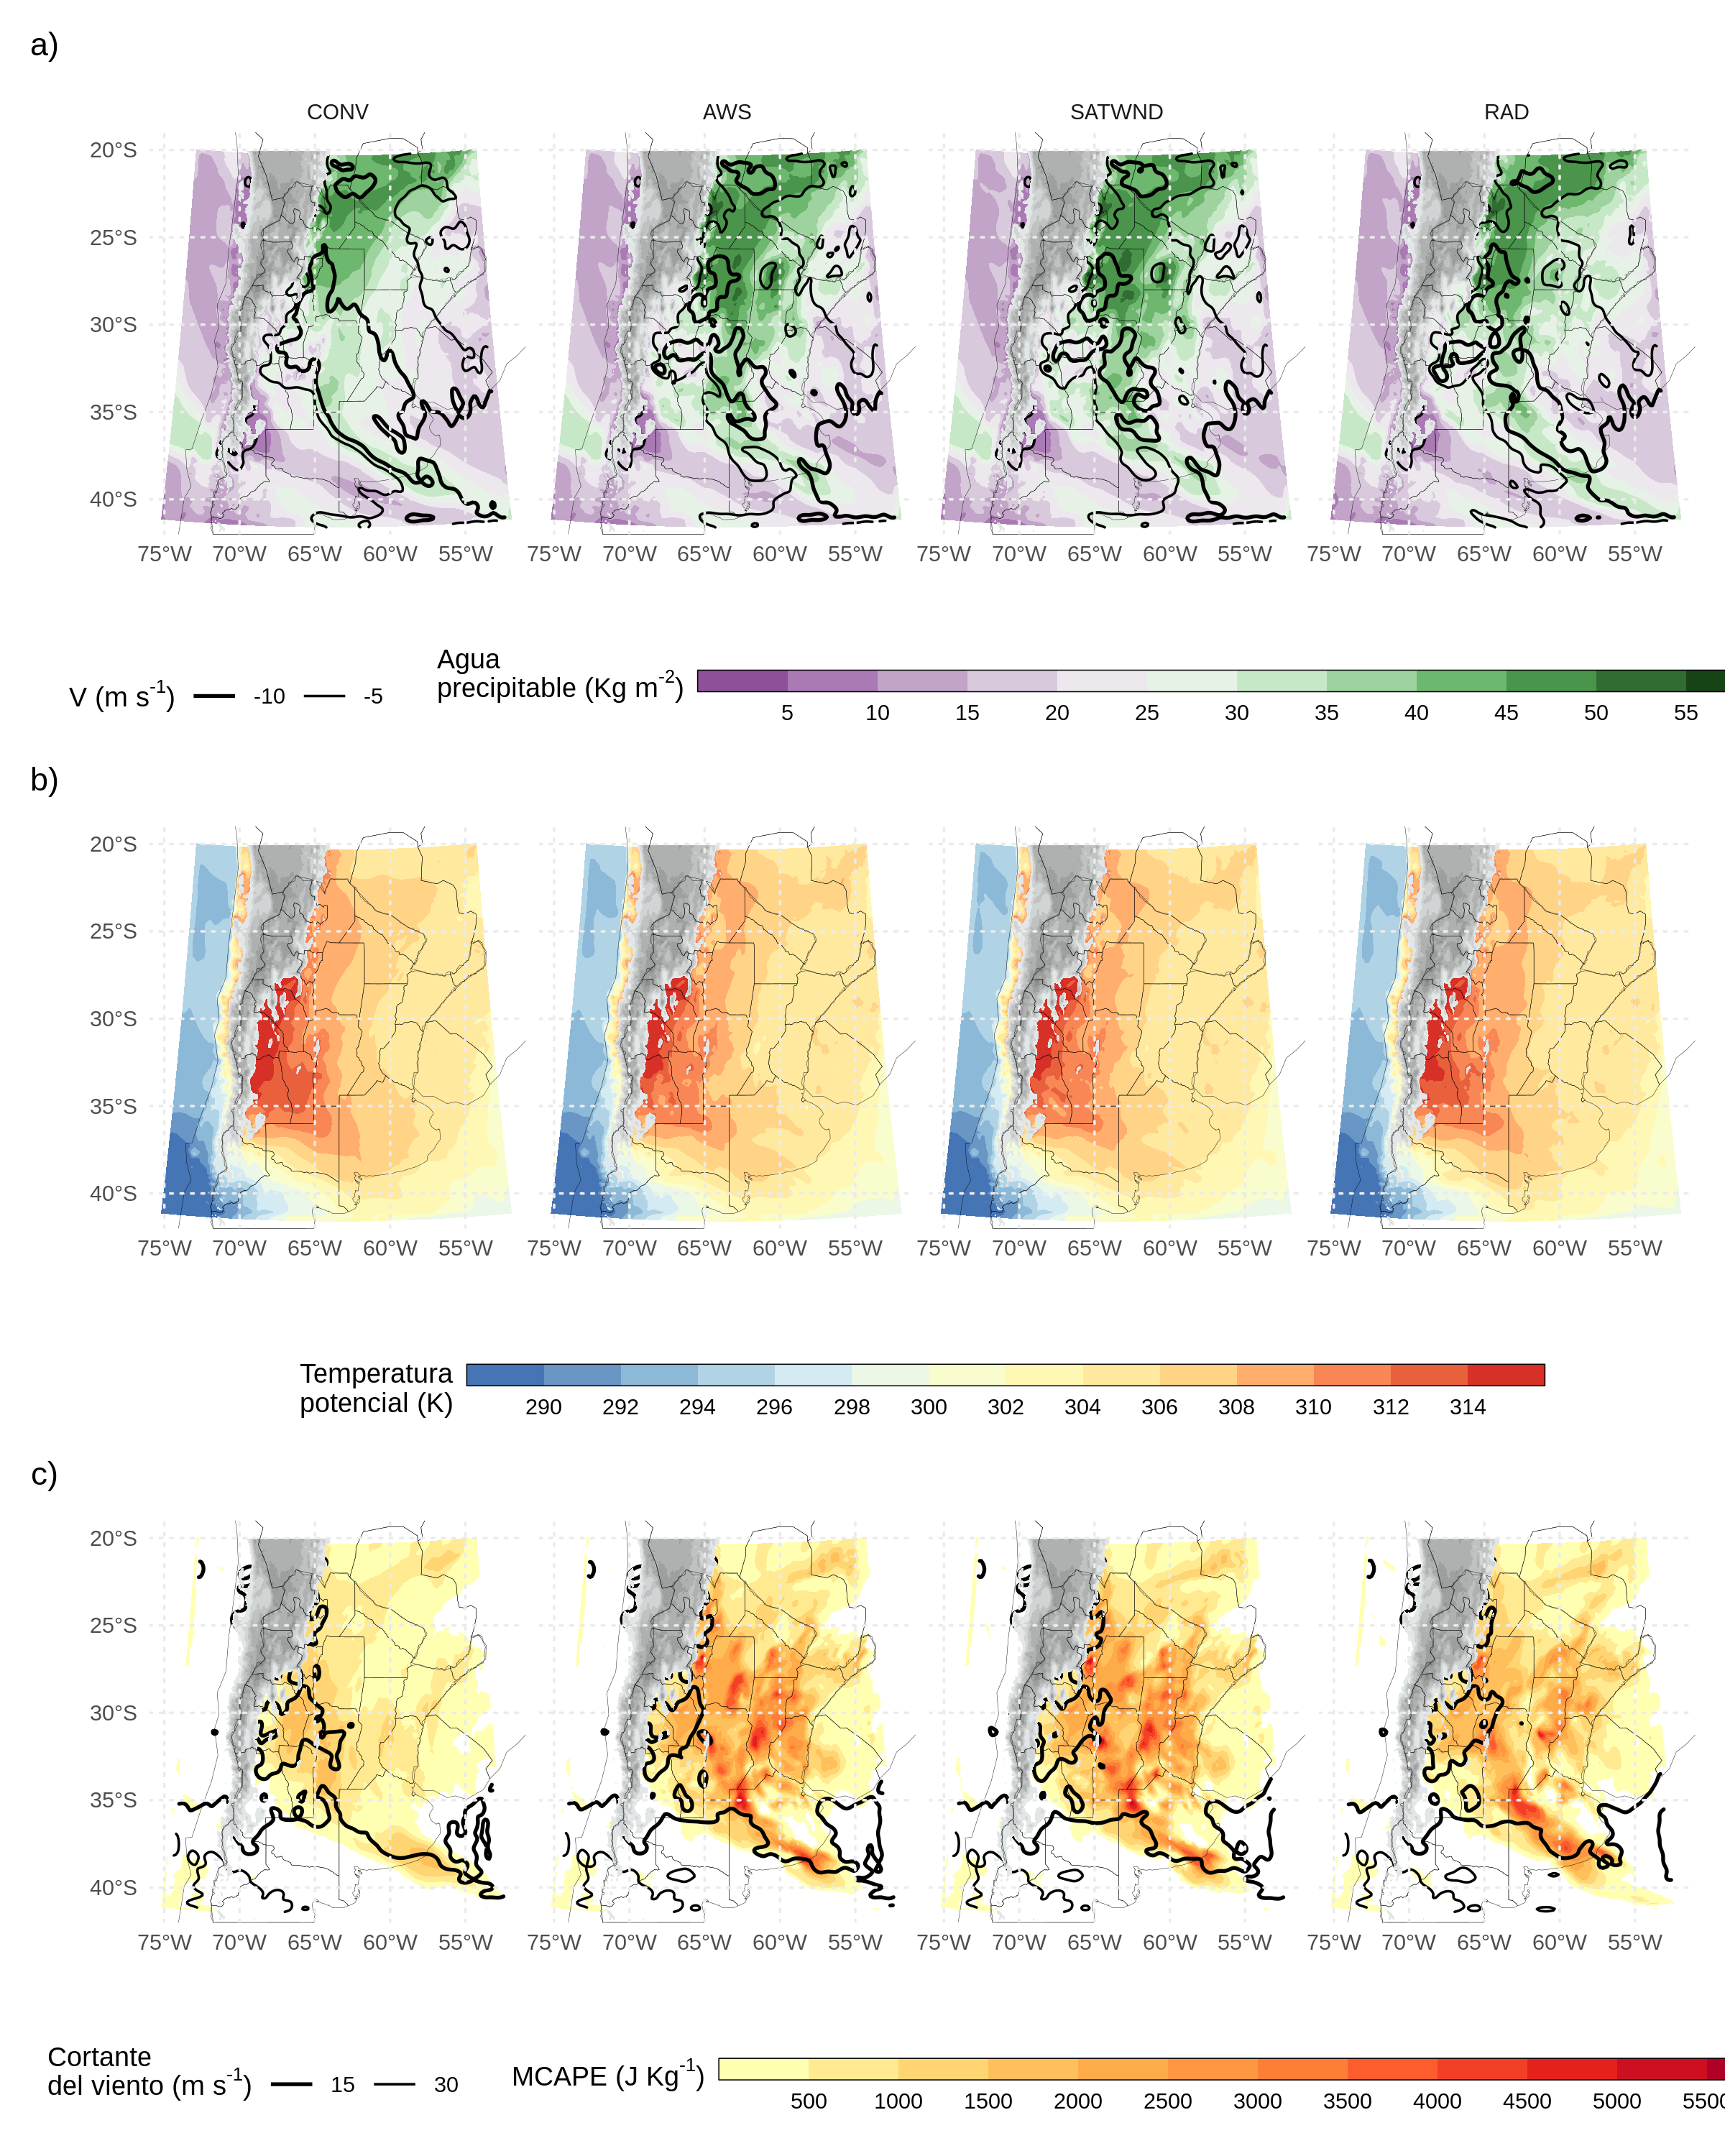
\includegraphics[width=1\linewidth,]{thesis_files/figure-latex/summary-fields-1} \caption{a) Agua precipitable (sombreada, \(kg\ m^{-2}\)) y viento medio del norte sobre los primeros 7 niveles sigma (desde la superficie hasta aproximadamente 800 hPa, contornos, \(m\ s^{-1}\)), b) Temperatura potencial media para la PBL (primeros 10 niveles sigma), y c) CAPE máxima y cortante del viento en \textasciitilde0-6 km para 15 y 30 \(m\ s^{-1}\) en cada experimento. Todos los campos corresponden a la media del ensamble del análisis para las 00 UTC del 22 de noviembre. Los contornos rellenos de color gris corresponden a la topografía de más de 1500 metros sobre el nivel del mar.}\label{fig:summary-fields}
\end{figure}
\hypertarget{validaciuxf3n-con-observaciones-independientes}{%
\subsection{Validación con observaciones independientes}\label{validaciuxf3n-con-observaciones-independientes}}

En primer lugar, se analizó el impacto de la asimilación de diferentes tipos de observación en la representación del SCM y su precipitación asociada. La figura \ref{fig:pp-hov}a muestra la precipitación acumulada horaria estimada por IMERG, y la media ajustada a la probabilidad (PM) (Clark, 2017) para la precipitación acumulada horaria del first-guess promediada entre 67\(^{\circ}\)W y 54,5\(^{\circ}\)W en función del tiempo y la latitud en los diferentes experimentos. Las precipitaciones más intensas (más de 12 \(mmh^{-1}\)) comienzan durante la tarde del 22 de noviembre y continúan durante el 23 de noviembre posterior al periodo simulado (Figura \ref{fig:pp-hov}a). En todos los experimentos, la precipitación acumulada en los pronósticos de corto plazo es subestimada. Esto es particularmente evidente en CONV (Figura \ref{fig:pp-hov}b), donde el inicio de la convección se retrasa y ocurre más al norte con respecto al inicio observado. AWS, SATWND y RAD captan mejor el momento y la ubicación de la iniciación de la convección (Figuras \ref{fig:pp-hov}c-e). AWS y RAD muestran una distribución más fragmentada en comparación con SATWND, posiblemente debido al desarrollo de una convección menos organizada durante el 22 de noviembre. Después de las 18 UTC del 22 de noviembre, RAD muestra mejoras en la tasa de precipitación y su distribución en comparación con los otros experimentos como resultado de un desarrollo de la convección más intenso.


\begin{figure}

{\centering 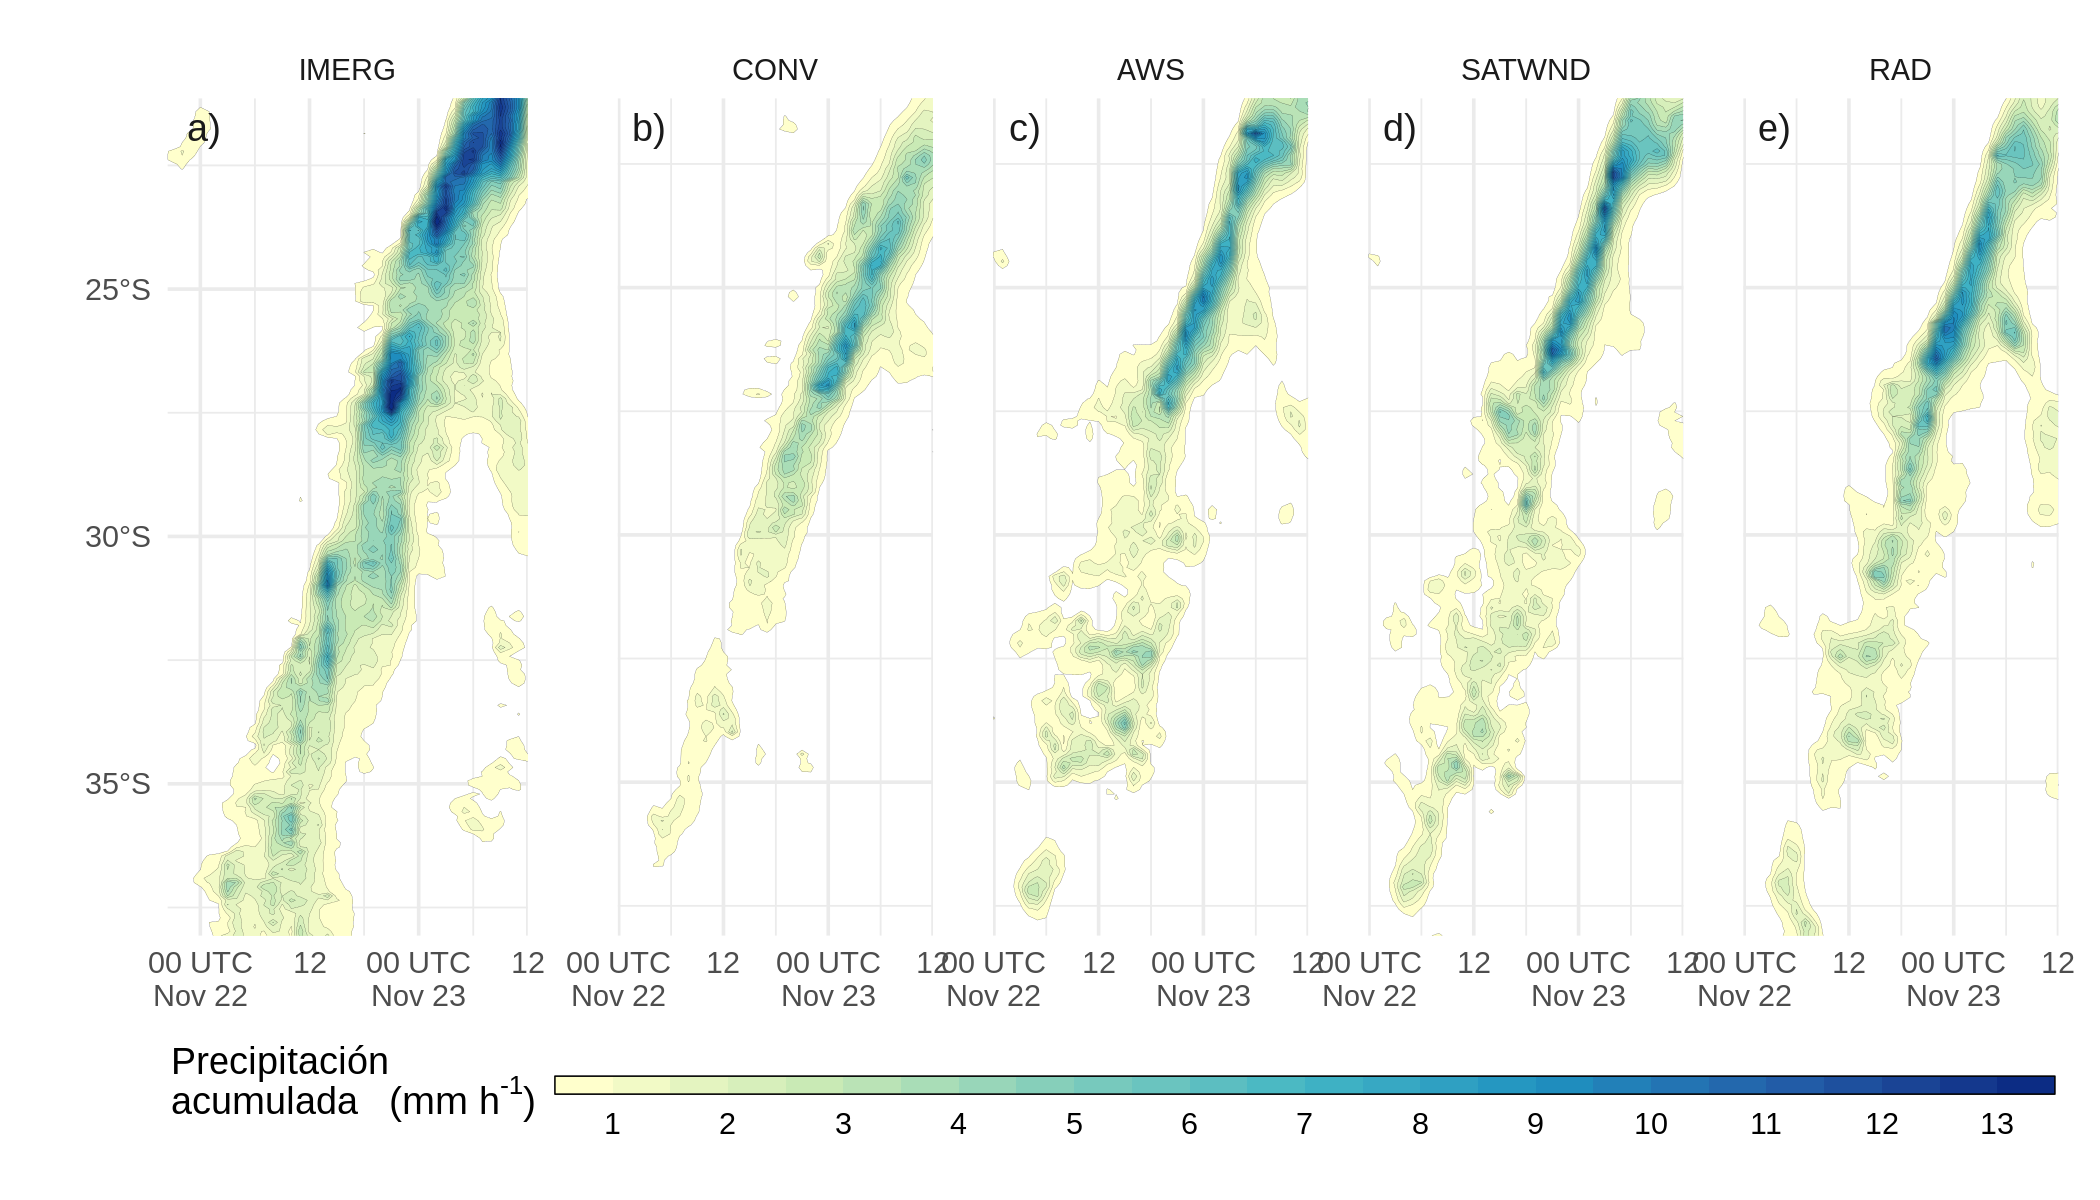
\includegraphics{thesis_files/figure-latex/pp-hov-1} 

}

\caption{Diagrama de Hövmoller de la media ajustada a la probabilidad de la precipitación acumulada horaria para cada banda de latitud estimada por IMERG (izquierda) y simulada (derecha) por cada experimento, promediada en un rango de longitudes entre 67\(^{\circ}\)W y 54,5\(^{\circ}\)W. Los contornos se dibujan cada 0,5 \(mm^{-1}\), comenzando en 0,5 \(mm^{-1}\).}\label{fig:pp-hov}
\end{figure}
El FSS se calcula para cuantificar la coincidencia espacial entre la precipitación observada y la precipitación acumulada horaria simulada por el first-guess de los diferentes experimentos (Figura \ref{fig:fss}). Para cada umbral y escala espacial, se aplica la ecuación \eqref{eq:eq11} en ventanas móviles de 6 horas a lo largo del periodo del experimento. Todos los experimentos muestran valores similares de FSS durante el inicio de la convección antes de las 06 UTC del 22 de noviembre, excepto RAD, que obtiene mejores resultados que el resto de los experimentos durante este periodo. Esto indica que las observaciones de radiancia tienen un impacto positivo en el análisis. El FSS de CONV es el más bajo en comparación con el resto de los experimentos y las diferencias son mayores durante la fase madura del SCM. AWS y SATWND muestran FSSs similares, lo que indica que la asimilación del viento estimado por satélites tiene poco impacto en la representación de la precipitación para este caso de estudio. La asimilación de radiancias conduce a una mejora general de la representación de la precipitación pronosticada a una hora, sobre todo para el umbral de 25 mm durante el periodo de mayor precipitación durante 22 de noviembre (Figura \ref{fig:fss}b,d). La mejora también es importante en la fase de desarrollo del SCM (entre las 00 y las 12 UTC del 22 de noviembre y también para escalas espaciales superiores a 500 km, no mostradas).


\begin{figure}
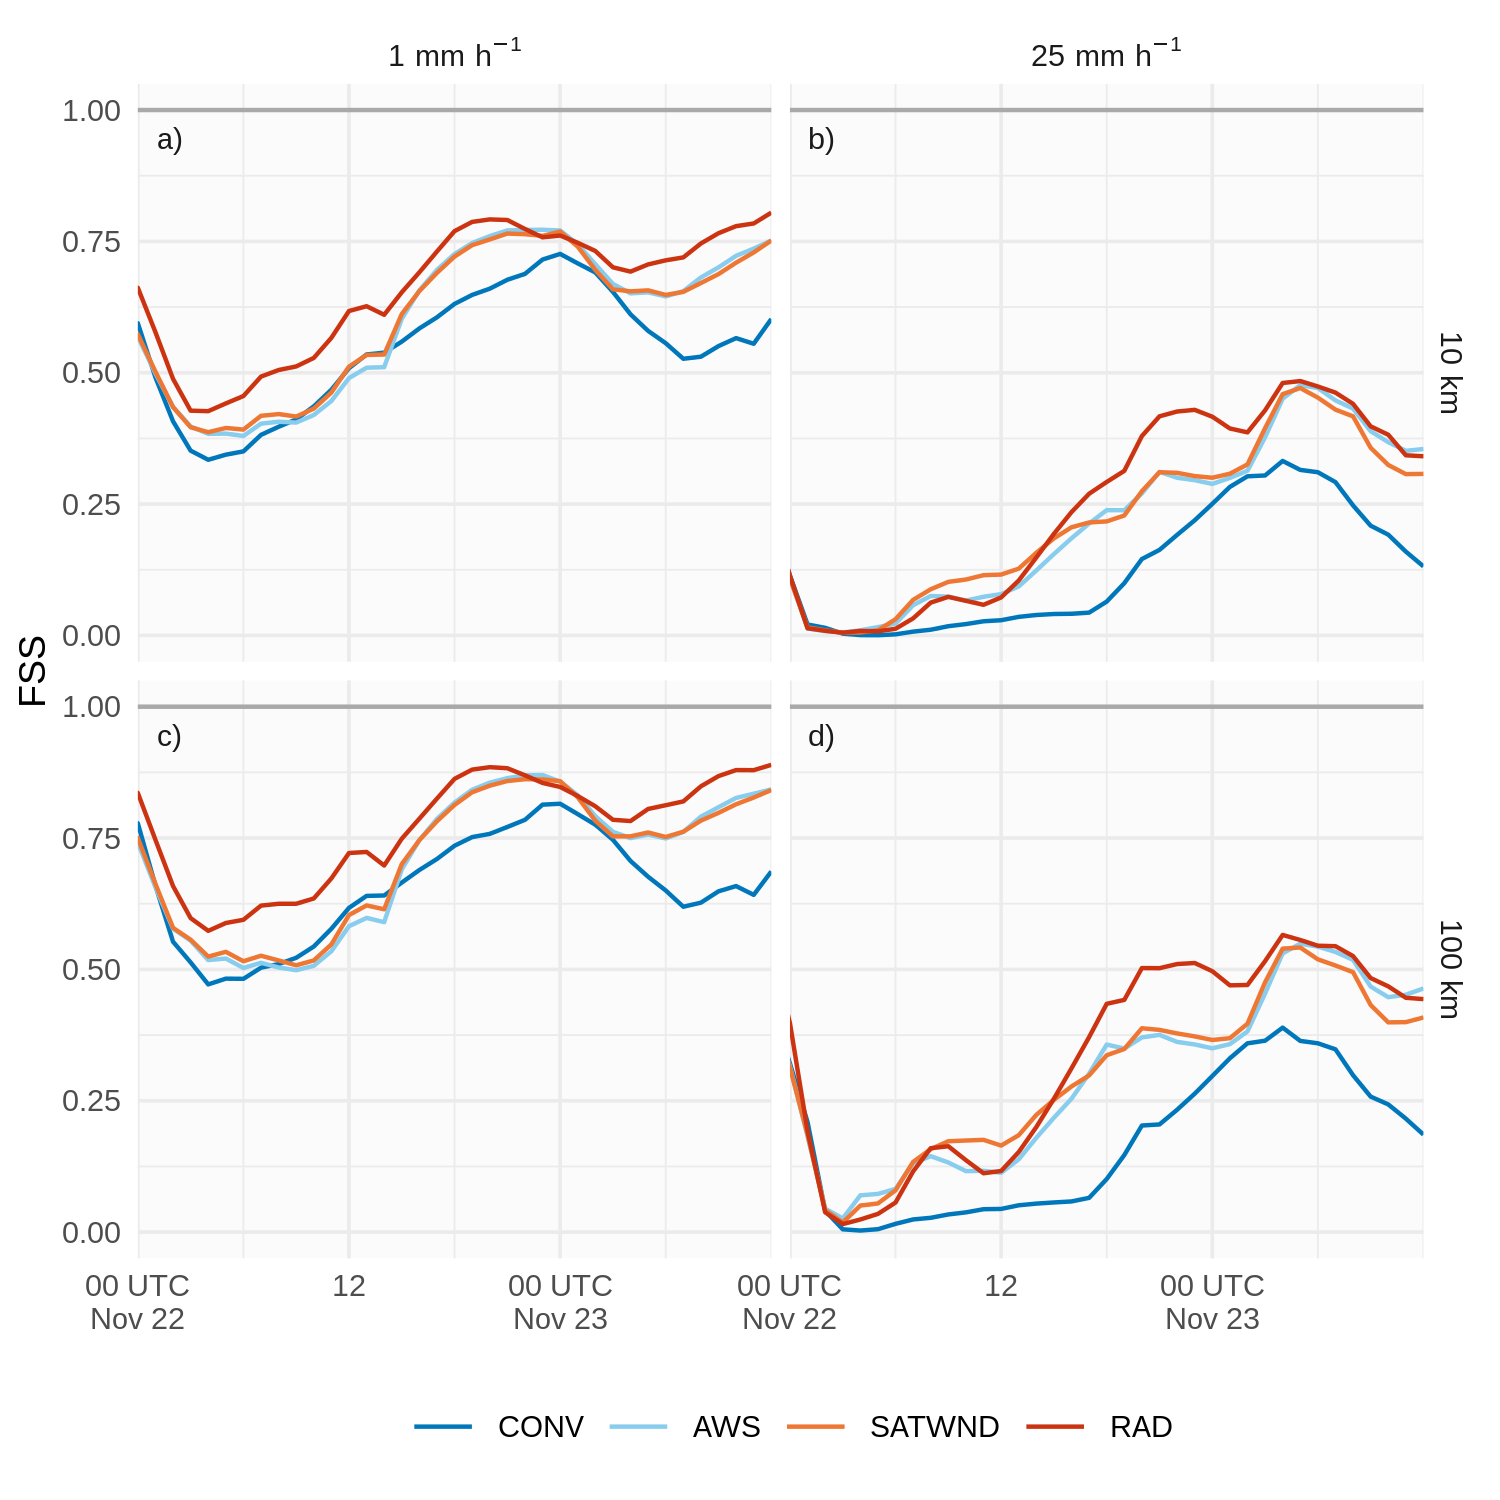
\includegraphics{thesis_files/figure-latex/fss-1} \caption{FSS calculado sobre la precipitación acumulada a 1 hora en una ventana móvil de 6 horas para umbrales de 1 mm (a y c) y 25 mm (b y d), en escalas de 10 km (a y b) y 100 km (c y d), para el campo preliminar de los experimentos CONV (línea azul), AWS (línea celeste), SATWND (línea naranja) y RAD (línea roja).}\label{fig:fss}
\end{figure}
Para complementar el análisis, la Figura \ref{fig:dbz-mean} muestra la reflectividad máxima observada en la columna vertical (COLMAX) y el COLMAX de la media del ensamble para los experimentos CONV y RAD en diferentes momentos entre las 10 y las 19 UTC del 22 de noviembre. Estos experimentos fueron elegidos porque representan el análisis con el mínimo (CONV) y el máximo (RAD) número de observaciones asimiladas. Además, son los experimentos con peor (CONV) y mejor (RAD) desempeño en cuanto a la habilidad para pronosticar la precipitación a una hora (Figura \ref{fig:fss}). En general, ninguno de los pronósticos de corto alcance capta los detalles finos de la distribución de la reflectividad. Esto es esperable si se tiene en cuenta la resolución horizontal del modelo (10 km), que no es suficiente para representar adecuadamente la intensidad de la banda convectiva asociada al SCM. RAD representa mejor las características observadas del sistema mostrando un SCM más fuerte y organizado que CONV, sobre el centro del dominio a las 10 y 13 UTC (primera y segunda columnas en la Figura \ref{fig:dbz-mean}). Las celdas convectivas que se inician después de las 16 UTC a lo largo del frente cálido en la parte noreste del dominio son bien captadas por ambos experimentos, pero están mejor representadas en términos de intensidad en RAD. Además, CONV capta la ubicación del SCM, pero la convección parece estar menos organizada y ser mucho más débil que en RAD. Antes y después de los tiempos mostrados en la Figura \ref{fig:dbz-mean}, la concordancia entre la localización de las celdas convectivas observadas y las simuladas en los experimentos es bastante buena en las regiones donde se dispone de datos de radar, especialmente para RAD.

Finalmente, la Figura \ref{fig:soundings} muestra el RMSE y el bias calculados comparando los experimentos con los datos de radiosondeos durante las misiones de observación intensiva durante RELAMPAGO, IOP 7 del 15 al 21 UTC de noviembre (incluyendo 30 radiosondeos), e IOP 8 del 14 al 20 UTC de noviembre (incluyendo 22 radiosondeos).

El IOP 7 (Figuras \ref{fig:soundings}a-d) proporciona una buena caracterización del entorno preconvectivo durante el primer día de nuestros experimentos. La zona donde se realizaron las observaciones se caracterizó por cielos mayoritariamente despejados y un flujo de norte en niveles bajos asociado a una advección cálida y húmeda. En general, los experimentos muestran un RMSE y un bias similares para todas las variables. Las observaciones de EMA lograron reducir el RMSE para la temperatura y la temperatura del punto de rocío y un bias seco en la PBL. Sin embargo, en esta región (Figura \ref{fig:dominio}b) y para este periodo, los incrementos generados por EMAs en el análisis (Figura \ref{fig:UV-diff}d) degradan el viento zonal entre 7 y 12 km aumentando el bias y el RMSE (Figura \ref{fig:soundings}c).


\begin{figure}
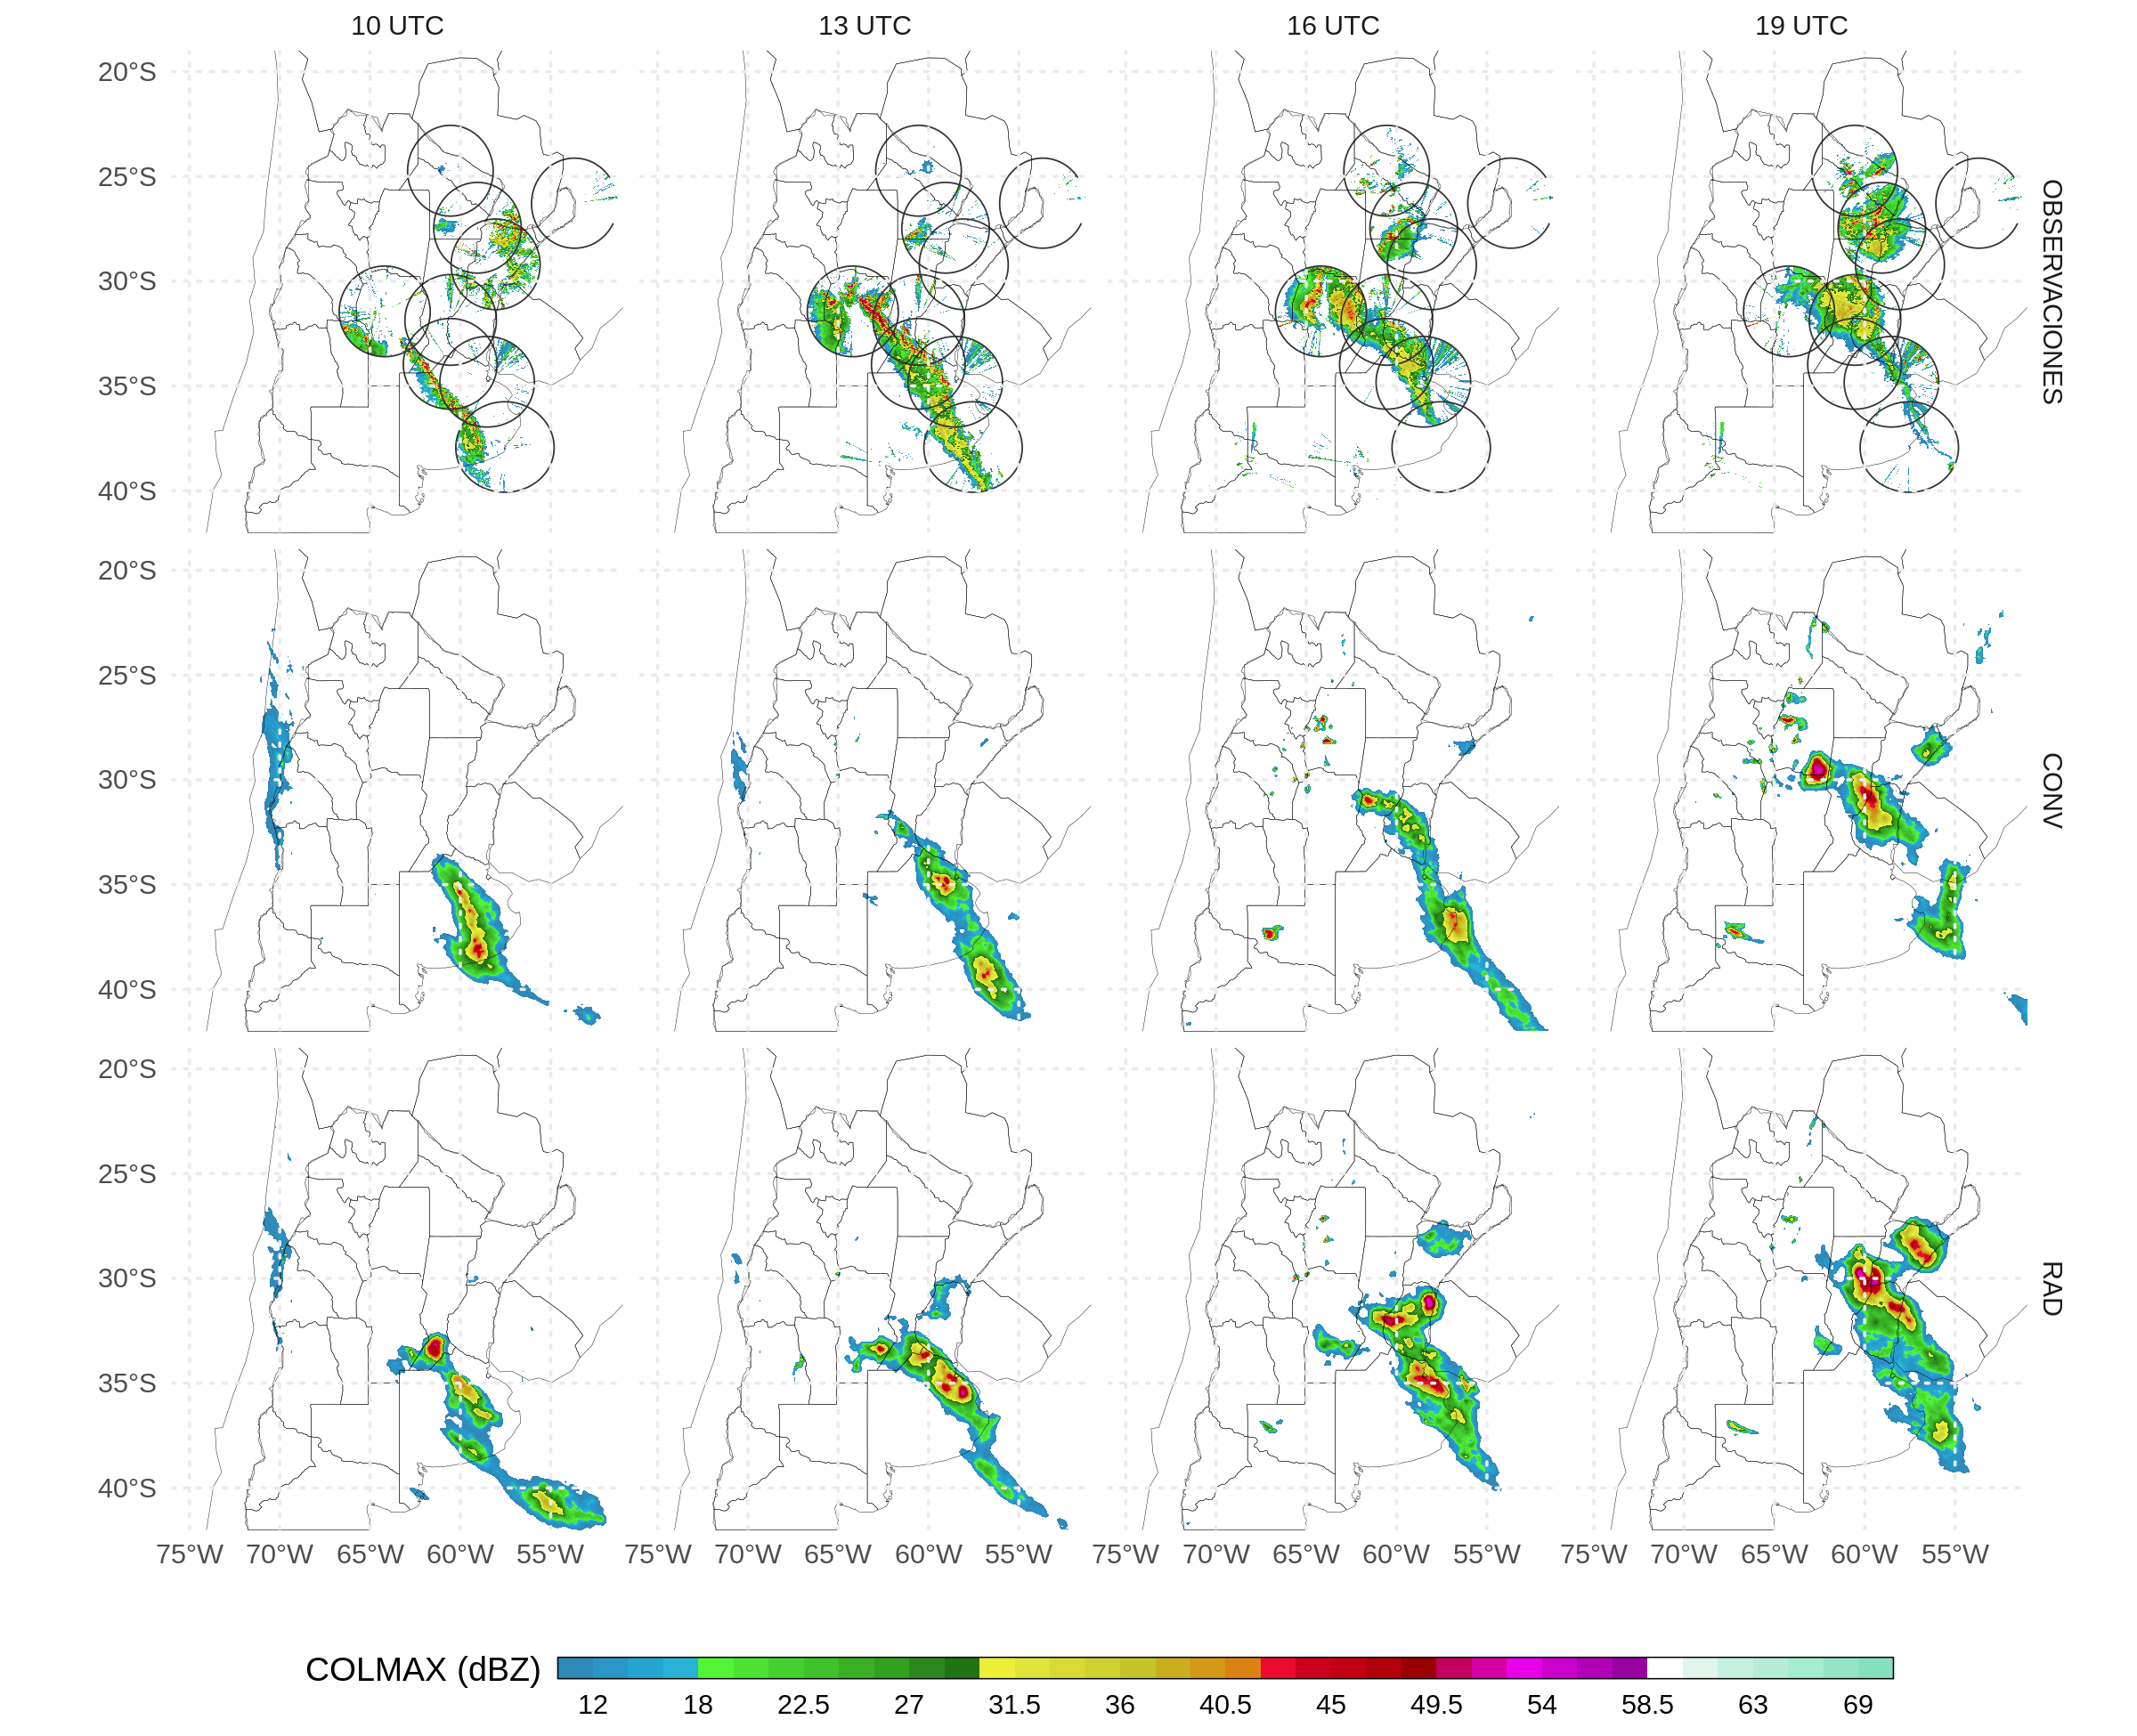
\includegraphics[width=1\linewidth,]{thesis_files/figure-latex/dbz-mean-1} \caption{Reflectividad máxima en la columna (COLMAX en \(dBZ\)), observada (fila superior) y pronósticada a 1 hora por los experimentos CONV (segunda fila) y RAD (tercera fila) a las 10 UTC (primera columna), 13 UTC (segunda columna), 16 UTC (tercera columna) y 19 UTC (cuarta columna) del 22 de noviembre de 2018. Los círculos negros en la primera fila muestran el rango de observación de cada radar.}\label{fig:dbz-mean}
\end{figure}
Durante el IOP 8 (Figuras \ref{fig:soundings}e-h), la zona densamente observada se encontraba detrás del SCM, lo suficientemente alejada del sistema como para no estar directamente afectada por su circulación de mesoescala. Esta zona también estaba detrás del frente frío y se veía afectada por advección fría en niveles bajos. La asimilación de observaciones en AWS, SATWND y RAD reduce el bias frío y el RMSE para la temperatura entre 5 y 12 km y el RMSE en la PBL en comparación con CONV (Figura \ref{fig:soundings}e). La reducción del bias y del RMSE también es importante para la temperatura del punto de rocío (Figura \ref{fig:soundings}f), siendo SATWND el que muestra el mayor impacto, seguido de AWS y RAD. El viento zonal está sobreestimado en los análisis y sólo RAD muestra una mejora con respecto a CONV en la troposfera alta (Figura \ref{fig:soundings}g). En niveles bajos el viento meridional (Figura \ref{fig:soundings}g) presenta un bias negativo, indicando una subestimación del viento del sur detrás del frente frío principalmente en AWS, SATWND, y RAD. De hecho, los bias en niveles bajos en estos experimentos son mayores que en el experimento CONV, lo que indica un efecto negativo de las observaciones asimiladas (posiblemente asociado al efecto de EMA).


\begin{figure}

{\centering 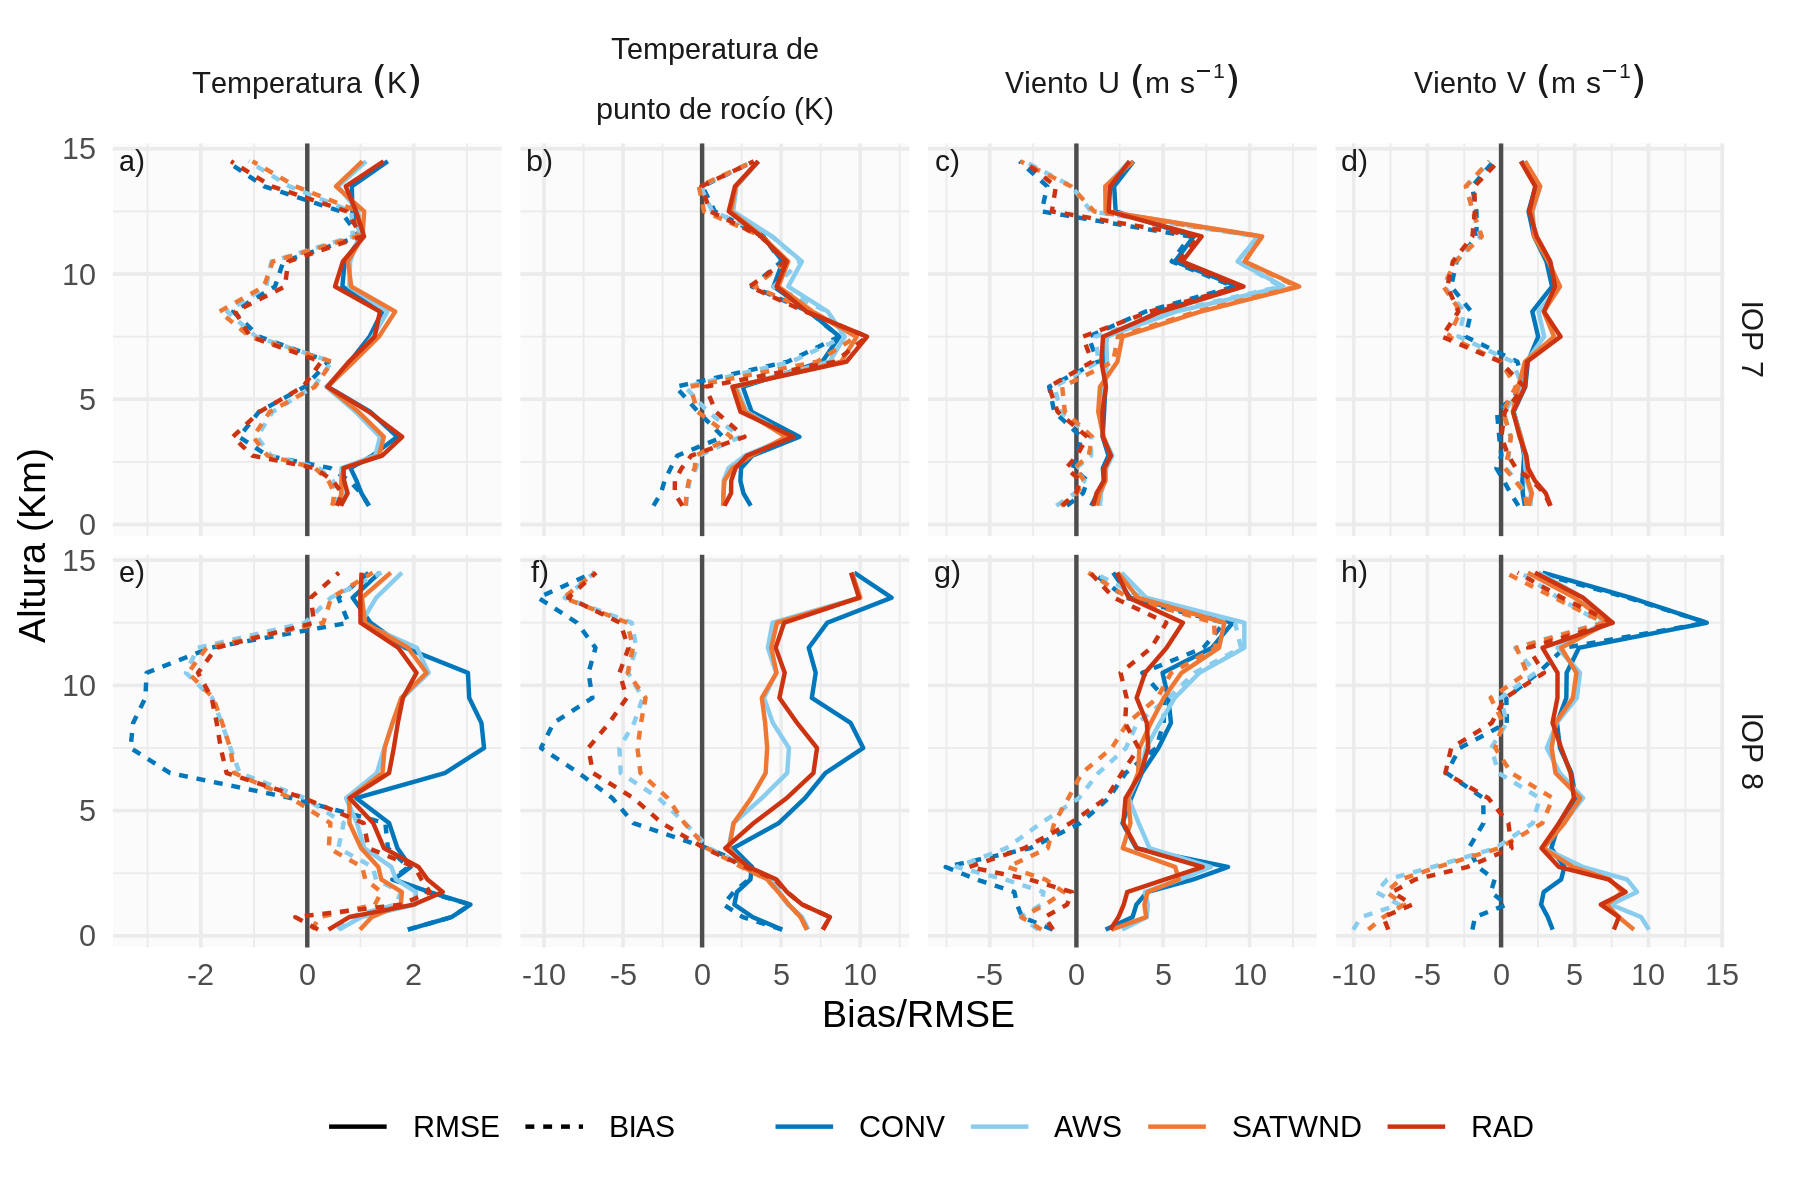
\includegraphics{thesis_files/figure-latex/soundings-1} 

}

\caption{RMSE (línea sólida) y Bias (línea discontinua) de a) la temperatura (\(K\)), b) la temperatura del punto de rocío (\(K\)), c) el viento u (\(m\ s^{-1}\)) y d) el viento v (\(m\ s^{-1}\)) calculados comparando el análisis de cada experimento con los sondeos de RELAMPAGO durante el IOP 7 y el IOP 8. La línea azul corresponde a CONV, la línea celeste a AWS, SATWND se representa con una línea naranja y RAD con una línea roja.}\label{fig:soundings}
\end{figure}
\hypertarget{conclusiones}{%
\section{Conclusiones}\label{conclusiones}}

En este capítulo se investiga el impacto de los diferentes sistemas de observación en el desempeño de un sistema de asimilación de datos regional de mesoescala basado en ensambles. Este caso de estudio corresponde a un SCM masivo que se desarrolló sobre el sur de Sudamérica el 22 de noviembre de 2018 durante la campaña de campo de RELAMPAGO. En particular, se explora el impacto en la calidad del análisis de la asimilación de las observaciones superficiales frecuentes y espacialmente densas provenientes de estaciones automáticas, los vientos estimados por satélite y las radiancias de cielo claro sensores a bordo de satélites polares.

En primer lugar, se evaluó la consistencia del ensamble para analizar la concordancia concordancia entre la dispersión del ensamble y los errores de observación con respecto a la distancia entre la media del ensamble y las observaciones. Mientras que las desviaciones de las observaciones convencionales son coherentes con la dispersión del ensamble y los errores de observación asumidos, las desviaciones de las observaciones de viento estimado por satélitee y radiancias son menores de lo esperado. Esto último podría ser el resultado de una sobreestimación de los errores de observación que se suele introducir para evitar el impacto perjudicial en el análisis de las observaciones de baja calidad.

En general todos los tipos de observación considerados (es decir, las estaciones meteorológicas automáticas, los vientos estimados por satélites y las radiancias de cielo claro procedentes de los satélites de órbita polar) mejoran la calidad del análisis y del pronóstico a corto plazo de precipitación cuando se comparan los resultados obtenidos al asimilar solo las observaciones de la red de observación convencional. En cuanto al análisis, las observaciones de las estaciones meteorológicas automáticas, que tienen una alta resolución espacial y temporal, produjeron impactos principalmente dentro de la PBL, pero que ocasionalmente se extienden por toda la troposfera durante los períodos en los que la convección húmeda es más intensa dentro del dominio. Estas observaciones también ayudaron a reducir el bias cálido y seco presente en el modelo, produciendo un análisis más cercano a ERA5. Durante el periodo preconvectivo, la asimilación de la temperatura de superficie, la temperatura del punto de rocío y el viento meridional mejoró el análisis en niveles bajos en comparación con los sondeos de la campaña RELAMPAGO. En particular, cuando se asimilan estas observaciones, el contenido de agua precipitable y la circulación meridional en niveles bajos condujeron a un aumento de la convección profunda y de la precipitacón intensa acercando el análisis a lo observado.

También se encontraron resultados positivos al asimilar las observaciones de radiancia, que produjeron un mejor desarrollo de la convección y de su circulación de salida asociada, principalmente durante la fase madura del SCM, lo que condujo a un aumento de la precipitación acumulada en comparación con el caso en el que no se asimilan estas observaciones. Sin embargo, estas observaciones debilitaron el impacto de las observaciones de las estaciones meteorológicas automáticas dentro de la PBL, aumentando ligeramente el bias cálido y seco del modelo. Aunque esto debe estudiarse más a fondo, podría estar relacionado con la asimilación de canales afectados por la superficie o con una corrección de bias de las observaciones subóptima. Comparando el experimento con sondeos independientes, la asimilación de radiancias mejoró el viento en niveles medios y altos.

La asimilación del viento estimado por satélite no produjo un impacto notable en el análisis. Esto se debe posiblemente al número relativamente pequeño de observaciones en niveles bajos disponibles para este caso de estudio y gran error de observación asignado durante la asimilación. Sin embargo, se observan mejoras en la distribución de la precipitación acumulada en el pronóstico a 1 hora. Es necesario realizar un análisis más exhaustivo para comprender los mecanismos que subyacen al impacto de estas observaciones en los pronósticos de mayor alcance, que será tema de análisis en el capítulo 2.

\hypertarget{impacto-de-la-asimilaciuxf3n-de-observaciones-convencionales-de-estaciones-automuxe1ticas-vientos-derivados-de-satuxe9lite-y-radianzas-de-satelites-polares-en-pronuxf3sticos-a-corto-plazo}{%
\chapter{Impacto de la asimilación de observaciones convencionales, de estaciones automáticas, vientos derivados de satélite y radianzas de satelites polares en pronósticos a corto plazo}\label{impacto-de-la-asimilaciuxf3n-de-observaciones-convencionales-de-estaciones-automuxe1ticas-vientos-derivados-de-satuxe9lite-y-radianzas-de-satelites-polares-en-pronuxf3sticos-a-corto-plazo}}

En este capítulo se evaluará en impacto de la asimilación de distintas fuentes de observación en pronósticos por ensable a corto plazo inicializados a partir del análisis de los distintos experimentos descriptos en la sección \ref{config}. Estos pronósticos abarcan el periodo de iniciación, madurez y dearrollo del SCM observado durant el 22 y 23 de noviembre de 2022. Por lo tanto se analizará el impacto de la asimilación de observaciones a lo largo de los pronósticos en un contexto de convección húmeda profunda y se evaluará si las mejoras observadas en los análisis al respresentar este caso de estudio se trasladan a los pronósticos independientes.

\hypertarget{metodologuxeda-1}{%
\section{Metodología}\label{metodologuxeda-1}}

\hypertarget{configuracion-de-los-experimentos}{%
\subsection{Configuracion de los experimentos}\label{configuracion-de-los-experimentos}}

Para estudiar el impacto de la asimilación de observaciones en pronósticos independientes, se generaron pronósticos por ensambles inicializados a partir de los análisis de los experimentos previamente descriptos. Estos pronósticos toman el nombre del análisis que utilizan como condición inicial, por ejemplo el pronóstico CONV será aquel que fue incializado a partir del análisis del experimento CONV. Todos los pronósticos utilizan la misma configuración de dominio y de ensamble multifísica que los análisis. Las condiciones de borde de los miembros del ensamble se generaron añadiendo perturbaciones aleatorias al pronóstico determinístico del GFS (0.25\(^{\circ}\) de resolución horizontal y resolución temporal de 6 horas; National Centers for Environmental Prediction, National Weather Service, NOAA, U.S. Department of Commerce (2015)) como se muestra en la Figura \ref{fig:cycle-fcst}.

Los pronósticos se inicializaron a las 00 y 06 UTC del 22 de noviembre para capturar la inicialización y desarrollo del SCM y además evaluar las posibles diferencias entre los experimentos debido a la asimilación de nuevas observaciones entre las 00 y las 06 UTC. Todos los pronósticos finalizan a las 12 UTC del 23 de noviembre cuando el SCM se encuentra en el borde noroeste del dominio y ya no puede ser representado correctamente (Figura \ref{fig:caso}f).


\begin{figure}
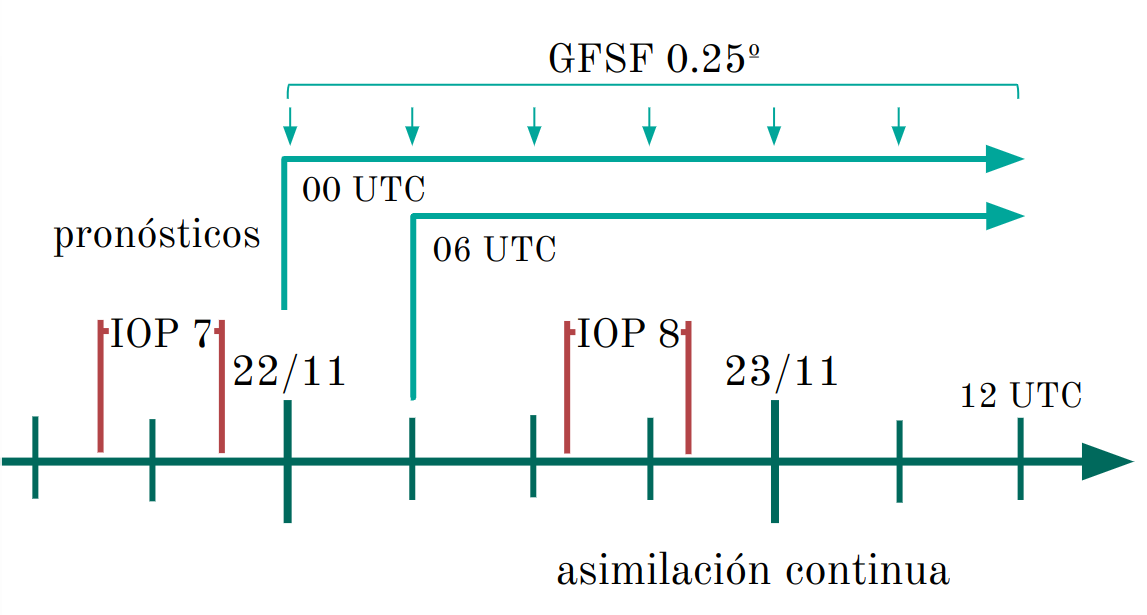
\includegraphics[width=1\linewidth,]{/home/paola.corrales/tesis_doctorado/figure/forecast_diag} \caption{Diagrama de los pronósticos por ensambles inicializados a las 00 y 06 UTC del 22 de noviembre y que corren hasta las 12 UTC del 23 de noviembre. Las condiciones de borde corresponden al pronóstico de GFS y se incorporan cada 6 horas.}\label{fig:cycle-fcst}
\end{figure}
\hypertarget{resultados-1}{%
\section{Resultados}\label{resultados-1}}

\hypertarget{prono-impacto}{%
\subsection{Impacto de las observaciones en el pronostico}\label{prono-impacto}}

Al igual que en la sección \ref{impacto-analisis}, se compararon los pronósticos con ERA5. Los perfiles de temperatura de la media del ensamble promediados espacialmente menos ERA5 a lo largo del tiempo se muestran en las Figuras \ref{fig:era5-fcst-1}. En lineas generales la temperatura por encima de 750 hPa es subestimada por los pronósticos pero esto parece ser independiente de las condiciones iniciales ya que no se ven diferencias entre los experimentos y tampoco entre la hora de inicialización de los pronósticos. En niveles bajos se observa la misma tendencia que en los análisis, los pronósticos inicializados a partir de AWS y SATWND muestran un bias cálido mucho menor que CONV gracias a las condiciones iniciales que incluyen la asimilación de observaciones de EMA. En RAD el bias cálido vuelve a aumentar ligeramente manteniendo la tendencia observada en los análisis de RAD (Figuras \ref{fig:era5-fcst-1}d y h). En niveles bajos sí se ven diferencias entre las dos inicializaciones, en particular se observan mejoras para la inicialización de las 06 UTC en los casos de AWS y SATWND, indicando que las observaciones asimiladas entre las 00 y las 06 UTC tienen un impacto positivo en la representación de la temperatura cerca de superficie que se traslada a los pronósticos.

Las diferencias entre los pronósticos y ERA5 para los perfiles promediados de humedad específica (Figuras \ref{fig:era5-fcst-2}) muestran nuevamente el bias seco presente en el modelo y que es más importante en horas nocturnas. Sin embargo es notaria la mejora en los pronósticos inicializados a partir de AWS y SATWND y RAD, en comparación con CONV. Las condiciones iniciales de los pronósticos CONV tienen un bias seco muy marcado que se mantiene a lo largo de todo el periodo de pronóstico (Figuras \ref{fig:era5-fcst-2}a y e). Las dos inicialización, en este caso, no muestran diferencias apreciables.








\begin{figure}[ht]

{\centering 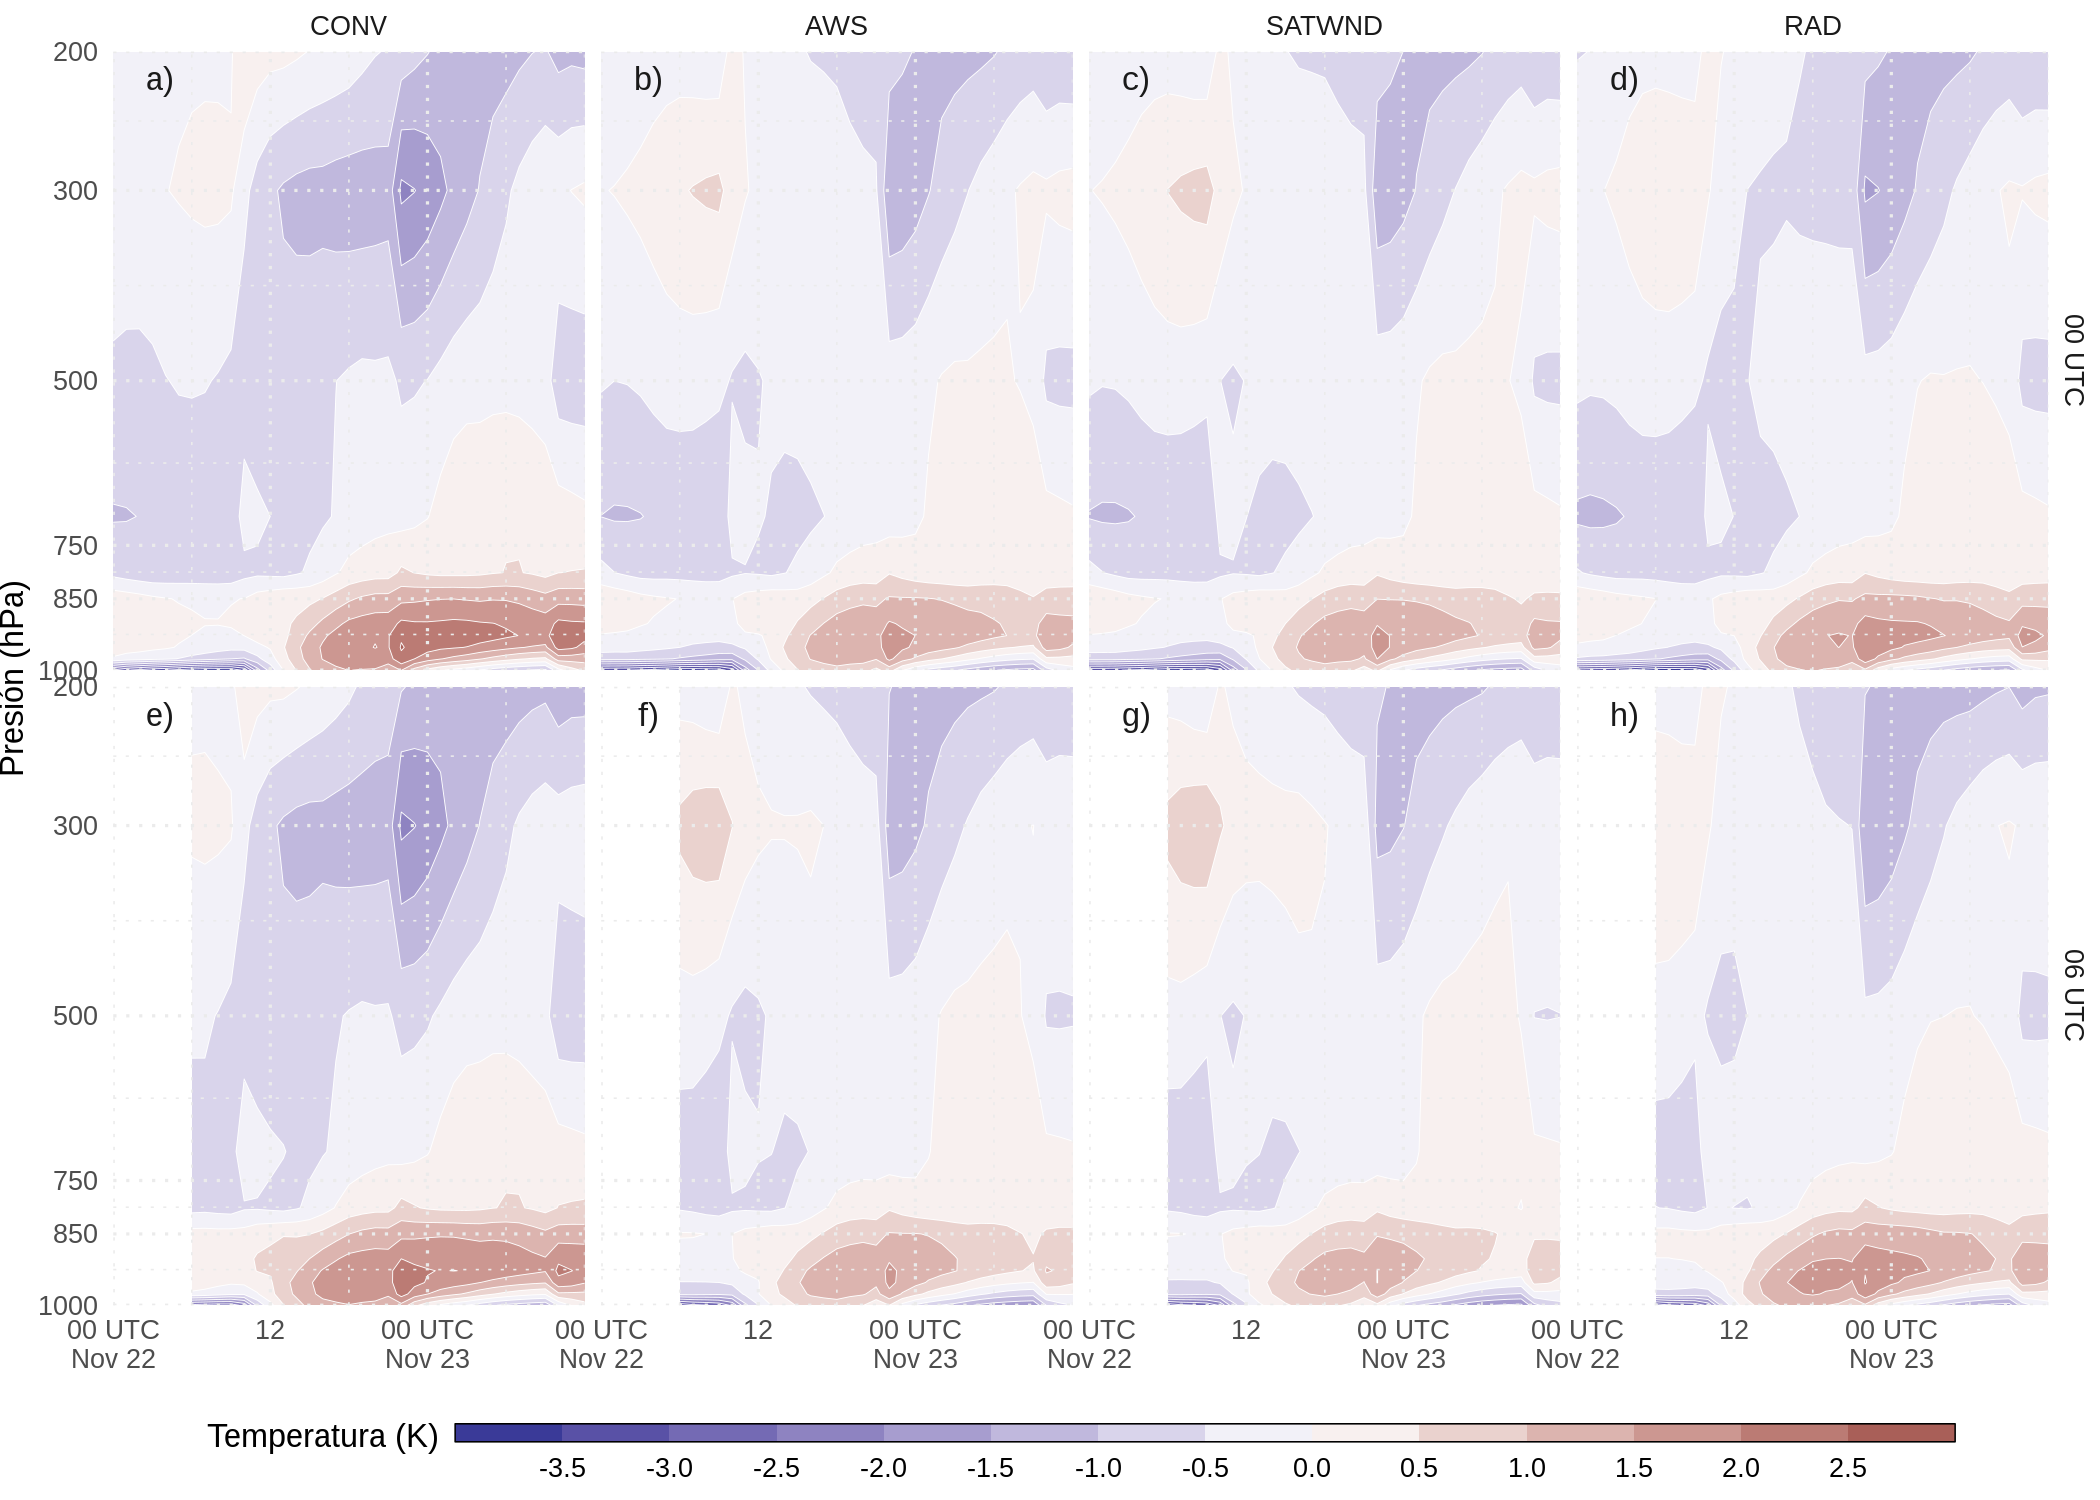
\includegraphics{thesis_files/figure-latex/era5-fcst-1} 

}

\caption{Diferencia entre la media del ensamble del pronóstico inicializado a partir de cada experimento y ERA5 de los perfiles verticales promediados espacialmente de la temperatura del aire (\(K\)) calculado sobre el dominio de validación (cuadro rojo en la Figura \ref{fig:dominio}a) para cada tiempo de pronóstico.}\label{fig:era5-fcst-1}
\end{figure}
\begin{figure}[ht]

{\centering 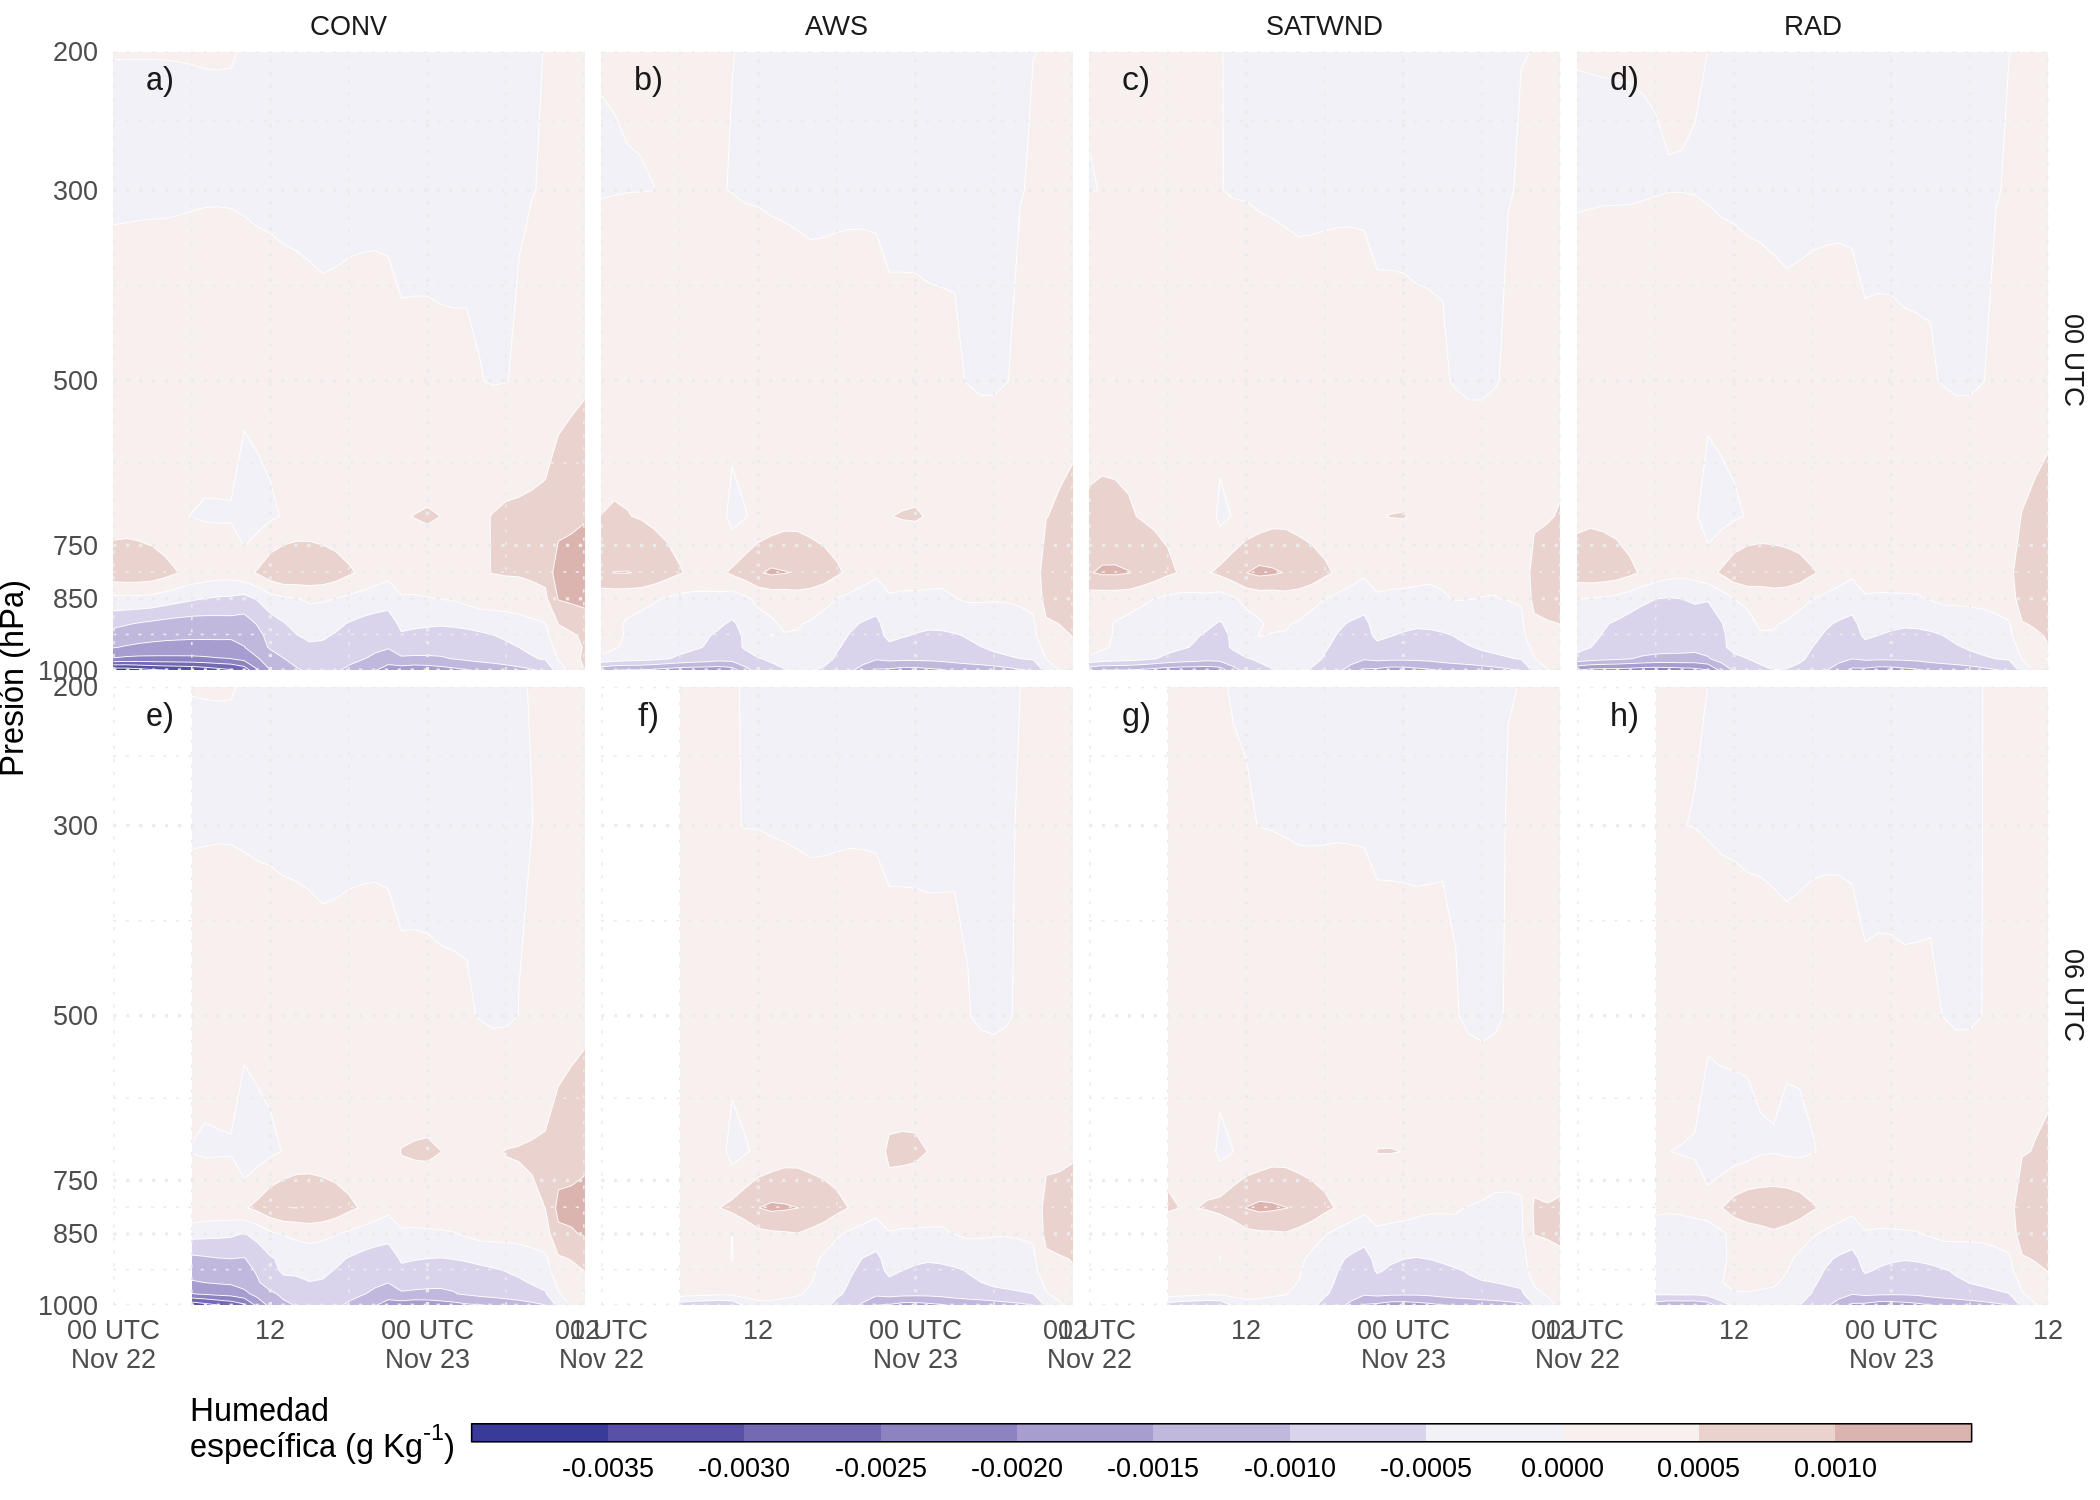
\includegraphics{thesis_files/figure-latex/era5-fcst-2} 

}

\caption{Cómo en la Figura \ref{fig:era5-fcst-1} pero para la humedad específica (\(g\ Kg^{-1}\)).}\label{fig:era5-fcst-2}
\end{figure}
\begin{figure}[ht]

{\centering 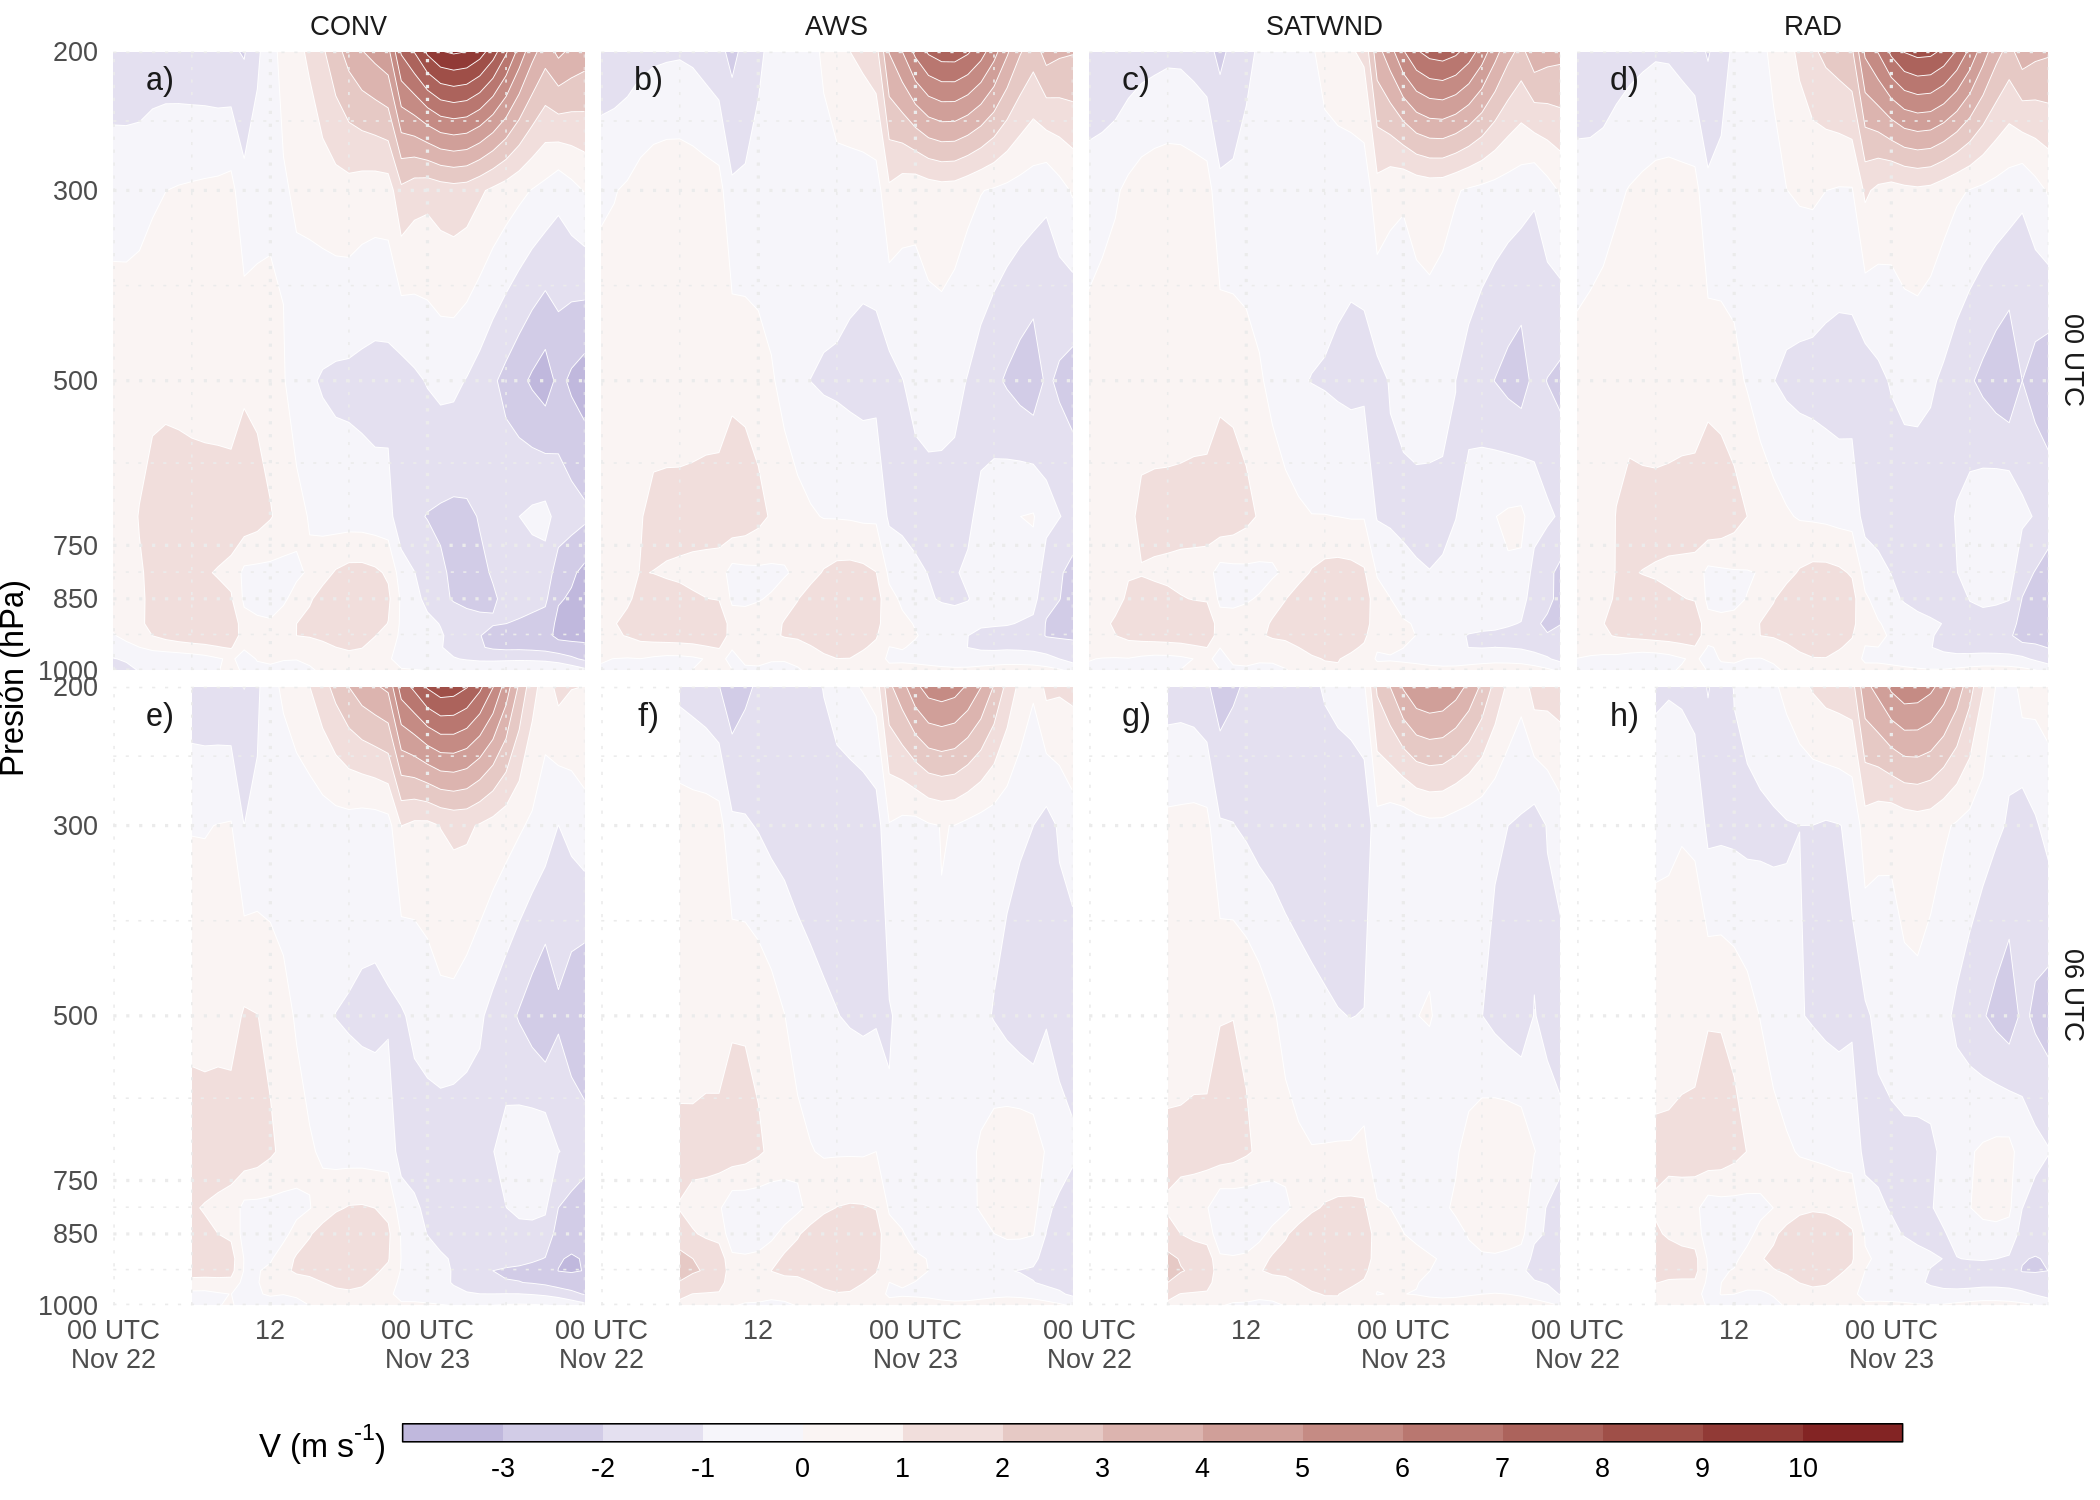
\includegraphics{thesis_files/figure-latex/era5-fcst-3} 

}

\caption{Cómo en la Figura \ref{fig:era5-fcst-1} pero para el viento meridional (\(m\ s^{-1}\)).}\label{fig:era5-fcst-3}
\end{figure}
\begin{figure}[ht]

{\centering 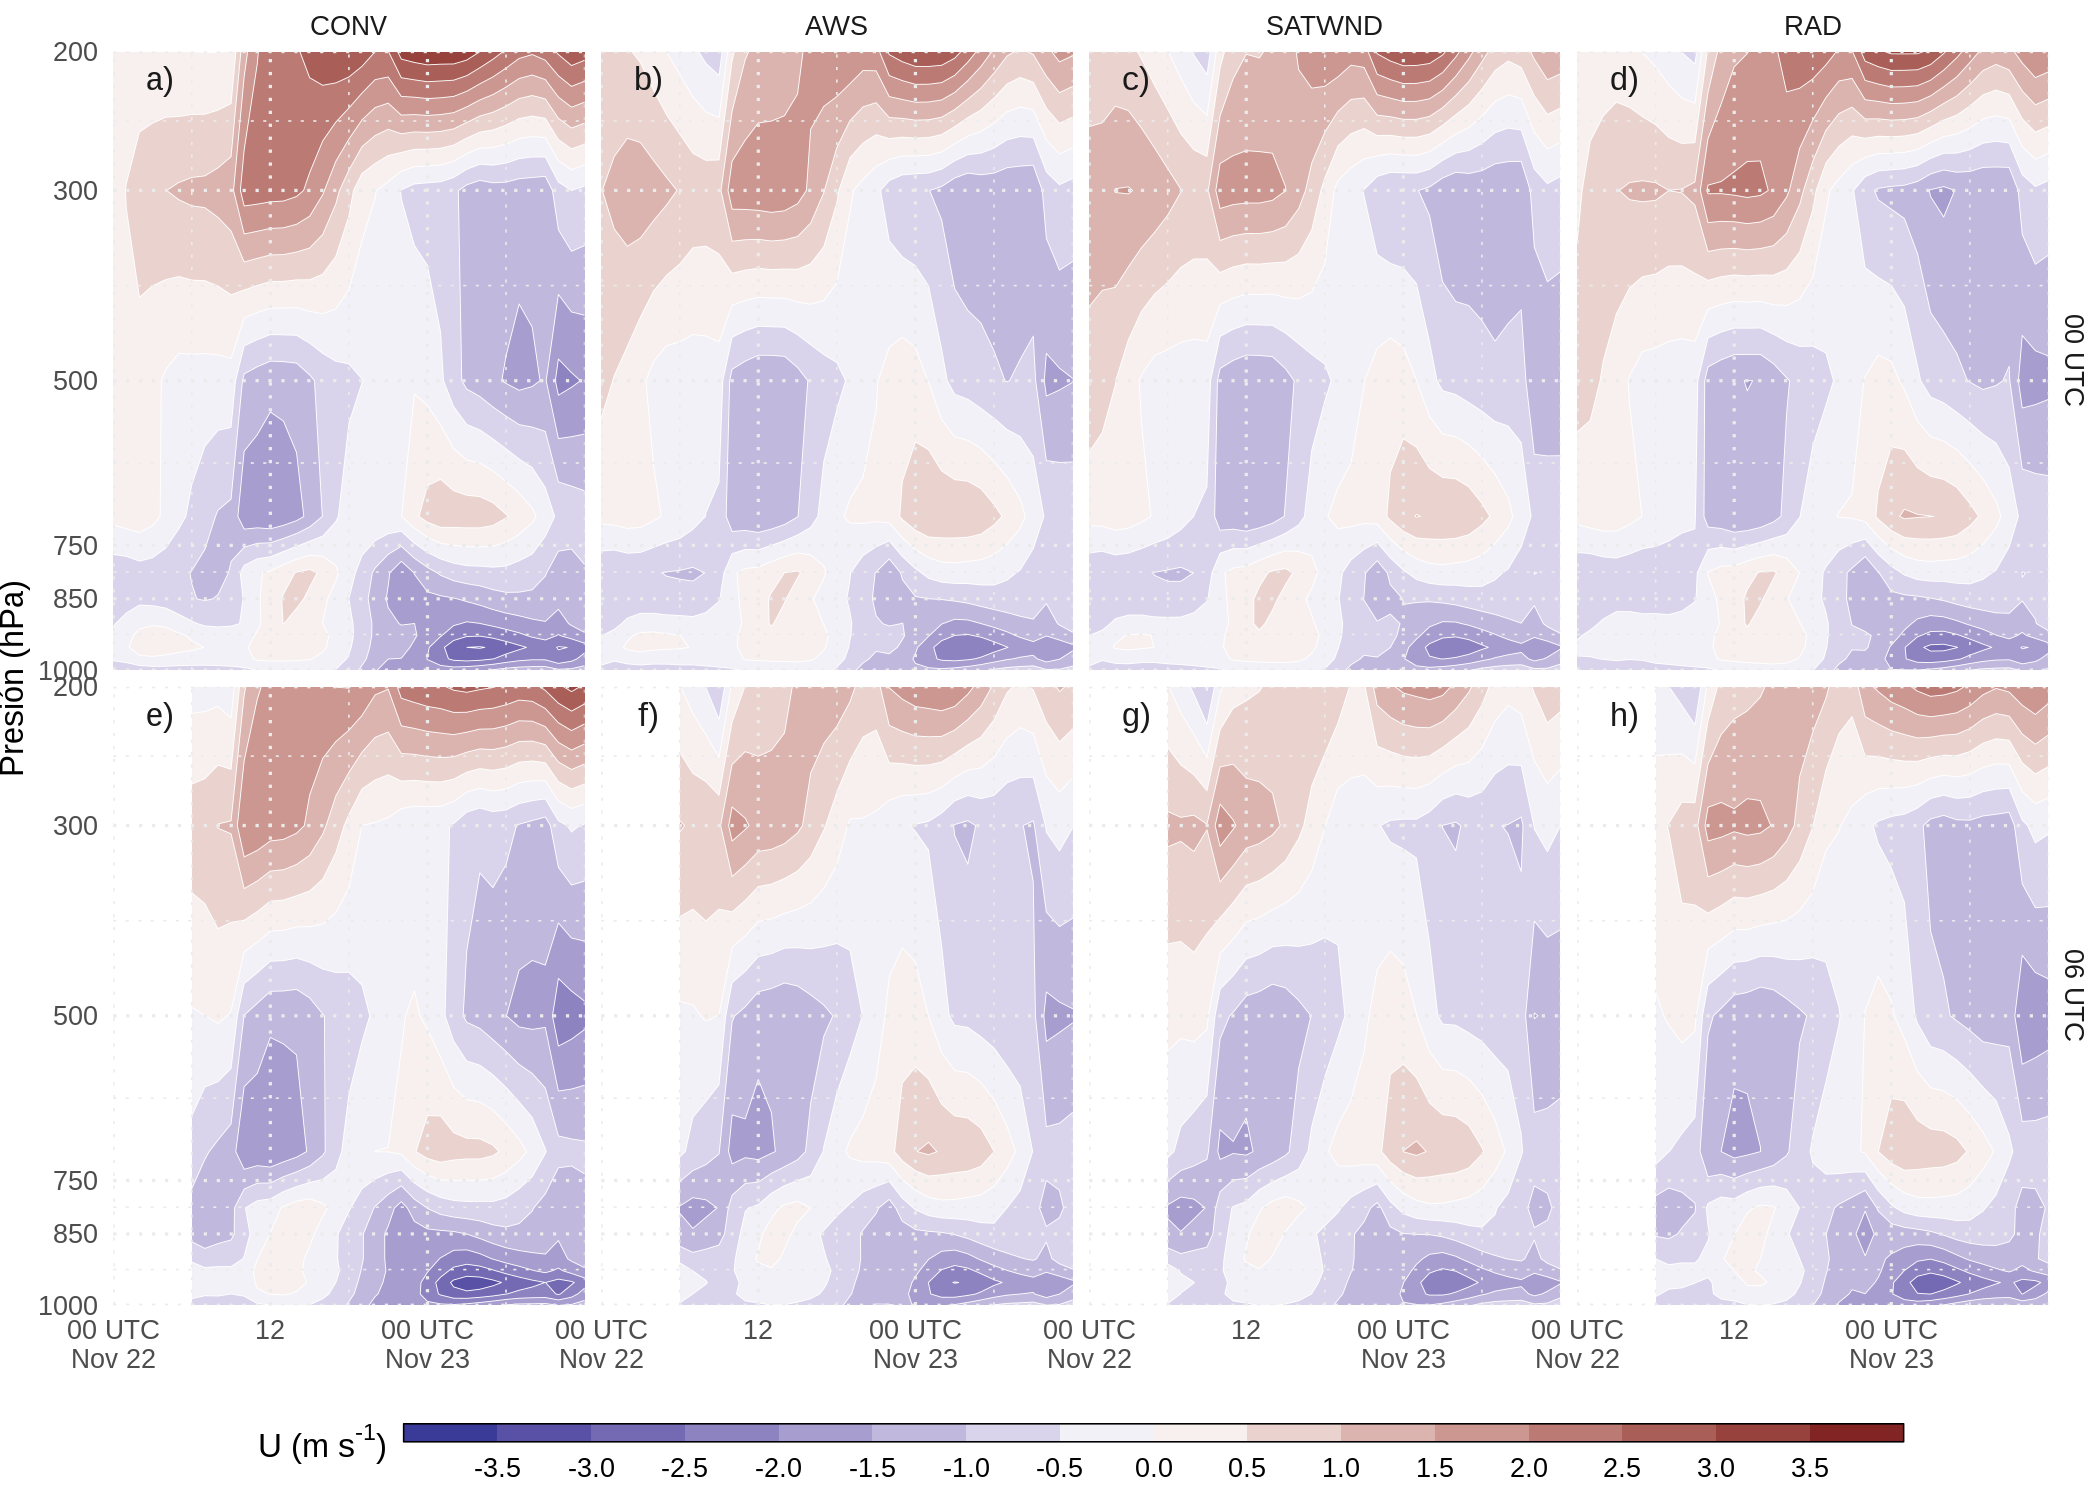
\includegraphics{thesis_files/figure-latex/era5-fcst-4} 

}

\caption{Cómo en la Figura \ref{fig:era5-fcst-1} pero para el viento zonal (\(m\ s^{-1}\)).}\label{fig:era5-fcst-4}
\end{figure}
Es interesante notar que la asimilación de radianzas que aportan información en niveles medios y altos, también produce un impacto en niveles bajos de la atmósfera. Es posible que el desarrollo nuboso que se ve influenciado por cambios de temperatura y humedad genera también cambios en la temperatura en superficie. En este caso las mayores temperaturas observadas en los pronósticos de RAD se pueden explicar por una disminución en el desarrollo de nubes (no se muestra).

La mayor diferencia en los perfiles promediados para el viento meridional se observa en niveles altos y está asociado al periodo de mayor actividad convectiva sobre el norte del dominio (Figuras \ref{fig:era5-fcst-3}). En particular SATWND es el pronóstico que mejor representa el viento meridional, particularmente en el pronóstico inicializado a las 06 UTC (Figura \ref{fig:era5-fcst-3}g). Esto es particularmente intererante ya que el impacto de las observaciones de viento derivadas de satélite asimiladas en el experimento SATWND era marginal comparado al impacto de otra fuentes de observaciones. Sin embargo los pronósticos inicializados con condiciones inciales que incluye información de viento derivado de satélite representan mejor el viento meridional aún en los periodos de mayor convección. Si se analizan los experimentos individualmente alrededor de las 00 UTC del 23 de noviembre, se observa que SATWND presenta mayor convergencia en niveles bajos y mayor divergencia en niveles altos cuando se lo compara con RAD. Esto podría indica que la convección en SATWND es más intensa.

Algo similar se observa en la diferencia entre perfiles vericales del viento zonal en las Figuras \ref{fig:era5-fcst-3}. Los pronósticos inicializados a partir de los experimentos AWS, SATWND y RAD muestran una mejor representación del viento zonal en todos los niveles. Sin embargo las observaciones de satelites polares parecen generar un impacto negativo en las condiciones iniciales de RAD que se traslada al pronóstico aumentando la diferencia respecto de ERA5.

\hypertarget{verificacion-de-los-pronuxf3sticos-de-precipitaciuxf3n}{%
\subsection{Verificacion de los pronósticos de precipitación}\label{verificacion-de-los-pronuxf3sticos-de-precipitaciuxf3n}}

Para cuantificar la habilidad de los pronósticos a 30 y 36 hs para representar la precipitación se calculó el FSS sobre ensambles de los pronósticos en ventanas móviles de 6 horas para los mismos umbrales y escalas espaciales usados para la precipitación acumulada horaria del campo preliminar (Figura \ref{fig:fssfcst}). Los pronósticos de CONV generan valores muy bajos de FSS en comparación con los experimentos que incluyen otras fuentes de observaciones lo que indica una subestimación de la precipitación en todas las escalas. AWS, SATWND y RAD muestran mejoras en los valores de FSS, especialmente para el umbral de 25 mm (Figura \ref{fig:fssfcst}b, d). Además, la inicialización de las 06 UTC muestra mejores resultados en todos los experimentos que los pronósticos inicializados a las 00 UTC, lo que pone de relieve el impacto positivo de las observaciones asimiladas entre las 00 y las 06 UTC en la representación de la precipitación.

Las observaciones de viento derivadas de satélite muestran un impacto claramente positivo en los pronósticos, a diferencia de lo que se observó al comparar el pronóstico a 1 hora con observaciones independientes en la verificación de los análisis. Esto evidencia el desarrollo de convección más intensa y es coherente con lo analizado en la sección \ref{prono-impacto} Por el contrario, las radiancias tuvieron un impacto neutro a ligeramente negativo en los pronósticos inicializados a las 00 y 06 UTC. Si bien existen muchos posibles motivos por el que los pronósticos inicializados a partir de RAD se degradan con el tiempo, es posible que la asimilación de observaciones asociadas a canales afectados por la superficie esté contribuyendo a la degradación de la capa límite en el análisis y, posteriormente, en los pronósticos. Por ejemplo, Lim et al. (2014) observó un impacto limitado al asimilar las observaciones de AIRS y atribuye este resultado al uso de canales superficiales en los que las incertidumbres asociadas a la emisividad de la superficie son grandes.


\begin{figure}
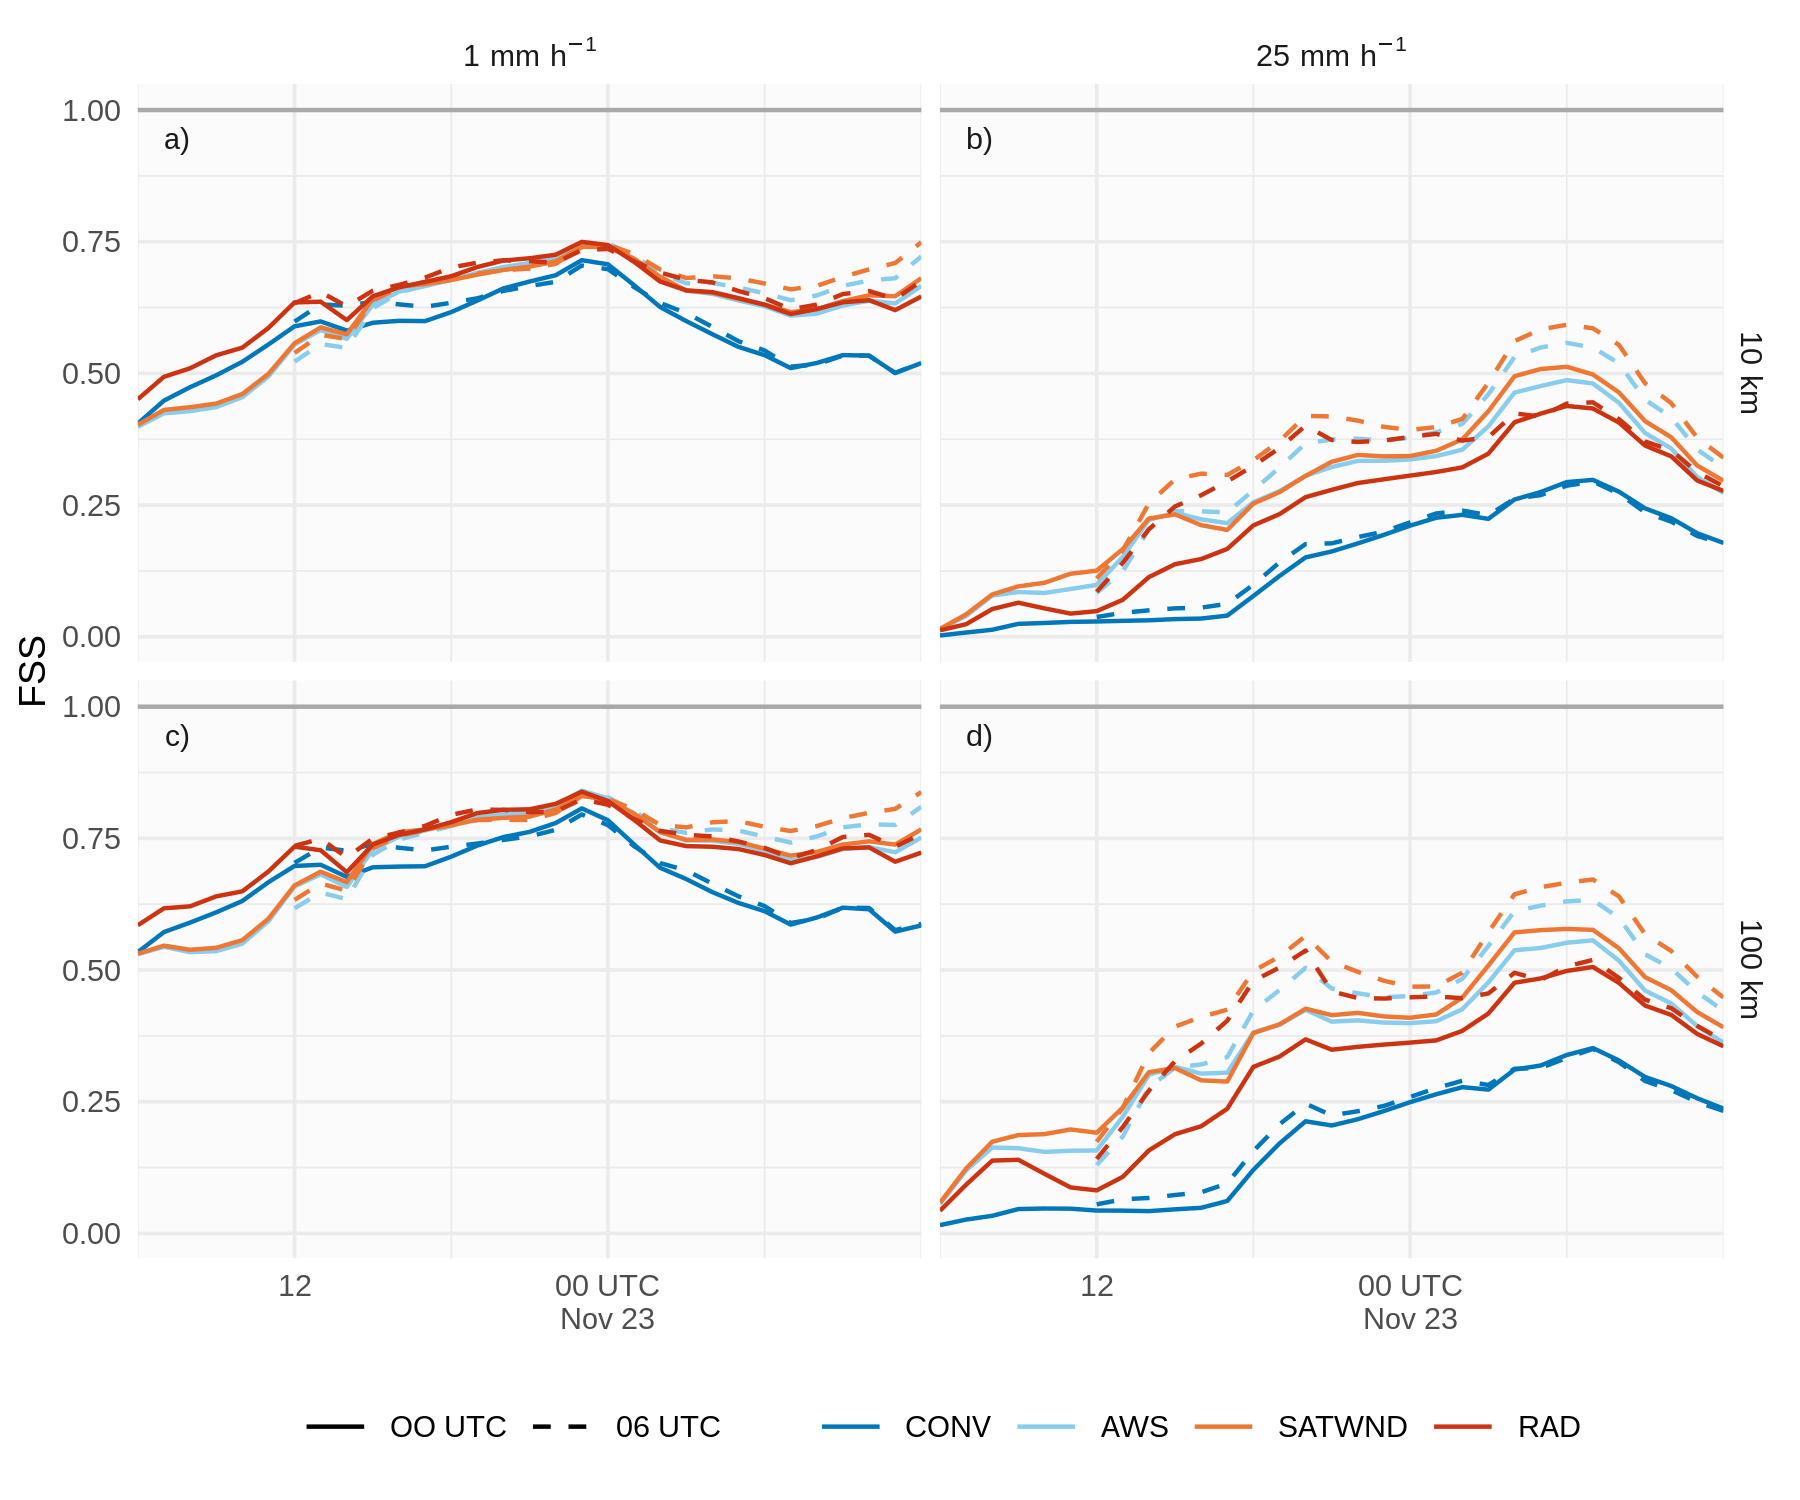
\includegraphics{thesis_files/figure-latex/fssfcst-1} \caption{FSS calculado sobre la precipitación acumulada a 1 hora en una ventana móvil de 6 horas para umbrales de 1 mm (a y c) y 25 mm (b y d), en escalas de 10 km (a y b) y 100 km (c y d), para los pronósticos inicializados a partir de los experimentos CONV (línea azul), AWS (línea celeste), SATWND (línea naranja) y RAD (línea roja) a las 00 UTC (línea sólida) y 06 UTC (linea punteada) del 22 de noviembre.}\label{fig:fssfcst}
\end{figure}
El porcentaje de área cubierta por precipitación superior a determinados umbrales se muestra en la Figura \ref{fig:area}. Nuevamente, los pronósticos muestran una importante subestimación de la precipitación media, en particular CONV. El área sombreada que muestra el área máxima estimada sobre todos los miembros del ensamble se acerca al área estimada por IMERG, sin embargo todos los experimentos y sobre todo en el umbral de \(1 mmh^{-1}\), la precipitación se adelantan en el tiempo. Los pronósticos inicializados a partir de CONV subestiman el área cubierta por precipitación durante el periodo más activio y luego la sobreestiman durante el 23 de noviembre cuando ya no se observa precipitación intensa dentro del dominio de estudio.


\begin{figure}
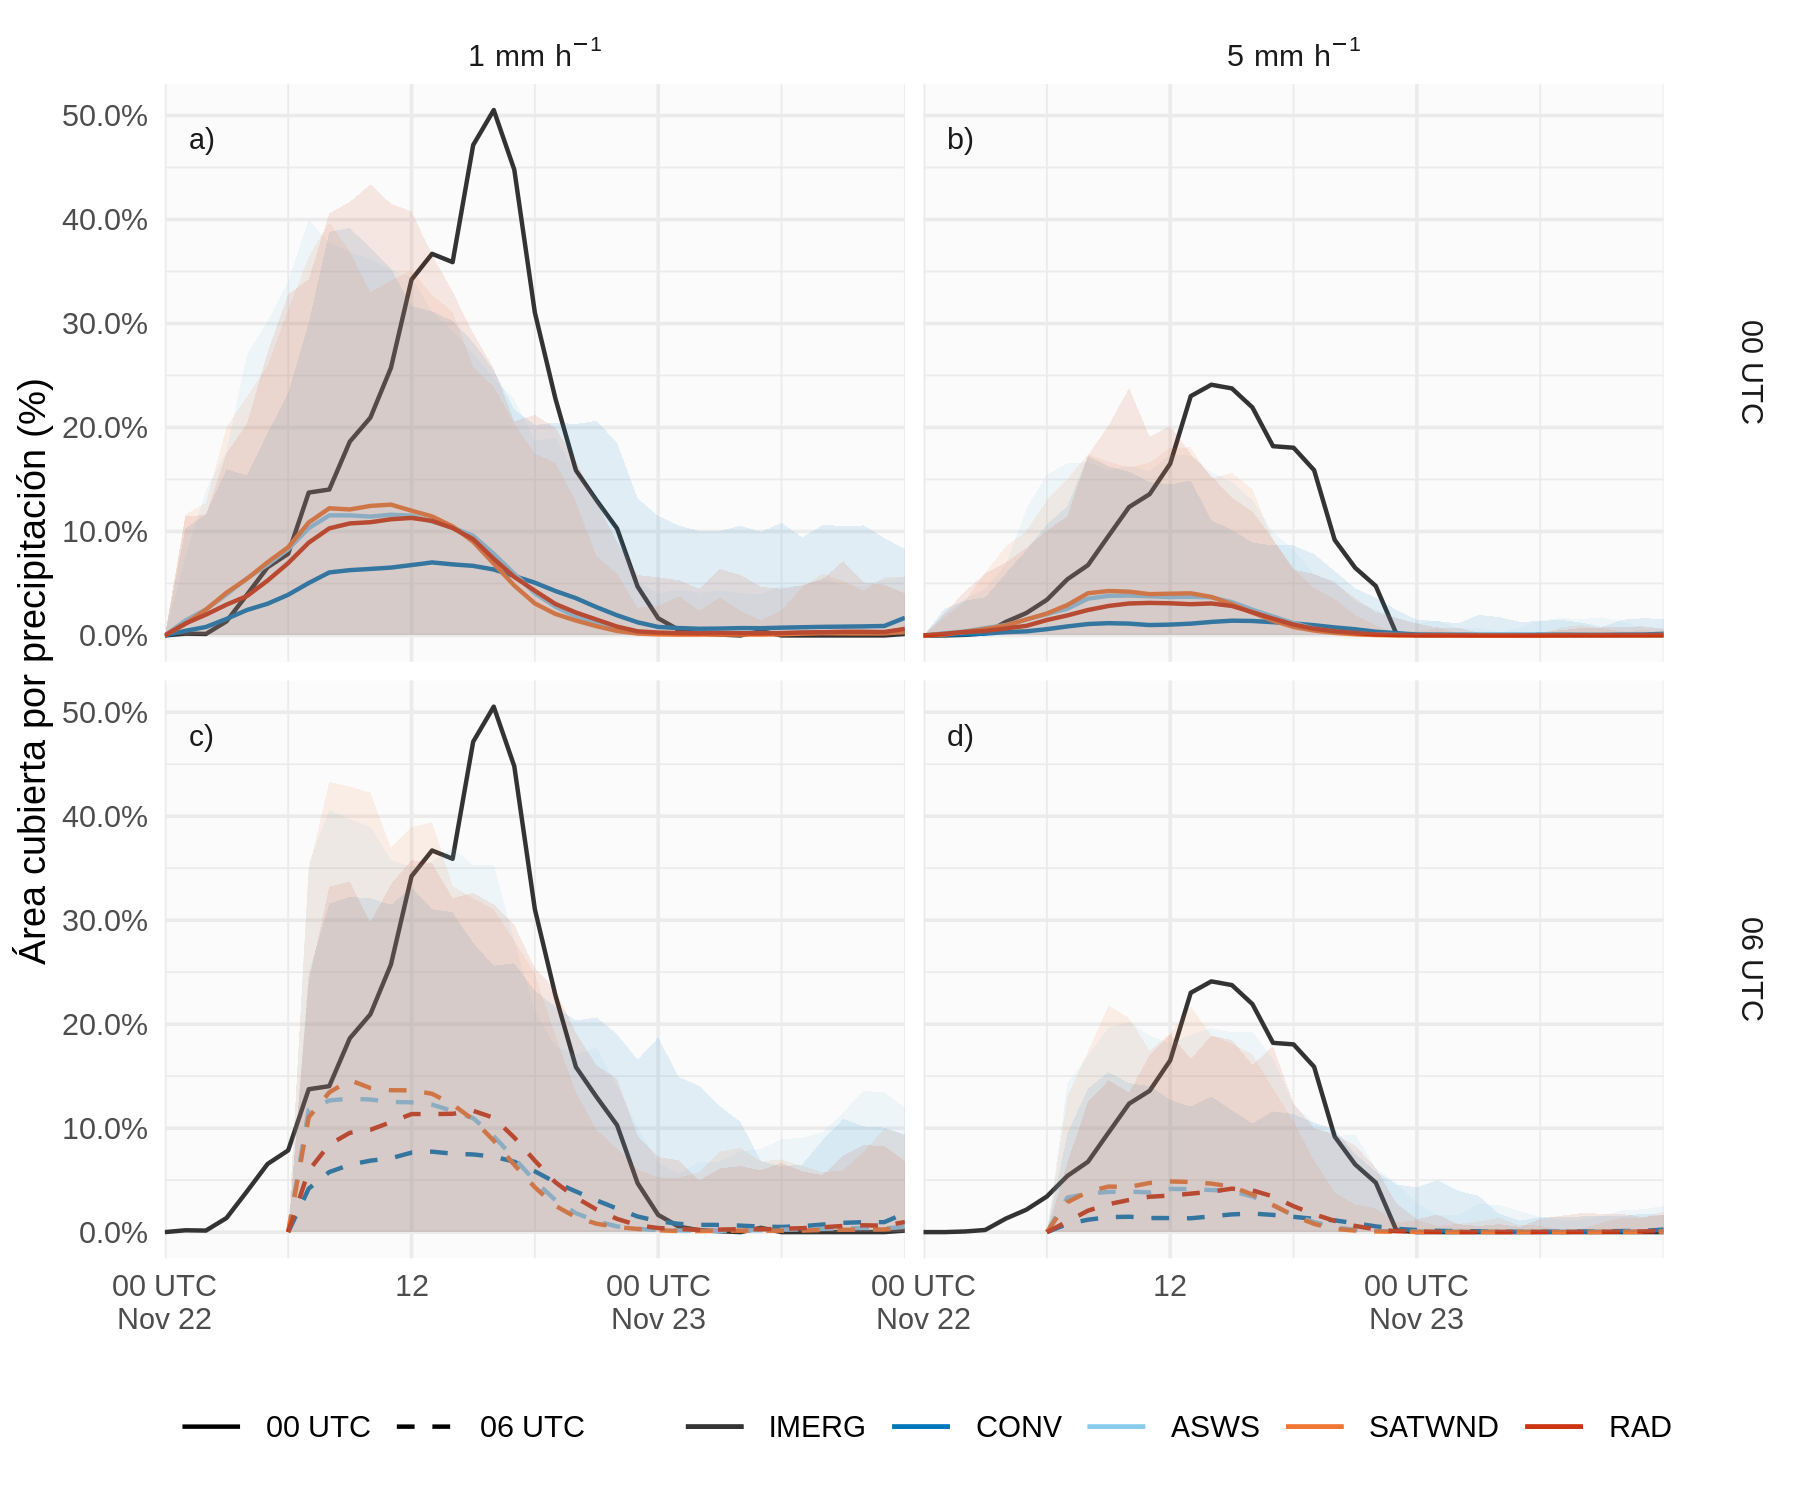
\includegraphics{thesis_files/figure-latex/area-1} \caption{Porcentaje de área cubierta por precipitación superior a \(1 mmh^{-1}\) (a y c) y \(5 mmh^{-1}\) (b y d) a lo largo del tiempo para los pronósticos inicializados a partir de los experimentos CONV (línea azul), AWS (línea celeste), SATWND (línea naranja) y RAD (línea roja) a las 00 UTC (línea sólida) y 06 UTC (linea punteada) del 22 de noviembre. En sombreado y para cada experimento se muestra el área máxima y mínima estimada por el ensamble de pronósticos. En línea continua negra se muetra la estimación de IMERG.}\label{fig:area}
\end{figure}
Por otro lado, se generaron diagramas de confiabilidad usando probabilidades pronósticadas de 0, 20, 40, 60, 80 y 100\% calculadas sobre el ensamble para los pronósticos inicializados a las 00 UTC (Figuras \ref{fig:reliability-1}) y 06 UTC (Figuras \ref{fig:reliability-2}) utilizando percentiles de precipitación calculados sobre todo el periodo pronosticado (Tabla \ref{tab:quantiles}). En un diagrama de confiabilidad, la línea diagonal representa un pronóstico totalmente confiable. Por el contrario, pronósticos por debajo de la diagonal sobreestiman la ocurrencia del evento observado y pronósticos por encima de la diagonal, subestiman la ocurrencia del evento.

Los pronósticos inicializados a las 00 UTC muestran curvas de confiabilidad con tendencia positiva, por lo que son considerados confiables. Sin embargo, para probabilidades de precipitación hasta 60\%, los pronósticos subestiman la ocurrencia de precipitación. Esta subestimación aumenta a medida que aumenta el percentil (Figuras \ref{fig:reliability-1}c-d), lo que indica que los pronósticos subestiman la ocurrencia de precipitación muy intensa. En probabilidades del ensamble superiores al 60\%, los pronósticos sobreestiman la ocurrencia de precipitación cuando se observan los primeros percentiles (umbrales bajos) o son incapaces de producir estos valores de probabilidad cuando se observan umbrales altos de precipitación. Esto se ve muy claramente en los gráficos de frecuencia relativa de eventos que acompañan cada diagrama de confiabilidad, donde la frecuencia de eventos con probabilidades por encima de 60\% es baja o nula.

Los pronósticos inicializados a las 06 UTC muestran tendencias similares, sin embargo es notorio como los umbrales de precipitación asociados a cada percentil, que se muestran en la Tabla \ref{tab:quantiles}, aumentan considerablemente respecto de los pronósticos de las 00 UTC. Es posible que las condiciones iniciales que incluyen nuevas observaciones en conjunto con condiciones de borde actualizadas de GFSF favorezcan un aumento en el desarrollo de la precipitación.

En líneas generales todos los experimentos muestran un comportamiento similar con muy pequeñas diferencias principalmente en el percentil 0.95. Para algunas probabilidades pronósticadas el experimento CONV se observa más cercano a la diagonal, es decir, es más confiable. Sin embargo esto ocurre solo para umbrales pequeños de precipitación ya que subestima umbrales más altos (Figura \ref{fig:fssfcst}) como así tambien, el área cubierta por precipitación (Figura \ref{fig:area})




\begin{figure}

{\centering 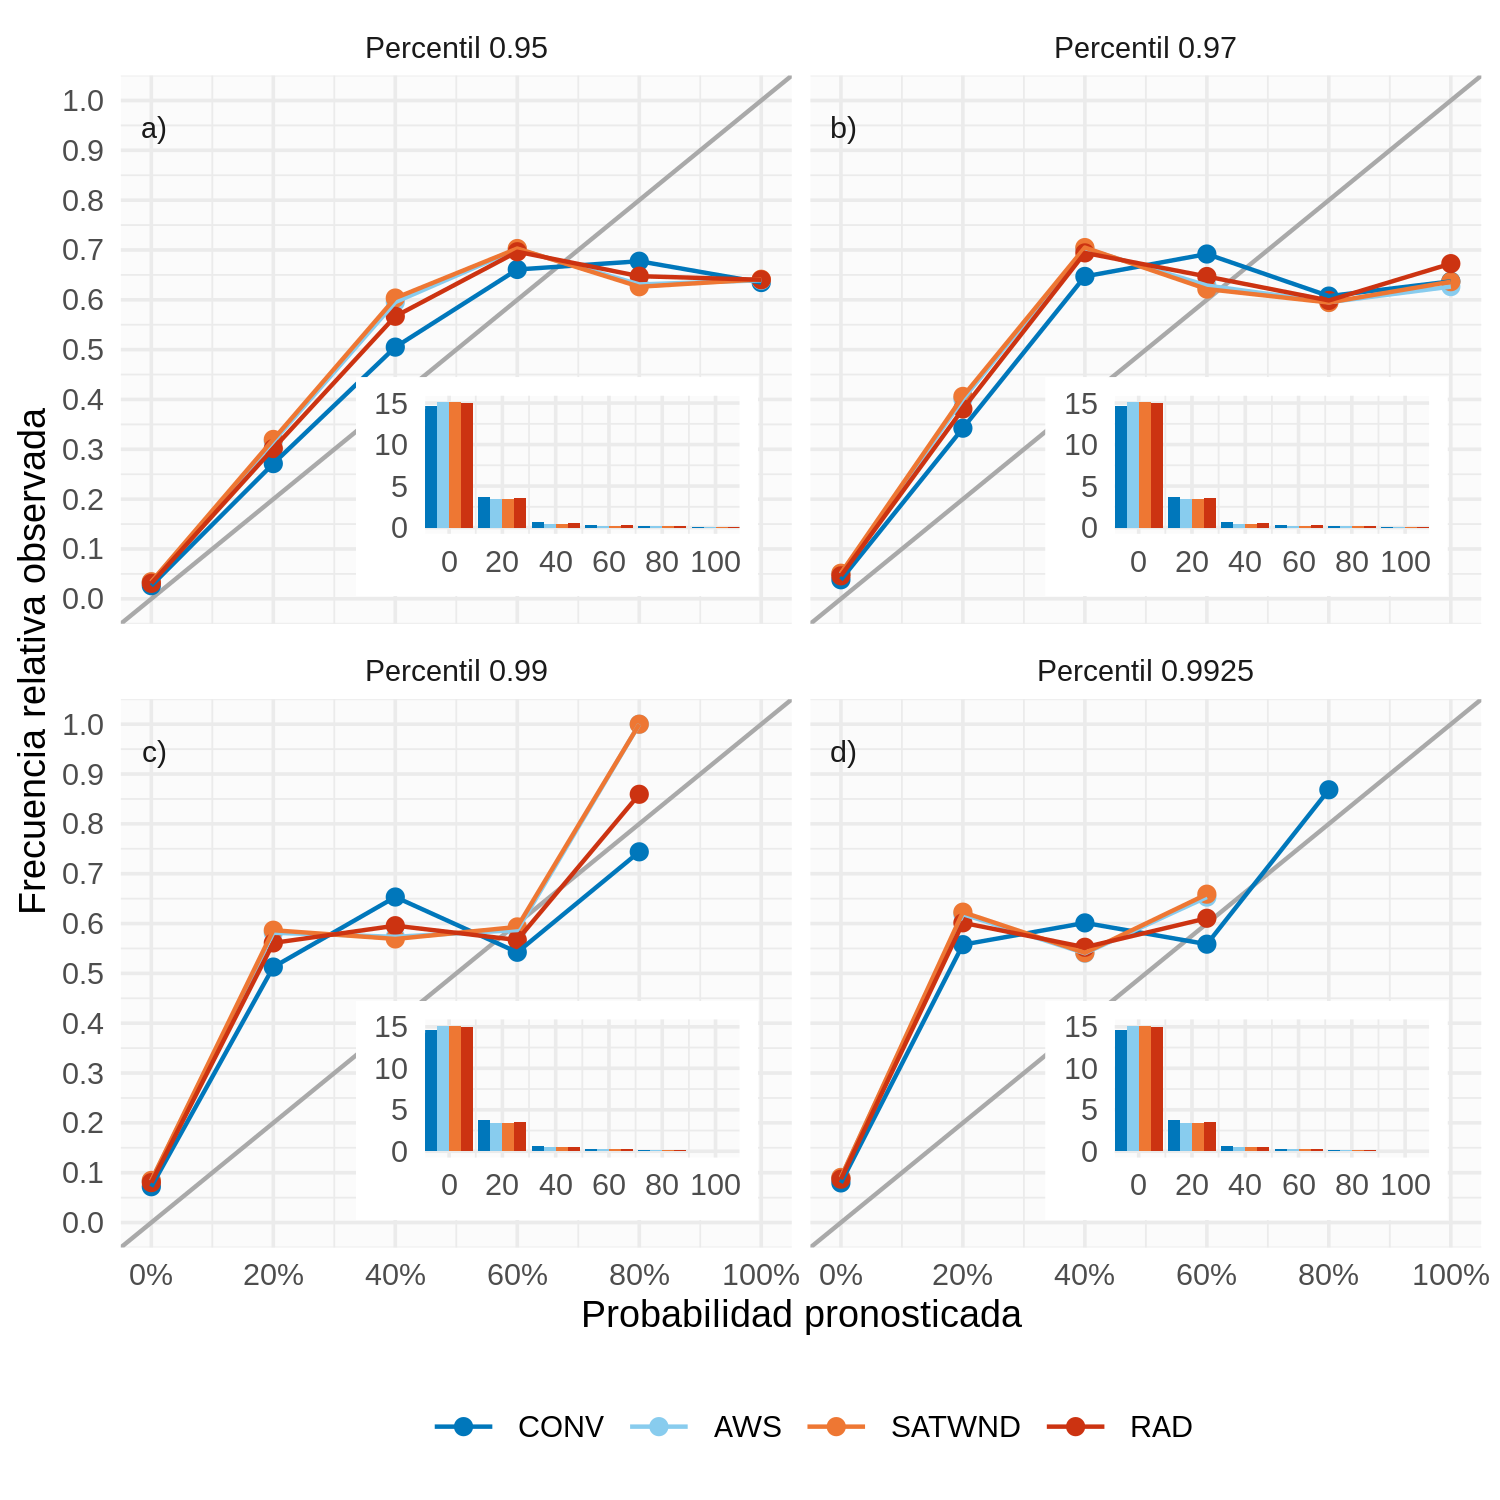
\includegraphics{thesis_files/figure-latex/reliability-1} 

}

\caption{Diagrama de confiabilidad calculado sobre el pronóstico inicializado a las 00UTC para probabilidades de 0, 20, 40, 60, 80 y 100\% de ocurrencia de precipitación acumulada en 3 horas mayor al percentil a) 0.95, b) 0.97, c) 0.99 y d) 0.9925. Los gráficos secundarios dentro de cada diagrama muestran la frecuencia relativa de eventos (x 100.000) asociada a cada intervalo de probabilidad para cada percentil.}\label{fig:reliability-1}
\end{figure}
\begin{figure}

{\centering 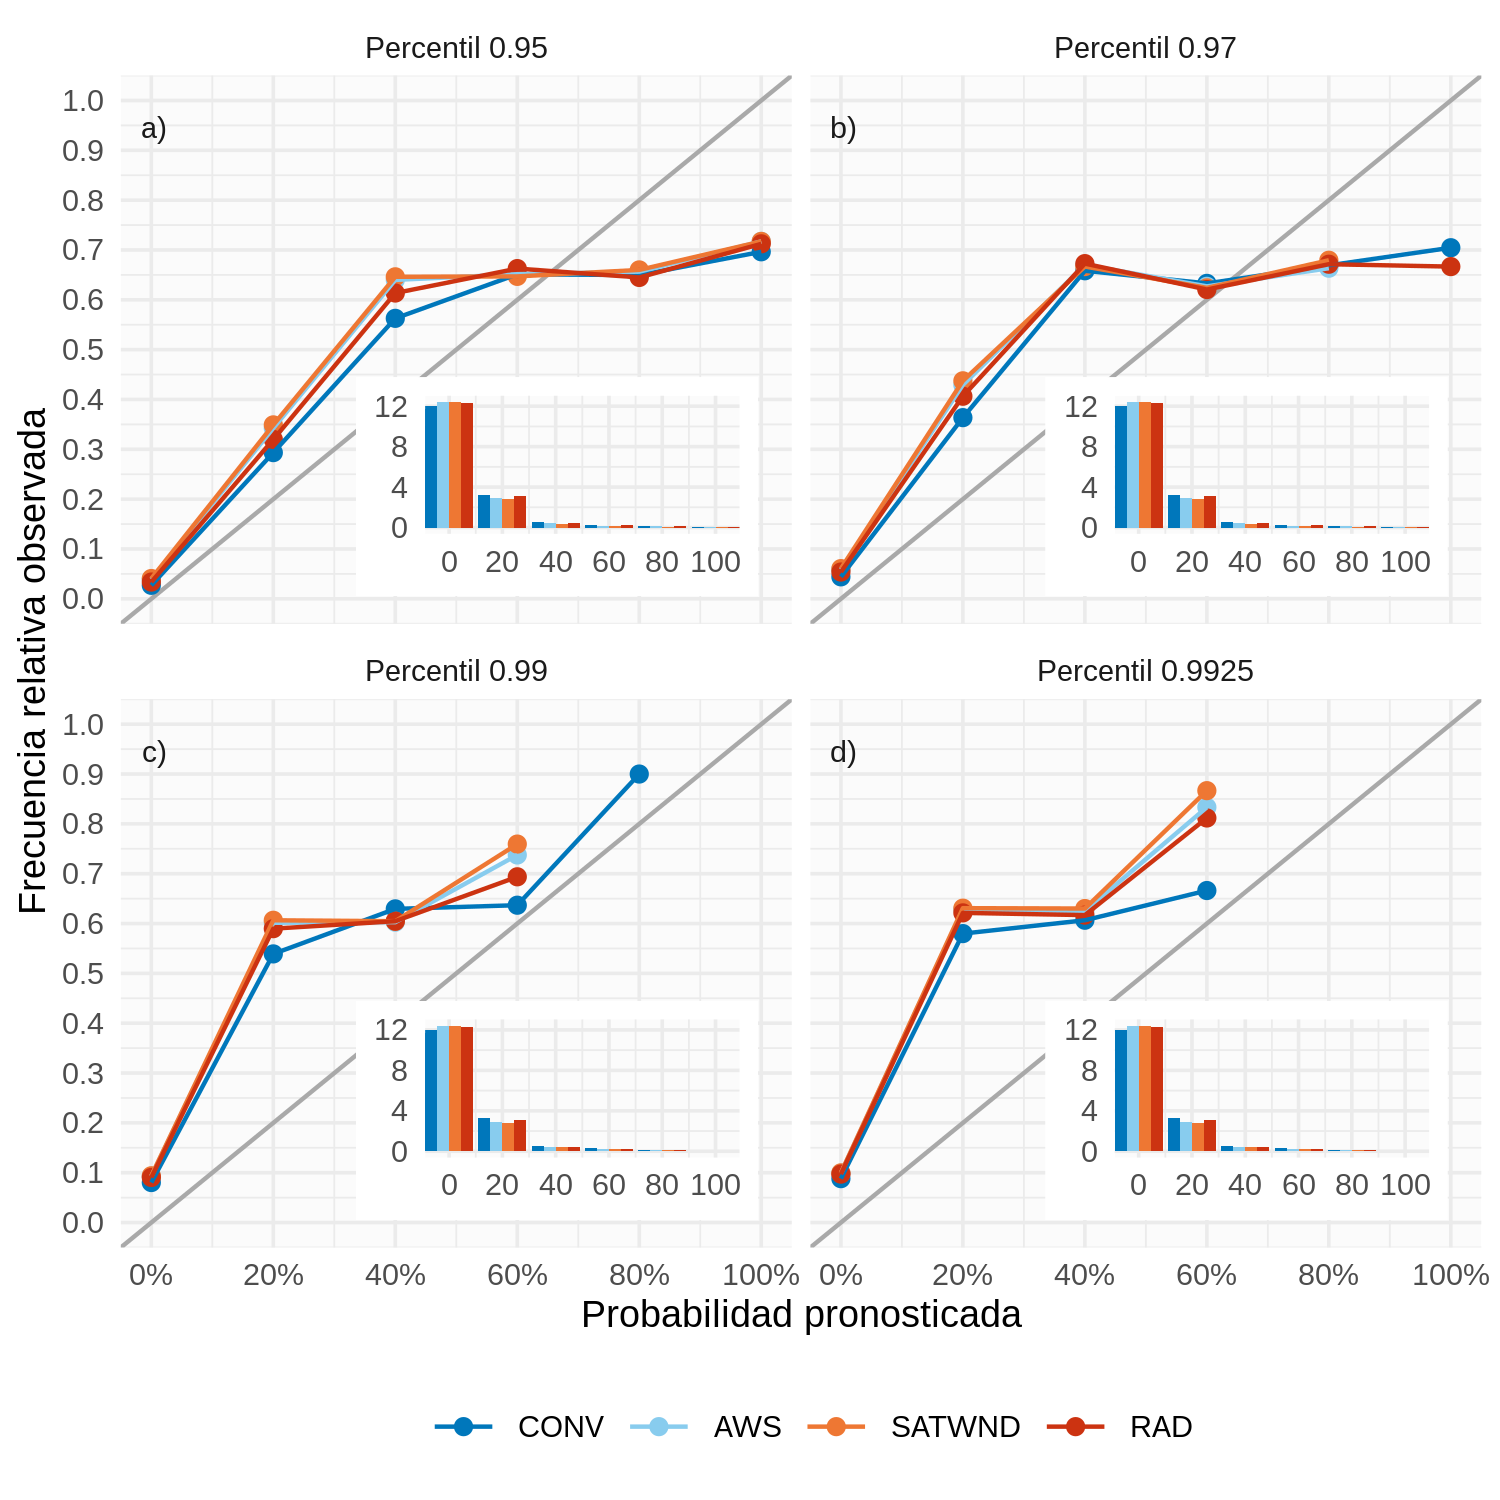
\includegraphics{thesis_files/figure-latex/reliability-2} 

}

\caption{Cómo en la Figura \ref{fig:reliability-1} pero pera el pronóstico inicializado a las 06 UTC}\label{fig:reliability-2}
\end{figure}
\begin{table}

\caption{\label{tab:quantiles}Valor de la precipitación acumulada en 3 hs asociada a distintos percentiles calculados para cada inicialización de pronóstico y cada experimento.}
\centering
\fontsize{10}{12}\selectfont
\begin{tabular}[t]{llrrrr}
\toprule
Experimento & Pronóstico & 0.95 & 0.97 & 0.99 & 0.9925\\
\midrule
CONV &  & 2.14 & 4.59 & 14.94 & 19.10\\
\cmidrule{1-1}
\cmidrule{3-6}
AWS &  & 3.50 & 7.30 & 21.68 & 26.70\\
\cmidrule{1-1}
\cmidrule{3-6}
SATWND &  & 3.66 & 7.62 & 22.31 & 27.42\\
\cmidrule{1-1}
\cmidrule{3-6}
RAD & \multirow{-4}{*}{\raggedright\arraybackslash 00 UTC} & 3.03 & 6.32 & 19.41 & 24.26\\
\cmidrule{1-6}
CONV &  & 2.88 & 5.86 & 18.39 & 23.20\\
\cmidrule{1-1}
\cmidrule{3-6}
AWS &  & 4.82 & 9.45 & 26.52 & 32.30\\
\cmidrule{1-1}
\cmidrule{3-6}
SATWND &  & 5.11 & 9.99 & 27.36 & 33.19\\
\cmidrule{1-1}
\cmidrule{3-6}
RAD & \multirow{-4}{*}{\raggedright\arraybackslash 06 UTC} & 3.88 & 8.07 & 24.72 & 30.56\\
\bottomrule
\end{tabular}
\end{table}
Finalmente las Figuras \ref{fig:prob} muestran la probabilidad de ocurrencia de precipitaición acumulada en en 36 hs para los pronósticos inicializados a las 00 UTC y 30 hs para los pronósticos inicializados a las 06 UTC; para distintos umbrales de precipitación.

Los campos de probabilidad de precipitación mayor a 10 mm (Figuras \ref{fig:prob}a-h), muestra que la precipitación se genera más hacia el norte y oeste de lo observado (línea negra). Esto podría indicar que los pronósticos tienen un demora al generar precipitación al comienzo del periodo. Esto también se observa en la Figura \ref{fig:fssfcst} donde se ve que los valores de FSS van aumentando en las primeras horas de pronóstico, es decir, la precipitación se acerca lo observado tanto en magnitud como en localización. Sin embargo, es notoria la mejora que se produce en los experimentos que se generaron a partir de condiciones iniciales con asimilación de EMA y vientos derivados de satélite respecto de CONV. Los pronósticos RAD si bien son mejores que CONV, subestiman la intensidad de la precipitación en mayor medida que SATWND.

Las Figuras \ref{fig:prob}i-p muestran los campos de probabilidad de precipitación superior a 50 mm donde se puede apreciar una vez más como los pronósticos subestiman la precipitación, en particular para los umbrales más altos. Al igual que para el umbral de 10 mm, es interesante notar la mejora que se produce entre las inicializaciones. 06 UTC logra representar mucho mejor la distribución de precipitación en el dominio que los pronósticos de las 00 UTC. Por ejemplo, el pronóstico SATWND de las 06 UTC (Figura \ref{fig:prob}o) captura casi la totalidad del área de precipitación observada, aunque solo en un 10\% de los miembros del ensamble.


\begin{figure}

{\centering 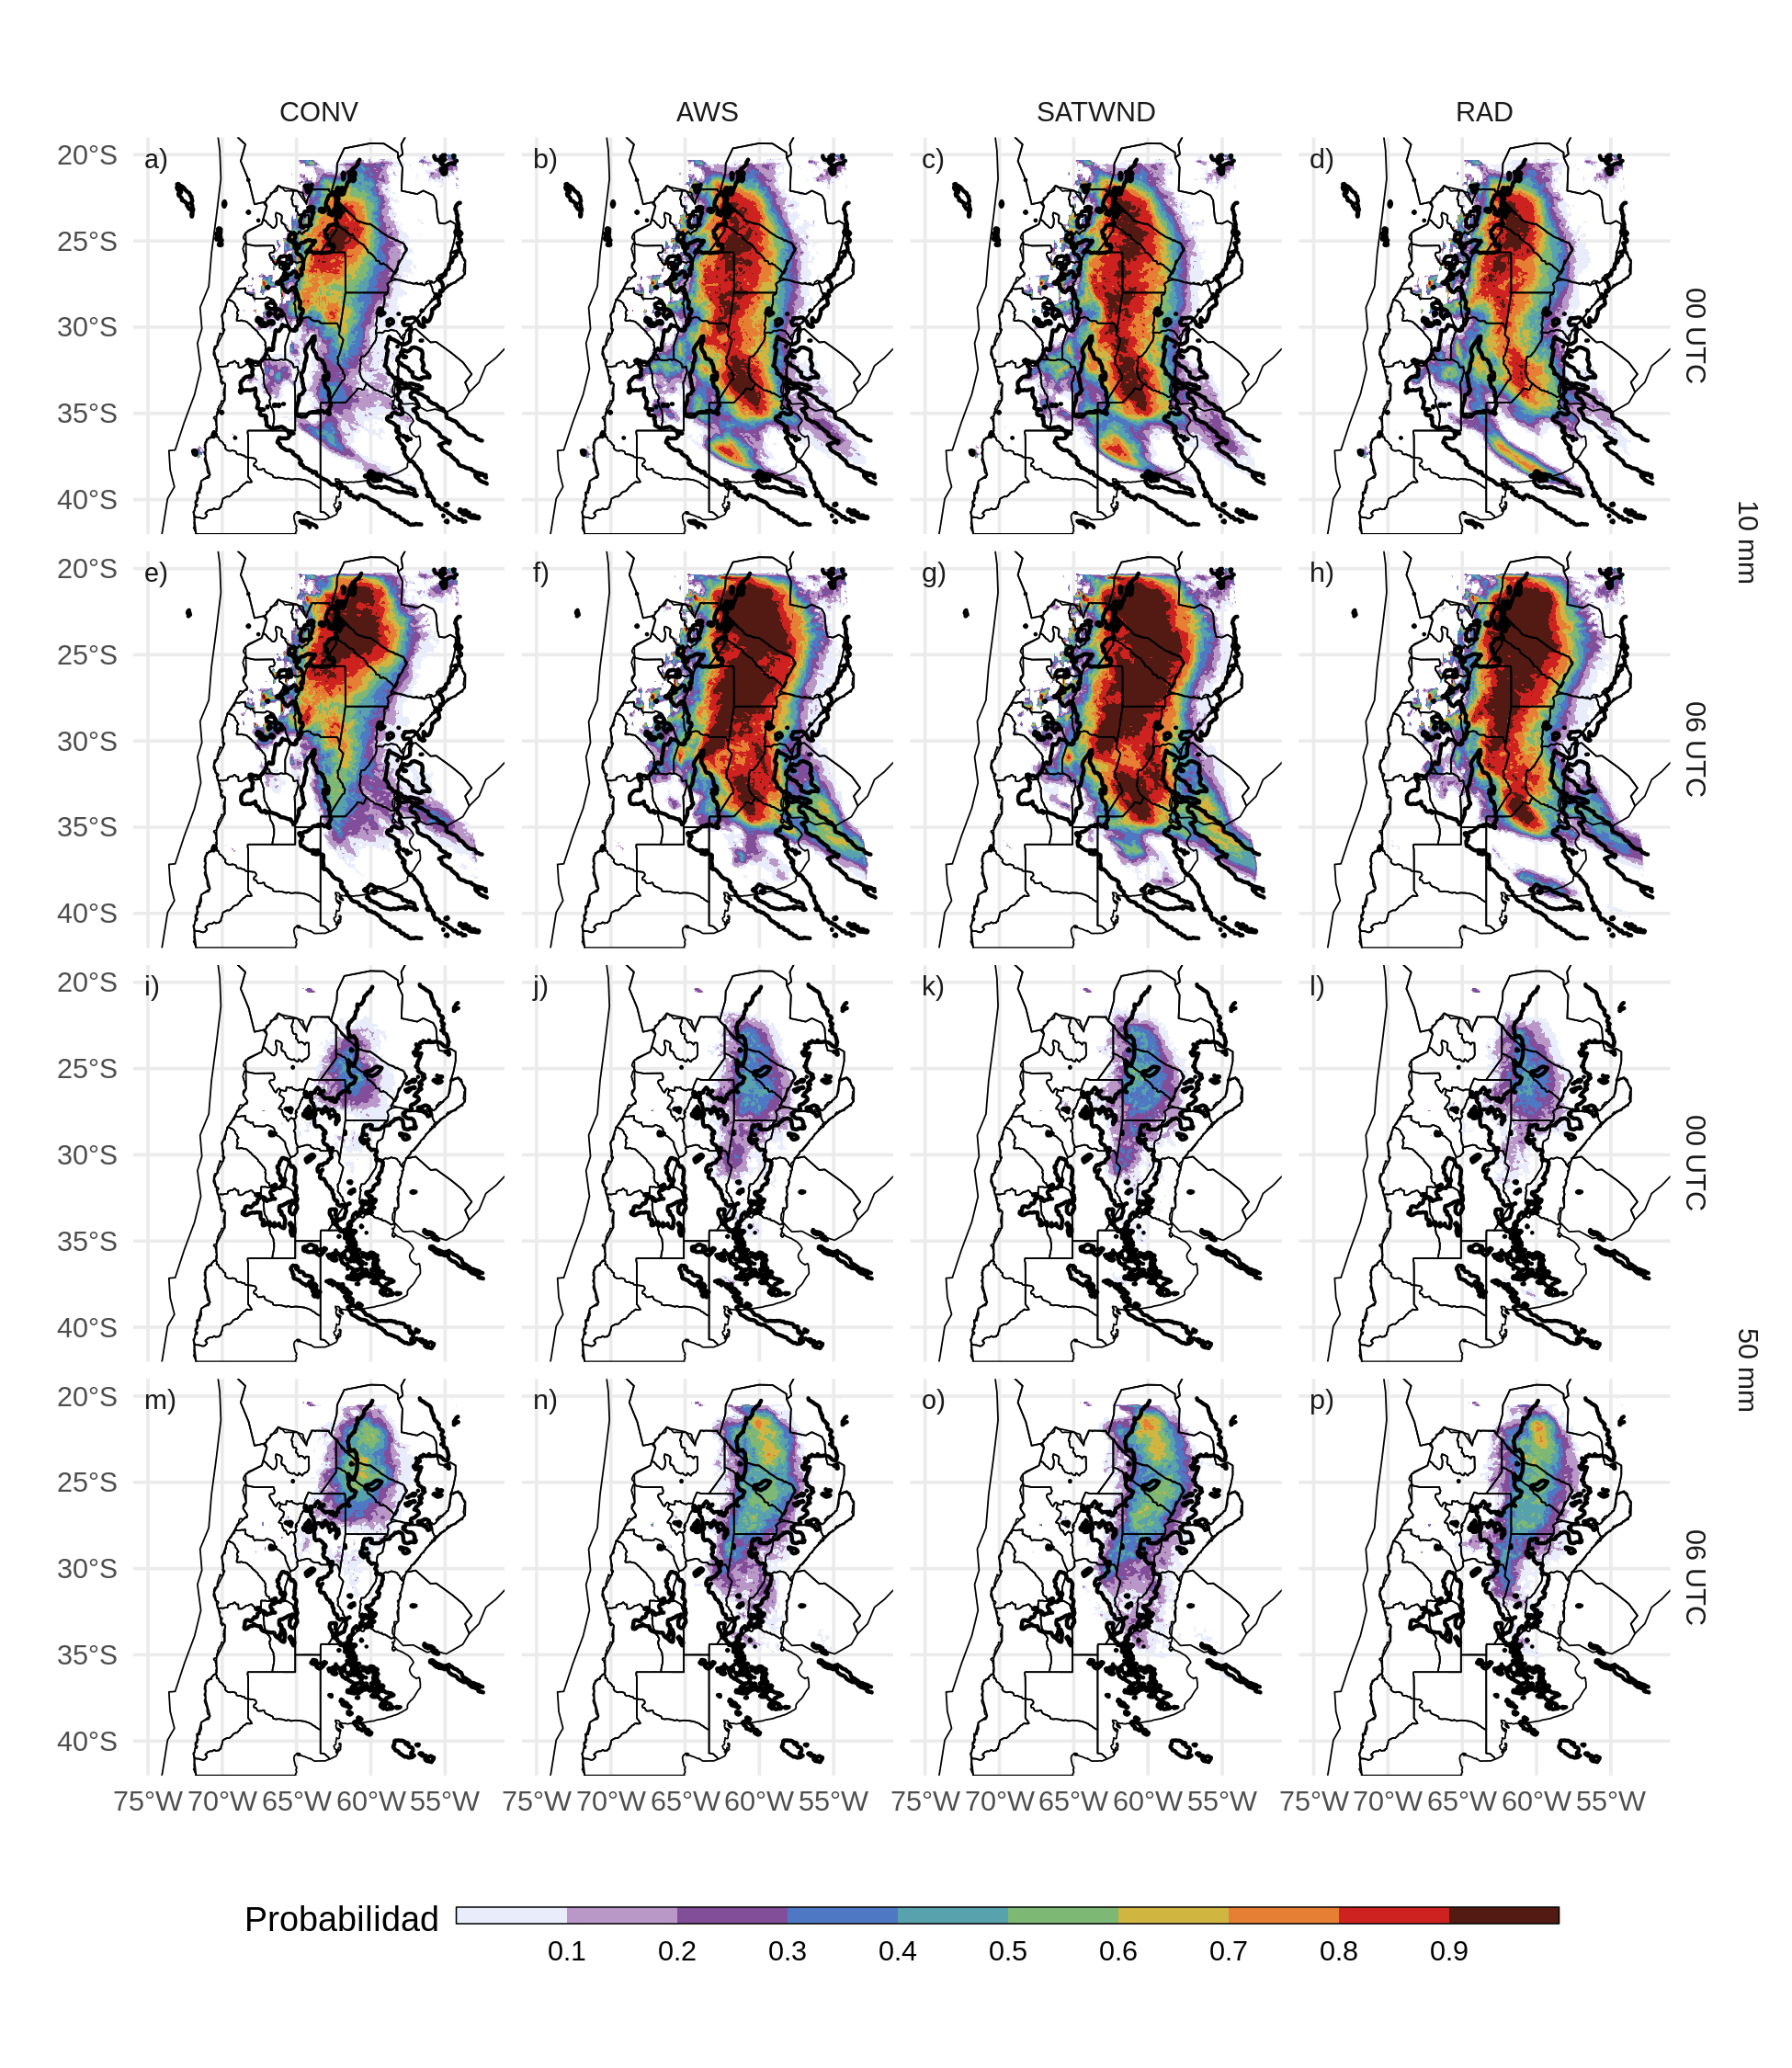
\includegraphics{thesis_files/figure-latex/prob-1} 

}

\caption{Probabilidad de ocurrencia de precipitación acumulada en 36 y 30 hs superior a 10 mm (fila 1 y 2) y 50 mm (fila 3 y 4) para los pronósticos inicializados a las 00 y 06 UTC respectivamente.}\label{fig:prob}
\end{figure}
\hypertarget{anuxe1lisis-y-verificaciuxf3n-por-parametrizaciones}{%
\subsection{Análisis y verificación por parametrizaciones}\label{anuxe1lisis-y-verificaciuxf3n-por-parametrizaciones}}

En esta sección evaluamos los pronósticos de manera cuantitatva comparándolos con observaciones de EMA, que si bien son asimiladas en los experimentos de análisis, son observaciones independietes para los pronósticos y radiosondeos de la campaña RELAMPAGO.

En primer lugar se calculó el RMSE y BIAS respecto de las observaciones de EMA a lo largo del tiempo para cada pronóstico e inicialización. El BIAS y RMSE de la humedad específica (Figuras \ref{fig:rmse-bias-aut}a y e) al comienzo de los pronósticos es coherente con las condiciones iniciales. Por ejemplo el BIAS seco asociado a CONV es mucho más importante que el los pronósticos inicializados a partir de AWS. También se observan mejoras en la inicialización de las 06 UTC, algo que no era evidente en el análisis de los perfiles verticales promediados espacialmente (Figura \ref{fig:era5-fcst-2}). Los errores asociados a la temperatura (Figuras \ref{fig:rmse-bias-aut}b y f) son muy dependientes del momento del día, con un aumento del RMSE y del BIAS cálido durante las horas nocturnas. Los pronósticos CONV y RAD para la inicialización de las 06 UTC tienen un mejor densempeño en las primeras horas de pronóstico pero luego se degradan más rápidamente que AWS o SATWND.

Mientras que no hay características sobresalientes en los errores del viento zonal, en el viento meridional (Figuras \ref{fig:rmse-bias-aut}d y h), es interesante notar que el RMSE de los pronósticos de las 06 UTC es más bajo que para los pronósticos de las 00 UTC y esta mejora se mantiene por al menos 6 horas. Esto también ocurre en el BIAS aunque en menor medida.


\begin{figure}
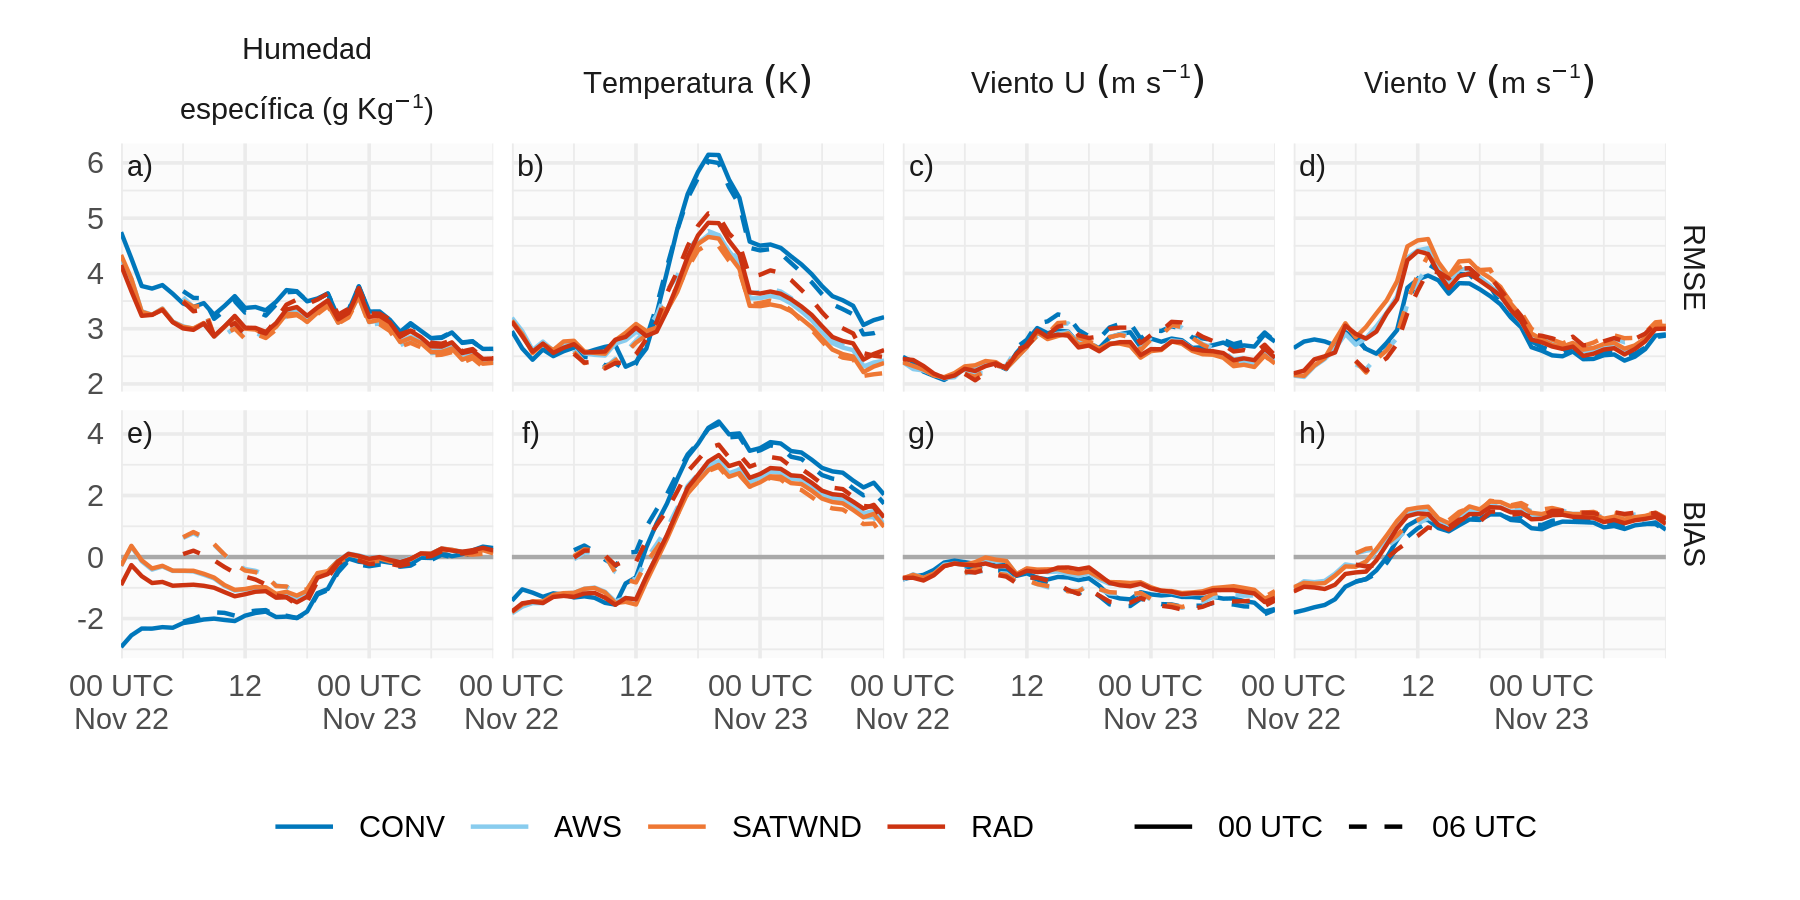
\includegraphics{thesis_files/figure-latex/rmse-bias-aut-1} \caption{RMSE (línea sólida) y Bias (línea discontinua) de a) humedad especifica (\(g\ Kg{^-1}\)), b) temperatura (\(K\)), c) el viento u (\(m\ s^{-1}\)) y d) el viento v (\(m\ s^{-1}\)) calculados comparando los pronósticos de cada experimento con las observaciones de EMA. La línea azul corresponde a CONV, la línea celeste a AWS, SATWND se representa con una línea naranja y RAD con una línea roja.}\label{fig:rmse-bias-aut}
\end{figure}
La Figura \ref{fig:aut-all} muestra el RMSE y BIAS calculado comparando con las observaciones de EMA sobre los miembros del ensamble que utilizan cada una de las parametrizaciones de capa límite. En este caso no se muestran las dos inicializaciones por separado ya que ambos pronósticos presentan tendencias muy similares.

Si bien sería deseable encontrar una parametrización de capa límite que represente correctamente todas las variables de interés, estudios previos (por ejemplo Ruiz et al. (2010) y Dillon et al. (2021)) mostraron que distintas parametrizaciones logran representar correctamente algunas variables pero no todas y que esto puede ser dependiente del caso de estudio. Para esta situación, la parametrización MYJ presenta un menor RMSE y BIAS para las variables termodinámicas (humedad relativa y temperatura) mientras que MYNN2 representa mejor el viento. Sin embargo, a exepción del RMSE del viento, los errores tienen una variabilidad pequeña por lo que la elección de una parametrización u otra podría no tener un impacto importante en la representación de la capa límite. Esto refuerza la necesidad de generar un ensamble multifísica como el utilizado en este trabajo para poder capturar los posibles errores asociados al modelo y la representación de los procesos parametrizados.


\begin{figure}

{\centering 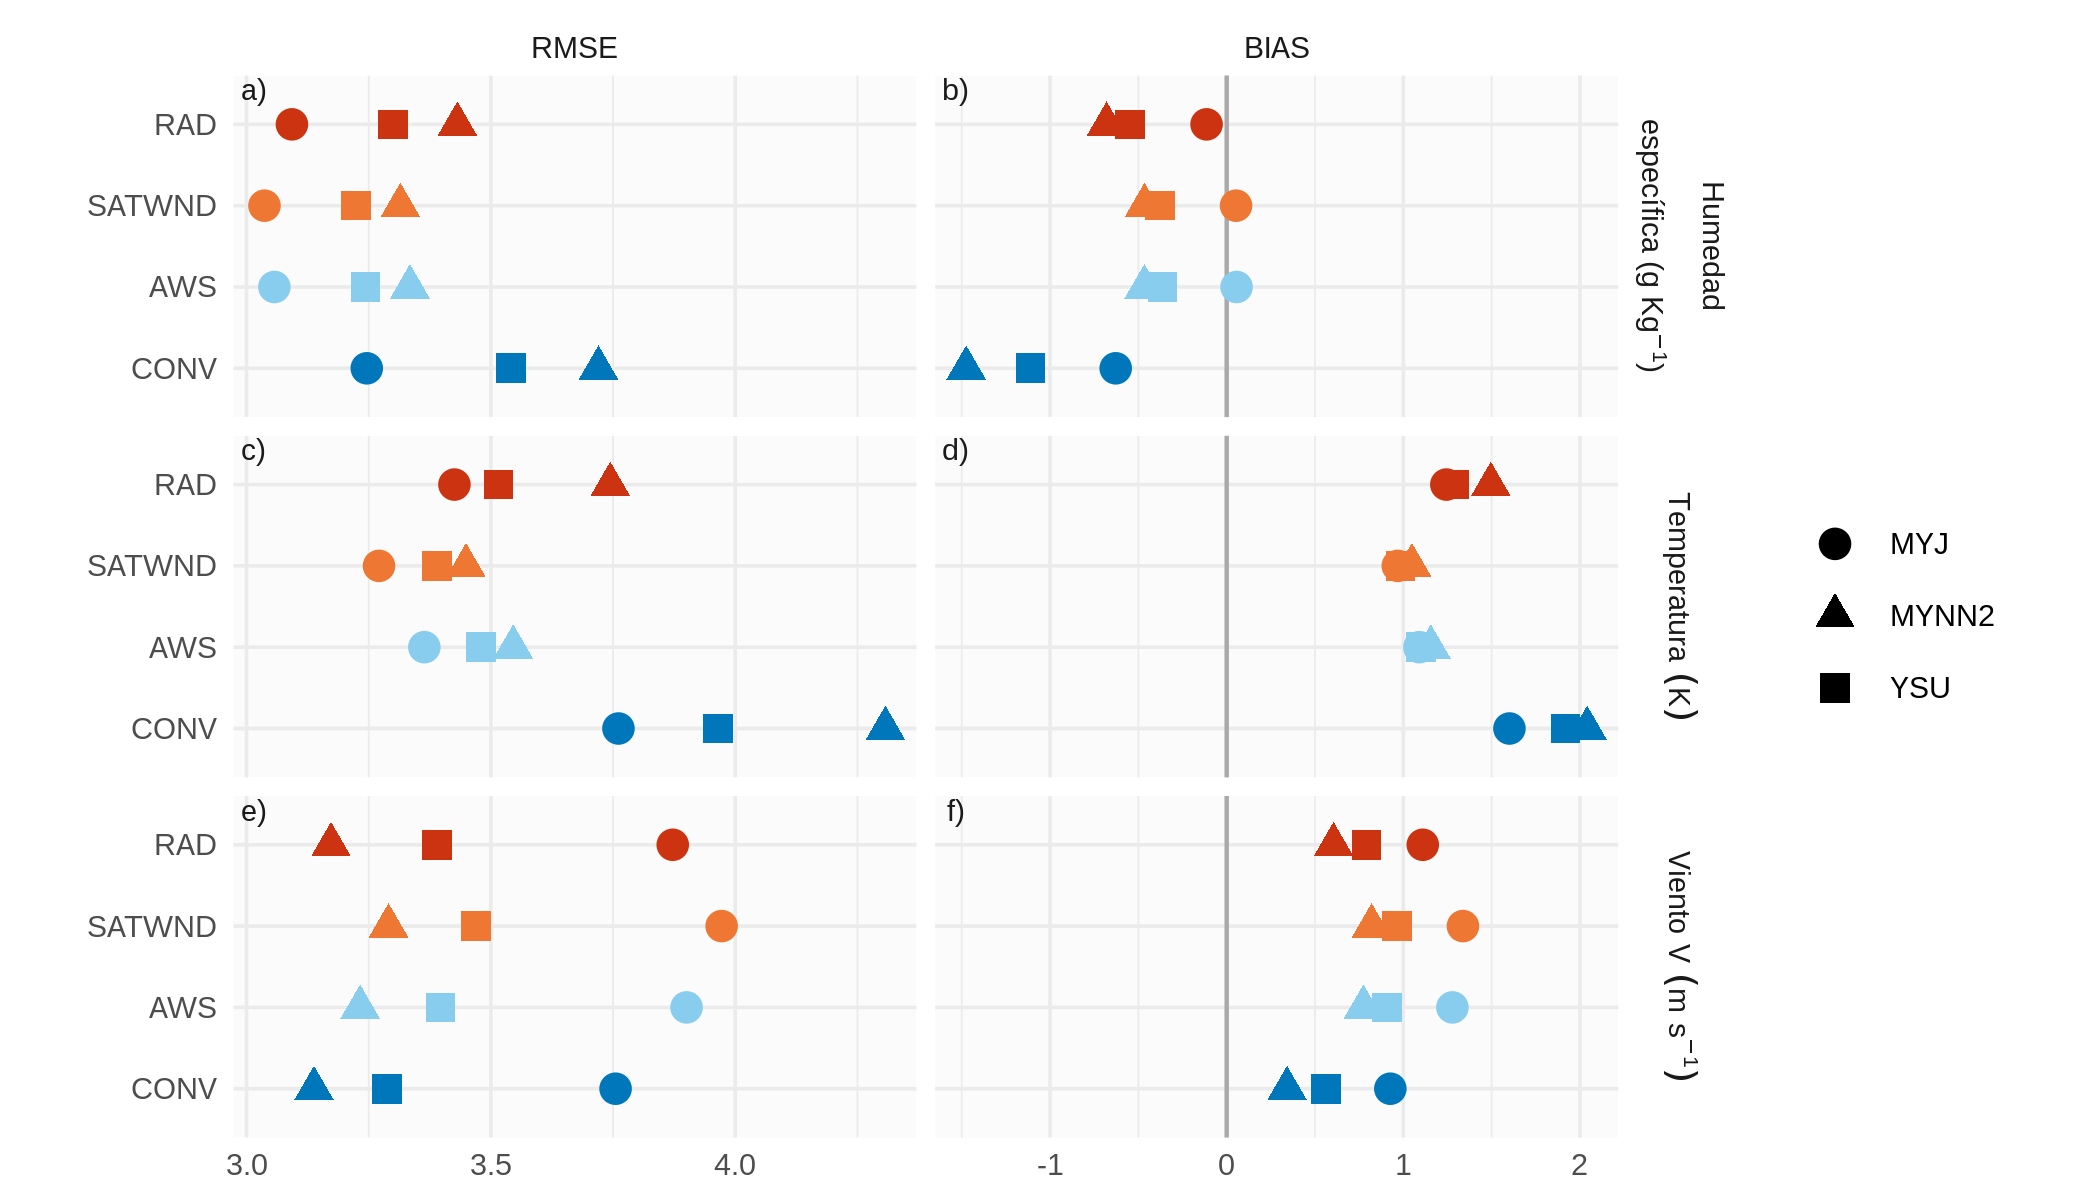
\includegraphics{thesis_files/figure-latex/aut-all-1} 

}

\caption{RMSE y BIAS calculados comparando los pronósticos con observaciones de EMA y promediados sobre los miembros del ensamble que utilizan las parametrizaciones de capa límite MYJ (círculo), MYNN2 (triángulo) e YSU (cuadrado) para todos los pronósticos en conjunto.}\label{fig:aut-all}
\end{figure}
Si se analiza los errores asociados a las parametrizaciones de capa límite a lo largo del periodo pronosticado (Figurs \ref{fig:aut-rad}), en este caso solo para el experimento RAD, la tendencia observada previamente se mantiene. Más importante aún, los errores de ninguna de las parametrizaciones aumenta por sobre el resto, indicando que tienen un comportamiento consistente a lo largo de las 30 y 36 hs de pronóstico.


\begin{figure}

{\centering 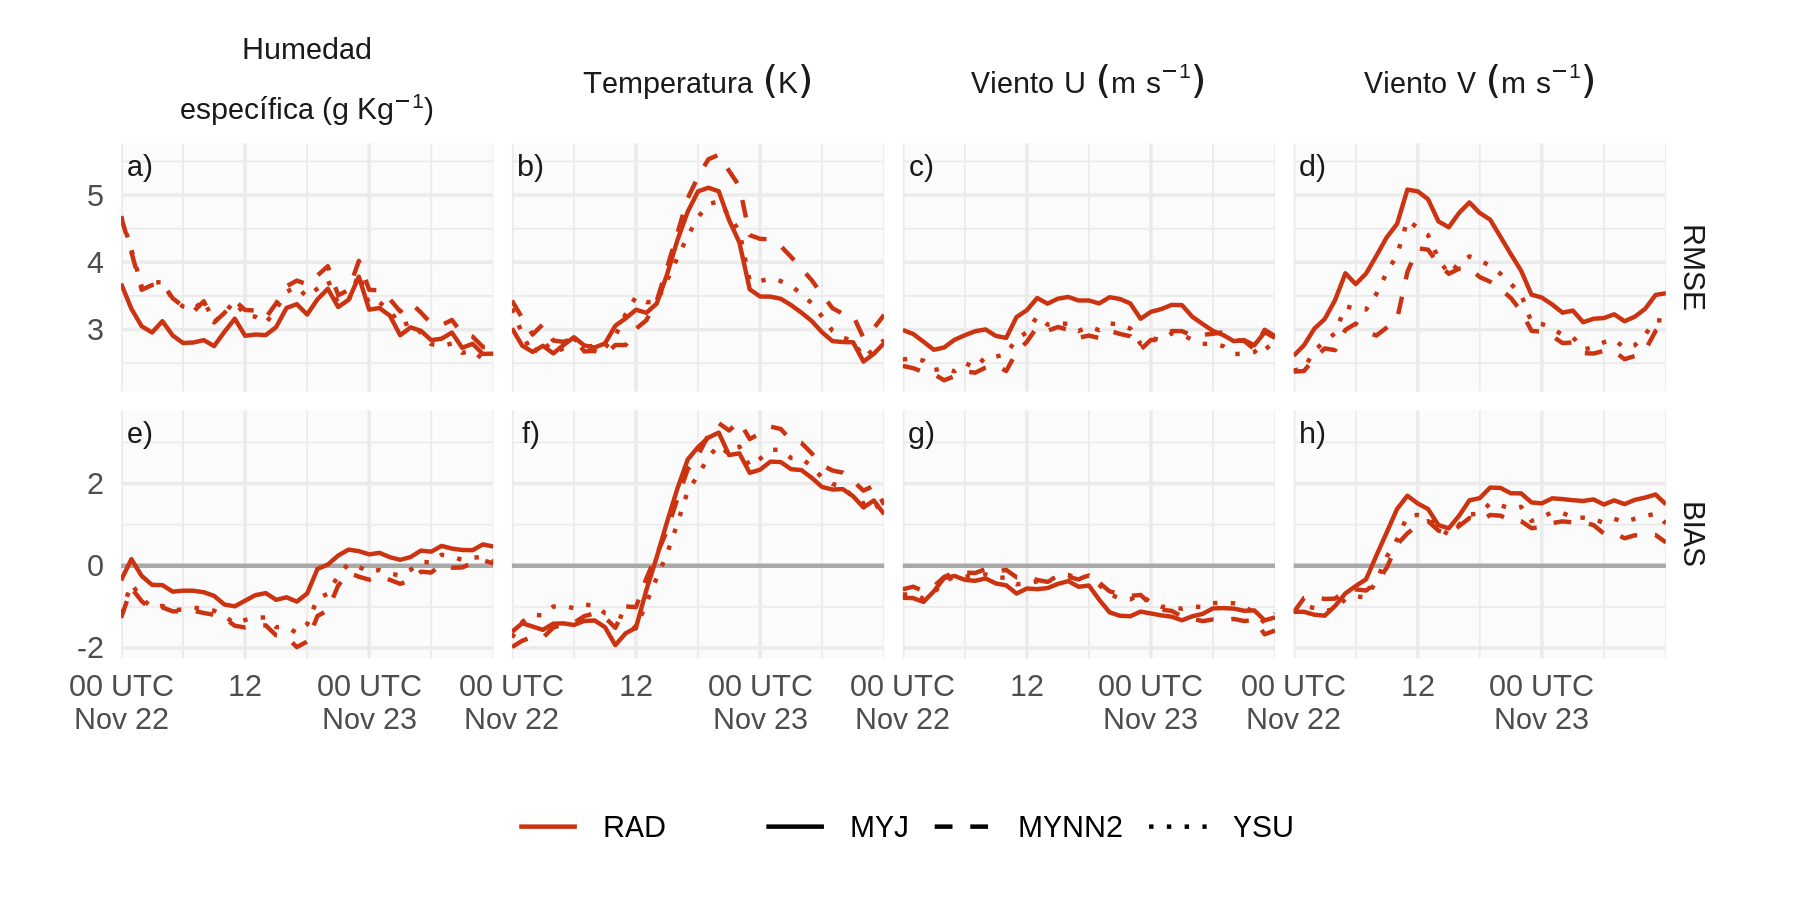
\includegraphics{thesis_files/figure-latex/aut-rad-1} 

}

\caption{RMSE y BIAS calculados comparando los pronósticos con observaciones de EMA y promediados sobre los miembros del ensamble que utilizan las parametrizaciones de capa límite MYJ (línea llena), MYNN2 (línea a rayas) e YSU (línea punteada) para todos los pronósticos en conjunto a lo largo del tiempo de pronóstico.}\label{fig:aut-rad}
\end{figure}
La Figura \ref{fig:soundings-fcst} muestra el RMSE y BIAS calculado comparando los pronósticos con los radiosondeos disponibles durante el periodo pronósticado. En líneas generales no se observan grandes diferencias entre las dos inicializaciones. Si bien los pronósticos de las 06 UTC utilizan condiciones iniciales que incluyen información actualizada del entorno, la mayoría de los radiosondeos fueron lanzados en un área muy pequeña en el centro del dominio (Figura \ref{fig:dominio}b) que podría no haber sido particularmente influenciada por la asimilación de nuevas observaciones.

Es interesante comparar en este punto los errores asociados a los pronósticos con los errores observados en el análisis (Figura \ref{fig:fss}e-h). En general, el rango de valores que toma el RMSE y BIAS para cada variable es similar tanto en los pronósticos como en los análisis, lo que indica que los pronósticos logran representar adecuadamente la situacición en esa región del dominio. Sin embargo, también se observa que los errores son muy parecidos entre experimentos cuando se los compara con los errores de los análisis, por lo que es posible que los errores del modelo y las condiciones de borde, iguales para todos los experimentos, tengan una influencia mayor que las condiciones iniciales de cada pronóstico.

En esta comparación, la característica sobresaliente es la disminución del RMSE y BIAS en niveles bajos en casi todas las variables pero particularmente el viento meridional. El aumento de los errores en los análisis puede atribuirse a la asimilación de observaciones de EMA, que si bien en general producen impactos muy positivos en la representación de la capa límite (por ejemplo, Figura \ref{fig:era5}), en esta región limitada parece generar el efecto contrario. En los pronósticos independiente, sin asimilación continua de estas observacios, los errores en niveles bajos disminuyen a valores cercanos a los observados en los análisis de CONV.


\begin{figure}

{\centering 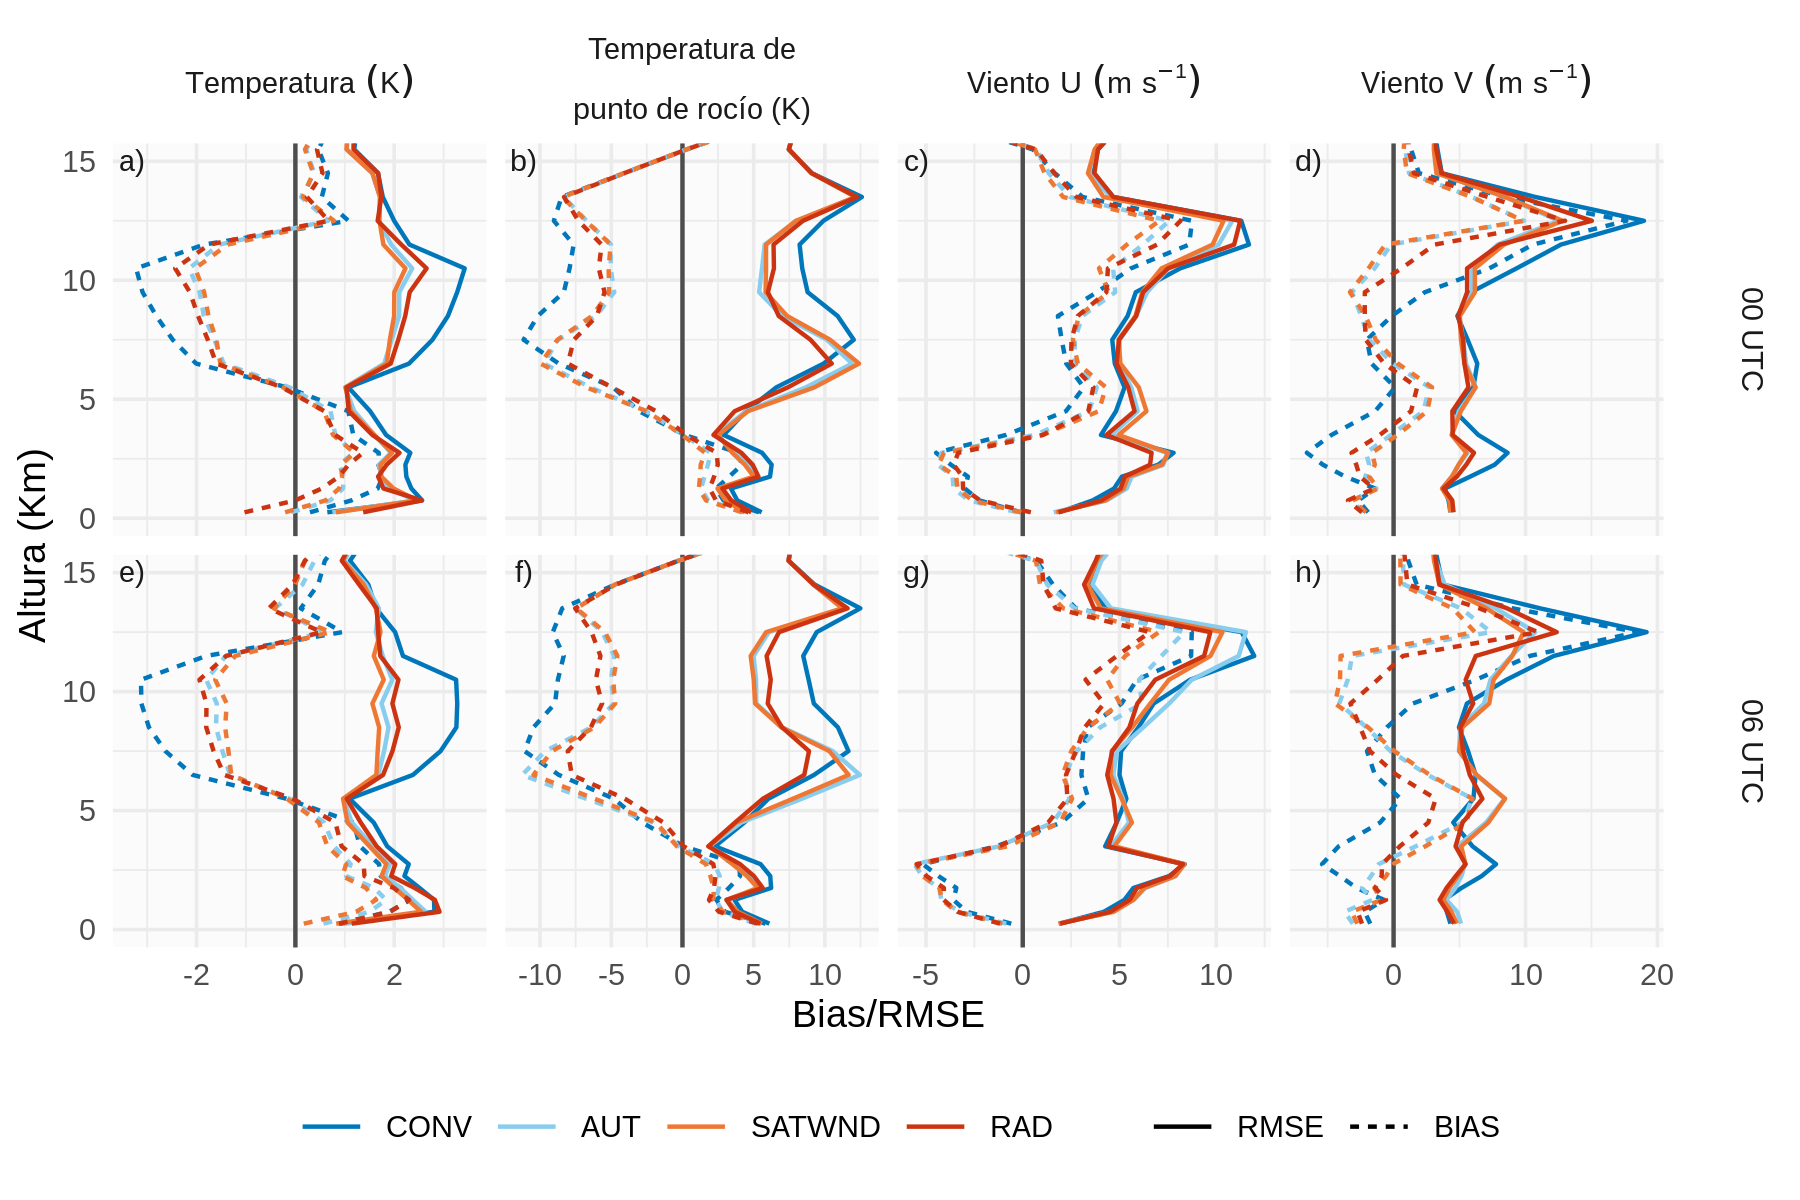
\includegraphics{thesis_files/figure-latex/soundings-fcst-1} 

}

\caption{RMSE (línea sólida) y Bias (línea discontinua) de a) la temperatura (\(K\)), b) la temperatura del punto de rocío (\(K\)), c) el viento u (\(m\ s^{-1}\)) y d) el viento v (\(m\ s^{-1}\)) calculados comparando los pronósticos de cada experimento con los sondeos operativos y de RELAMPAGO. La línea azul corresponde a CONV, la línea celeste a AWS, SATWND se representa con una línea naranja y RAD con una línea roja.}\label{fig:soundings-fcst}
\end{figure}
La Figura \ref{fig:soudings-all} muestra el RMSE y BIAS calculado comparando con los radiosondeos de RELAMPAGO sobre los miembros del ensamble que utilizan cada una de las parametrizaciones de convección. Nuevamente, se muestran las dos inicializaciones en conjunto ya ambos pronósticos presentan tendencias muy similares. Si bien el comportamiento de las parametrizaciones de convección no es tan honomegeo como si sucedía con las de capa límite, es posible identificar algunos patrones. La parametrización BMJ tiene un RMSE menor tanto para la temperatura como para la temperatura de punto de rocio mientras que la parametrización con mejor RMSE es KF.


\begin{figure}

{\centering 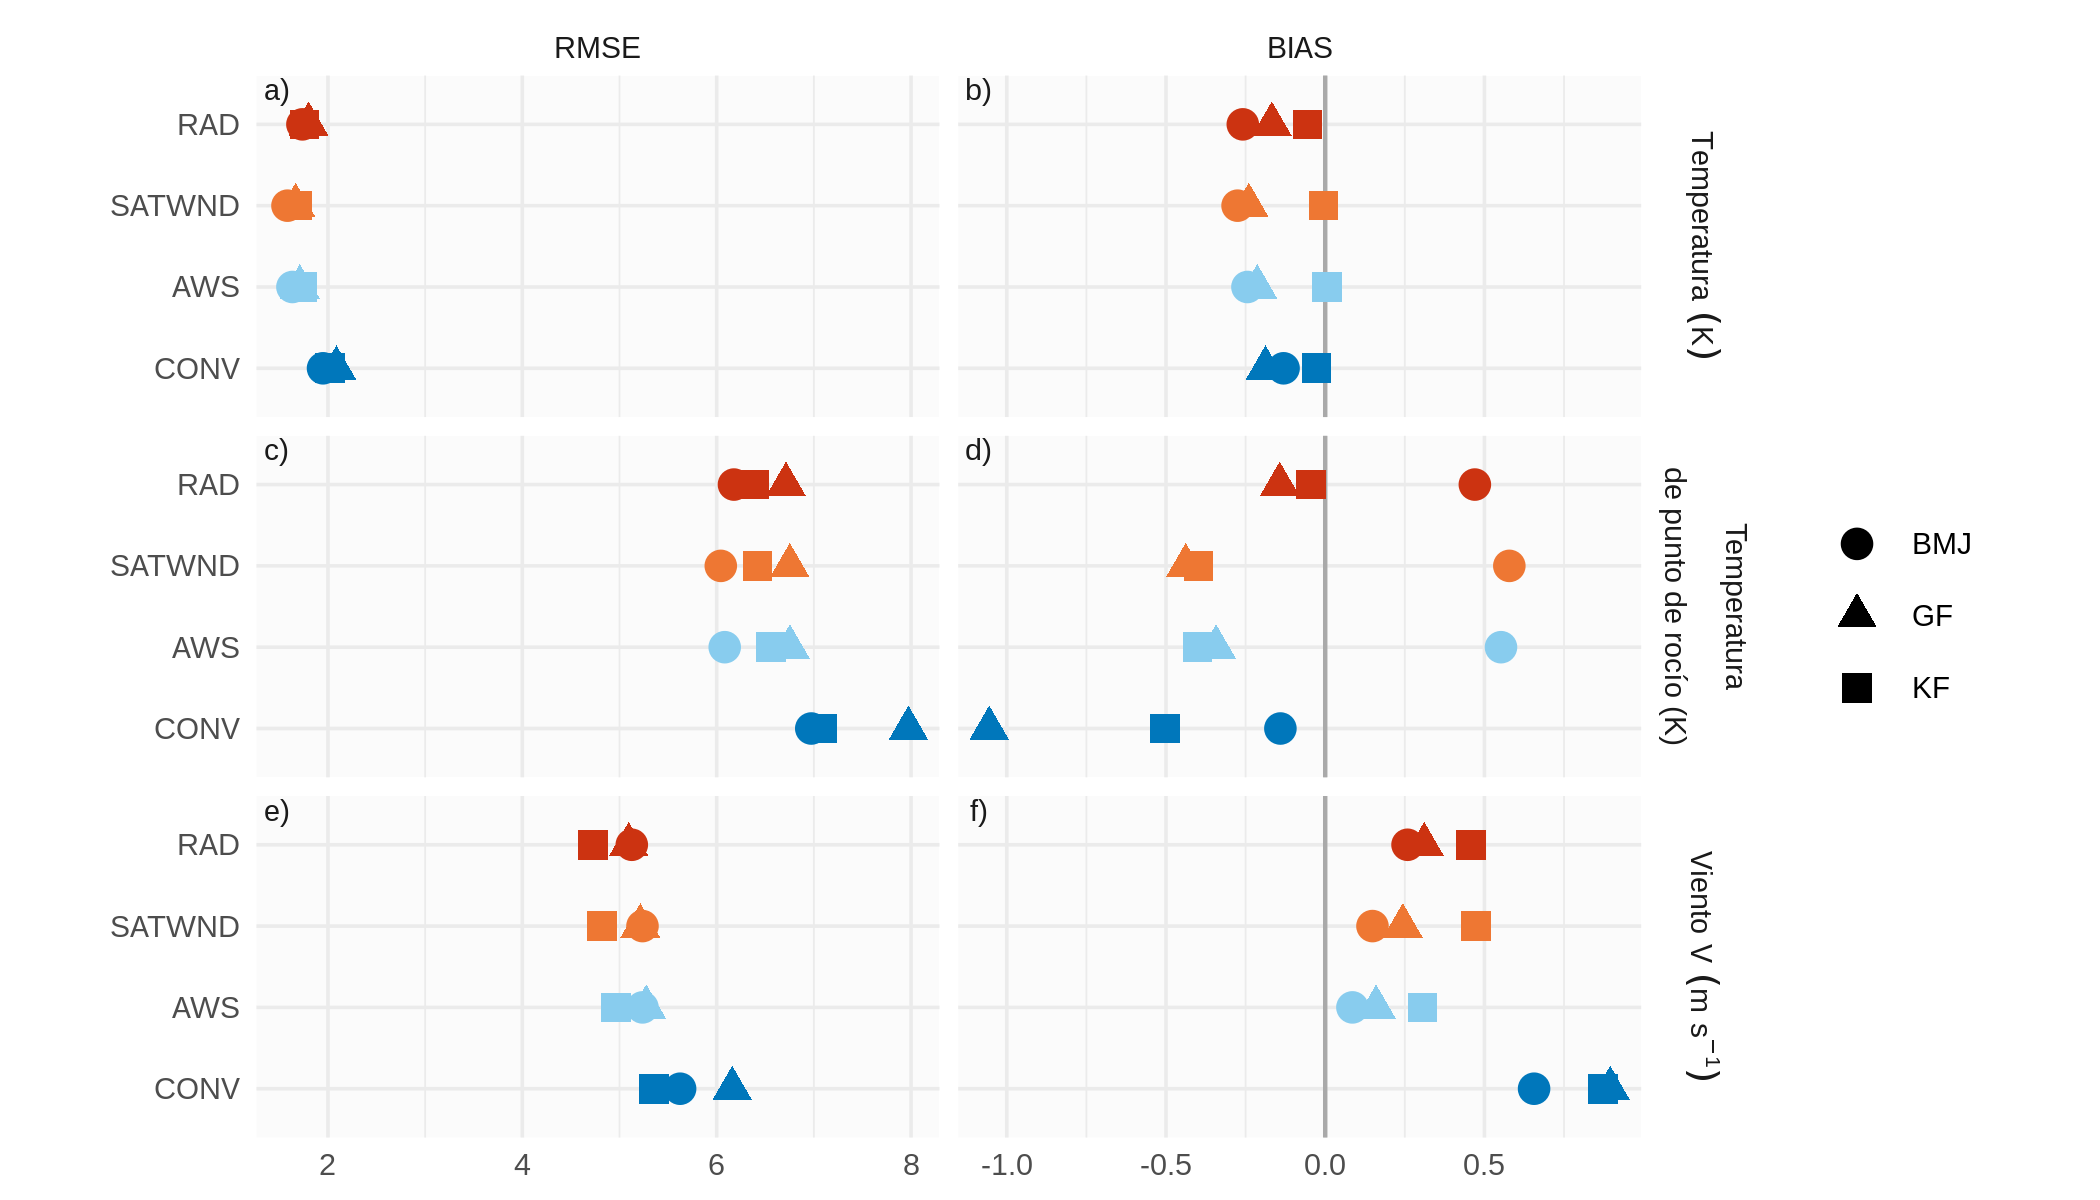
\includegraphics{thesis_files/figure-latex/soudings-all-1} 

}

\caption{RMSE y BIAS calculados comparando los pronósticos con sondeos de RELAMPAGO y promediados sobre los miembros del ensamble que utilizan las parametrizaciones de convección BMJ (círculo), GF (triángulo) e KF (cuadrado) para todos los pronósticos en conjunto.}\label{fig:soudings-all}
\end{figure}
Si analizamos los perfiles verticales de RMSE y BIAS para cada parametrización, calculados solo sobre los pronósticos RAD, podemos ver que BMJ es la parametrización que mejor representa la humedad en niveles medios pero KF representa mejor la mayoría de las variables en niveles bajos.

Si bien no es posible elegir solo una parametrización de convección que mejor represente todas las variables, es interesante observar la buena performance de BMJ al representar estas variables. Sin embargo, Dillon et al. (2021), utilizando una configuración del ensamble multifísica similar a este trabajo, encontraron que esta parametrización era la que peor representaba la precipitación cuantificada utilizando el FSS. Un análisis similar sobre los experimentos discutidos en este capítulo mostraron la misma tendencia encontrada por Dillon et al. (2021), por ejemplo la Figura \ref{fig:fss-bmj} muestra el FSS calculado sobre el ensamble completo de RAD y los miebros que usan o no esta parametrización. Teniendo en cuenta este resultado y ante la poca variabilidad en los valores de los errores asociados a temperatura, humedad y viento, es posible que el reemplazo de BMJ por otra parametrización de convección de mejores resultados en términos de la representación de la precipitación sin producir mayor impacto en la temperatura, humedad y viento.


\begin{figure}

{\centering 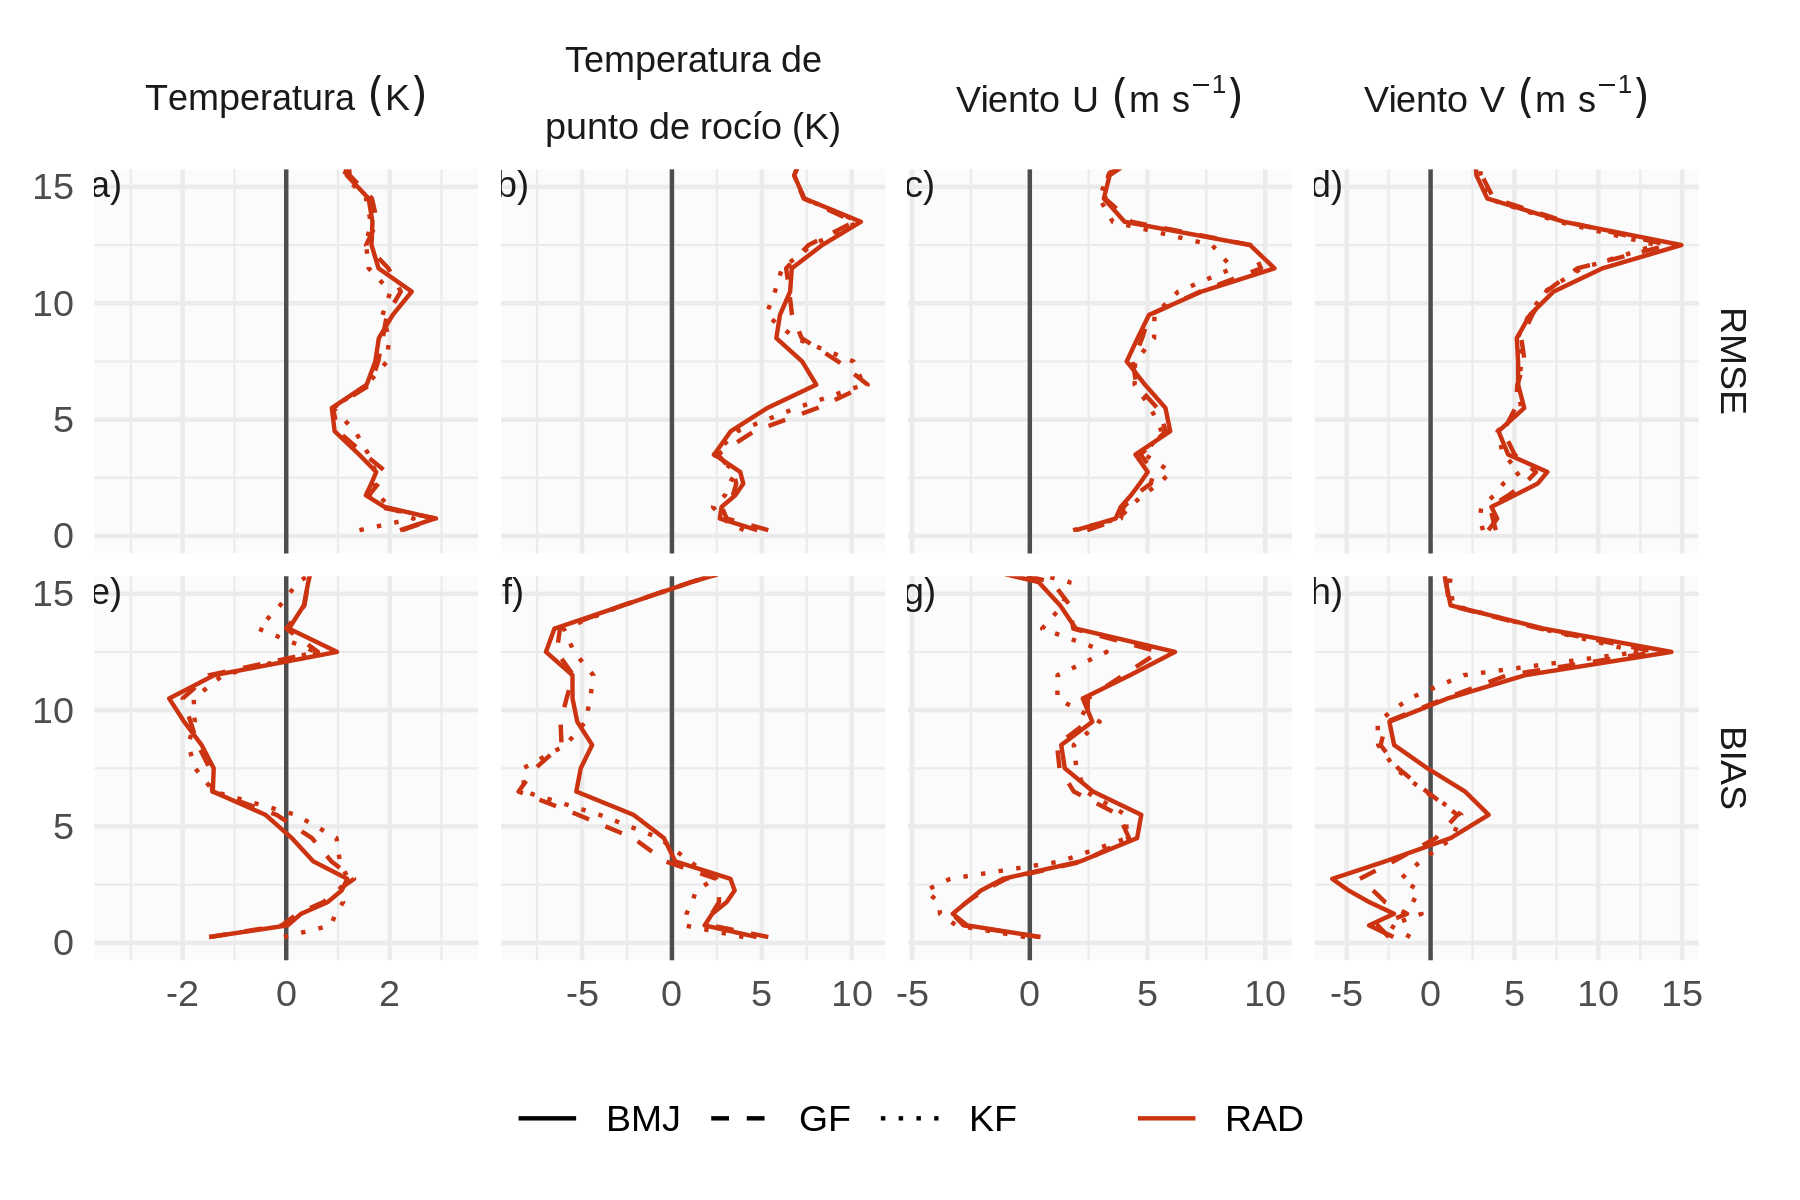
\includegraphics{thesis_files/figure-latex/souding-rad-1} 

}

\caption{RMSE y BIAS calculados comparando los pronósticos con observaciones de sondeos de RELAMPAGO y promediados sobre los miembros del ensamble que utilizan las parametrizaciones de conveccón BMJ (línea llena), GF (línea a rayas) e KF (línea punteada) para todos los pronósticos en conjunto.}\label{fig:souding-rad}
\end{figure}

\begin{figure}
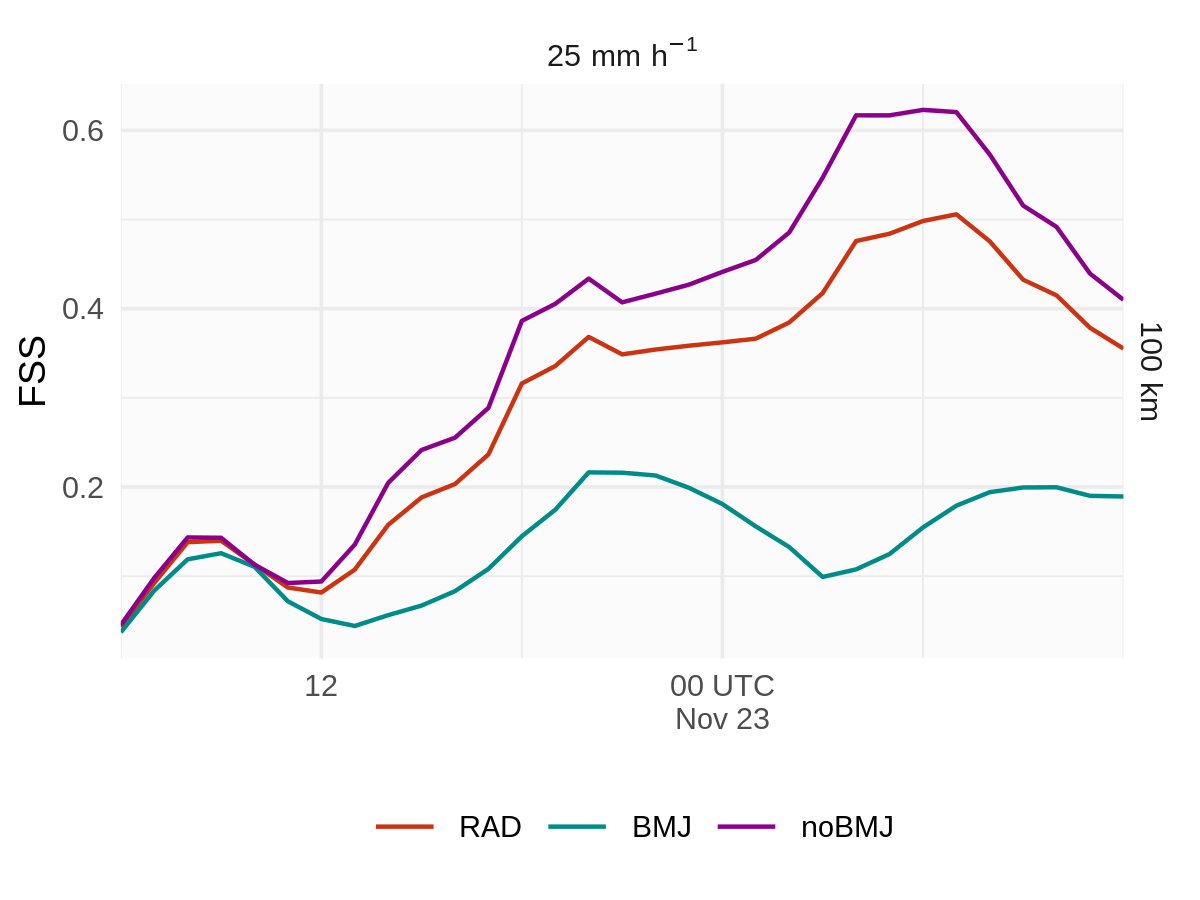
\includegraphics{thesis_files/figure-latex/fss-bmj-1} \caption{FSS calculado sobre la precipitación acumulada a 1 hora en una ventana móvil de 6 horas para el umbral de 25 mm y 100 km de escala sobre el pronóstico RAD inicializado a las 00 UTC. La línea roja (RAD) corresponde al ensamble completo, la línea turquesa (BMJ) se calcula sobre los miembros del ensamble que usan la parametrización de convección BMJ y la línea violeta (noBMJ) se calcula sobre los miembros del ensamble que no utilizan BMJ.}\label{fig:fss-bmj}
\end{figure}
\hypertarget{conclusiones-1}{%
\section{Conclusiones}\label{conclusiones-1}}

\hypertarget{asimilacion-de-observaciones-del-satuxe9lite-geoestacionario-goes-16}{%
\chapter{Asimilacion de observaciones del satélite geoestacionario GOES-16}\label{asimilacion-de-observaciones-del-satuxe9lite-geoestacionario-goes-16}}

En este capítulo se evaluará el impacto que genera la asimilación de observaciones del sensor ABI a bordo del satélite GOES-16 tanto en el análisis como en pronósticos determinísticos de alta resolución para el caso de estudio del 22 de noviembre de 2018. Estas observaciones son de particular interés en la región de Sudamérica por su alta resolución espacial y frecuencia temporal. Las observaciones de los canales sensibles al vapor de agua, brindan además, información en 3 niveles de la atmósfera, algo que no era posible con los sensores previos a bordo de los satélites GOES. Esperamos que la asimilaci'on de estas observaciones contribuya a mejorar la representación de los procesos convectivos y de mesoescala en pronósticos a corto plazo.

Por ser un satélite y sensor nuevos, la última versión de GSI (V3.7) que fue publicada en julio de 2018 no incluye la posibilidad de asimilar estas observaciones. Fue necesario, entonces, modificar el código fuente del sistema de asimilación para incluir las rutinas necesarias utilizando como base los trabajos previos de Lee et al. (2019) y Liu et al. (2019). También por esta razón, el capítulo incluirá el análisis de experimentos para definir la mejor configuración posible y evaluar técnicamente la asimilación de observaciones de ABI.

\hypertarget{metodologuxeda-2}{%
\section{Metodología}\label{metodologuxeda-2}}

\hypertarget{asim-goes}{%
\subsection{Asimilación de observaciones de goes}\label{asim-goes}}

La asimilación directa de radianzas de ABI requiere las mismas consideraciones descriptas previamente en la sección \ref{asim-rad} en cuanto a control de calidad, corrección de bias, thnning e indentificación de pixeles nubosos. En esta sección se describiran las deciciones metodológicas y técnicas que se tomaron a la hora de asimilar las observaciones, en base a las pruebas preliminares realizadas.

Si bien las radianzas de satélite pueden tener errores sistemáticos asociados a las condiciones de la atmósfera, la geometría de observación y condiciones específicas de los sensores que deben ser corregidos previo a la asimilación, para este trabajo se generó una primera prueba de asimilación para evaluar la magnitud de estos errores. Esta primera prueba utiliza la misma configuración de modelo y ensamble que los experimentos discutidos previamente e incluye la asimilación de los 3 canales de ABI en conjunto.

La Figura \ref{fig:oma-dist} muestra la distribución de la diferencia entre las observaciones y el campo preliminar (OmF) y entre las observaciones y el análisis (OmA) para todo el periodo. Si las observaciones no tienen bias la distribución OmF estará centrada en cero. En este caso solo el canal 9 presenta un bias positivo muy pequeño del orden de 0.3 K (Tabla \ref{tab:oma-tabla}). Por esta razón no se hará corrección del bias a estas observaciones.

La Figura \ref{fig:oma-dist} y la Tabla \ref{tab:oma-tabla} muestran además otro resultado importante. Si la asimilación de las observaciones se realizó correctamente es esperable que la diferencia OmA esté más cerca de cero que OmF y que su distribución tenga menos varianza. Esto se observa para los 3 canales asimilados y confirma que la implementación técnica dentro del sistema funciona correctamente. Notar que los cambios abruptos y simétricos en las curvas de distribución se deben al chequeo preliminar que se realiza como parte de los controles de calidad y que elimina aquellas observaciones que tienen un diferencia mayor a 2.2 K con respecto del campo preliminar.


\begin{figure}

{\centering 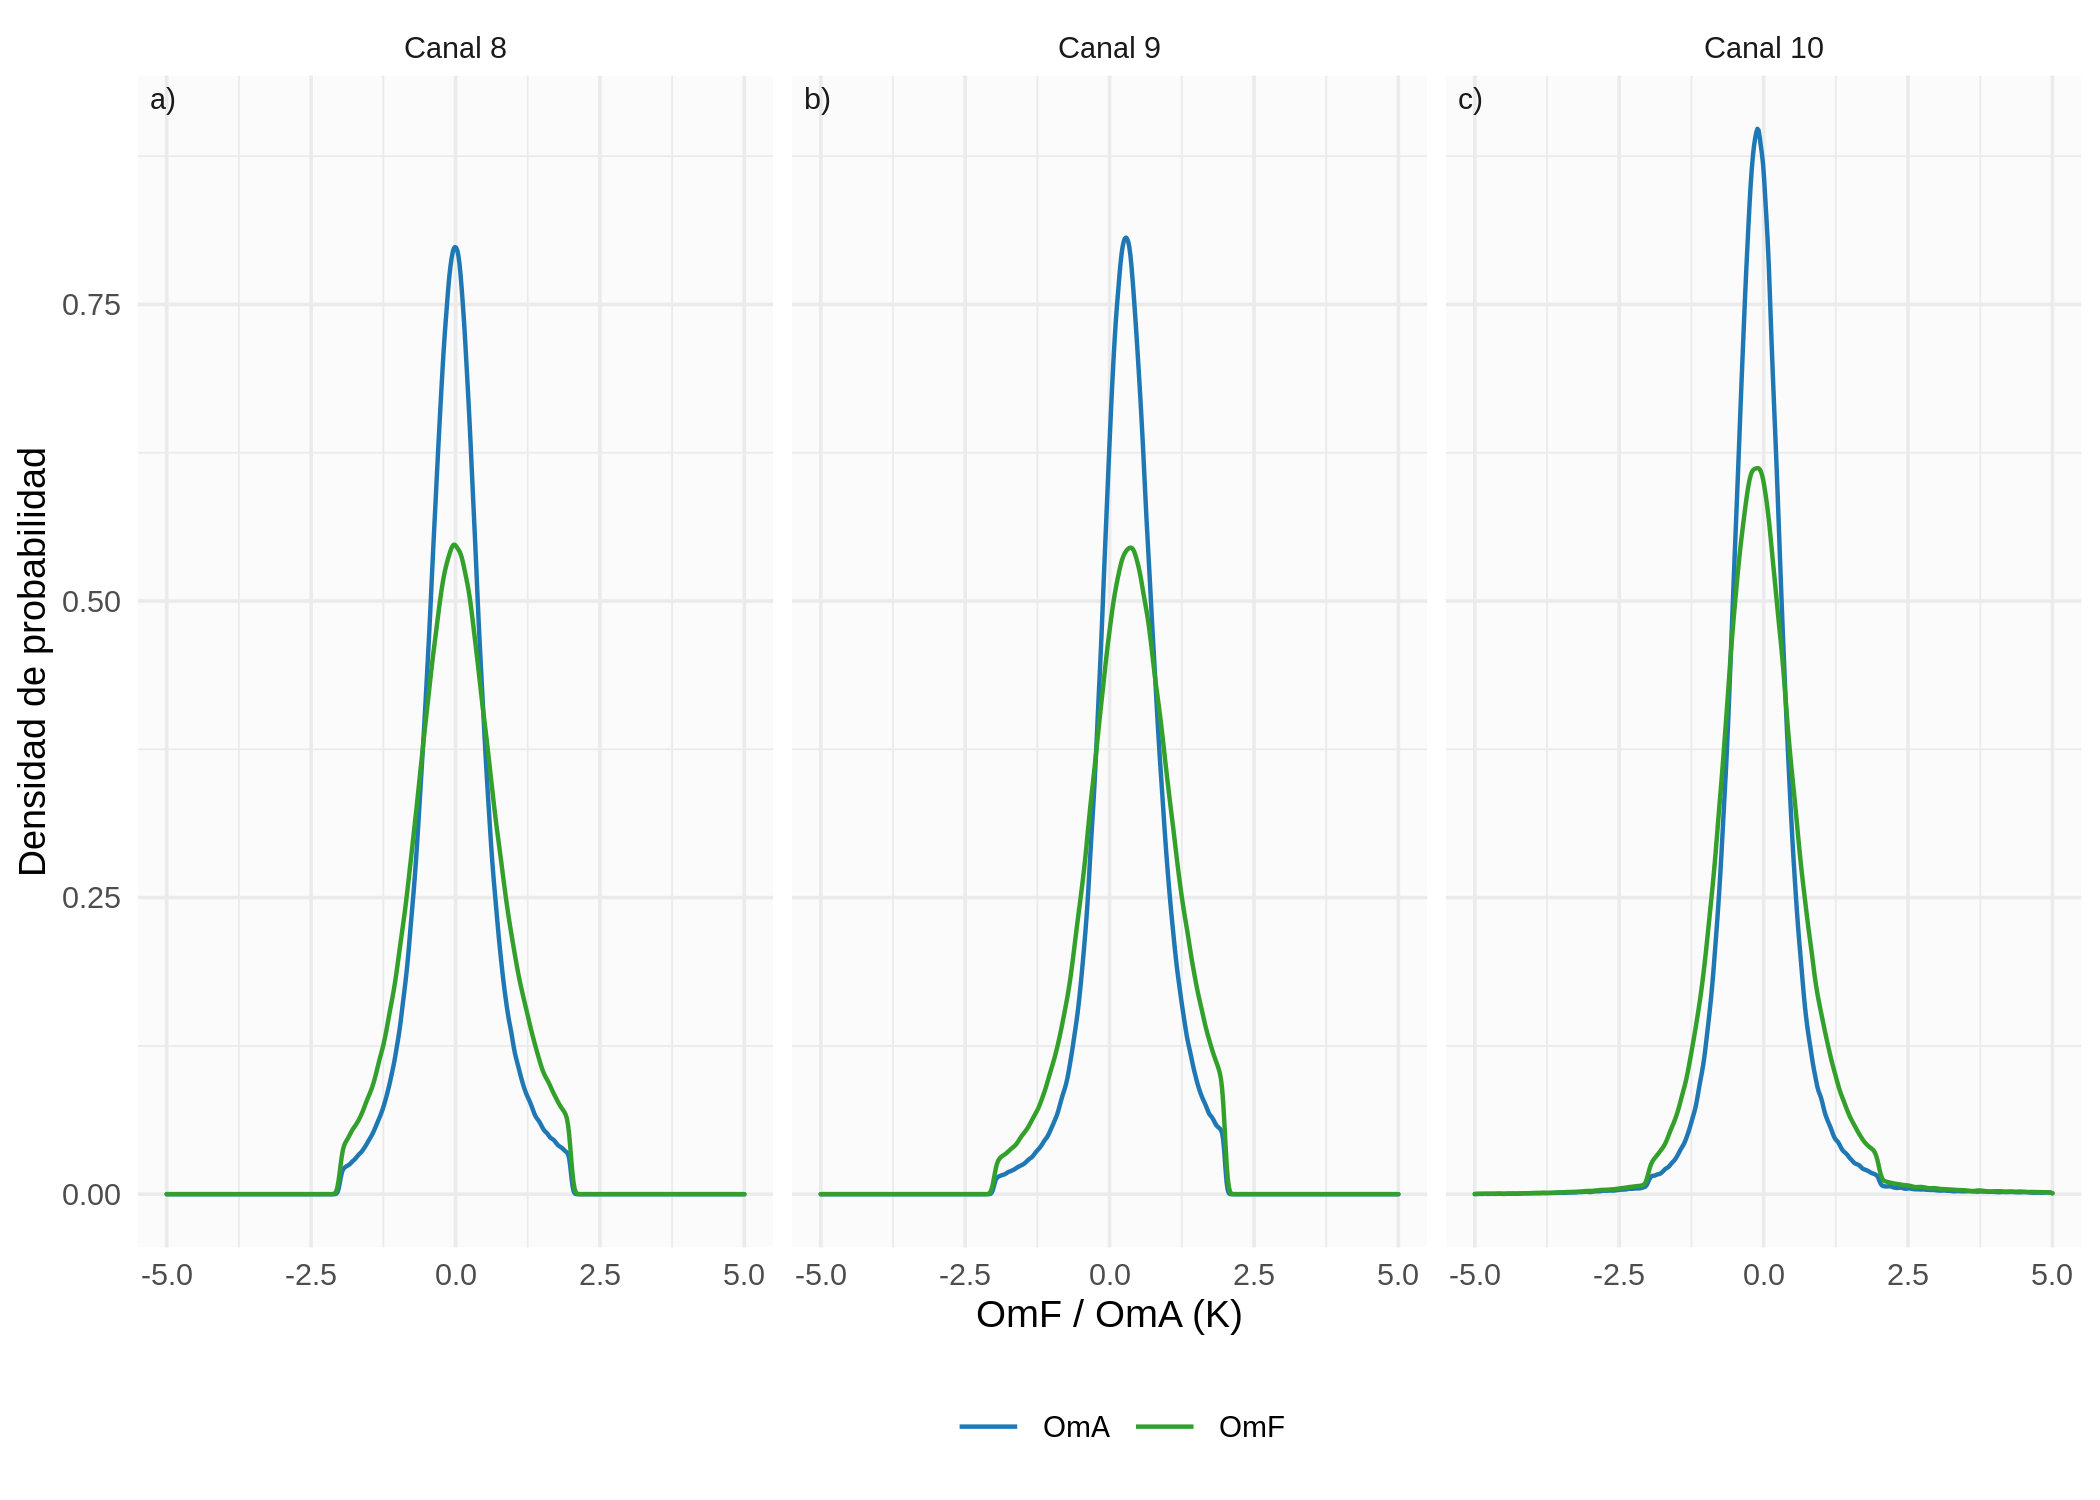
\includegraphics{thesis_files/figure-latex/oma-dist-1} 

}

\caption{Distribución de la diferencia entre las observaciones y el campo preliminar (OmF) y la observacion y el análisis (OmA) para los 3 canales de ABI y a lo largo de todo el periodo de prueba.}\label{fig:oma-dist}
\end{figure}
\begin{table}

\caption{\label{tab:oma-tabla}Observación menos análisis o campo preliminar medio calculado sobre todo el periodo.}
\centering
\begin{tabu} to \linewidth {>{\raggedright}X>{\raggedleft}X>{\raggedleft}X>{\raggedleft}X}
\toprule
 & Canal 8 & Canal 9 & Canal 10\\
\midrule
OmF & 0.0355 & 0.3212 & -0.0158\\
OmA & 0.0032 & 0.3140 & -0.0498\\
\bottomrule
\end{tabu}
\end{table}
La asimilación de radianzas en \emph{all sky}, es decir tanto para cielos claros como nubosos es todavía un importante desafío ya que estos dos tipos de observaciones requieren un control de calidad y estimaciones de errores específicos. En esta primera aproximación a la asimilación de observaciones de ABI solo se utilizaron observaciones en cielo claro. Para detectar y filtrar los pixeles nubosos utilizamos la mascara de nubes ACM (por ABI Cloud Mask) disponible con la misma frecuencia que las observaciones. Esta mascara de nubes da información binaria (cielo claro o cielo nuboso) y tienen una exactitud del 87\%. La estimación es realizada utilizando información de 10 canales de ABI e incluye pruebas espectrales, espaciales y temporales. En las Figuras \ref{fig:cld-msk} se presentan 2 ejemplos de máscara de nubes a las 00 UTC del 20 de noviembre y a las 18 UTC del 22 de noviembre.


\begin{figure}
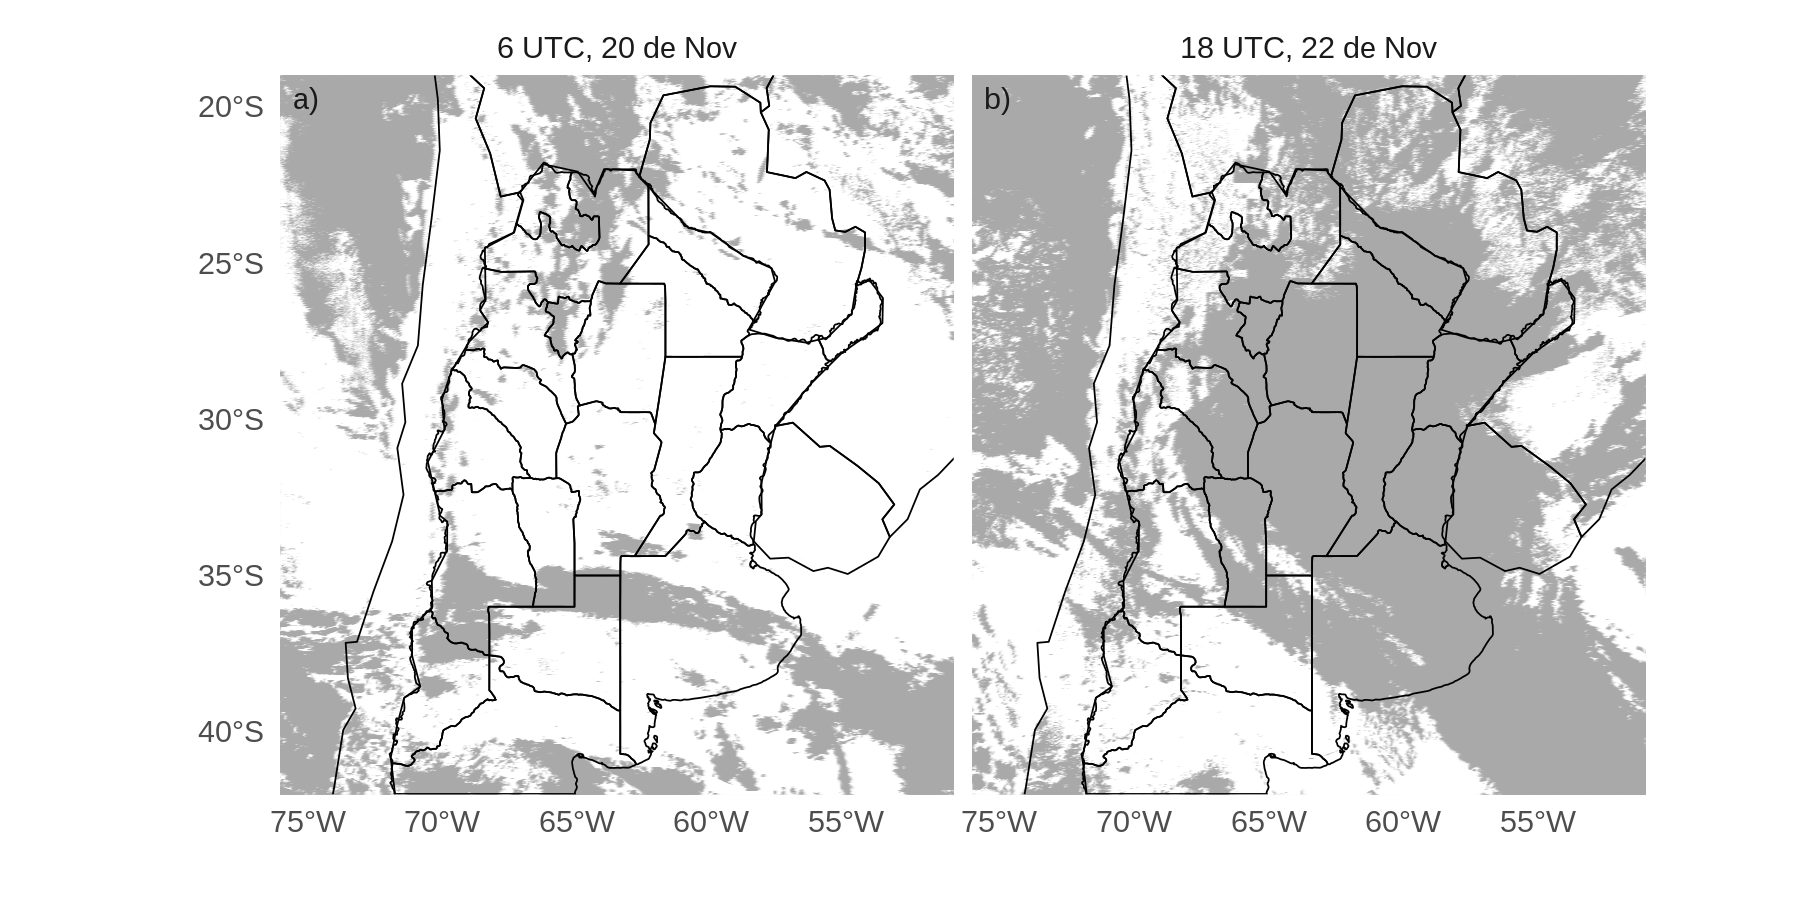
\includegraphics{thesis_files/figure-latex/cld-msk-1} \caption{Ubicación de píxeles nubosos (gris) según la máscara de nubes generada como producto de nivel 2 para GOES-16, durante el a) 06 UTC del 20 de noviembre y b) 18 UTC del 22 de noviembre.}\label{fig:cld-msk}
\end{figure}
Debido al desarrollo de actividad convectiva en el dominio durante el periodo simulado, la cantidad de observaciones en cielo claro varía considerablemente. Esto puede apreciarse en las Figuras \ref{fig:cld-msk} a y b. Sin embargo la cantidad de observaciones que aporta ABI es casi siempre superior a las observaciones de satélites polares (Figura \ref{fig:obs-rad}a) .


\begin{figure}
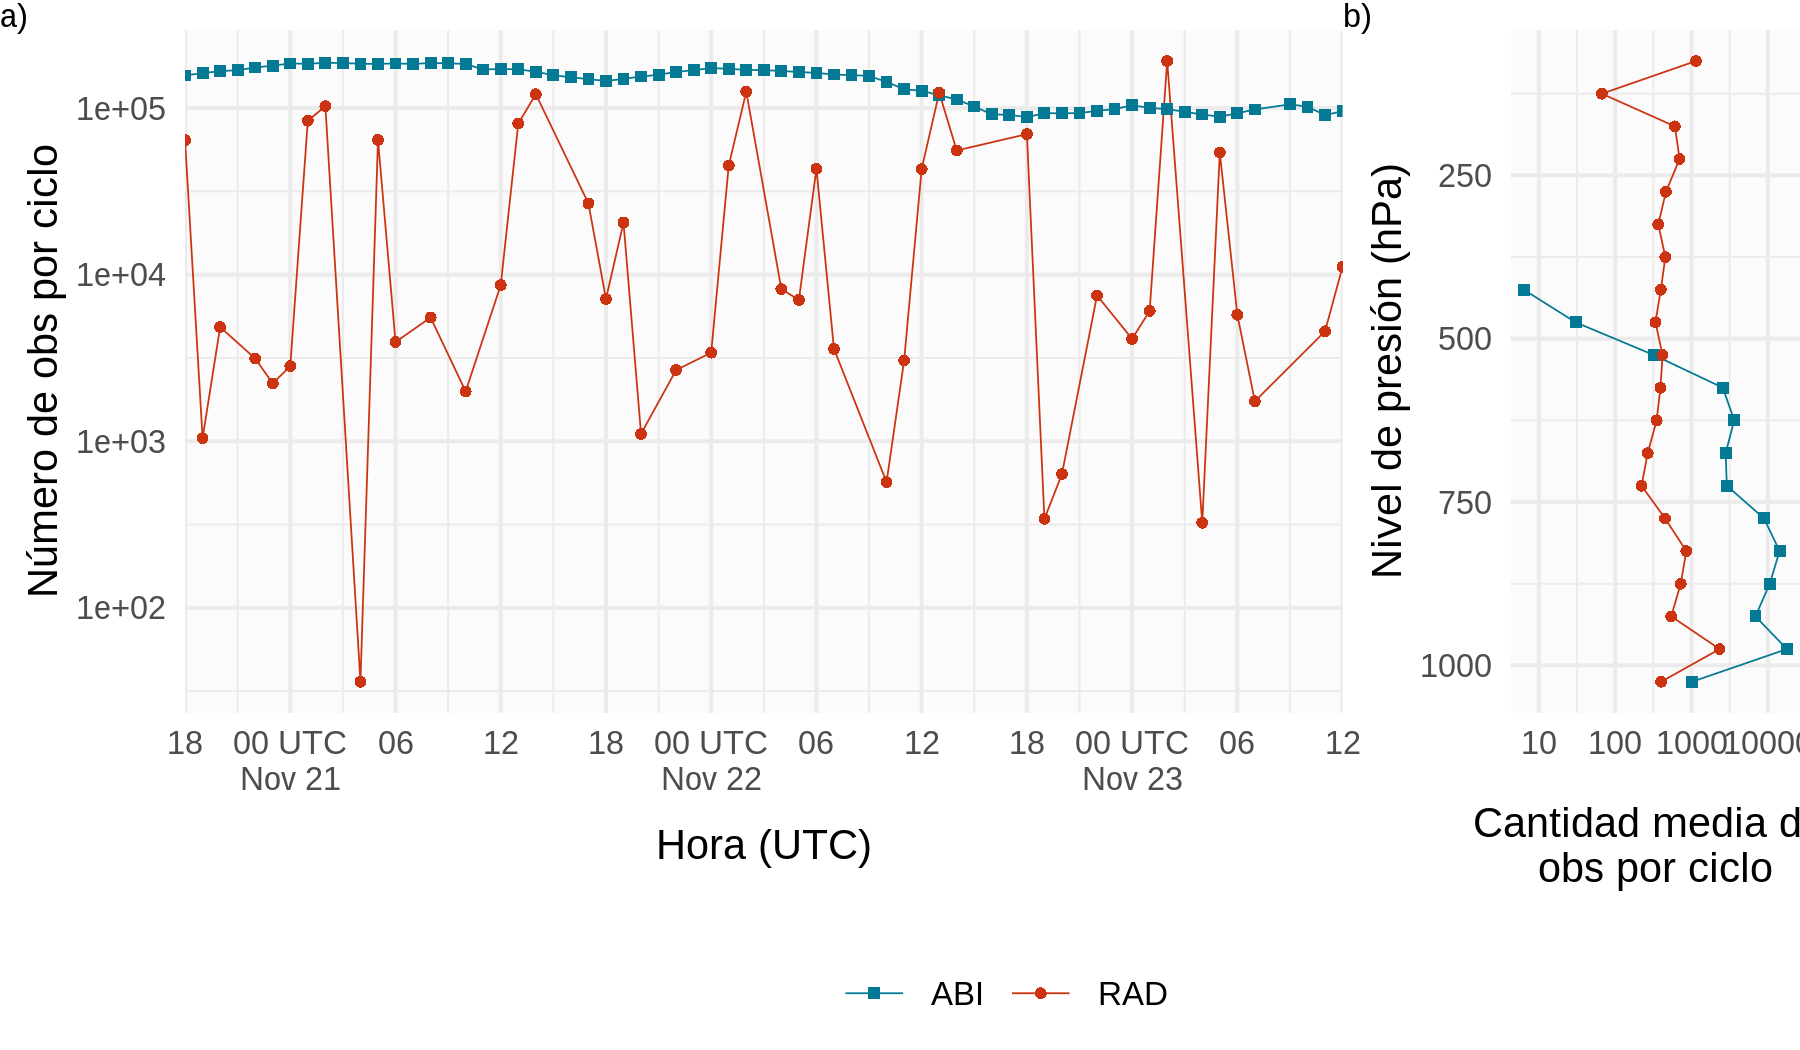
\includegraphics{thesis_files/figure-latex/obs-rad-1} \caption{a) Número de radianzas asimiladas en cada ciclo y b) número medio de radianzas asimiladas por ciclo en capas verticales de 50 hPa de espesor para los experimentos RAD (radianzas de satélites polares, circulos rojos) y ABI (radianzas de ABI, cuadrados turquezas).}\label{fig:obs-rad}
\end{figure}
\hypertarget{configuracion-de-los-experimentos-1}{%
\subsection{Configuracion de los experimentos}\label{configuracion-de-los-experimentos-1}}

En este capítulo se analizan una serie de experimentos, primero para evaluar la sensibilidad a distintas combinaciones de canales y a la resolución del thinning y finalmente para comparar el impacto de la asimilación de observaciones de ABI en conjunto o no con observaciones de satélites polares. Los experimentos SATWND y RAD fueron analizados previamente en el capítulo \ref{ch1}. SATWND asimila observaciones de EMC, EMA y vientos deriados de satélite y RAD suma a lo anterior radianzas en aire claro de sensores a bordo de satélites polares. RAD+ABI incluye además observaciones de los 3 canales de vapor de agua de ABI con un thinning de 10 km. Finalmente el conjunto de experimentos ABI incluye radianzas de ABI pero no de satélites polares, y usan distintas combinaciones de canales y resolución de thinning (Tabla \ref{tab:exp-rad}).
\begin{table}

\caption{\label{tab:exp-rad}Experimentos realizados. Todos los experimentos incluyen observaciones de EMC, EMA y vientos derivados de satélite. }
\centering
\begin{tabu} to \linewidth {>{\raggedright\arraybackslash}p{8em}>{\raggedright\arraybackslash}p{20em}>{\centering\arraybackslash}m{4em}>{\centering\arraybackslash}m{4em}}
\toprule
Experimento & Radianzas asimiladas & Canales ABI & Thining ABI\\
\midrule
SATWND & -- & -- & --\\
RAD & Radianzas de satélites polares & -- & --\\
RAD+ABI & Radianzas de satélites polares y ABI & 8, 9, 10 & 10 km\\
ABI\_ch890\_th10 (ABI) & Radianzas de ABI & 8, 9, 10 & 10 km\\
ABI\_ch890\_th30 & Radianzas de ABI & 8, 9, 10 & 30 km\\
\addlinespace
ABI\_ch90\_th30 & Radianzas de ABI & 9, 10 & 30 km\\
ABI\_ch0\_th30 & Radianzas de ABI & 10 & 30 km\\
\bottomrule
\end{tabu}
\end{table}
Todos los experimentos previamente descriptos usan la configuración del ensamble multifísica y del sistema de asimilación explicada en la sección \ref{configmodelo}. De la misma manera los ciclos de análisis horarios se realizan desde las 18 UTC del 20 de noviembre hasta las 12 UTC del 23 de noviembre para cubrir el desarrollo y maduración del SCM.

Para estudiar el impacto de la asimilación de radianzas también se generaron pronósticos determinísticos en alta resolución inicializados a las 00 y 06 UTC del 22 de noviembre (Figura \ref{fig:cycle-fcst}). En la Figura \ref{fig:dominio-det} se muestra el dominio \emph{d01} con 10 km de resolución (línea negra), identico al dominio utilizado para el resto de las simulaciones num'ericas y el dominio anidado \emph{d02} con 2 km de resolución (línea turquesa). Las condiciones iniciales están dadas por los análisis de los distintos experimentos y las condiciones de borde son generadas a partir del GFSF determinístico. Además las variables atmosféricas para el \emph{d02} fueron inicializadas haciendo un escalado de la información del análisis. Todos los pronósticos utilizan las mismas parametrizaciones: del modelo de superficie terrestre (Noah-MP, Chen and Dudhia (2001)), de microfísica (esquema de un solo momento de 6 clases del WRF, Hong, Noh, et al. (2006)) de procesos radiativos (esquema de onda corta y onda larga del RRTMG, Iacono et al. (2008)), YSU (Hong, Kim, et al., 2006) para capa límite y KF (Kain, 2004) para covección (solo aplicado al \emph{d01}).

Además de los pronósticos inicializados a partir de los análisis, se generaron pronósticos inicializados a partir de GFS, es decir, sin asimilación de datos regional. Estos pronósticos tienen la misma configuración y usan el mismo conjunto de parametrizaciones que los los pronósticos descriptos previamente.


\begin{figure}

{\centering 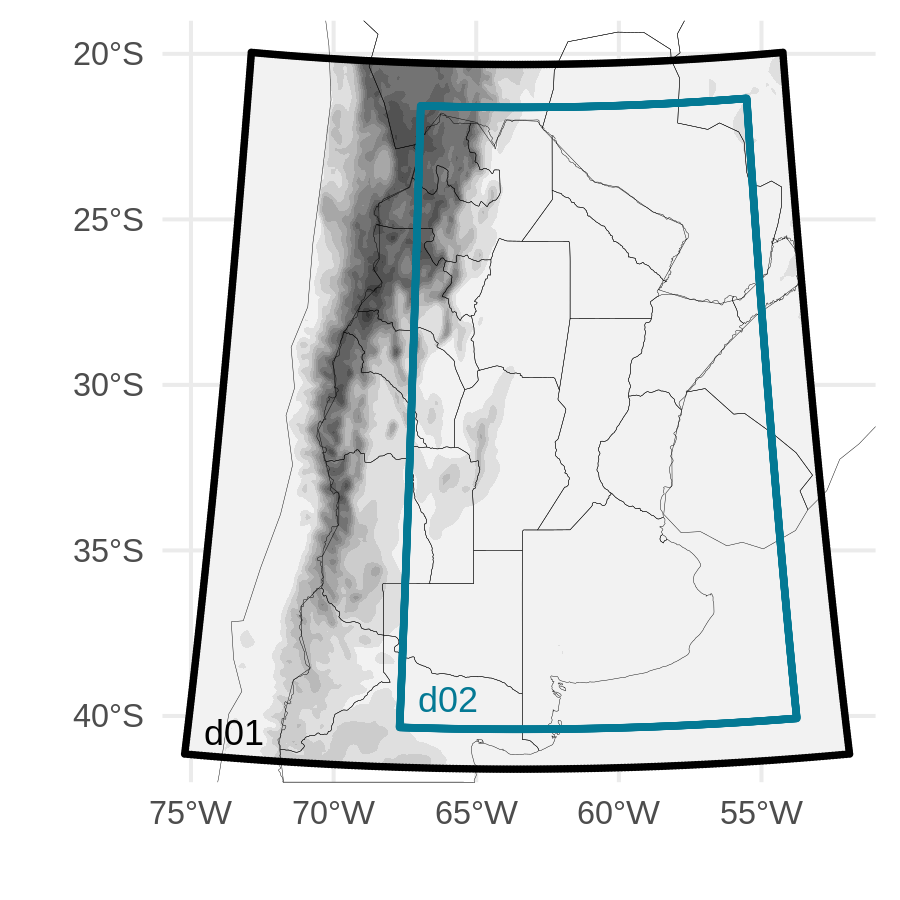
\includegraphics{thesis_files/figure-latex/dominio-det-1} 

}

\caption{Dominio de baja resolución (d01, 10 km) marcado con un recuadro negro y dominio anidado de alta resolución (d02, 2 km) marcado en color turquesa.}\label{fig:dominio-det}
\end{figure}
\hypertarget{resultados-2}{%
\section{Resultados}\label{resultados-2}}

\hypertarget{canales}{%
\subsection{Sensibilidad a la combinación de canales}\label{canales}}

Trabajos previos evaluaron el impacto de asimilar observaciones de los canales asociados al vapor de agua de ABI en escala regional. En líneas general estos trabajos (por ejemplo Lee et al. (2019), Jones et al. (2020)) utilizan las observaciones de los 3 canales en conjunto. Sin embargo ({\textbf{???}}) encontraron mejores resultado al asimilar los canales 8 (6.2 \(\mu m\)) y 10 (7.3 \(\mu m\)) observando que el cnal 9 (6. \(\mu m\)) está muy correlacionado con los otros dos y por lo tanto no aporta información independiente en la asimilación. Por otro lado Lee et al. (2019) observaron que el impacto era mayor al asimilar observaciones de los 3 canales sobre el continente y el mar al mismo tiempo. También observaron que el incremento del análisis disminuye considerablemente al remover el canal 10 y en algunos casos también el canal 9.

En este trabajo se generaron 3 experimentos de prueba que comparten la misma configuración que los experimentos previamente descriptos pero utilizando distintas combinaciones de canales de ABI. El experimento ABI\_ch890\_th30 asimila observaciones de los 3 canales, ABI\_ch90\_th30 asimila observaciones de los 9 y 10 (vapor de agua en niveles medios y bajos respectivamente) y ABI\_ch0\_th30 solo utliza observaciones del canal 10. Estos 3 experimentos utilizan un thinning de 30 km como primera aproximación, un análisis más detallado del thinning se realizará en la siguiente sección.


\begin{figure}
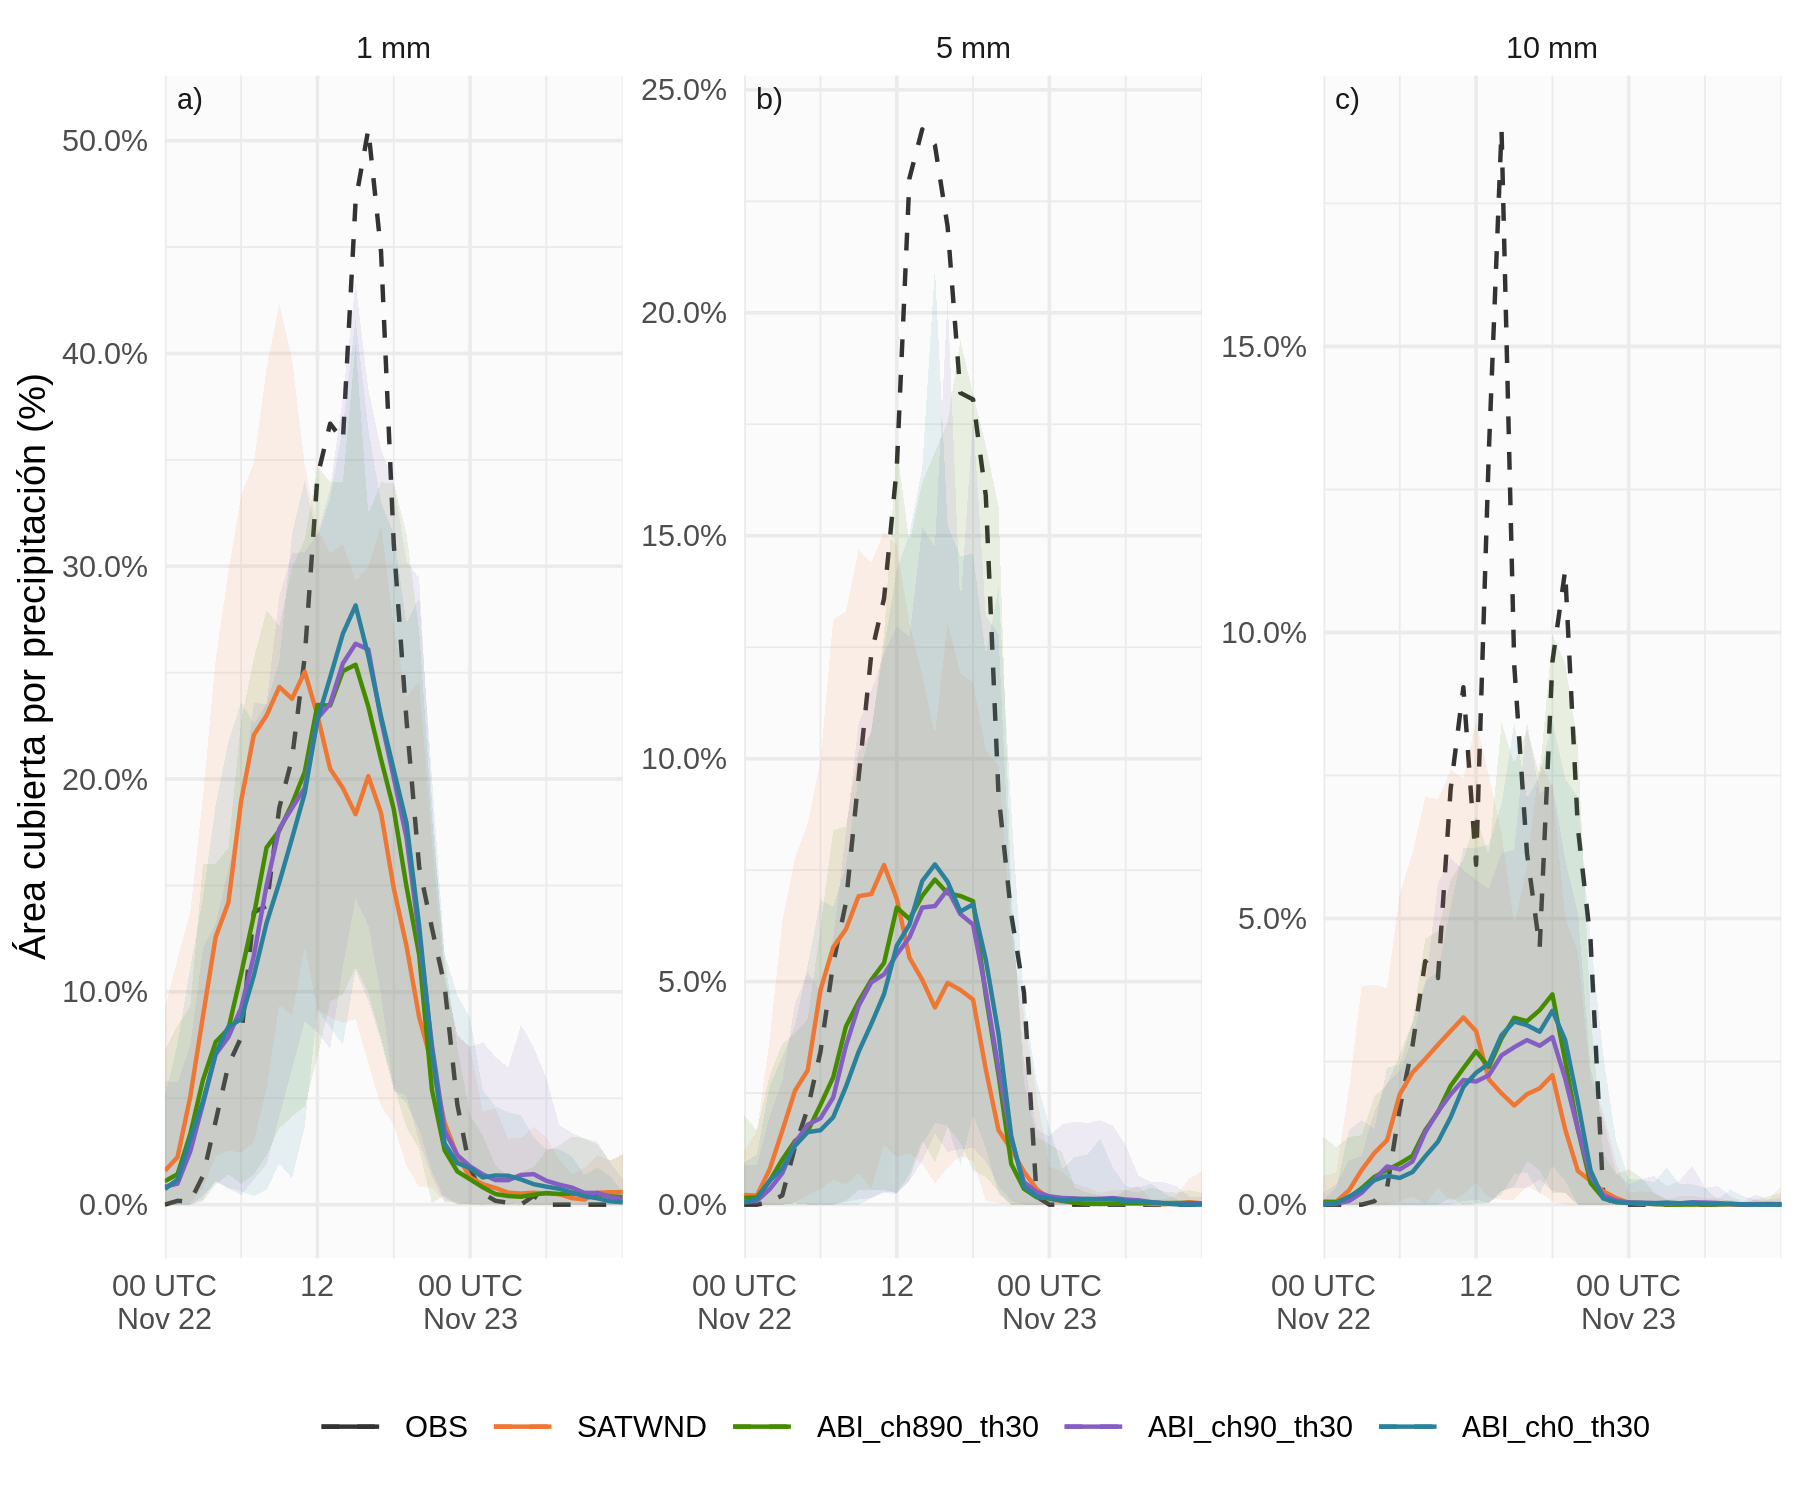
\includegraphics{thesis_files/figure-latex/area-canales-1} \caption{Porcentaje de área cubierta por precipitación a 1 hora superior a a) \(1 mmh^{-1}\), b) \(5 mmh^{-1}\) y c) \(10 mmh^{-1}\) a lo largo del tiempo para el campo preliminar de los experimentos SATWND (línea naranja), ABI\_ch890\_th30 (línea verde), ABI\_ch90\_th30 (línea violeta) y ABI\_ch0\_th30 (línea celeste) entre las 00 UTC del 22 de noviembre y las 12 UTC del 23 de noviembre en el dominio de verificación (cuadro rojo en la Figura \ref{fig:dominio}a). En sombreado y para cada experimento se muestra el área máxima y mínima estimada por el ensamble del análisis. En línea continua negra se muetra la estimación de IMERG.}\label{fig:area-canales}
\end{figure}
La Figura \ref{fig:area-canales} muestra el porcetanje de área cubierta por precipitación superior a distintos umbrales y compara los experimentos para estudiar la sensibilidad al uso de canales con SATWND como experimento control y la estimación de precipitación de IMERG. Al igual que en otros experimentos, los experimentos ABI subestiman la precipitación observada y tienen además un comportamiento similar a SATWND. En algunos casos, logran representar mejor la precipitación que SATWND particularmente para umbrales de precipitación mayores (Figura \ref{fig:area-canales}b-c) y algunas sub regiones como la provincia de Córdoba (no se muestra). Comparando los experimentos ABI entre si, no se observan grandes diferencias y solo en algunos casos ABI\_ch890\_th30 es mejor que otros otros dos. Desde este punto de vista la asimilación de las observaciones de los canales 8 y 9 en niveles altos y medios no aporta mucha información al análisis.

Desde el punto de vista del FSS (Figura \ref{fig:fss-canales}) los experimentos que incluyen observaciones de ABI tienen un rendimiento mucho mejor que SATWND. De manera similar los 3 experimentos de ABI tienen un comportamiento similar aunque en este caso ABI\_ch890\_th30 representa ligeramente mejor la precipitación por encima de 25 mm (Figuras \ref{fig:fss-canales}byd).

Teniendo en cuenta que la asimilación de los 3 canales de ABI en conjunto no degradan el análisis y por el contrario, en algunos casos parecen tener un rendimiento mejor, para los experimentos de de este capítulo se asimilaran los 3 canales al mismo tiempo.


\begin{figure}
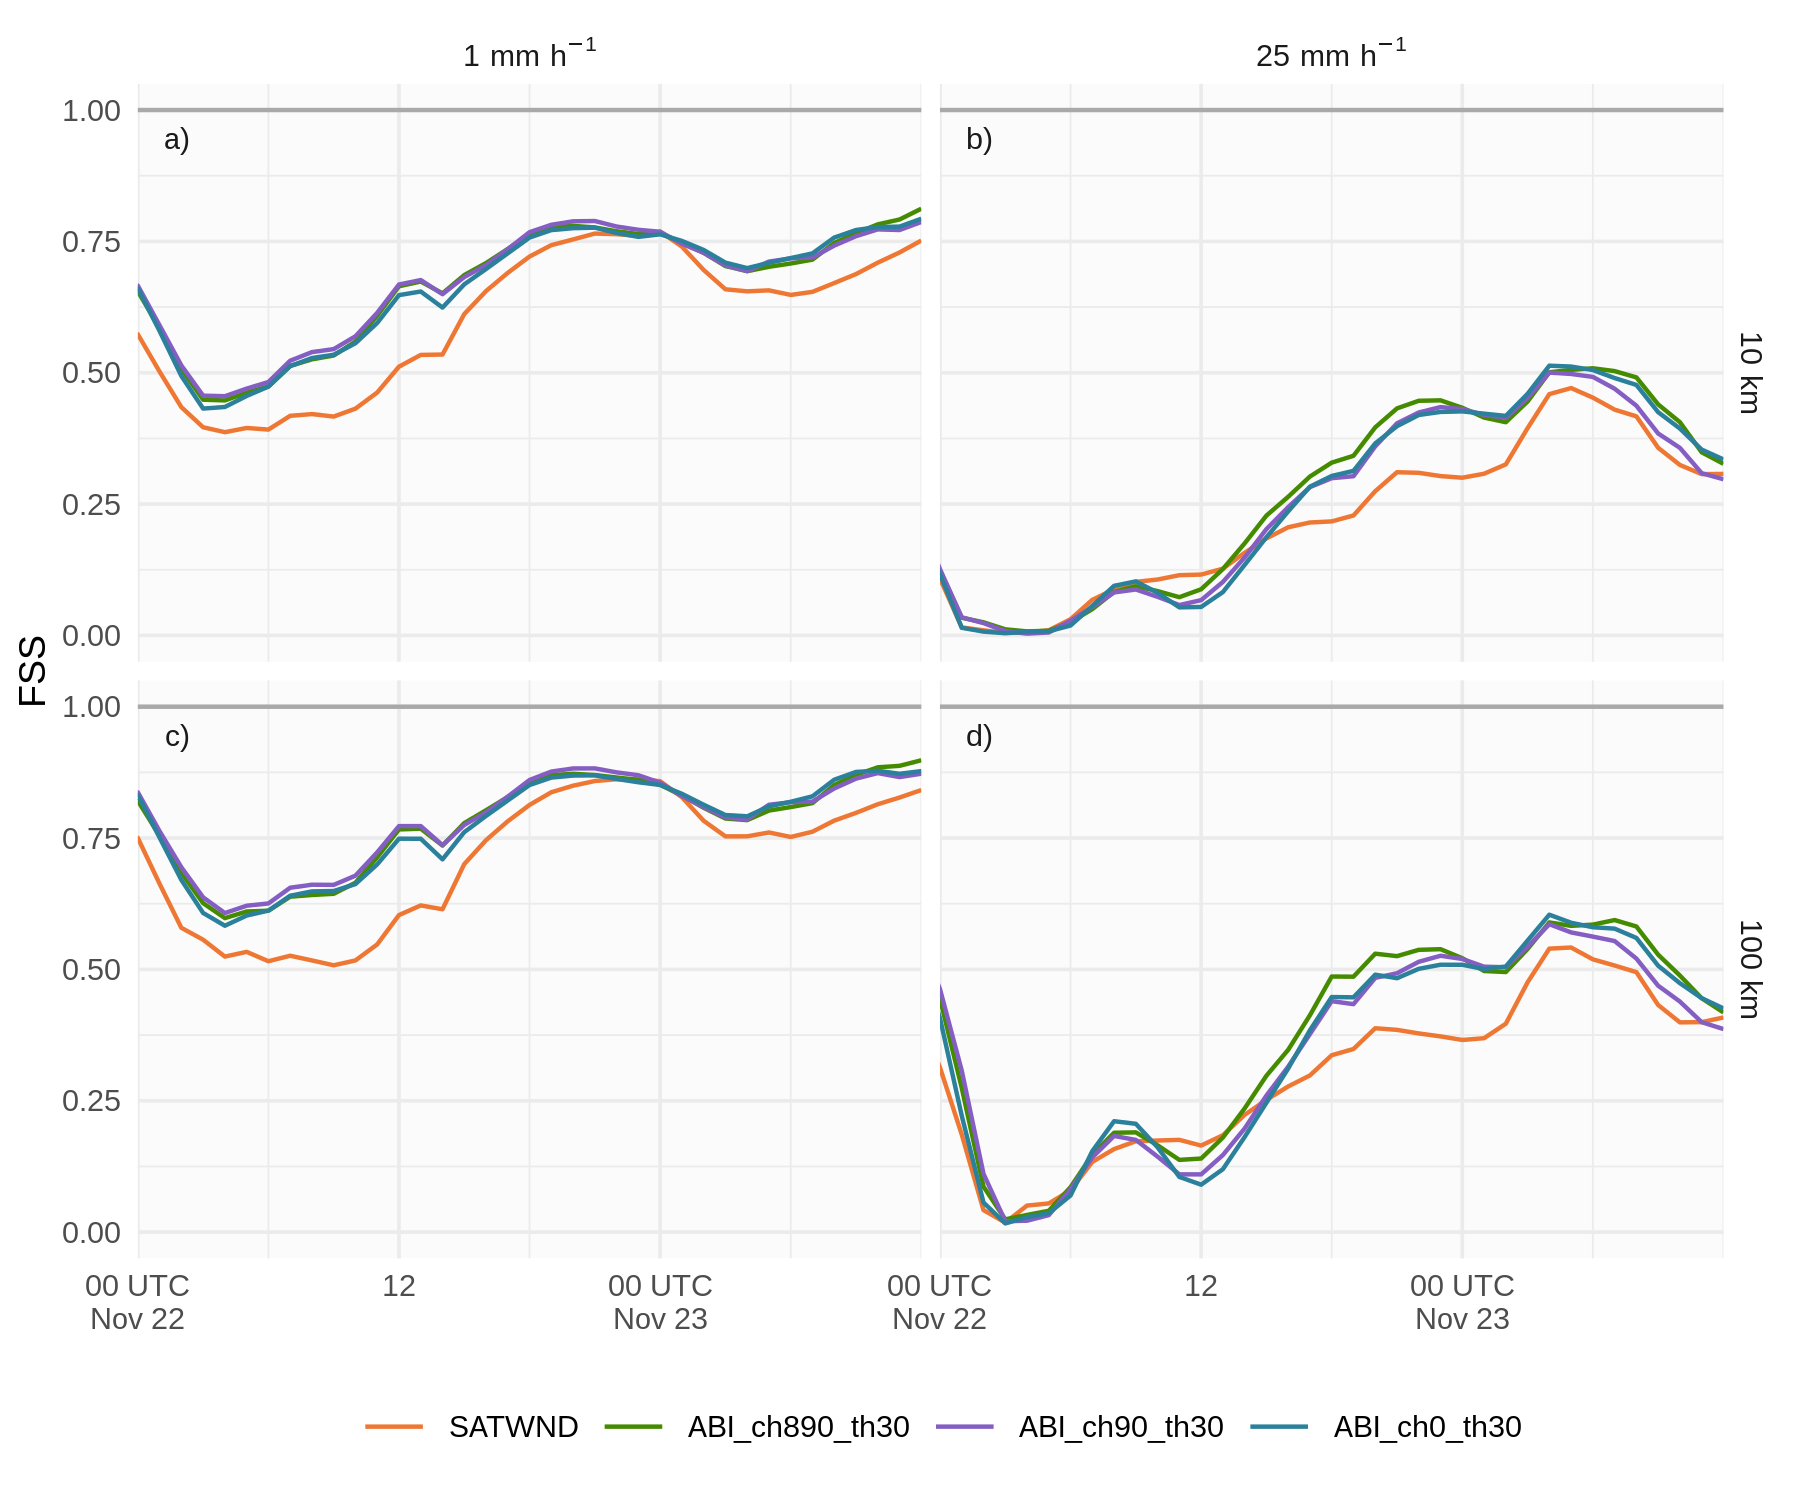
\includegraphics{thesis_files/figure-latex/fss-canales-1} \caption{FSS calculado sobre la precipitación acumulada a 1 hora en una ventana móvil de 6 horas para umbrales de 1 mm (a y c) y 25 mm (b y d), en escalas de 10 km (a y b) y 100 km (c y d), para el campo preliminar de los experimentos SATWND (línea naranja), ABI\_ch890\_th30 (línea verde), ABI\_ch90\_th30 (línea violeta) y ABI\_ch0\_th30 (línea celeste).}\label{fig:fss-canales}
\end{figure}
\hypertarget{thinning}{%
\subsection{Sensibilidad al thinning}\label{thinning}}

En la asimilación de datos y en particular de radianzas de satélites, muchas observaciones con alta resolución espacial son descatadas porque podrían tener un impacto negativo en el análisis. En los esquemas de asimilación actuales se asume que la matriz de covarianza de los errores de las observaciones \(R\) es diagonal, es decir, no hay correlación entre los errores de las distintas observaciones y cada observación es independiente. En este contexto estrategias como el thinning para disminuir la resolución de las observaciones conservando la información que aportan son claves.

Existen diversos algoritmos para realizar el thinning, GSI en particular utiliza una metodología simple que consiste en definir una retícula de baja resolución y seleccionar las observaciones en alta resolución según la distancia a los puntos de la retícula gruesa y criterios de calidad descriptos en la sección \ref{sat}.

Es importante definir entonces la resolución apropiada para la reticula de baja resolución y el impacto que esto tiene en el análisis. Para esto se realizaron 2 experimentos ABI\_ch890\_th30 con un thinning de 30 km, es decir, que lleva las observaciones con una resolución de 2 km a una reticula de 30 km, y ABI\_ch890\_th10 con un thinning de 10 km, igual a la resolución de las simulaciones.


\begin{figure}
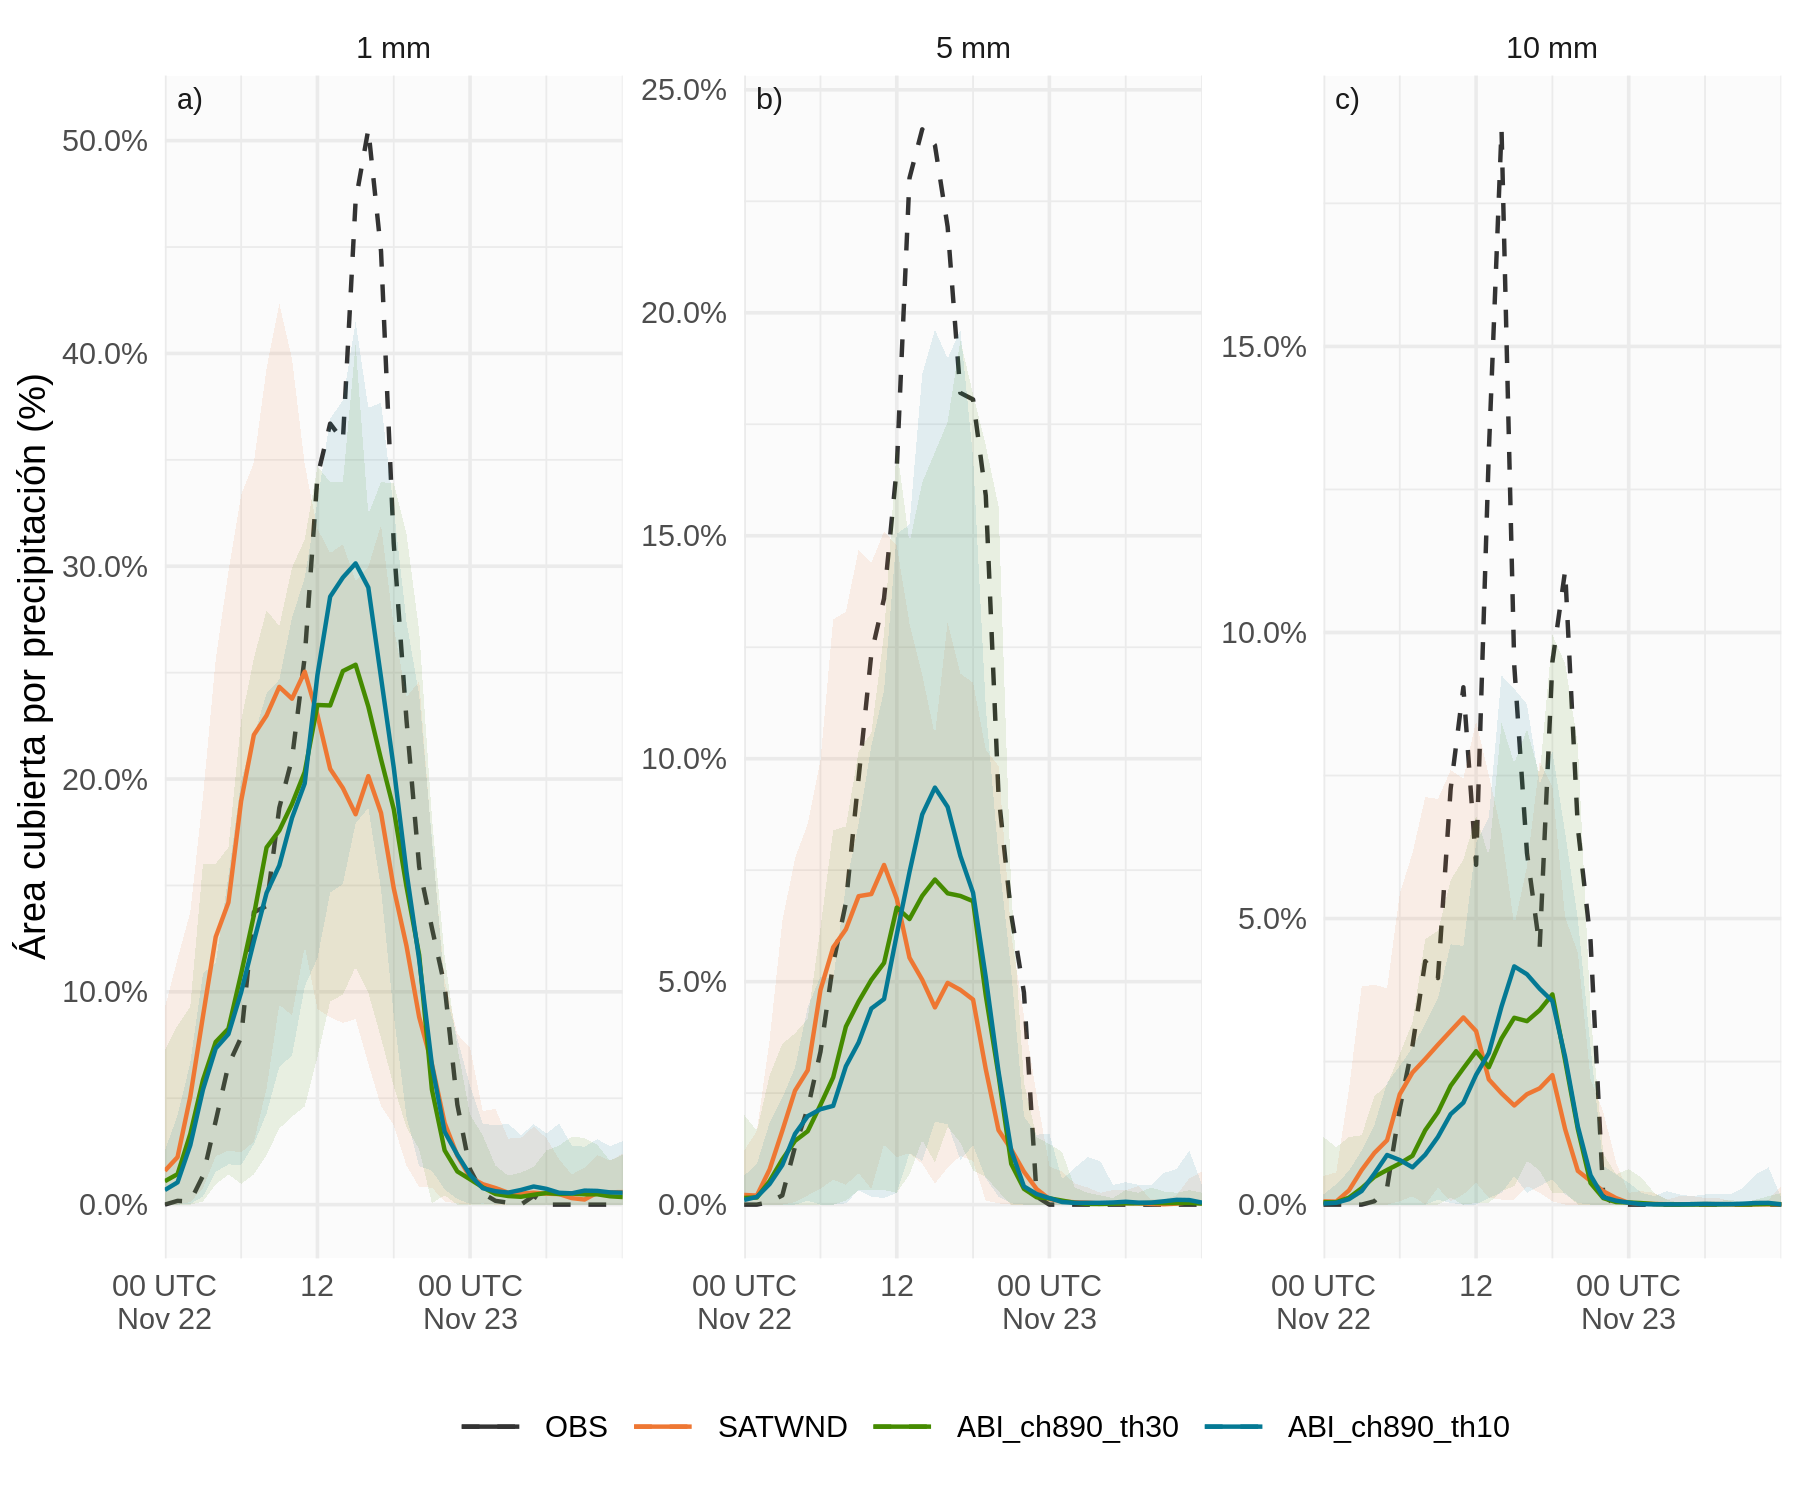
\includegraphics{thesis_files/figure-latex/area-thinning-1} \caption{Porcentaje de área cubierta por precipitación a 1 hora superior a a) \(1 mmh^{-1}\), b) \(5 mmh^{-1}\) y c) \(10 mmh^{-1}\) a lo largo del tiempo para el campo preliminar de los experimentos SATWND (línea naranja), ABI\_ch890\_th30 (línea verde), y ABI\_ch890\_th10 (línea celeste) entre las 00 UTC del 22 de noviembre y las 12 UTC del 23 de noviembre en el dominio de verificación (cuadro rojo en la Figura \ref{fig:dominio}a). En sombreado y para cada experimento se muestra el área máxima y mínima estimada por el ensamble del análisis. En línea continua negra se muetra la estimación de IMERG.}\label{fig:area-thinning}
\end{figure}
Comparamos los experimentos desde el punto de vista de la precipitación. En particular la Figura \ref{fig:area-thinning} muestra el porcentaje de área cubierta por precipitación superior a distintos umbrales a lo largo del tiempo para los experimentos de thinning y SATWND como experimento control. En todos los casos el experimento con un thinning de 10 km representa es el que mejor el área cuberta por precipitación, particularmente en las horas de mayor actividad convectiva. Si bien todos los experimentos subestiman la precipitación en comparación con IMERG, ABI\_ch890\_th10 se acerca a esta estimación sobre todo cuando observamos el área máxima del ensamble.
\begin{figure}
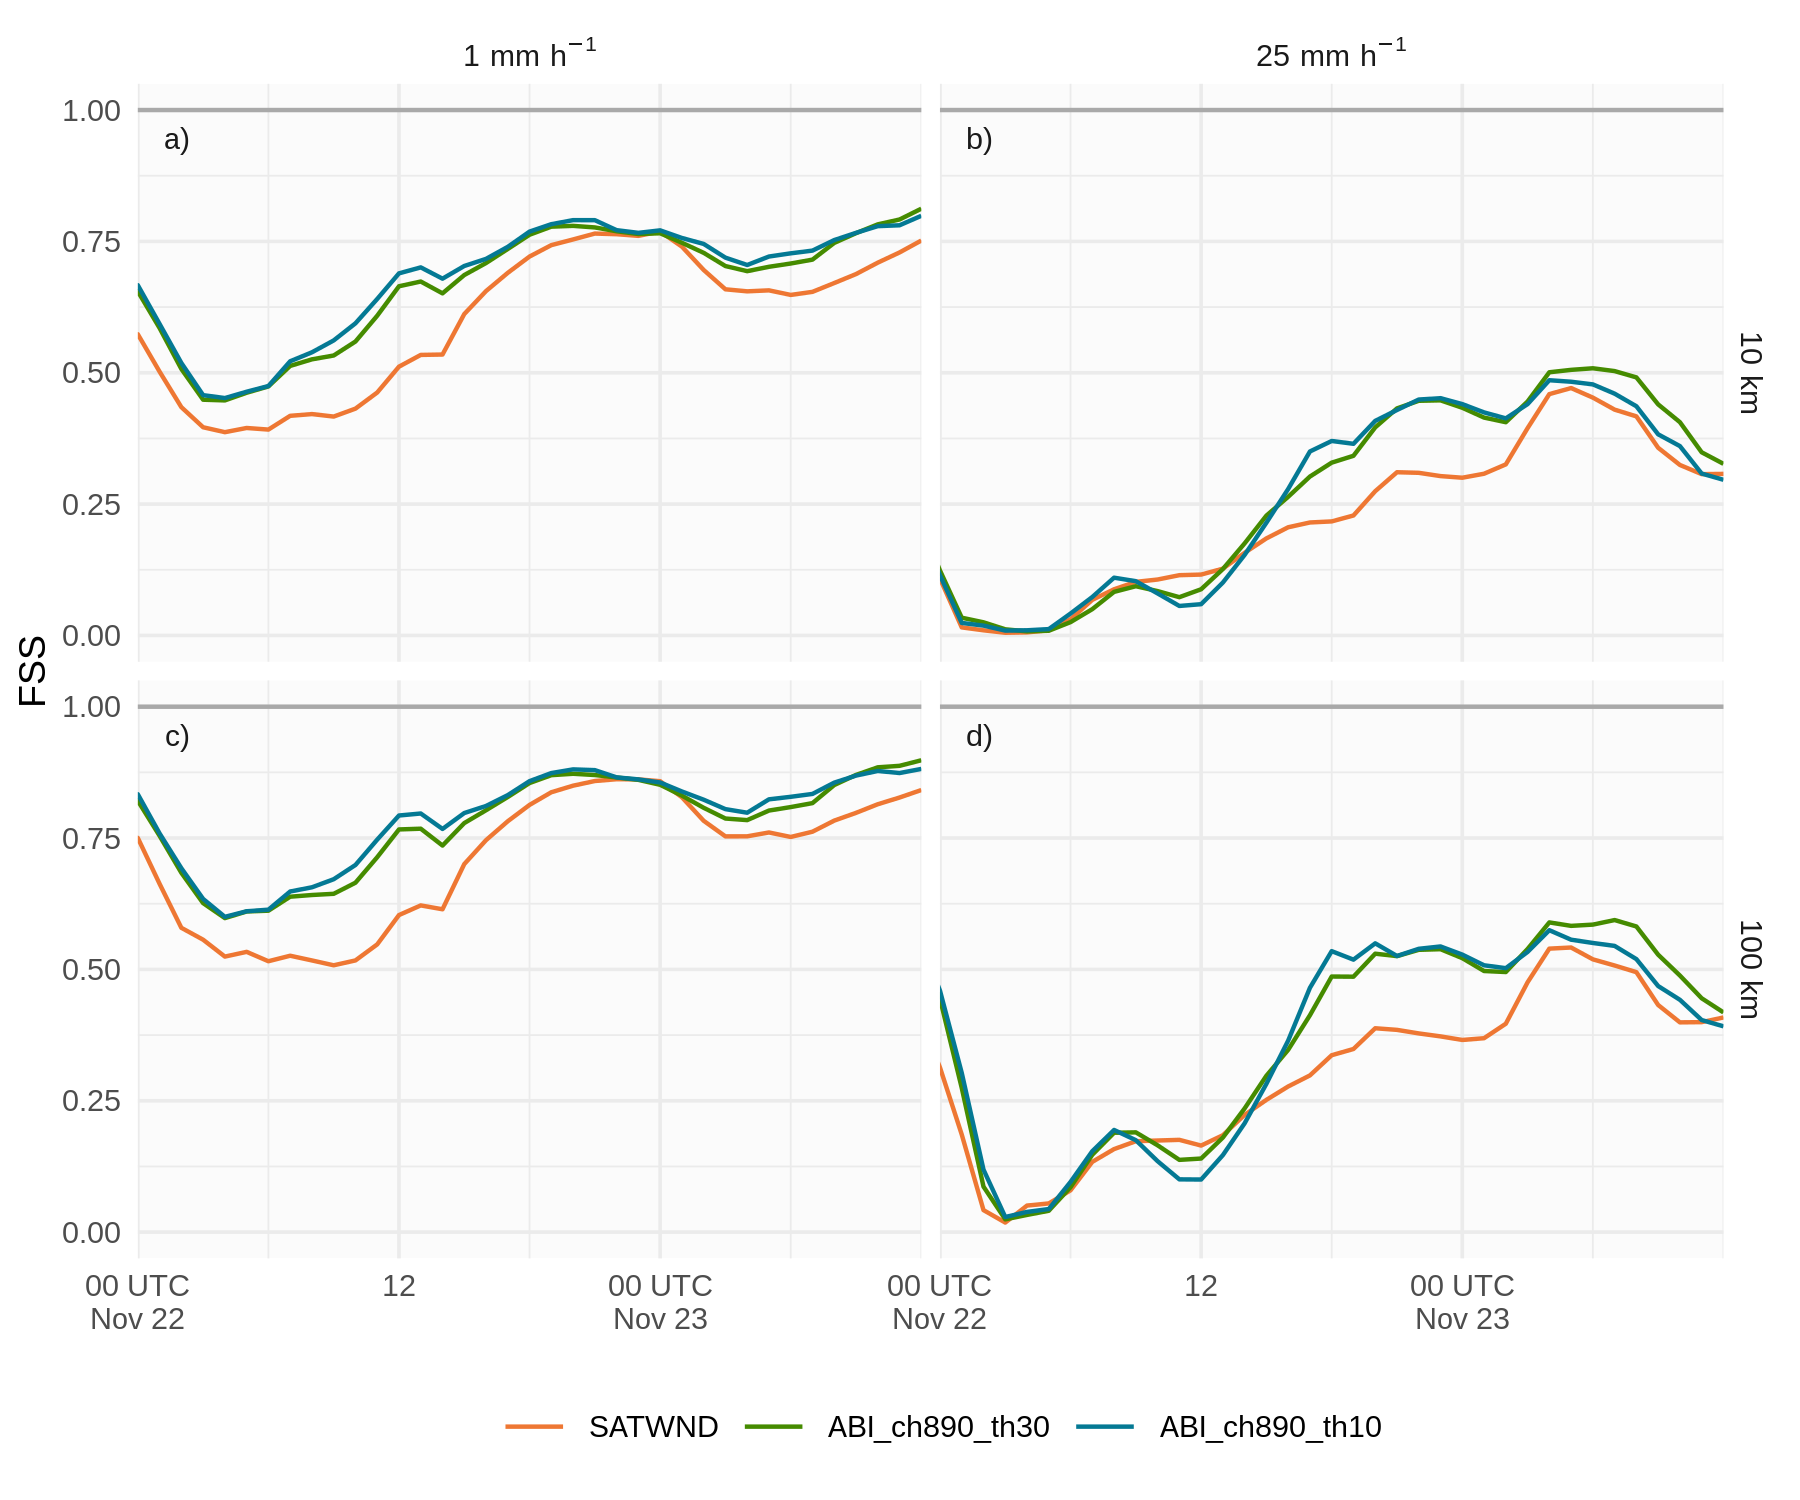
\includegraphics{thesis_files/figure-latex/thinning-fss-1} \caption{(ref:thinning-fss)}\label{fig:thinning-fss}
\end{figure}
Desde el punto de vista del FSS y para \(1 mm h^{-1}\) (Figura \ref{fig:thinning-fss}a y c) ABI\_ch890\_th10 tiene igual o mejor rendimiento que ABI\_ch890\_th30 pero ocurre lo contrario para el umbral de \(25 mm h^{-1}\) (Figura \ref{fig:thinning-fss}b y d). Si bien las diferencias de FSS entre los experimentos de thinning son muy pequeñas, en el caso del área cubierta por precipitación y otros análisis no mostrados, resalta la necesidad de utilizar un thinning cercano a la resolución del modelo. Por esta razón la configuración de thinning a utilizar en los experimentos posteriores será de 10 km.

\hypertarget{comparaciuxf3n-del-impacto-de-goes-16-versus-satuxe9lites-polares}{%
\subsection{Comparación del impacto de GOES-16 versus satélites polares}\label{comparaciuxf3n-del-impacto-de-goes-16-versus-satuxe9lites-polares}}

\hypertarget{analisis}{%
\subsubsection{Analisis}\label{analisis}}


\begin{figure}

{\centering 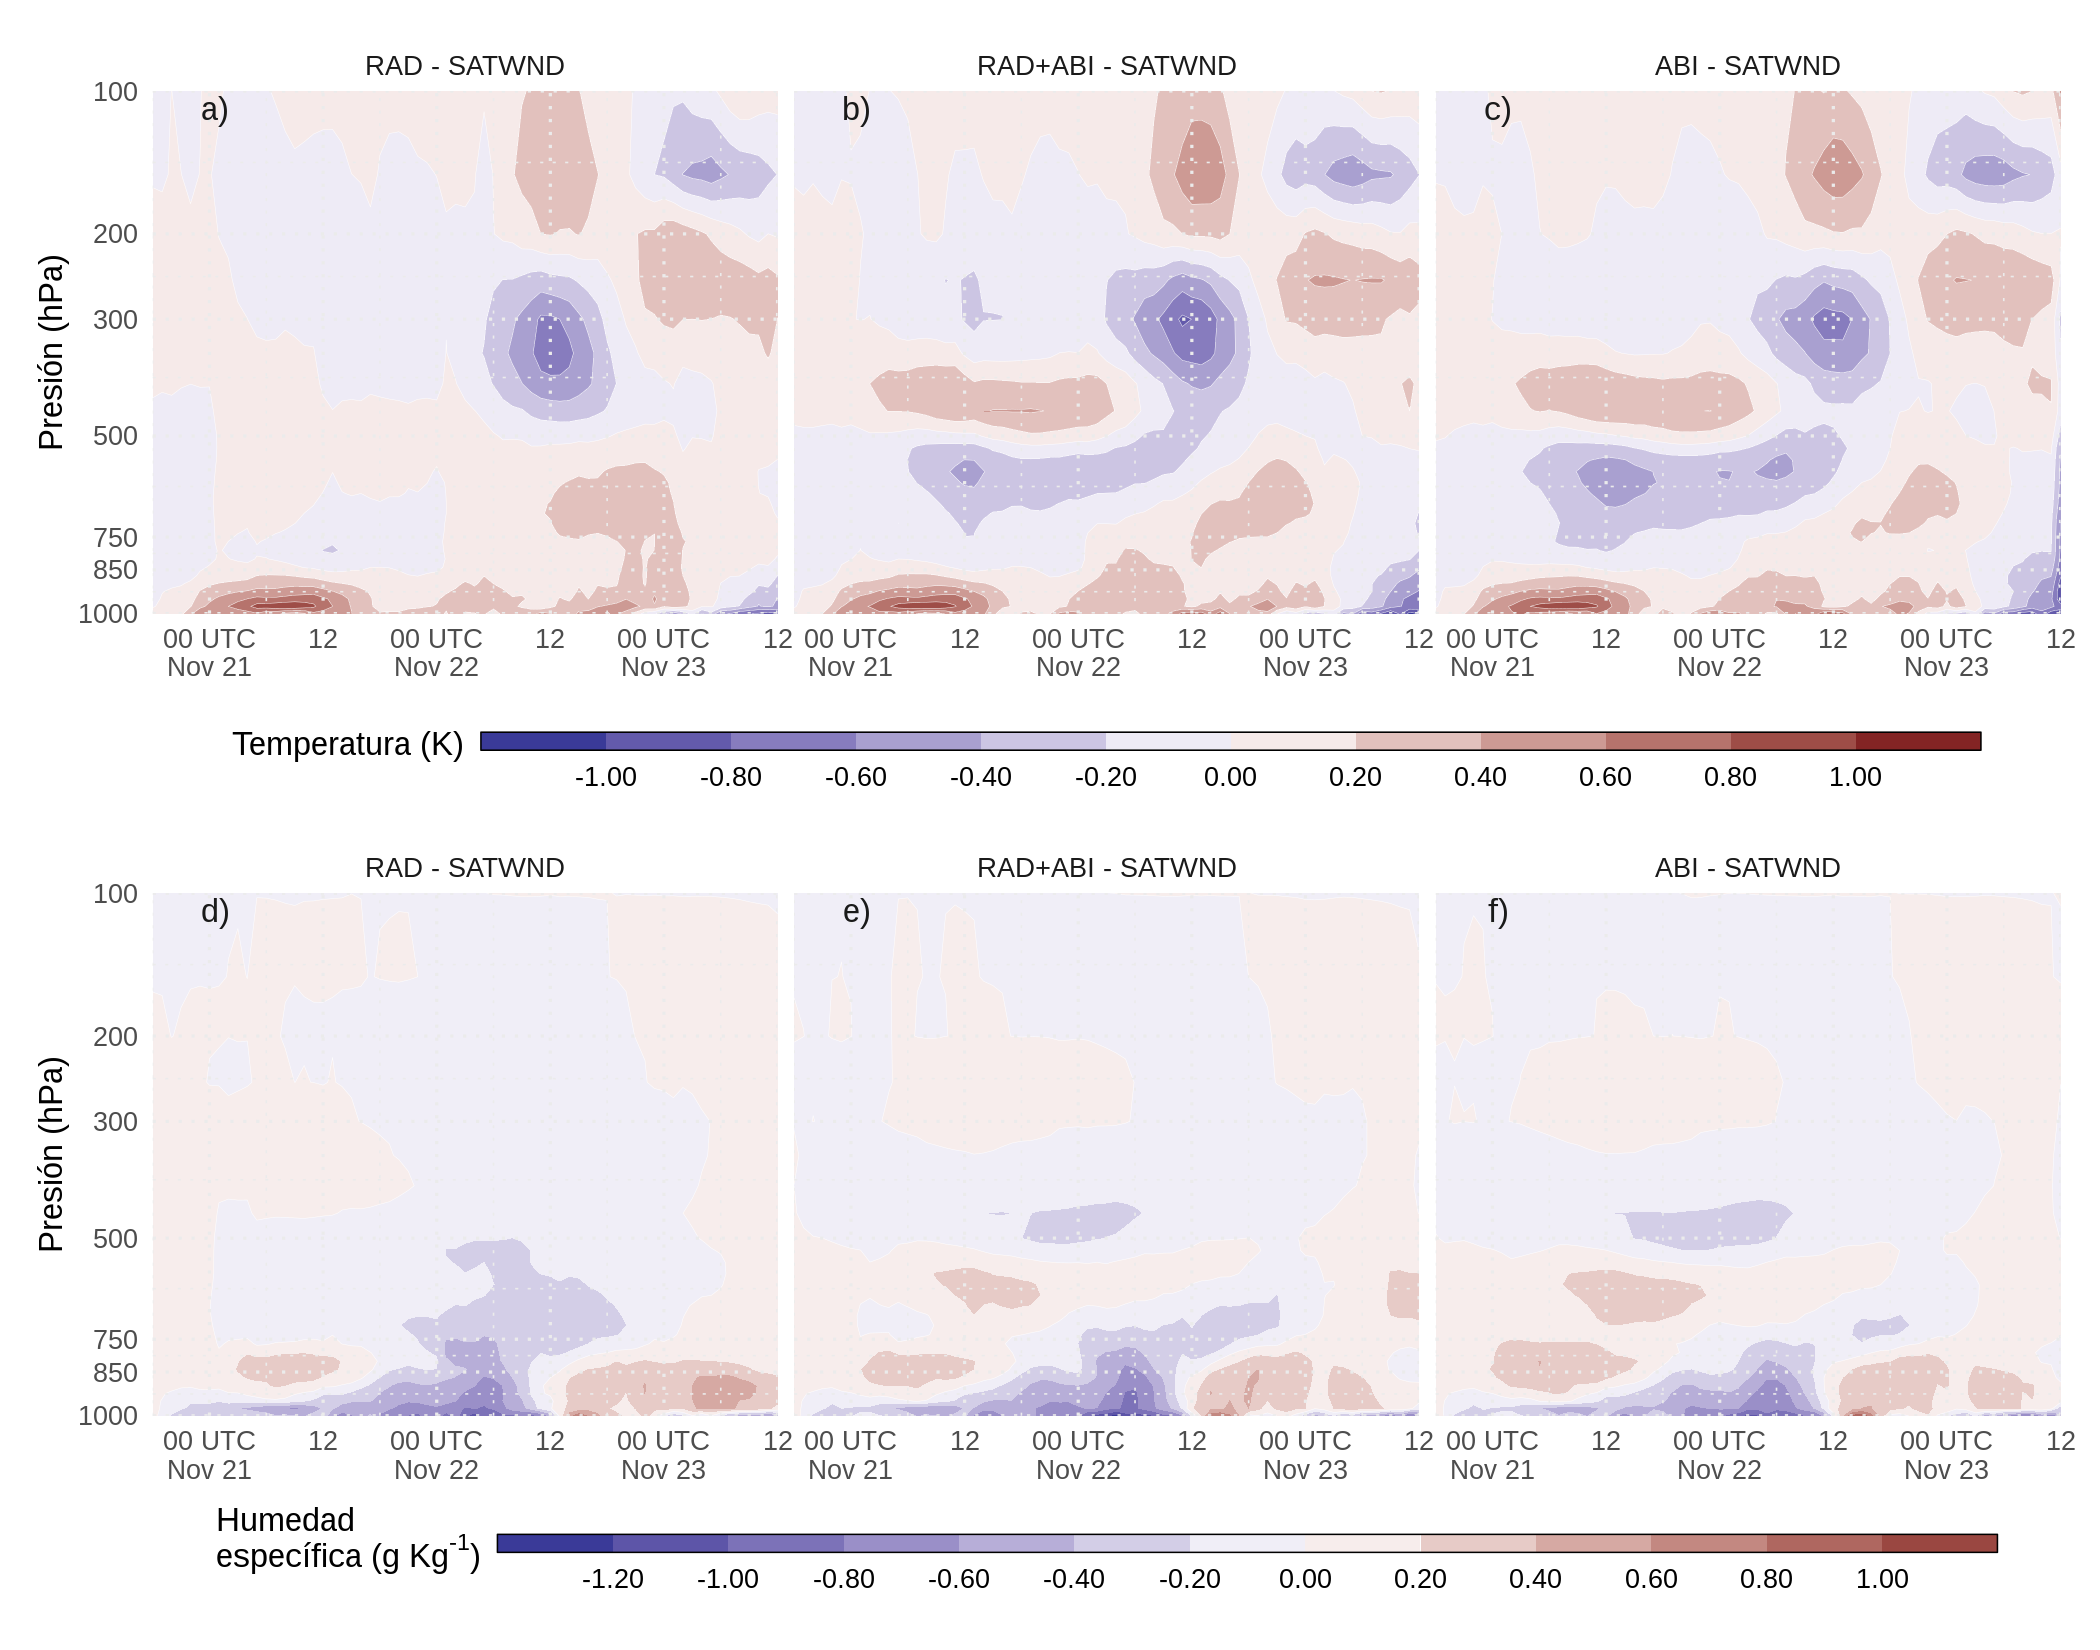
\includegraphics{thesis_files/figure-latex/TQ-diff-abi-1} 

}

\caption{Diferencia entre la media del ensamble de los análisis a) y d) RAD-SATWND, b) y e) RAD+ABI-SATWND, y c) y f) ABI-SATWND para los perfiles verticales espacialmente promediados de la temperatura (a, b y c, en \(K\)) y la humedad específica (d, e y f en \(g\ kg^{-1}\)) calculados sobre el dominio interior (recuadro rojo en la Figura \ref{fig:dominio}a) para cada ciclo de análisis.}\label{fig:TQ-diff-abi}
\end{figure}

\begin{figure}

{\centering 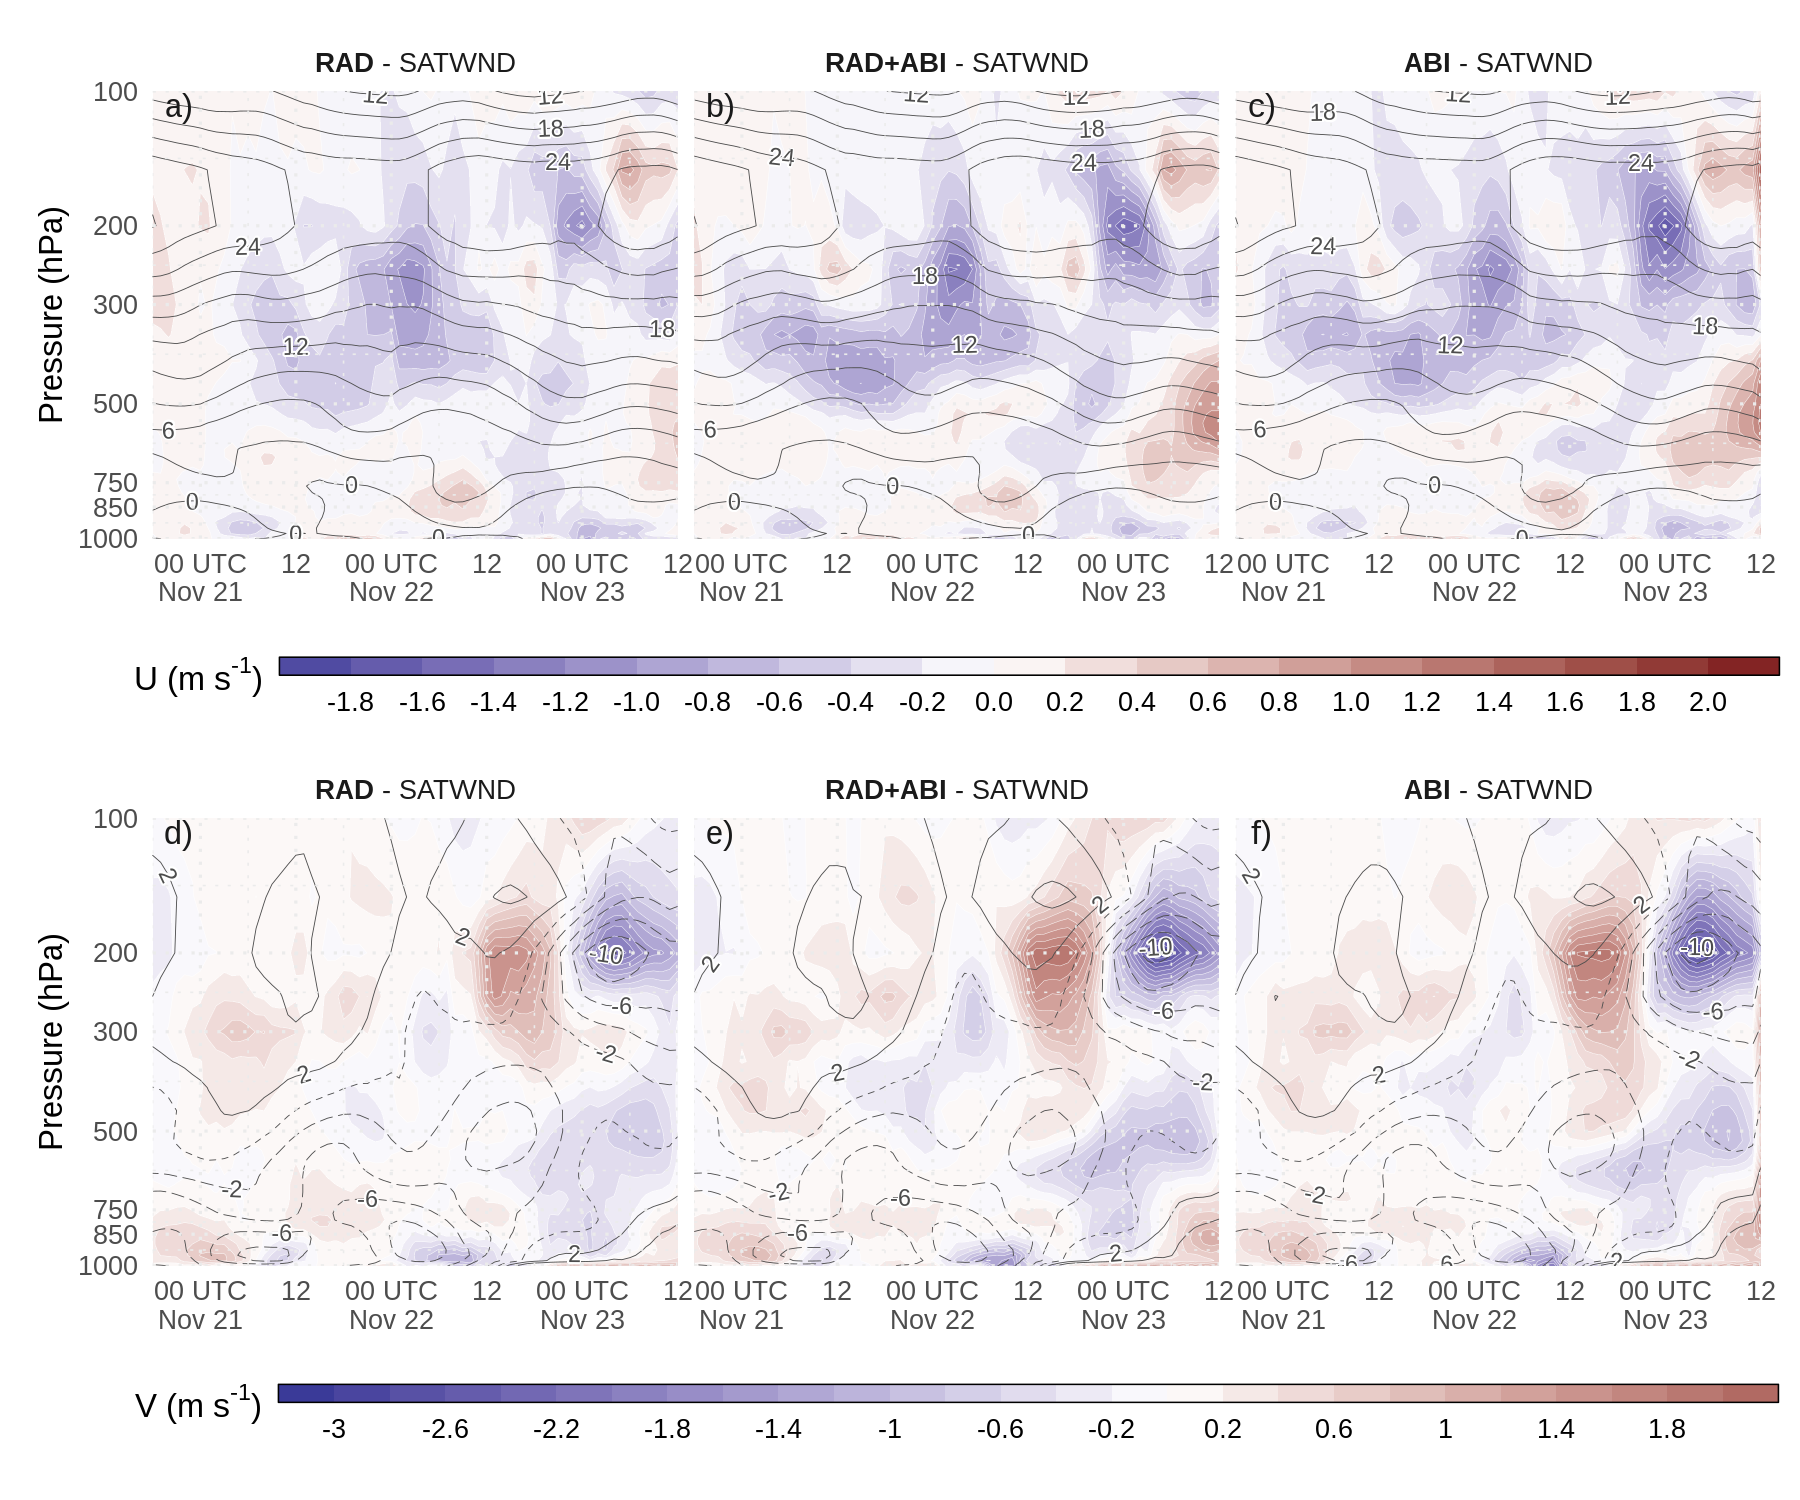
\includegraphics{thesis_files/figure-latex/UV-diff-abi-1} 

}

\caption{Diferencia entre la media del ensamble de los análisis a) y d) RAD-SATWND, b) y e) RAD+ABI-SATWND, y c) y f) ABI-SATWND para los perfiles verticales espacialmente promediados del viento zonal (a, b y c, en \(K\)) y viento meridional (d, e y f en \(g\ kg^{-1}\)) calculados sobre el dominio interior (recuadro rojo en la Figura \ref{fig:dominio}a) para cada ciclo de análisis. Los contornos negros corresponden al viento zonal y meridional para (a,d) RAD, (b,e) RAD+ABI, y (c,f) ABI ya que son los experimentos tienen más observaciones asimiladas en cada panel.}\label{fig:UV-diff-abi}
\end{figure}

\begin{figure}

{\centering 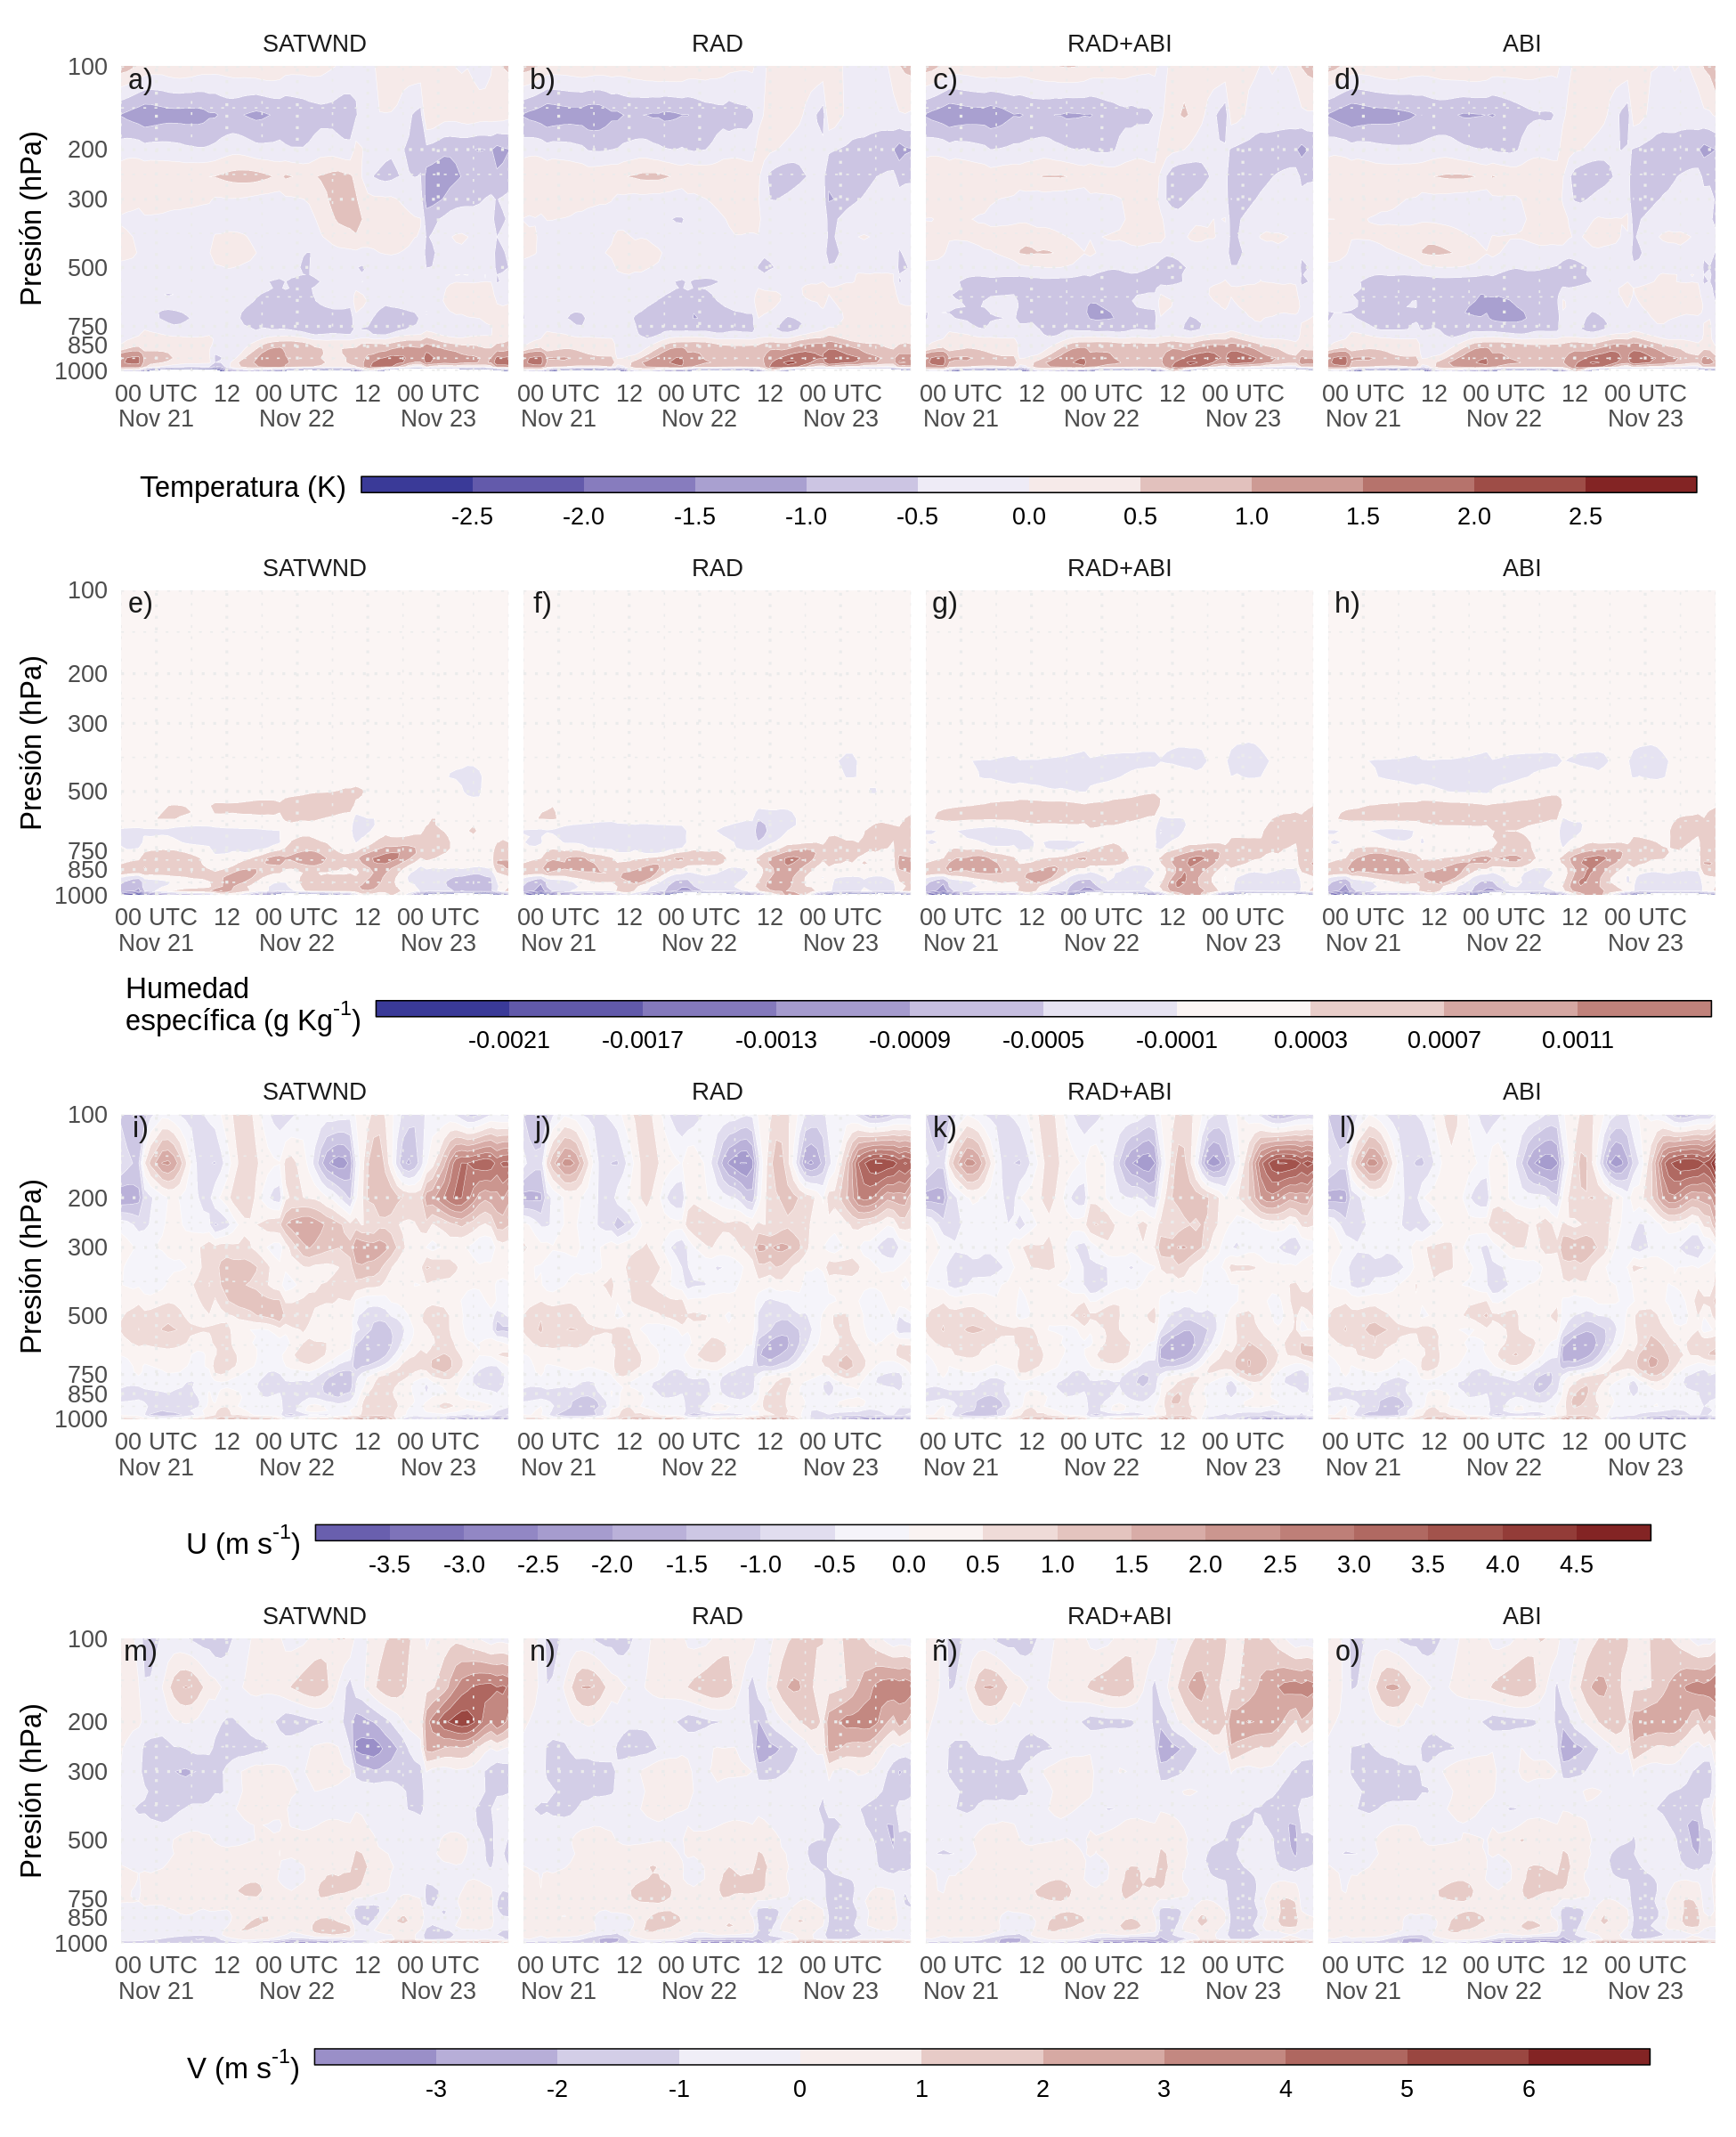
\includegraphics{thesis_files/figure-latex/era5-abi-1} 

}

\caption{Diferencia entre la media del ensamble del análisis de cada experimento y el ERA5 para los perfiles verticales espacialmente promediados de la temperatura del aire (K, a--d), la humedad específica (\(g\ Kg^{-1}\), e--h) y el viento meridional (\(m\ s^{-1}\), i--l) calculados sobre el dominio interior (recuadro rojo en la Figura \ref{fig:dominio}a) para cada ciclo de análisis.}\label{fig:era5-abi}
\end{figure}

\begin{figure}

{\centering 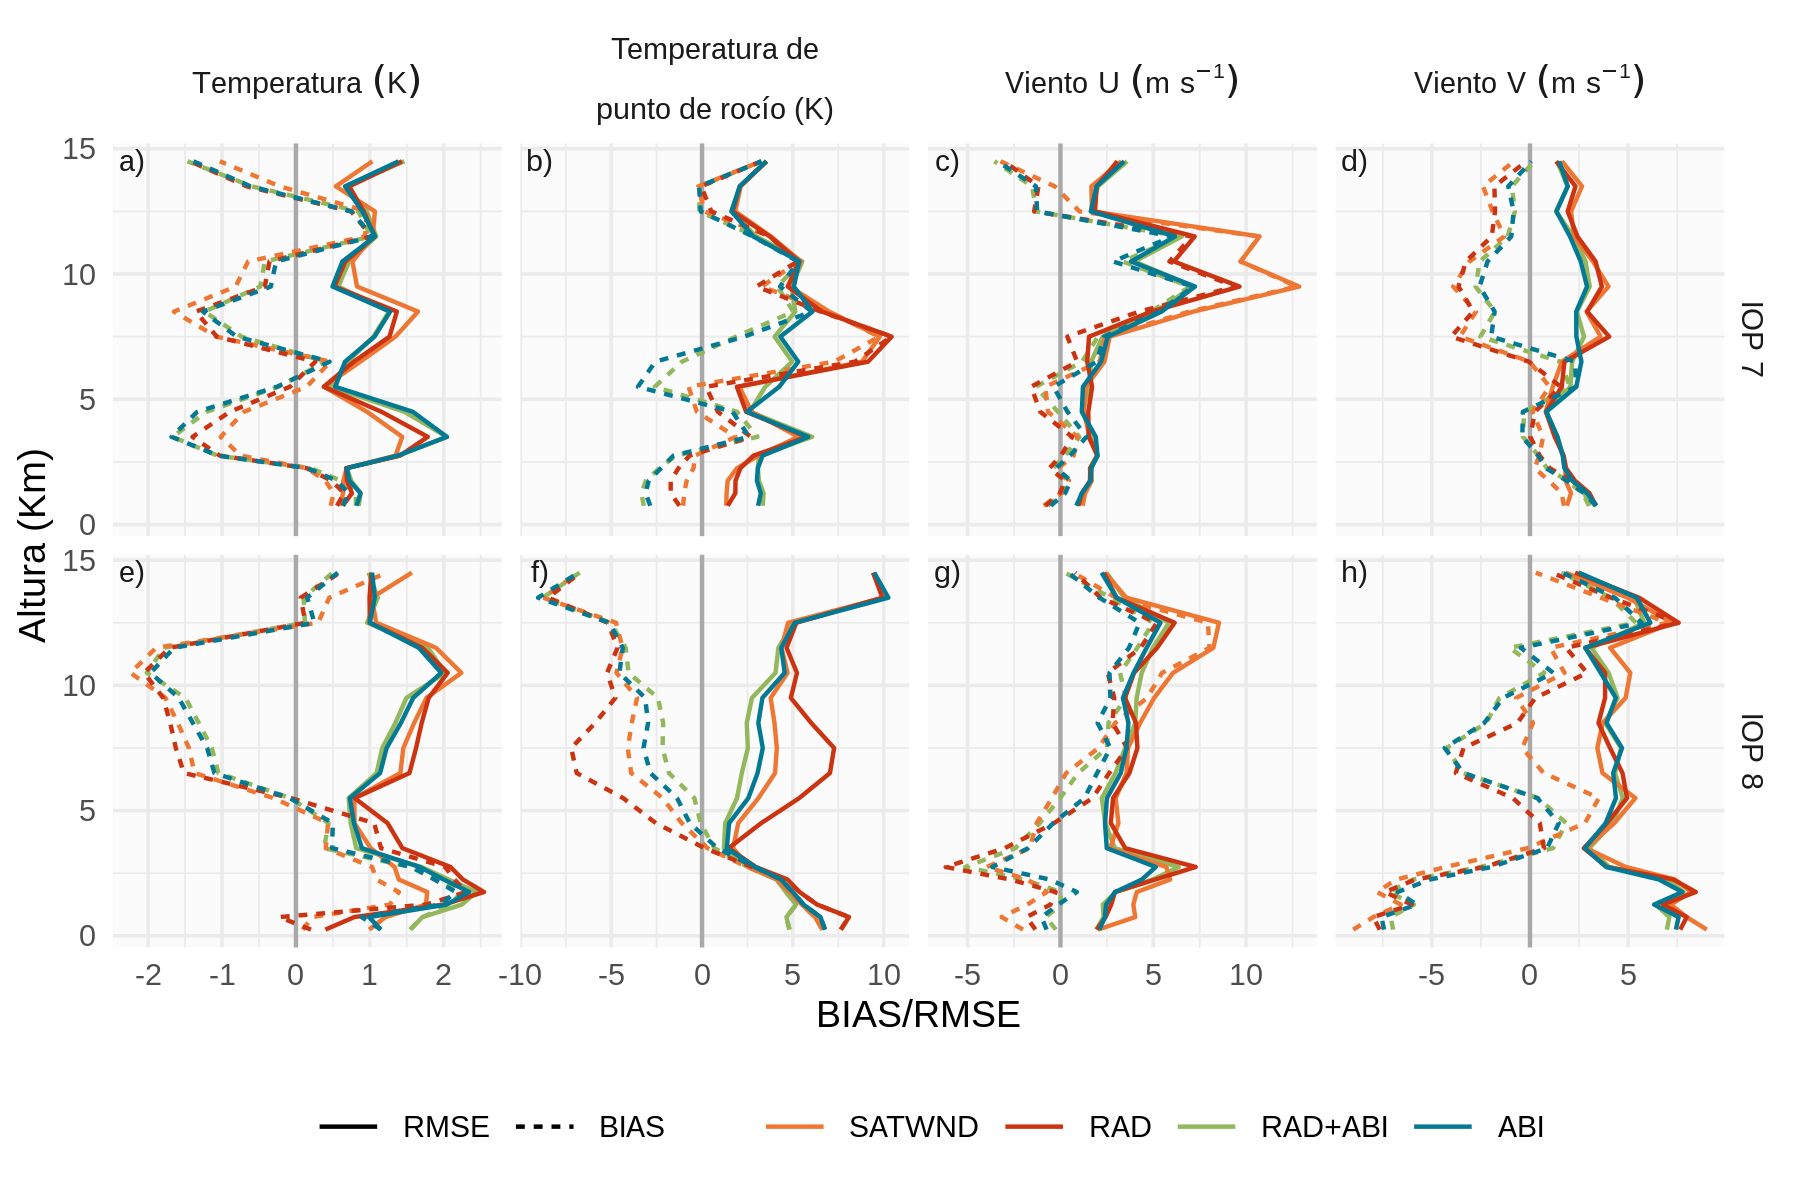
\includegraphics{thesis_files/figure-latex/sondeos-abi-1} 

}

\caption{RMSE (línea sólida) y Bias (línea discontinua) de a) la temperatura (\(K\)), b) la temperatura del punto de rocío (\(K\)), c) el viento u (\(m\ s^{-1}\)) y d) el viento v (\(m\ s^{-1}\)) calculados comparando el análisis de cada experimento con los sondeos de RELAMPAGO durante el IOP 7 y el IOP 8. La línea naranja corresponde a SATWND, la línea roja a RAD, RAD+ABI se representa con una línea verde y ABI con una línea turueza.}\label{fig:sondeos-abi}
\end{figure}
\begin{figure}
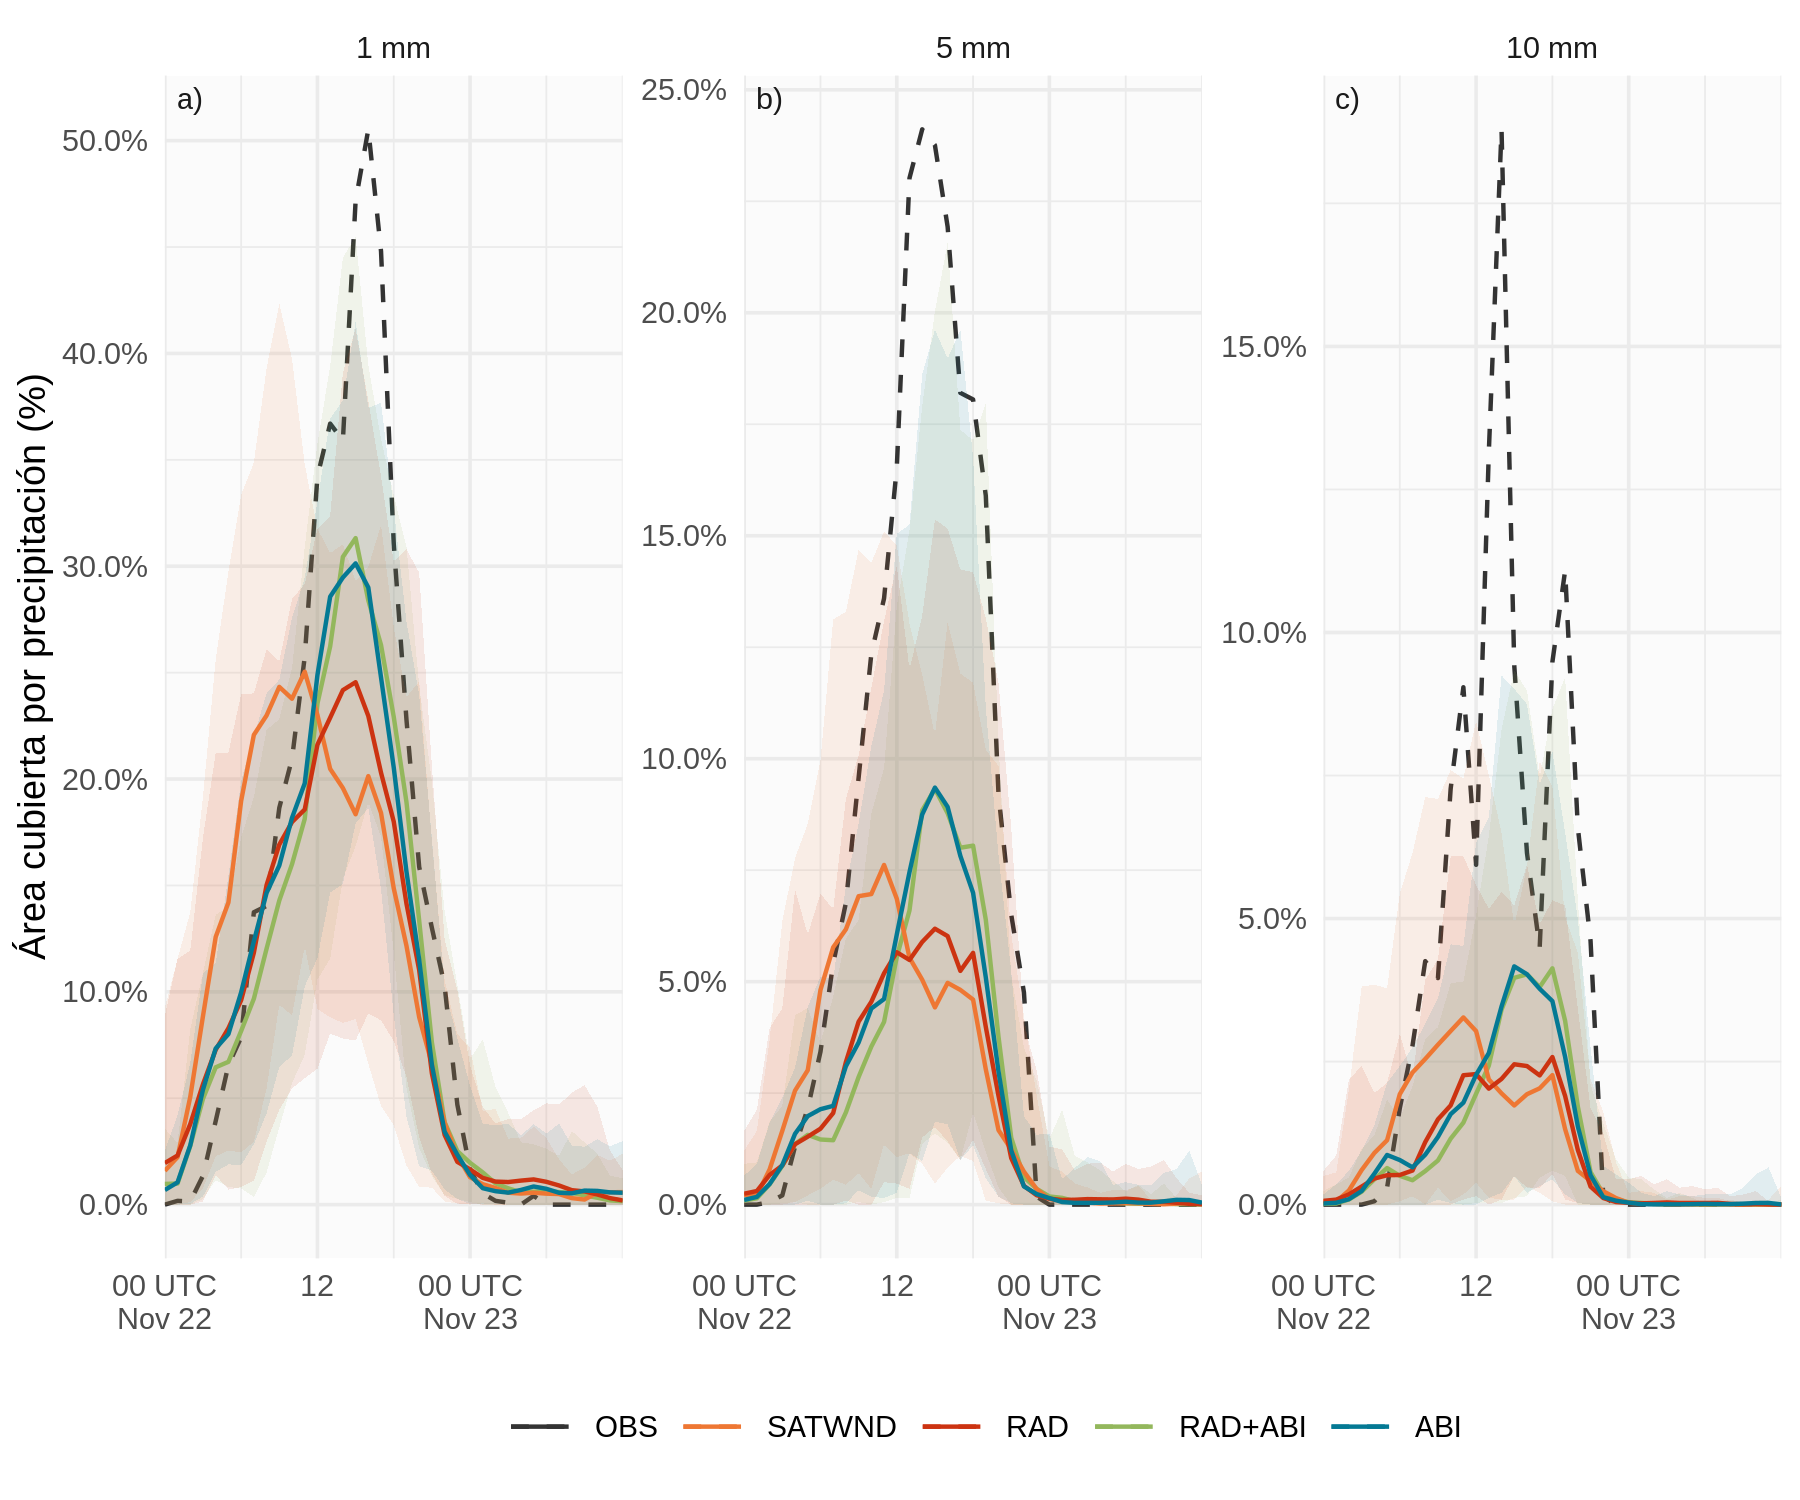
\includegraphics{thesis_files/figure-latex/area-abi-1} \caption{Porcentaje de área cubierta por precipitación a 1 hora superior a a) \(1 mmh^{-1}\), b) \(5 mmh^{-1}\) y c) \(10 mmh^{-1}\) a lo largo del tiempo para el campo preliminar de los experimentos SATWND (línea naranja), ABI\_ch890\_th30 (línea verde), ABI\_ch90\_th30 (línea violeta) y ABI\_ch0\_th30 (línea celeste) entre las 00 UTC del 22 de noviembre y las 12 UTC del 23 de noviembre en el dominio de verificación (cuadro rojo en la Figura \ref{fig:dominio}a). En sombreado y para cada experimento se muestra el área máxima y mínima estimada por el ensamble del análisis. En línea continua negra se muetra la estimación de IMERG.}\label{fig:area-abi}
\end{figure}
\begin{figure}
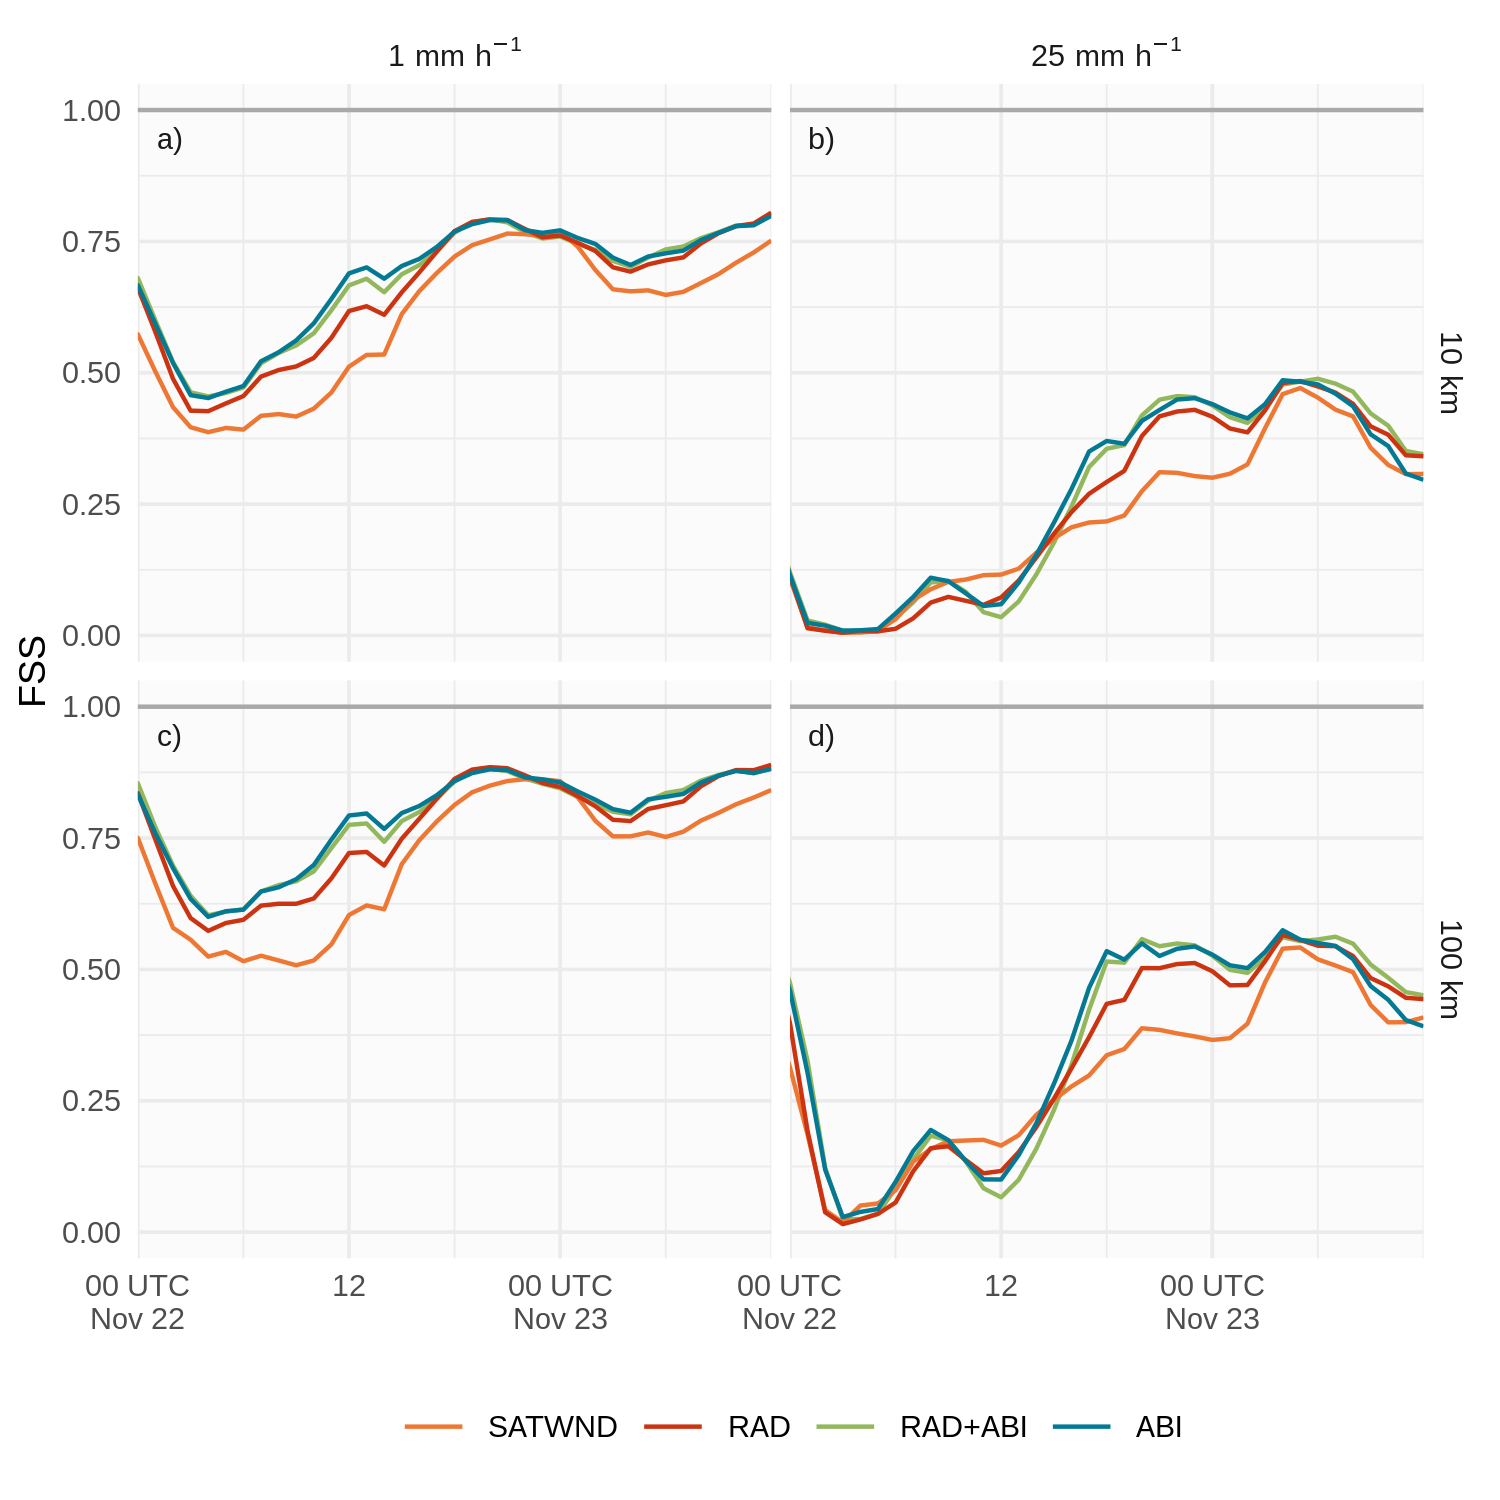
\includegraphics{thesis_files/figure-latex/fss-abi-1} \caption{(ref:fss-abi)}\label{fig:fss-abi}
\end{figure}
\hypertarget{pronuxf3sticos-determinuxedsticos}{%
\subsubsection{Pronósticos determinísticos}\label{pronuxf3sticos-determinuxedsticos}}

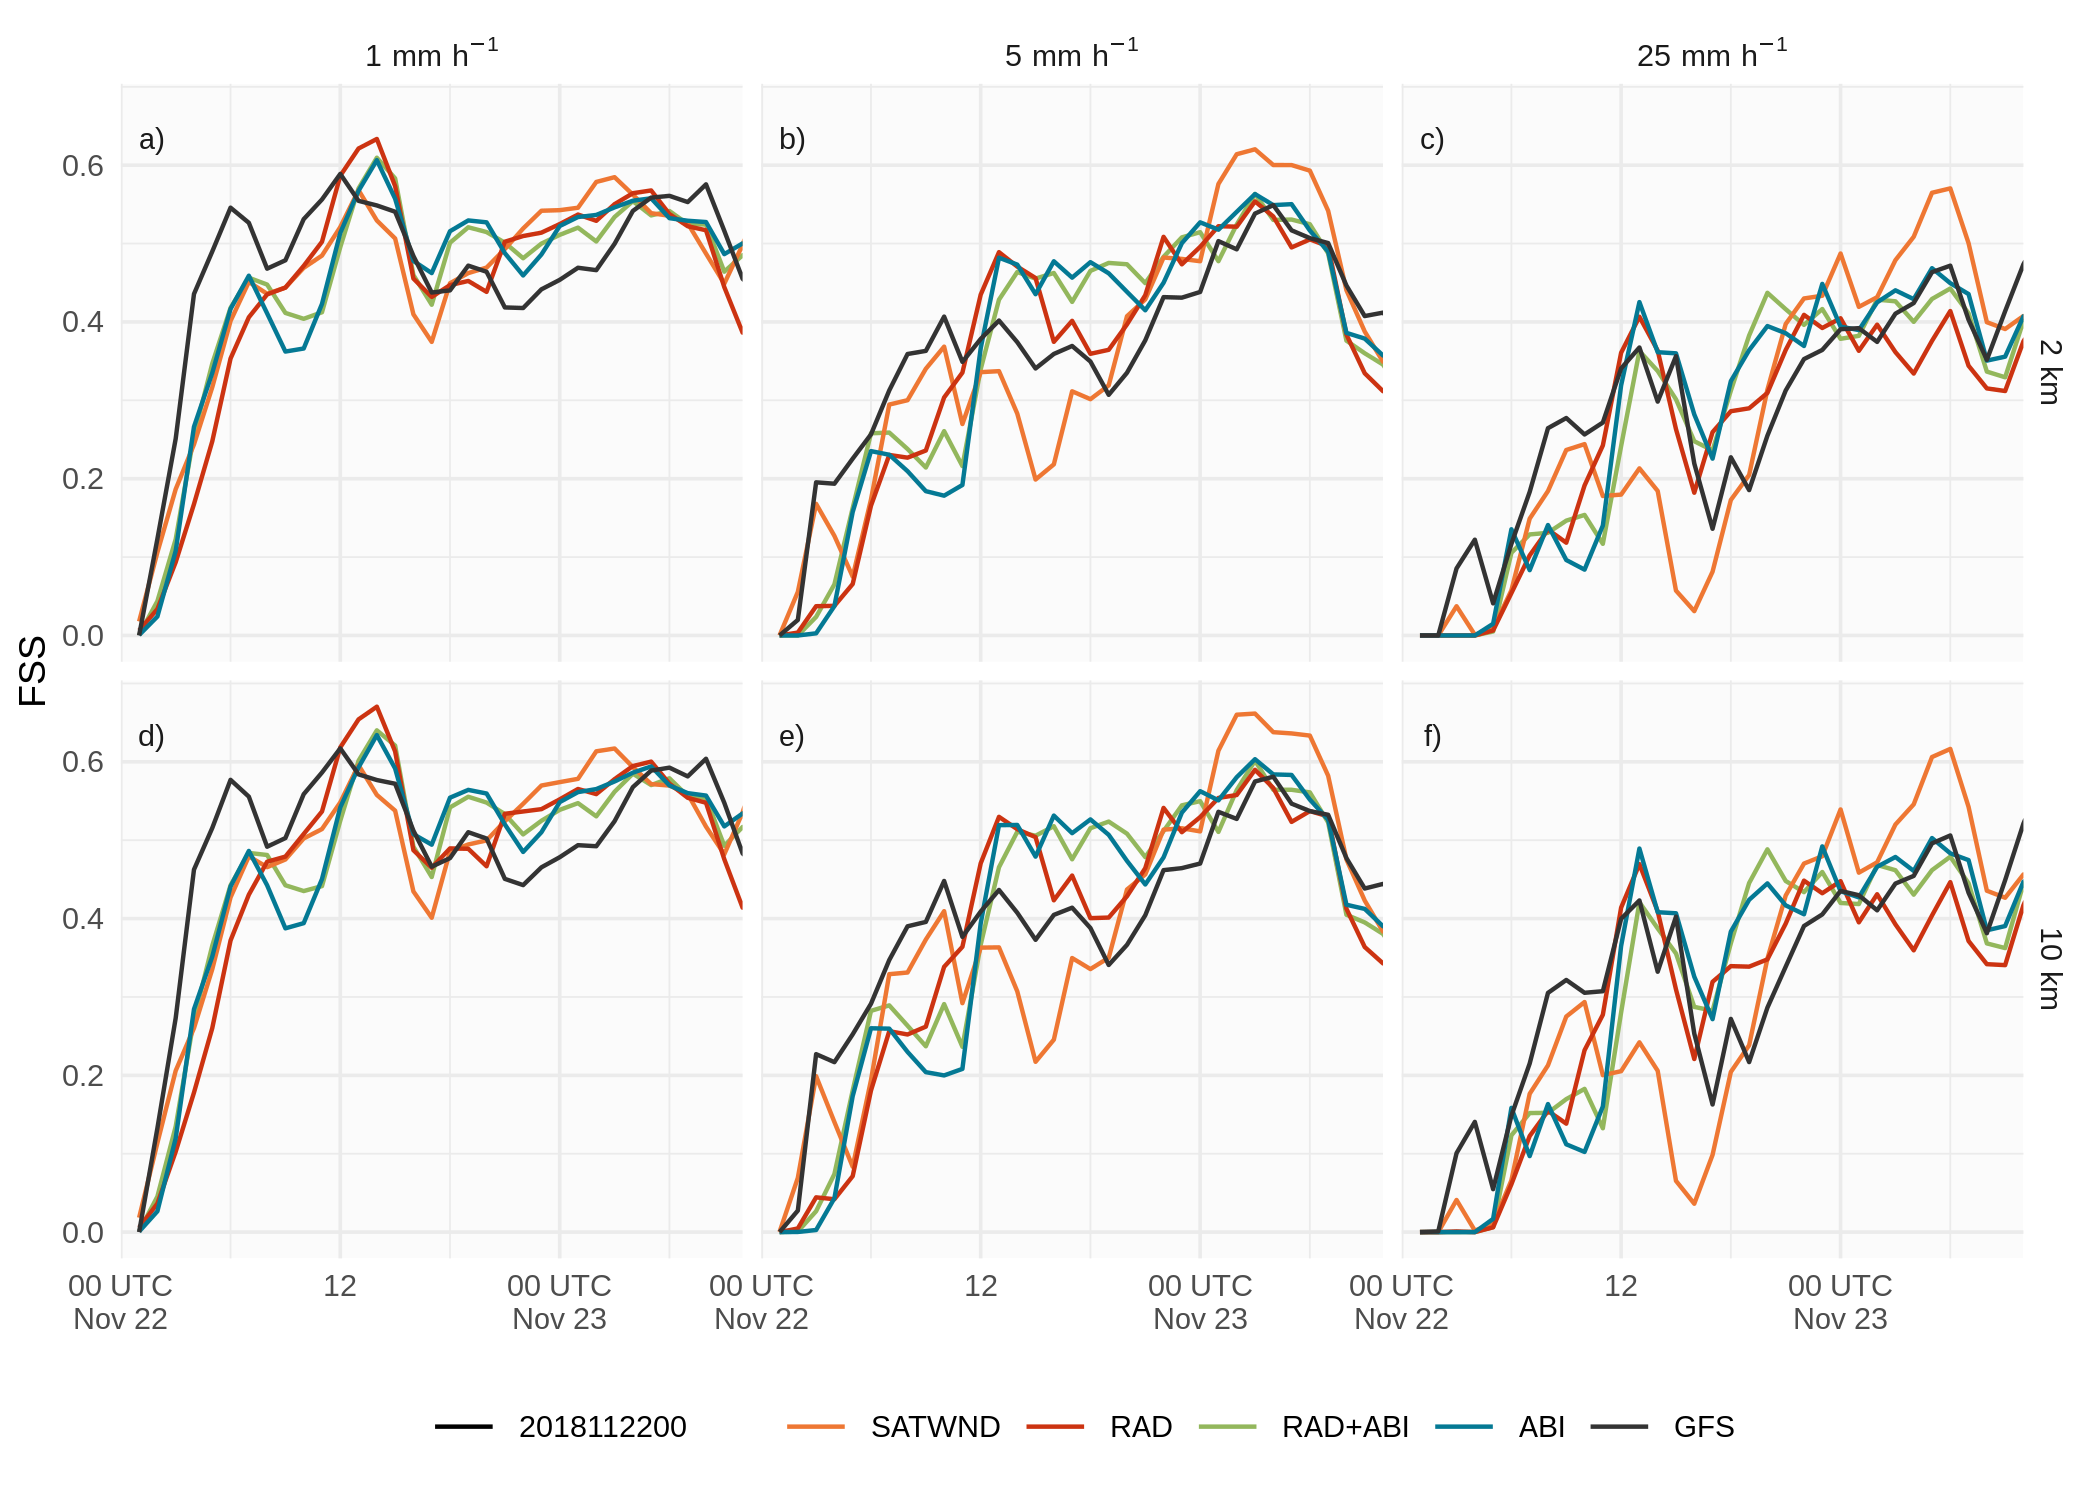
\includegraphics{thesis_files/figure-latex/unnamed-chunk-2-1}

\includegraphics{thesis_files/figure-latex/unnamed-chunk-3-1}

\hypertarget{conclusiones-2}{%
\section{Conclusiones}\label{conclusiones-2}}

\hypertarget{conclusiones-generales}{%
\chapter*{Conclusiones Generales}\label{conclusiones-generales}}
\addcontentsline{toc}{chapter}{Conclusiones Generales}

TBD

\appendix

\hypertarget{correcciuxf3n-del-bias-de-observaciones-de-satuxe9lite}{%
\chapter{Corrección del bias de observaciones de satélite}\label{correcciuxf3n-del-bias-de-observaciones-de-satuxe9lite}}

TBD

\backmatter

\hypertarget{referencias}{%
\chapter*{Referencias}\label{referencias}}
\addcontentsline{toc}{chapter}{Referencias}

\markboth{Referencias}{Referencias}

\noindent

\setlength{\parindent}{-0.20in}

\hypertarget{refs}{}
\leavevmode\hypertarget{ref-aksoy2010}{}%
Aksoy, A., Dowell, D.C., and Snyder, C., 2010. A Multicase Comparative Assessment of the Ensemble Kalman Filter for Assimilation of Radar Observations. Part II: Short-Range Ensemble Forecasts. Monthly Weather Review, 138, 4, 1273--1292.

\leavevmode\hypertarget{ref-allaire2019}{}%
Allaire, J., Horner, J., Xie, Y., Marti, V., and Porte, N., 2019. Markdown: Render markdown with the c library 'sundown'.

\leavevmode\hypertarget{ref-andersson1991}{}%
Andersson, E., Hollingsworth, A., Kelly, G., Lönnberg, P., Pailleux, J., and Zhang, Z., 1991. Global Observing System Experiments on Operational Statistical Retrievals of Satellite Sounding Data. Monthly Weather Review, 119, 8, 1851--1865.

\leavevmode\hypertarget{ref-bae2022}{}%
Bae, J.-H., and Min, K.-H., 2022. Forecast Characteristics of Radar Data Assimilation Based on the Scales of Precipitation Systems. Remote Sensing, 14, 3, 3, 605.

\leavevmode\hypertarget{ref-bao2015}{}%
Bao, Y., Xu, J., Powell Jr., A.M., Shao, M., Min, J., and Pan, Y., 2015. Impacts of AMSU-A, MHS and IASI data assimilation on temperature and humidity forecasts with GSI--WRF over the western United States. Atmospheric Measurement Techniques, 8, 10, 4231--4242.

\leavevmode\hypertarget{ref-baucemachado2017}{}%
Bauce Machado, V., gustavo goncalves, luis, Vendrasco, E., Sinhori, N., Herdies, D., Sapucci, L., Levien, C., Quadro, M., Rodrigues, T., and Cardoso, C. and others, 2017. Investigating the impacts of convective scale hazardous weather events in Santa Catarina State through the CPTEC/INPE local data assimilation system. In. Presented at the Seventh International WMO Symposium on Data Assimilation.

\leavevmode\hypertarget{ref-bauer2010}{}%
Bauer, P., Geer, A.J., Lopez, P., and Salmond, D., 2010. Direct 4D-Var assimilation of all-sky radiances. Part I: Implementation. Quarterly Journal of the Royal Meteorological Society, 136, 652, 1868--1885.

\leavevmode\hypertarget{ref-boukabara2011}{}%
Boukabara, S.-A., Garrett, K., Chen, W., Iturbide-Sanchez, F., Grassotti, C., Kongoli, C., Chen, R., Liu, Q., Yan, B., and Weng, F. and others, 2011. MiRS: An All-Weather 1DVAR Satellite Data Assimilation and Retrieval System. IEEE Transactions on Geoscience and Remote Sensing, 49, 9, 3249--3272. Presented at the IEEE Transactions on Geoscience and Remote Sensing.

\leavevmode\hypertarget{ref-campitelli2020}{}%
Campitelli, E., 2020, April. metR: Tools for Easier Analysis of Meteorological Fields.

\leavevmode\hypertarget{ref-candille2007}{}%
Candille, G., Côté, C., Houtekamer, P.L., and Pellerin, G., 2007. Verification of an Ensemble Prediction System against Observations. Monthly Weather Review, 135, 7, 2688--2699.

\leavevmode\hypertarget{ref-carrassi2018}{}%
Carrassi, A., Bocquet, M., Bertino, L., and Evensen, G., 2018. Data assimilation in the geosciences: An overview of methods, issues, and perspectives. WIREs Climate Change, 9, 5, e535.

\leavevmode\hypertarget{ref-casaretto2022}{}%
Casaretto, G., Dillon, M.E., Salio, P., Skabar, Y.G., Nesbitt, S.W., Schumacher, R.S., García, C.M., and Catalini, C., 2022. High-Resolution NWP Forecast Precipitation Comparison over Complex Terrain of the Sierras de Córdoba during RELAMPAGO-CACTI. Weather and Forecasting, 37, 2, 241--266.

\leavevmode\hypertarget{ref-chang2017}{}%
Chang, W., Jacques, D., Fillion, L., and Baek, S.-J., 2017. Assimilation of Hourly Surface Observations with the Canadian High-Resolution Ensemble Kalman Filter. Atmosphere-Ocean, 55, 4-5, 247--263.

\leavevmode\hypertarget{ref-chen2001}{}%
Chen, F., and Dudhia, J., 2001. Coupling an Advanced Land Surface--Hydrology Model with the Penn State--NCAR MM5 Modeling System. Part I: Model Implementation and Sensitivity. Monthly Weather Review, 129, 4, 569--585.

\leavevmode\hypertarget{ref-chen2015}{}%
Chen, Q., Fan, J., Hagos, S., Gustafson, W.I., and Berg, L.K., 2015. Roles of wind shear at different vertical levels: Cloud system organization and properties. Journal of Geophysical Research: Atmospheres, 120, 13, 6551--6574.

\leavevmode\hypertarget{ref-chen2016}{}%
Chen, X., Zhao, K., Sun, J., Zhou, B., and Lee, W.-C., 2016. Assimilating surface observations in a four-dimensional variational Doppler radar data assimilation system to improve the analysis and forecast of a squall line case. Advances in Atmospheric Sciences, 33, 10, 1106--1119.

\leavevmode\hypertarget{ref-cherubini2006}{}%
Cherubini, T., Businger, S., Velden, C., and Ogasawara, R., 2006. The Impact of Satellite-Derived Atmospheric Motion Vectors on Mesoscale Forecasts over Hawaii. Monthly Weather Review, 134, 7, 2009--2020.

\leavevmode\hypertarget{ref-clark2017}{}%
Clark, A.J., 2017. Generation of Ensemble Mean Precipitation Forecasts from Convection-Allowing Ensembles. Weather and Forecasting, 32, 4, 1569--1583.

\leavevmode\hypertarget{ref-clark2009}{}%
Clark, A.J., Gallus, W.A., Xue, M., and Kong, F., 2009. A Comparison of Precipitation Forecast Skill between Small Convection-Allowing and Large Convection-Parameterizing Ensembles. Weather and Forecasting, 24, 4, 1121--1140.

\leavevmode\hypertarget{ref-collard2007}{}%
Collard, A.D., 2007. Selection of IASI channels for use in numerical weather prediction: SELECTION OF IASI CHANNELS FOR NWP. Quarterly Journal of the Royal Meteorological Society, 133, 629, 1977--1991.

\leavevmode\hypertarget{ref-Cheyenne2019}{}%
Computational and Information Systems Laboratory, 2019. Cheyenne: HPE/SGI ICE XA System (University Community Computing). National Center for Atmospheric Research Boulder, CO.

\leavevmode\hypertarget{ref-crews2021}{}%
Crews, A., Blackwell, W.J., Leslie, R.V., Grant, M., Osaretin, I.A., DiLiberto, M., Milstein, A., Leroy, S., Gagnon, A., and Cahoy, K., 2021. Initial Radiance Validation of the Microsized Microwave Atmospheric Satellite-2A. IEEE Transactions on Geoscience and Remote Sensing, 59, 4, 2703--2714. Presented at the IEEE Transactions on Geoscience and Remote Sensing.

\leavevmode\hypertarget{ref-cutraro2021}{}%
Cutraro, F., Galligani, V.S., and Skabar, Y.G., 2021. Evaluation of synthetic satellite images computed from radiative transfer models over a region of South America using WRF and GOES-13/16 observations. Quarterly Journal of the Royal Meteorological Society, 147, 738, 2988--3003.

\leavevmode\hypertarget{ref-deelia2017}{}%
de Elía, R., Vidal, L., and Lohigorry, P., 2017. El SMN y la red argentina de radares meteorológicos (\url{http://hdl.handle.net/20.500.12160/625}).

\leavevmode\hypertarget{ref-dillon2017}{}%
Dillon, L.M.E., 2017. Asimilación de datos reales a escala regional en Argentina.

\leavevmode\hypertarget{ref-dillon2021}{}%
Dillon, M.E., Maldonado, P., Corrales, P., Skabar, Y.G., Ruiz, J., Sacco, M., Cutraro, F., Mingari, L., Matsudo, C., and Vidal, L. and others, 2021. A rapid refresh ensemble based data assimilation and forecast system for the RELAMPAGO field campaign. Atmospheric Research, 105858.

\leavevmode\hypertarget{ref-dowle2020}{}%
Dowle, M., and Srinivasan, A., 2020, July. Data.Table: Extension of 'data.frame'.

\leavevmode\hypertarget{ref-sondeos}{}%
Earth Observing Laboratory, U. -, 2020. Multi-network composite highest resolution radiosonde data. Version 1.3. UCAR/NCAR - earth observing laboratory.

\leavevmode\hypertarget{ref-english2000}{}%
English, S.J., Renshaw, R.J., Dibben, P.C., Smith, A.J., Rayer, P.J., Poulsen, C., Saunders, F.W., and Eyre, J.R., 2000. A comparison of the impact of TOVS arid ATOVS satellite sounding data on the accuracy of numerical weather forecasts. Quarterly Journal of the Royal Meteorological Society, 126, 569, 2911--2931.

\leavevmode\hypertarget{ref-evensen2009}{}%
Evensen, G., 2009. Data Assimilation, Springer,

\leavevmode\hypertarget{ref-eyre2020}{}%
Eyre, J.R., English, S.J., and Forsythe, M., 2020. Assimilation of satellite data in numerical weather prediction. Part I: The early years. Quarterly Journal of the Royal Meteorological Society, 146, 726, 49--68.

\leavevmode\hypertarget{ref-eyre2022}{}%
Eyre, J.R., Bell, W., Cotton, J., English, S.J., Forsythe, M., Healy, S.B., and Pavelin, E.G., 2022. Assimilation of satellite data in numerical weather prediction. Part II: Recent years. Quarterly Journal of the Royal Meteorological Society, 148, 743, 521--556.

\leavevmode\hypertarget{ref-ferreira2017}{}%
Ferreira, R.C., Herdies, D.L., Vendrasco, É.P., Beneti, C.A.A., and Biscaro, T.S., 2017. Impacto da Assimilação de Dados de Radar em Sistemas Convectivos de Mesoescala: Um Estudo de Caso. Revista Brasileira de Meteorologia, 32, 3, 447--458.

\leavevmode\hypertarget{ref-ferreira2020}{}%
Ferreira, R.C., Alves Júnior, M.P., Vendrasco, éder P., Aravéquia, J.A., Nolasco Junior, L.R., Biscaro, T.S., Ferreira, R.C., Alves Júnior, M.P., Vendrasco, éder P., and Aravéquia, J.A. and others, 2020. The Impact of Microphysics Parameterization on Precipitation Forecast Using Radar Data Assimilation. Revista Brasileira de Meteorologia, 35, 1, 123--134.

\leavevmode\hypertarget{ref-gao2015}{}%
Gao, F., Huang, X.-Y., Jacobs, N.A., and Wang, H., 2015. Assimilation of wind speed and direction observations: Results from real observation experiments. Tellus A: Dynamic Meteorology and Oceanography, 67, 1, 27132.

\leavevmode\hypertarget{ref-garcia2019}{}%
Garcia, F., Ruiz, J., Salio, P., Bechis, H., and Nesbitt, S., 2019. Argentina mesonet data. Version 1.1. UCAR/NCAR - earth observing laboratory.

\leavevmode\hypertarget{ref-garciaskabar1997}{}%
García Skabar, Y., 1997. Análisis objetivo regional para inicializar un modelo de diez niveles en forma operativa. Tesis de licenciatura en ciencias de la atmósfera.

\leavevmode\hypertarget{ref-gasperoni2018}{}%
Gasperoni, N.A., Wang, X., Brewster, K.A., and Carr, F.H., 2018. Assessing Impacts of the High-Frequency Assimilation of Surface Observations for the Forecast of Convection Initiation on 3 April 2014 within the Dallas--Fort Worth Test Bed. Monthly Weather Review, 146, 11, 3845--3872.

\leavevmode\hypertarget{ref-goncalvesdegoncalves2015}{}%
Goncalves de Goncalves, L.G., Sapucci, L., Vendrasco, E., de Mattos, J., Ferreira, C., Khamis, E., and Cruz, N., 2015. A rapid update data assimilation cycle over South America using 3DVar and EnKF. In The 20th International TOVS Study Conference (ITSC-20).

\leavevmode\hypertarget{ref-grell2013}{}%
Grell, G.A., and Freitas, S.R., 2013. A scale and aerosol aware stochastic convective parameterization for weather and air quality modeling. Atmospheric Chemistry and Physics Discussions, 13, 9, 23845--23893.

\leavevmode\hypertarget{ref-gustafsson2018}{}%
Gustafsson, N., Janjić, T., Schraff, C., Leuenberger, D., Weissmann, M., Reich, H., Brousseau, P., Montmerle, T., Wattrelot, E., and Bučánek, A. and others, 2018. Survey of data assimilation methods for convective‐scale numerical weather prediction at operational centres. Quarterly Journal of the Royal Meteorological Society, 144, 713, 1218--1256.

\leavevmode\hypertarget{ref-ha2014}{}%
Ha, S.-Y., and Snyder, C., 2014. Influence of Surface Observations in Mesoscale Data Assimilation Using an Ensemble Kalman Filter. Monthly Weather Review, 142, 4, 1489--1508.

\leavevmode\hypertarget{ref-han2006}{}%
Han, Y., Van Delst, P., Liu, Q., Weng, F., Yan, B., Treadon, R., and Derber, J., 2006. JCSDA Community Radiative Transfer Model (CRTM)---version 1 p. 40.

\leavevmode\hypertarget{ref-era5pressure}{}%
Hersbach, H., Bell, B., Berrisford, P., Biavati, G., Horányi, A., Muñoz Sabater, J., Nicolas, J., Peubey, C., Radu, R., and Rozum, I. and others, 2018. ERA5 hourly data on pressure levels from 1959 to present. Copernicus Climate Change Service (C3S) Climate Data Store (CDS), (Accessed on \(<\)08-08-2022\(>\)).

\leavevmode\hypertarget{ref-hohenegger2007}{}%
Hohenegger, C., and Schar, C., 2007. Atmospheric Predictability at Synoptic Versus Cloud-Resolving Scales. Bulletin of the American Meteorological Society, 88, 11, 1783--1794.

\leavevmode\hypertarget{ref-hong2006a}{}%
Hong, S.-Y., Noh, Y., and Dudhia, J., 2006. A New Vertical Diffusion Package with an Explicit Treatment of Entrainment Processes. Monthly Weather Review, 134, 9, 2318--2341.

\leavevmode\hypertarget{ref-hong2006}{}%
Hong, S.-Y., Kim, J.-H., Lim, J.-o., and Dudhia, J., 2006. The WRF Single Moment 6-Class Microphysics Scheme (WSM6). Journal of the Korean Meteorological Society, 42, 129--151.

\leavevmode\hypertarget{ref-hu2021}{}%
Hu, H., and Han, Y., 2021. Comparing the Thermal Structures of Tropical Cyclones Derived From Suomi NPP ATMS and FY-3D Microwave Sounders. IEEE Transactions on Geoscience and Remote Sensing, 59, 10, 8073--8083. Presented at the IEEE Transactions on Geoscience and Remote Sensing.

\leavevmode\hypertarget{ref-hu2019}{}%
Hu, H., Weng, F., Han, Y., and Duan, Y., 2019. Remote Sensing of Tropical Cyclone Thermal Structure from Satellite Microwave Sounding Instruments: Impacts of Background Profiles on Retrievals. Journal of Meteorological Research, 33, 1, 89--103.

\leavevmode\hypertarget{ref-hu2018}{}%
Hu, M., Ge, G., Zhou, C., Stark, D., Shao, H., Newman, K., Beck, J., and Zhang, X., 2018. Grid-point Statistical Interpolation (GSI) User's Guide Version 3.7, Developmental Testbed Center, p. 149.

\leavevmode\hypertarget{ref-huffman2018}{}%
Huffman, G., Bolvin, D., Braithwaite, D., Hsu, K., Joyce, R., Kidd, C., Nelkin, E., Sorooshian, S., Tan, J., and Xie, P., 2018. NASA Global Precipitation Measurement (GPM) Integrated Multi-satellitE Retrievals for GPM (IMERG), National Aeronautics and Space Administration (NASA), p. 35.

\leavevmode\hypertarget{ref-hunt2007}{}%
Hunt, B.R., Kostelich, E.J., and Szunyogh, I., 2007. Efficient data assimilation for spatiotemporal chaos: A local ensemble transform Kalman filter. Physica D: Nonlinear Phenomena, 230, 1-2, 112--126.

\leavevmode\hypertarget{ref-iacono2008}{}%
Iacono, M.J., Delamere, J.S., Mlawer, E.J., Shephard, M.W., Clough, S.A., and Collins, W.D., 2008. Radiative forcing by long-lived greenhouse gases: Calculations with the AER radiative transfer models. Journal of Geophysical Research, 113, D13, D13103.

\leavevmode\hypertarget{ref-iacovazzi2020}{}%
Iacovazzi, R., Lin, L., Sun, N., and Liu, Q., 2020. NOAA Operational Microwave Sounding Radiometer Data Quality Monitoring and Anomaly Assessment Using COSMIC GNSS Radio-Occultation Soundings. Remote Sensing, 12, 5, 5, 828.

\leavevmode\hypertarget{ref-ismay2022}{}%
Ismay, C., and Solomon, N., 2022. Thesisdown: An updated r markdown thesis template using the bookdown package.

\leavevmode\hypertarget{ref-janjic1994}{}%
Janjić, Z.I., 1994. The Step-Mountain Eta Coordinate Model: Further Developments of the Convection, Viscous Sublayer, and Turbulence Closure Schemes. Monthly Weather Review, 122, 5, 927--945.

\leavevmode\hypertarget{ref-jones2013}{}%
Jones, T.A., Otkin, J.A., Stensrud, D.J., and Knopfmeier, K., 2013. Assimilation of Satellite Infrared Radiances and Doppler Radar Observations during a Cool Season Observing System Simulation Experiment. Monthly Weather Review, 141, 10, 3273--3299.

\leavevmode\hypertarget{ref-jones2014}{}%
---------, 2014. Forecast Evaluation of an Observing System Simulation Experiment Assimilating Both Radar and Satellite Data. Monthly Weather Review, 142, 1, 107--124.

\leavevmode\hypertarget{ref-jones2020}{}%
Jones, T.A., Skinner, P., Yussouf, N., Knopfmeier, K., Reinhart, A., Wang, X., Bedka, K., Smith, W., and Palikonda, R., 2020. Assimilation of GOES-16 Radiances and Retrievals into the Warn-on-Forecast System. Monthly Weather Review, 148, 5, 1829--1859.

\leavevmode\hypertarget{ref-kain2004}{}%
Kain, J.S., 2004. The Kain--Fritsch Convective Parameterization: An Update. JOURNAL OF APPLIED METEOROLOGY, 43, 12.

\leavevmode\hypertarget{ref-kalnay2002}{}%
Kalnay, E., 2002, November 6. Atmospheric Modeling, Data Assimilation and Predictability (\url{https://www.cambridge.org/highereducation/books/atmospheric-modeling-data-assimilation-and-predictability/C5FD207439132836E85027754CE9BC1A}).

\leavevmode\hypertarget{ref-kelly1978}{}%
Kelly, G.a.M., Mills, G.A., and Smith, W.L., 1978. Impact of Nimbus-6 Temperature Soundings on Australian Region Forecasts. Bulletin of the American Meteorological Society, 59, 4, 393--406.

\leavevmode\hypertarget{ref-kleist2009}{}%
Kleist, D.T., Parrish, D.F., Derber, J.C., Treadon, R., Wu, W.-S., and Lord, S., 2009. Introduction of the GSI into the NCEP Global Data Assimilation System. Weather and Forecasting, 24, 6, 1691--1705.

\leavevmode\hypertarget{ref-lee2019}{}%
Lee, J.-R., Li, J., Li, Z., Wang, P., and Li, J., 2019. ABI Water Vapor Radiance Assimilation in a Regional NWP Model by Accounting for the Surface Impact. Earth and Space Science, 6, 9, 1652--1666.

\leavevmode\hypertarget{ref-lim2014}{}%
Lim, A.H., Jung, J.A., Huang, H.-L.A., Ackerman, S.A., and Otkin, J.A., 2014. Assimilation of clear sky Atmospheric Infrared Sounder radiances in short-term regional forecasts using community models. Journal of Applied Remote Sensing, 8, 1, 083655.

\leavevmode\hypertarget{ref-lin2017a}{}%
Lin, H., Weygandt, S.S., Lim, A.H.N., Hu, M., Brown, J.M., and Benjamin, S.G., 2017. Radiance Preprocessing for Assimilation in the Hourly Updating Rapid Refresh Mesoscale Model: A Study Using AIRS Data. Weather and Forecasting, 32, 5, 1781--1800.

\leavevmode\hypertarget{ref-liu2019}{}%
Liu, H., Collard, A., Derber, J., Nebuda, S., and Jung, J.A., 2019. Evaluation of GOES-16 Clear-sky Radiance Data and Preliminary Assimilation Results at NCEP, 2 pags.

\leavevmode\hypertarget{ref-liu2008}{}%
Liu, Q., Weng, F., Han, Y., and van Delst, P., 2008. Community Radiative Transfer Model for Scattering Transfer and Applications. In IGARSS 2008 - 2008 IEEE International Geoscience and Remote Sensing Symposium Vol. 4, pp. IV--1193--IV--1196. Presented at the IGARSS 2008 - 2008 IEEE International Geoscience and Remote Sensing Symposium.

\leavevmode\hypertarget{ref-maejima2019}{}%
Maejima, Y., Miyoshi, T., Kunii, M., Seko, H., and Sato, K., 2019. Impact of Dense and Frequent Surface Observations on 1-Minute-Update Severe Rainstorm Prediction: A Simulation Study. Journal of the Meteorological Society of Japan. Ser. II, 97, 1, 253--273.

\leavevmode\hypertarget{ref-maldonado2021}{}%
Maldonado, P., Ruiz, J., and Saulo, C., 2021. Sensitivity to Initial and Boundary Perturbations in Convective-Scale Ensemble-Based Data Assimilation: Imperfect-Model OSSEs. SOLA, 17, 0, 96--102.

\leavevmode\hypertarget{ref-markowski2010}{}%
Markowski, P., and Richardson, Y., 2010. Organization of Isolated Convection. In Mesoscale Meteorology in Midlatitudes pp. 201--244.

\leavevmode\hypertarget{ref-matsudo2021}{}%
Matsudo, C., Salles, M.A., and García Skabar, Y., 2021. Verificación de los pronósticos del esquema determinístico del modelo WRF para el año 2020.

\leavevmode\hypertarget{ref-nakanishi2009}{}%
Nakanishi, M., and Niino, H., 2009. Development of an Improved Turbulence Closure Model for the Atmospheric Boundary Layer. Journal of the Meteorological Society of Japan, 87, 5, 895--912.

\leavevmode\hypertarget{ref-cisl_rda_ds084.1}{}%
National Centers for Environmental Prediction, National Weather Service, NOAA, U.S. Department of Commerce, 2015. NCEP GFS 0.25 degree global forecast grids historical archive.

\leavevmode\hypertarget{ref-necker2020}{}%
Necker, T., Geiss, S., Weissmann, M., Ruiz, J., Miyoshi, T., and Lien, G., 2020. A convective‐scale 1,000‐member ensemble simulation and potential applications. Quarterly Journal of the Royal Meteorological Society, 146, 728, 1423--1442.

\leavevmode\hypertarget{ref-nesbitt2021}{}%
Nesbitt, S.W., Salio, P.V., Ávila, E., Bitzer, P., Carey, L., Chandrasekar, V., Deierling, W., Dominguez, F., Dillon, M.E., and Garcia, C.M. and others, 2021. A storm safari in Subtropical South America: Proyecto RELAMPAGO. Bulletin of the American Meteorological Society, -1, aop, 1--64.

\leavevmode\hypertarget{ref-ohring1979}{}%
Ohring, G., 1979. Impact of Satellite Temperature Sounding Data on Weather Forecasts. Bulletin of the American Meteorological Society, 60, 10, 1142--1147.

\leavevmode\hypertarget{ref-orlanski1975}{}%
Orlanski, I., 1975. A Rational Subdivision of Scales for Atmospheric Processes. Bulletin of the American Meteorological Society, 56, 5, 527--530.

\leavevmode\hypertarget{ref-ouaraini2015}{}%
Ouaraini, R.E., Berre, L., Fischer, C., and Sayouty, E.H., 2015. Sensitivity of regional ensemble data assimilation spread to perturbations of lateral boundary conditions. Tellus A: Dynamic Meteorology and Oceanography, 67, 1, 28502.

\leavevmode\hypertarget{ref-patil2001}{}%
Patil, D.J., Hunt, B.R., Kalnay, E., Yorke, J.A., and Ott, E., 2001. Local Low Dimensionality of Atmospheric Dynamics. Physical Review Letters, 86, 26, 5878--5881.

\leavevmode\hypertarget{ref-pondeca2011}{}%
Pondeca, M.S.F.V.D., Manikin, G.S., DiMego, G., Benjamin, S.G., Parrish, D.F., Purser, R.J., Wu, W.-S., Horel, J.D., Myrick, D.T., and Lin, Y. and others, 2011. The Real-Time Mesoscale Analysis at NOAA's National Centers for Environmental Prediction: Current Status and Development. Weather and Forecasting, 26, 5, 593--612.

\leavevmode\hypertarget{ref-purser2003a}{}%
Purser, R.J., Wu, W.-S., Parrish, D.F., and Roberts, N.M., 2003a. Numerical Aspects of the Application of Recursive Filters to Variational Statistical Analysis. Part II: Spatially Inhomogeneous and Anisotropic General Covariances. Monthly Weather Review, 131, 8, 1536--1548.

\leavevmode\hypertarget{ref-purser2003}{}%
---------, 2003b. Numerical Aspects of the Application of Recursive Filters to Variational Statistical Analysis. Part I: Spatially Homogeneous and Isotropic Gaussian Covariances. Monthly Weather Review, 131, 8, 1524--1535.

\leavevmode\hypertarget{ref-rabier2002}{}%
Rabier, F., Fourrié, N., Chafäi, D., and Prunet, P., 2002. Channel selection methods for Infrared Atmospheric Sounding Interferometer radiances. Quarterly Journal of the Royal Meteorological Society, 128, 581, 1011--1027.

\leavevmode\hypertarget{ref-rcoreteam2020}{}%
R Core Team, 2020. R: A language and environment for statistical computing, R Foundation for Statistical Computing,

\leavevmode\hypertarget{ref-roberts2020}{}%
Roberts, B., Gallo, B.T., Jirak, I.L., Clark, A.J., Dowell, D.C., Wang, X., and Wang, Y., 2020. What Does a Convection-Allowing Ensemble of Opportunity Buy Us in Forecasting Thunderstorms? Weather and Forecasting, 35, 6, 2293--2316.

\leavevmode\hypertarget{ref-roberts2008}{}%
Roberts, N., 2008. Assessing the spatial and temporal variation in the skill of precipitation forecasts from an NWP model. Meteorological Applications, 15, 1, 163--169.

\leavevmode\hypertarget{ref-ruiz2010}{}%
Ruiz, J.J., Saulo, C., and Nogués-Paegle, J., 2010. WRF Model Sensitivity to Choice of Parameterization over South America: Validation against Surface Variables. Monthly Weather Review, 138, 8, 3342--3355.

\leavevmode\hypertarget{ref-saucedo2015}{}%
Saucedo, M.A., 2015. Estudio de los efectos de diferentes fuentes de error sobre la calidad de los análisis generados por un sistema de asimilación por filtros de Kalman.

\leavevmode\hypertarget{ref-sawada2019}{}%
Sawada, M., Ma, Z., Mehra, A., Tallapragada, V., Oyama, R., and Shimoji, K., 2019. Impacts of Assimilating High-Resolution Atmospheric Motion Vectors Derived from Himawari-8 on Tropical Cyclone Forecast in HWRF. Monthly Weather Review, 147, 10, 3721--3740.

\leavevmode\hypertarget{ref-shao2016}{}%
Shao, H., Derber, J., Huang, X.-Y., Hu, M., Newman, K., Stark, D., Lueken, M., Zhou, C., Nance, L., and Kuo, Y.-H. and others, 2016. Bridging Research to Operations Transitions: Status and Plans of Community GSI. Bulletin of the American Meteorological Society, 97, 8, 1427--1440.

\leavevmode\hypertarget{ref-singh2016}{}%
Singh, R., Ojha, S.P., Kishtawal, C.M., Pal, P.K., and Kiran Kumar, A.S., 2016. Impact of the assimilation of INSAT-3D radiances on short-range weather forecasts: Assimilation of INSAT-3D Radiances. Quarterly Journal of the Royal Meteorological Society, 142, 694, 120--131.

\leavevmode\hypertarget{ref-skamarock2008}{}%
Skamarock, W.C., Klemp, J.B., Dudhia, J., Gill, D.O., Barker, D.M., Duda, M.G., Huang, X.-Y., Wang, W., and Powers, J.G., 2008. A Description of the Advanced Research WRF Version 3 p. 125.

\leavevmode\hypertarget{ref-sobash2015}{}%
Sobash, R.A., and Stensrud, D.J., 2015. Assimilating Surface Mesonet Observations with the EnKF to Improve Ensemble Forecasts of Convection Initiation on 29 May 2012. Monthly Weather Review, 143, 9, 3700--3725.

\leavevmode\hypertarget{ref-stensrud2013}{}%
Stensrud, D.J., Wicker, L.J., Xue, M., Dawson, D.T., Yussouf, N., Wheatley, D.M., Thompson, T.E., Snook, N.A., Smith, T.M., and Schenkman, A.D. and others, 2013. Progress and challenges with Warn-on-Forecast. Atmospheric Research, 123, 2--16.

\leavevmode\hypertarget{ref-sun2014}{}%
Sun, J., Xue, M., Wilson, J.W., Zawadzki, I., Ballard, S.P., Onvlee-Hooimeyer, J., Joe, P., Barker, D.M., Li, P.-W., and Golding, B. and others, 2014. Use of NWP for Nowcasting Convective Precipitation: Recent Progress and Challenges. Bulletin of the American Meteorological Society, 95, 3, 409--426.

\leavevmode\hypertarget{ref-tong2020}{}%
Tong, M., Zhu, Y., Zhou, L., Liu, E., Chen, M., Liu, Q., and Lin, S.-J., 2020. Multiple Hydrometeors All-Sky Microwave Radiance Assimilation in FV3GFS. Monthly Weather Review, 148, 7, 2971--2995.

\leavevmode\hypertarget{ref-toshioinouye2017}{}%
Toshio Inouye, R., Calvetti, L., Gonçalves, J., Maske, B., Neundorf, R., Beneti, C., Diniz, F., Vendrasco, E., Herdies, D., and gustavo goncalves, luis, 2017. Impact of radar data assimilation on a severe storm study in brazil. In. Presented at the 97th American Meteorological Meeting Annual Meeting.

\leavevmode\hypertarget{ref-vera1992}{}%
Vera, C.S., 1992. Un sistema de asimilación de datos para la región extratropical de Sudamérica.

\leavevmode\hypertarget{ref-wang2021}{}%
Wang, Z.Q., and Randriamampianina, R., 2021. The Impact of Assimilating Satellite Radiance Observations in the Copernicus European Regional Reanalysis (CERRA). Remote Sensing, 13, 3, 3, 426.

\leavevmode\hypertarget{ref-weng2013}{}%
Weng, F., Zou, X., Sun, N., Yang, H., Tian, M., Blackwell, W.J., Wang, X., Lin, L., and Anderson, K., 2013. Calibration of Suomi national polar-orbiting partnership advanced technology microwave sounder. Journal of Geophysical Research: Atmospheres, 118, 19, 11, 187--11, 200.

\leavevmode\hypertarget{ref-weston2019}{}%
Weston, P., Geer, A., Bormann, N., and Bormann, N., 2019. Investigations into the assimilation of AMSU-A in the presence of cloud and precipitation.

\leavevmode\hypertarget{ref-wheatley2010}{}%
Wheatley, D.M., and Stensrud, D.J., 2010. The Impact of Assimilating Surface Pressure Observations on Severe Weather Events in a WRF Mesoscale Ensemble System. Monthly Weather Review, 138, 5, 1673--1694.

\leavevmode\hypertarget{ref-whitaker2002}{}%
Whitaker, J.S., and Hamill, T.M., 2002. Ensemble Data Assimilation without Perturbed Observations. Monthly Weather Review, 130, 7, 1913--1924.

\leavevmode\hypertarget{ref-whitaker2012}{}%
---------, 2012. Evaluating Methods to Account for System Errors in Ensemble Data Assimilation. Monthly Weather Review, 140, 9, 3078--3089.

\leavevmode\hypertarget{ref-whitaker2008}{}%
Whitaker, J.S., Hamill, T.M., Wei, X., Song, Y., and Toth, Z., 2008. Ensemble Data Assimilation with the NCEP Global Forecast System. Monthly Weather Review, 136, 2, 463--482.

\leavevmode\hypertarget{ref-wickham2009}{}%
Wickham, H., 2009. Ggplot2: Elegant Graphics for Data Analysis, Springer-Verlag,

\leavevmode\hypertarget{ref-wilks2011}{}%
Wilks, D.S., 2011. Statistical Methods in the Atmospheric Sciences, 3rd ed., 676 pags Vol. 100.

\leavevmode\hypertarget{ref-wu2014}{}%
Wu, T.-C., Liu, H., Majumdar, S.J., Velden, C.S., and Anderson, J.L., 2014. Influence of Assimilating Satellite-Derived Atmospheric Motion Vector Observations on Numerical Analyses and Forecasts of Tropical Cyclone Track and Intensity. Monthly Weather Review, 142, 1, 49--71.

\leavevmode\hypertarget{ref-wu2002}{}%
Wu, W.-S., Purser, R.J., and Parrish, D.F., 2002. Three-Dimensional Variational Analysis with Spatially Inhomogeneous Covariances. Monthly Weather Review, 130, 12, 2905--2916.

\leavevmode\hypertarget{ref-xie2015}{}%
Xie, Y., 2015. Dynamic documents with R and knitr, Second., Chapman and Hall/CRC,

\leavevmode\hypertarget{ref-zhu2019}{}%
Zhu, K., Xue, M., Pan, Y., Hu, M., Benjamin, S.G., Weygandt, S.S., and Lin, H., 2019. The Impact of Satellite Radiance Data Assimilation within a Frequently Updated Regional Forecast System Using a GSI-based Ensemble Kalman Filter. Advances in Atmospheric Sciences, 36, 12, 1308--1326.

\leavevmode\hypertarget{ref-zhu2008}{}%
Zhu, Y., and Gelaro, R., 2008. Observation Sensitivity Calculations Using the Adjoint of the Gridpoint Statistical Interpolation (GSI) Analysis System. Monthly Weather Review, 136, 1, 335--351.

\leavevmode\hypertarget{ref-zhu2014}{}%
Zhu, Y., Derber, J., Collard, A., Dee, D., Treadon, R., Gayno, G., and Jung, J.A., 2014. Enhanced radiance bias correction in the National Centers for Environmental Prediction's Gridpoint Statistical Interpolation data assimilation system. Quarterly Journal of the Royal Meteorological Society, 140, 682, 1479--1492.

\leavevmode\hypertarget{ref-zhu2016}{}%
Zhu, Y., Liu, E., Mahajan, R., Thomas, C., Groff, D., Van Delst, P., Collard, A., Kleist, D., Treadon, R., and Derber, J.C., 2016. All-Sky Microwave Radiance Assimilation in NCEP's GSI Analysis System. Monthly Weather Review, 144, 12, 4709--4735.


% Index?

\end{document}
